% Options for packages loaded elsewhere
\PassOptionsToPackage{unicode}{hyperref}
\PassOptionsToPackage{hyphens}{url}
%
\documentclass[
  b5paper,
]{book}
\usepackage{amsmath,amssymb}
\usepackage{setspace}
\usepackage{iftex}
\ifPDFTeX
  \usepackage[T1]{fontenc}
  \usepackage[utf8]{inputenc}
  \usepackage{textcomp} % provide euro and other symbols
\else % if luatex or xetex
  \usepackage{unicode-math} % this also loads fontspec
  \defaultfontfeatures{Scale=MatchLowercase}
  \defaultfontfeatures[\rmfamily]{Ligatures=TeX,Scale=1}
\fi
\usepackage{lmodern}
\ifPDFTeX\else
  % xetex/luatex font selection
    \setmainfont[Path=./font/ttf/,Extension=.ttf,UprightFont=*-Regular,BoldFont=*-Bold,ItalicFont=*-Italic,BoldItalicFont=*-BoldItalic]{AtkinsonHyperlegible}
\fi
% Use upquote if available, for straight quotes in verbatim environments
\IfFileExists{upquote.sty}{\usepackage{upquote}}{}
\IfFileExists{microtype.sty}{% use microtype if available
  \usepackage[]{microtype}
  \UseMicrotypeSet[protrusion]{basicmath} % disable protrusion for tt fonts
}{}
\makeatletter
\@ifundefined{KOMAClassName}{% if non-KOMA class
  \IfFileExists{parskip.sty}{%
    \usepackage{parskip}
  }{% else
    \setlength{\parindent}{0pt}
    \setlength{\parskip}{6pt plus 2pt minus 1pt}}
}{% if KOMA class
  \KOMAoptions{parskip=half}}
\makeatother
\usepackage{xcolor}
\usepackage{longtable,booktabs,array}
\usepackage{calc} % for calculating minipage widths
% Correct order of tables after \paragraph or \subparagraph
\usepackage{etoolbox}
\makeatletter
\patchcmd\longtable{\par}{\if@noskipsec\mbox{}\fi\par}{}{}
\makeatother
% Allow footnotes in longtable head/foot
\IfFileExists{footnotehyper.sty}{\usepackage{footnotehyper}}{\usepackage{footnote}}
\makesavenoteenv{longtable}
\usepackage{graphicx}
\makeatletter
\def\maxwidth{\ifdim\Gin@nat@width>\linewidth\linewidth\else\Gin@nat@width\fi}
\def\maxheight{\ifdim\Gin@nat@height>\textheight\textheight\else\Gin@nat@height\fi}
\makeatother
% Scale images if necessary, so that they will not overflow the page
% margins by default, and it is still possible to overwrite the defaults
% using explicit options in \includegraphics[width, height, ...]{}
\setkeys{Gin}{width=\maxwidth,height=\maxheight,keepaspectratio}
% Set default figure placement to htbp
\makeatletter
\def\fps@figure{htbp}
\makeatother
\usepackage{svg}
\setlength{\emergencystretch}{3em} % prevent overfull lines
\providecommand{\tightlist}{%
  \setlength{\itemsep}{0pt}\setlength{\parskip}{0pt}}
\setcounter{secnumdepth}{5}
% definitions for citeproc citations
\NewDocumentCommand\citeproctext{}{}
\NewDocumentCommand\citeproc{mm}{%
  \begingroup\def\citeproctext{#2}\cite{#1}\endgroup}
\makeatletter
 % allow citations to break across lines
 \let\@cite@ofmt\@firstofone
 % avoid brackets around text for \cite:
 \def\@biblabel#1{}
 \def\@cite#1#2{{#1\if@tempswa , #2\fi}}
\makeatother
\newlength{\cslhangindent}
\setlength{\cslhangindent}{1.5em}
\newlength{\csllabelwidth}
\setlength{\csllabelwidth}{3em}
\newenvironment{CSLReferences}[2] % #1 hanging-indent, #2 entry-spacing
 {\begin{list}{}{%
  \setlength{\itemindent}{0pt}
  \setlength{\leftmargin}{0pt}
  \setlength{\parsep}{0pt}
  % turn on hanging indent if param 1 is 1
  \ifodd #1
   \setlength{\leftmargin}{\cslhangindent}
   \setlength{\itemindent}{-1\cslhangindent}
  \fi
  % set entry spacing
  \setlength{\itemsep}{#2\baselineskip}}}
 {\end{list}}
\usepackage{calc}
\newcommand{\CSLBlock}[1]{\hfill\break\parbox[t]{\linewidth}{\strut\ignorespaces#1\strut}}
\newcommand{\CSLLeftMargin}[1]{\parbox[t]{\csllabelwidth}{\strut#1\strut}}
\newcommand{\CSLRightInline}[1]{\parbox[t]{\linewidth - \csllabelwidth}{\strut#1\strut}}
\newcommand{\CSLIndent}[1]{\hspace{\cslhangindent}#1}
\usepackage{booktabs}
\usepackage{emptypage}
\usepackage{amsthm}
\makeatletter
\def\thm@space@setup{%
  \thm@preskip=8pt plus 2pt minus 4pt
  \thm@postskip=\thm@preskip
}
\makeatother


\makeatletter
\def\cleardoublepage{\clearpage\if@twoside \ifodd\c@page\else
\begingroup
\mbox{}
\vspace*{\fill}
\begin{center}
\textit{This page is unintentionally left blank.}
\end{center}
\vspace{\fill}
\thispagestyle{empty}
\newpage
\if@twocolumn\mbox{}\newpage\fi
\endgroup\fi\fi}
\makeatother


%% Chapter formatting


%\def\fourtytwo{"All right," said Deep Thought. "The Answer to the Great Question..."\\
%"Yes..!"\\
%"Of Life, the Universe and Everything..." said Deep Thought.\\
%"Yes...!"\\
%"Is..." said Deep Thought, and paused.\\
%"Yes...!"\\
%"Is..."\\
%"Yes...!!!...?"\\
%"Forty-two," said Deep Thought, with infinite majesty and calm.}
\def\fourtytwo{"How many roads must a man walk down?"}
\usepackage{fancyhdr}
\pagestyle{fancy}
\fancyhf{} % clear existing header/footer entries
% Place Page X of Y on the right-hand
% side of the footer
%\fancyhead[LE]{\ifnum\value{page} = 42
  %\huge\bfseries{\thepage}\else\thepage\fi}
%\fancyhead[LE]{\ifnum\value{page} = 42
%  \footnotesize\bfseries{\fourtytwo}\else\thepage\fi}
%\fancyfoot[L]{\ifnum\value{page} = 42
%\scriptsize\fourtytwo\fi}
\fancyhead[LE]{\ifnum\value{page} = 42
\textit\fourtytwo\else\thepage\enspace\MakeLowercase{\textsl{\leftmark}}\fi}
\fancyhead[RO]{\MakeLowercase{\textsl{\rightmark}}\enspace\thepage}
\renewcommand{\headrulewidth}{0pt}
\renewcommand{\footrulewidth}{0pt}

\usepackage{titlesec, blindtext, color} % titlesec needs `pandoc --variable subparagraph` to work
\definecolor{gray75}{gray}{0.75}
\newcommand{\hsp}{\hspace{20pt}}
\titleformat{\chapter}[hang]{\Huge\bfseries}{\thechapter\hsp\textcolor{gray75}{|}\hsp}{0pt}{\Huge\bfseries}

% chapter and section names in header
%\renewcommand{\chaptermark}[1]{\markboth{\MakeLowercase{\chaptername\_\thechapter\ <-\ #1}}{}}
%\renewcommand{\chaptermark}[1]{\markboth{\MakeLowercase{\chaptername\_\thechapter\ <-\ #1}}{}}
\renewcommand{\chaptermark}[1]{\markboth{\MakeLowercase{#1}}{}}
\renewcommand{\chaptermark}[1]{\markboth{\MakeLowercase{#1}}{}}
\renewcommand{\sectionmark}[1]{\markright{\MakeLowercase{#1}}{} }

% fix header names for toc, lof, and lot to match chapter and section names
\usepackage{etoolbox}
\patchcmd{\tableofcontents}{\MakeUppercase\contentsname}{\MakeLowercase\contentsname}{}{} 
\patchcmd{\tableofcontents}{\MakeUppercase\contentsname}{\MakeLowercase\contentsname}{}{} % twice to remove on both sides of header
\patchcmd{\listoffigures}{\MakeUppercase\listfigurename}{\MakeLowercase\listfigurename}{}{}
\patchcmd{\listoffigures}{\MakeUppercase\listfigurename}{\MakeLowercase\listfigurename}{}{} % twice to remove on both sides of header
\patchcmd{\listoftables}{\MakeUppercase\listtablename}{\MakeLowercase\listtablename}{}{}
\patchcmd{\listoftables}{\MakeUppercase\listtablename}{\MakeLowercase\listtablename}{}{} % twice to remove on both sides of header


% modify captions for figures and tables
\usepackage[labelfont=bf,
    labelsep=endash,
    singlelinecheck=off,
    format=plain,
    margin=1.2cm,
    aboveskip=12pt,
    belowskip=12pt,
    font={footnotesize,stretch=1},
    justification=justified]{caption}

% make table font smaller
\BeforeBeginEnvironment{longtable}{\begin{center}\footnotesize}
\AfterEndEnvironment{longtable}{\end{center}}

\raggedbottom
\sloppy
\usepackage{booktabs}
\usepackage{longtable}
\usepackage{array}
\usepackage{multirow}
\usepackage{wrapfig}
\usepackage{float}
\usepackage{colortbl}
\usepackage{pdflscape}
\usepackage{tabu}
\usepackage{threeparttable}
\usepackage{threeparttablex}
\usepackage[normalem]{ulem}
\usepackage{makecell}
\usepackage{xcolor}
\makeatletter
\@ifpackageloaded{tcolorbox}{}{\usepackage[skins,breakable]{tcolorbox}}
\@ifpackageloaded{fontawesome5}{}{\usepackage{fontawesome5}}
\definecolor{quarto-callout-color}{HTML}{909090}
\definecolor{quarto-callout-note-color}{HTML}{0758E5}
\definecolor{quarto-callout-important-color}{HTML}{CC1914}
\definecolor{quarto-callout-warning-color}{HTML}{EB9113}
\definecolor{quarto-callout-tip-color}{HTML}{00A047}
\definecolor{quarto-callout-caution-color}{HTML}{FC5300}
\definecolor{quarto-callout-color-frame}{HTML}{acacac}
\definecolor{quarto-callout-note-color-frame}{HTML}{4582ec}
\definecolor{quarto-callout-important-color-frame}{HTML}{d9534f}
\definecolor{quarto-callout-warning-color-frame}{HTML}{f0ad4e}
\definecolor{quarto-callout-tip-color-frame}{HTML}{02b875}
\definecolor{quarto-callout-caution-color-frame}{HTML}{fd7e14}
\makeatother
\makeatletter
\@ifpackageloaded{bookmark}{}{\usepackage{bookmark}}
\makeatother
\makeatletter
\@ifpackageloaded{caption}{}{\usepackage{caption}}
\AtBeginDocument{%
\ifdefined\contentsname
  \renewcommand*\contentsname{Table of contents}
\else
  \newcommand\contentsname{Table of contents}
\fi
\ifdefined\listfigurename
  \renewcommand*\listfigurename{List of Figures}
\else
  \newcommand\listfigurename{List of Figures}
\fi
\ifdefined\listtablename
  \renewcommand*\listtablename{List of Tables}
\else
  \newcommand\listtablename{List of Tables}
\fi
\ifdefined\figurename
  \renewcommand*\figurename{Figure}
\else
  \newcommand\figurename{Figure}
\fi
\ifdefined\tablename
  \renewcommand*\tablename{Table}
\else
  \newcommand\tablename{Table}
\fi
}
\@ifpackageloaded{float}{}{\usepackage{float}}
\floatstyle{ruled}
\@ifundefined{c@chapter}{\newfloat{codelisting}{h}{lop}}{\newfloat{codelisting}{h}{lop}[chapter]}
\floatname{codelisting}{Listing}
\newcommand*\listoflistings{\listof{codelisting}{List of Listings}}
\makeatother
\makeatletter
\makeatother
\makeatletter
\@ifpackageloaded{caption}{}{\usepackage{caption}}
\@ifpackageloaded{subcaption}{}{\usepackage{subcaption}}
\makeatother
\ifLuaTeX
  \usepackage{selnolig}  % disable illegal ligatures
\fi
\usepackage{bookmark}
\IfFileExists{xurl.sty}{\usepackage{xurl}}{} % add URL line breaks if available
\urlstyle{same}
\hypersetup{
  pdftitle={Putting Dental Calculus Under the Microscope},
  pdfauthor={Bjørn Peare Bartholdy},
  hidelinks,
  pdfcreator={LaTeX via pandoc}}

\title{Putting Dental Calculus Under the Microscope}
\author{Bjørn Peare Bartholdy}
\date{}

\begin{document}

%% Mandatory proefschrift page for Leiden PhD dissertations %%
\clearpage
\thispagestyle{empty}
\begin{center}
\Huge\textbf{Putting Dental Calculus Under the Microscope}\par
\vspace{\baselineskip}
\huge\textit{}\par
\vfill % this space will be whatever is left on the page
    \Large{Proefschrift}\par
    \vspace{\baselineskip}
    \linespread{1.3}
    \large{ter verkrijging van \\
    de graad van Doctor aan de Universiteit Leiden, \\
    op gezag van Rector Magnificus prof.dr.ir. H. Bijl, \\
    volgens besluit van het College voor Promoties \\
    te verdedigen op Donderdag 30 Mei 2024 \\
    klokke 11.15 uur \\[1.5cm]
    door} \\[1.5cm]
    \Large{Bjørn Peare Bartholdy}\par
\end{center}
%% End: Proefschrift %%

%% Promotor and committee page %%
\clearpage
\thispagestyle{empty}

\noindent\begin{tabular}{p{8em} l}
    \large
    \textbf{Promotor}  & \large Dr.~Amanda G. Henry  \\ 
    \rule{0pt}{4ex}\large\textbf{Second} \\ \large\textbf{Promotor}  & \large Prof.dr.
Annelou van Gijn  \\ 
    \large
    \rule{0pt}{8ex}\textbf{Committee}  & \rule{0pt}{4ex}\large Prof.dr.
Patrick Degryse 
     \\[0.2mm]
    & \indent\textit{Leiden University}  \\[0.2mm]
    & \indent\textit{Katholieke Universiteit
Leuven}  \\  & \rule{0pt}{4ex}\large Prof.dr. Matthew James Collins 
     \\[0.2mm]
    & \indent\textit{University of Copenhagen}  \\[0.2mm]
    & \indent\textit{University of
Cambridge}  \\  & \rule{0pt}{4ex}\large Dr.~Alison Crowther 
     \\[0.2mm]
    & \indent\textit{University of
Queensland}  \\  & \rule{0pt}{4ex}\large Prof.dr. Carla Lancelotti 
     \\[0.2mm]
    & \indent\textit{Universitat Pompeu Fabra and
ICREA}  \\  & \rule{0pt}{4ex}\large Dr.~Christina Warinner 
     \\[0.2mm]
    & \indent\textit{Max Planck Institute for Evolutionary
Anthropology}  \\[0.2mm]
    & \indent\textit{Harvard University}  \\ 
\end{tabular}

\begingroup
\hspace{0.000001cm}
\vfill
\begin{flushleft}
\line(1,0){225} \\ %%%% Change colour of line to match chapters %%%%
\textbf{Cover:} Design by Krijn Boom and image by Petra
Korlevic \\[0.4cm]
\textbf{Funding:} This research has received funding from the European
Research Council under the European Union's Horizon 2020 research and
innovation program, grant agreement number STG--677576
(``HARVEST''). \\[0.4cm] 
\textbf{Print version:} \href{https://doi.org/10.5281/zenodo.11077009}{2024.04.1} \\[0.4cm] 
 \textbf{Printed by:} Gildeprint \\[0.4cm] 
\end{flushleft}
\endgroup
%% End: promotor and committee page %%

\frontmatter
%%%\maketitle
%
\clearpage
\thispagestyle{empty}
\vspace*{\fill}
\vspace*{3cm}
\hfill\textit{En bar røv at trutte i}
\par
\hfill\vspace*{4cm} Jan Bartholdy
\vspace*{\fill}

\renewcommand*\contentsname{Table of contents}
{
\setcounter{tocdepth}{2}
\tableofcontents
}
\listoffigures
\listoftables
\setstretch{1.24}
\mainmatter
\phantomsection\label{preface}
\bookmarksetup{startatroot}

\chapter*{Preface}
\addcontentsline{toc}{chapter}{Preface}

\markboth{Preface}{Preface}

This is not a traditional dissertation, which was a conscious choice on
my part. First of all, it's not very common for a dissertation in my
faculty to have a preface, which is why I have prefaced this preface
with an explanation for why I need a preface. This mainly explains
decisions regarding the format and style of my dissertation rather than
the scientific content, which is why you won't see the phrase `dental
calculus' here. Oh, shoot\ldots{}

Feel free to jump directly to \href{01-intro.qmd}{Chapter 1} if you
don't want to read this.

When I started my PhD research I had no intentions of shaking things up.
I was going to put my head down and do my research, publish my articles
in traditional journal venues, create a traditional article-based
dissertation, and finish in the allotted four years. Six years later,
and I accomplished\ldots{} well, none of the above. Along the way I got
a look behind the curtain of academic publishing. I didn't like what I
saw. Not even a little bit. This was fueled by an introduction to Open
Science. Science in the context of Open Science just made sense to me.
This caused some delays as I dove head first into an Open Science rabbit
hole. Also, covid. At first I vowed (to myself and those around me who
would listen) never to publish any of my papers in Evilseer. Then, I
took it a step further and vowed the same for more major publishers,
including Springer and Wiley. Why do we pay publishers to take our
copyright, publish our research, then pay extra so we're allowed read
it? You may not be paying out of pocket, but your library is likely
covering those costs with expensive subscriptions. I'm sure they would
much rather use that money on more useful stuff. All this to say, you
won't find any of my PhD papers in the traditional journals. I wanted to
try different platforms, like preprint servers and PCI\_Archaeology.

Around the beginning of my PhD research I was also introduced to R
statistical software. I can no longer remember how this came about, but
after many months of rage-quitting and returning to SPSS, vowing never
to open R again, I started to see the value of using scripting languages
(and free, open-source software) for statistical analysis. It turns out
when you have a document outlining every step you made in the analysis,
it's easy to reproduce; both by yourself and others. Who knew? No need
for the same `point and click' all over again. I used R Markdown for
most of my output, website, presentations, articles, etc. Then I took it
a step further and started writing my dissertation in R Markdown (and
eventually Quarto). My dissertation was now fully reproducible, and
could be rendered in different formats with little change to the
documents with the actual content. One of these formats was HTML. I
could turn my dissertation into a website. That was pretty cool. I could
have a dynamic, outward-facing dissertation easily modified when needed.
This series of events led me to publishing my dissertation online,
before it was completed, as a way to show the progress to the world. Of
course most of the world didn't actually care, but a few people thought
it was a pretty cool idea; and, more importantly, it made the writing
part enjoyable. Or at least as enjoyable as something that's not very
enjoyable in the first place. It definitely motivated me to make
continuous progress. The (theoretically) wide availability of my
dissertation made me start thinking about accessibility. This means
increasing the readability and legibility of the dissertation, not only
with the formatting, but with the language used. This doesn't
necessarily mean that it can be easily picked up by someone with limited
knowledge of the field. Writing `academically' is not just exclusionary
to members of the public, but also to those for whom English does not
come naturally. Plus, I've found it to be a tedious read, even as a
native English speaker. In my experience, writing more accessibly also
requires a deeper understanding of the subject matter.

Open Science is a priority in all of my work and will be reflected in
this dissertation; sometimes directly, sometimes indirectly. Admittedly
this is occasionally taken to an extreme: A fully reproducible
dissertation, publishing everything before it's actually done, and
avoiding traditional journals. Ultimately I was just fed up with the
status quo. We as researchers need to do better. Contributing to
knowledge requires more than having a paper accepted in a `prestigious'
journal. We need to ask ourselves why we are doing science, and for whom
we are doing it.

\phantomsection\label{acknowledgements}
\bookmarksetup{startatroot}

\chapter*{Acknowledgements}
\addcontentsline{toc}{chapter}{Acknowledgements}

\markboth{Acknowledgements}{Acknowledgements}

Where to begin? So many people helped shape this thesis, and therefore I
do not take full responsibility for the quality (or lack thereof) of
this work.

First of all, my understanding supervisor, Dr.~Amanda Henry, who waited
patiently through delays caused by covid and two kids. Not to mention
supporting all my non-traditional ventures in the name of Open Science
and accessibility. prof. dr. Annelou van Gijn for providing feedback on
experiment design and dissertation drafts.

Dr.~Shira Gur-Arieh for endless encouragement and moral support, as well
as FTIR analysis on the model calculus. Dr.~James Fellows Yates and
Dr.~Zandra Fagernäs were always able to reignite my excitement for the
project when I occasionally felt it slipping away. Their enthusiasm was
always appreciated. James was also an important contributor to the main
biofilm model paper, as I struggled to implement the EAGER pipeline, not
to mention an inspiration on how to PhDad.

Dr.~Ben Marwick and Dr.~Esther Plomp, whose passion and commitment to
Open Science inspired me to make all of my work as open and transparent
as possible. This also likely contributed to some of the delays; so,
thanks for that.

My colleagues at TU Delft (Yasemin and the Data Steward team,
especially) who were very encouraging about finishing my dissertation
while working a part-time job. Some Figures were created on Biorender
using the TU Delft institutional subscription.

Anouk, Marie, Supriya, and Nina for having the patience to be friends
with a PhD student with two small children. Femke and Maia for being
great and motivating office mates.

Of course, I have to acknowledge my family for their moral support, and
since they are the most likely to read this. Liam and Oliver, for making
everything a bit more of a challenge.

Finally, my dad. An unlimited source of support and guidance through the
whole process. I couldn't have done it without you. I only wish you
could have been here to see me finish it.

\phantomsection\label{open-science-statement}
\bookmarksetup{startatroot}

\chapter*{Open Science Statement}
\addcontentsline{toc}{chapter}{Open Science Statement}

\markboth{Open Science Statement}{Open Science Statement}

All materials and data, including the source code for the dissertation
itself, are made available to the best of my ability. All articles in
association with the dissertation are/will be Open Access.

All outputs can be found, either directly or indirectly, on the Open
Science Framework (\href{https://doi.org/10.17605/OSF.IO/3YX8M}{DOI:
10.17605/OSF.IO/3YX8M}).

\begin{center}

\includegraphics[width=1.04167in,height=\textheight]{figures/osf-qr.png}
\end{center}

\bookmarksetup{startatroot}

\chapter{Introduction}\label{chap-intro}

Dental calculus is becoming a popular substance in research on the
behaviour and biology of people in the past. You may also know it as
tartar or mineralised plaque. In other languages the word is often
related to ``tooth stones''. In fact, calculus is itself latin for
`pebble'. This was originally used as a term for mathematical
calculations using counting stones, and only later used to describe
various calcifications in the human body
(\url{https://www.etymonline.com/word/calculus}). This can be the cause
of some confusion, as calculus is also a branch of mathematics. If you
see the term `calculus' in this dissertation, you can safely assume that
I'm referring to stuff that grows on your teeth and for which you
receive lectures from your dentist, and not the topic you dreaded in
high school.

I will briefly describe the formation of dental calculus here, but for a
more thorough review of the entire process I refer you to
\hyperref[chap-background]{Chapter 2}. Dental calculus is formed from
dental plaque, a substance that grows on your teeth and consists mainly
of bacteria and a surrounding structure called the extracellular matrix.
When the local environment within and around the plaque reaches a
favourable alkaline pH, both the extracellular matrix and bacteria
within will calcify (\citeproc{ref-jinSupragingivalCalculus2002}{Jin \&
Yip, 2002}; \citeproc{ref-whiteDentalCalculus1997}{D. J. White, 1997}).
The alkaline pH causes minerals (especially calcium and phosphate) from
saliva to enter the plaque, causing the extracellular matrix and
eventually also the bacteria to harden, resulting in a concrete-like
deposit on the surface of the teeth. The process repeats itself when new
bacteria colonise the surface of the newly formed dental calculus,
creating a layered structure, though somewhat disorganised
(\citeproc{ref-akcaliDentalCalculus2018}{Akcalı \& Lang, 2018};
\citeproc{ref-jepsenCalculusRemoval2011}{Jepsen et al., 2011}). Dental
plaque can accumulate more easily on teeth (and dental calculus) because
they are a hard, non-shedding surface. Most of the surfaces in our mouth
are covered by a layer of cells called the oral epithelium. These cells
are continuously renewed as new cells are formed and dead cells fall off
(\citeproc{ref-squierOralMucosa1998}{Squier \& Finkelstein, 1998}). This
constant turnover means that it is difficult for bacteria to build the
communities they require for producing biofilms. Enamel, the white
substance that covers the crown of your teeth, behaves differently. It
stops growing when the tooth has fully formed. After that, there is no
renewal. This allows bacteria to continue to grow and develop
communities if there is no intervention from you (or your dentist).
Dental plaque can trap a variety of different microparticles, including
bacteria, human proteins, and small debris from the food we eat
(\citeproc{ref-delafuenteDNAHuman2013}{De La Fuente et al., 2013};
\citeproc{ref-hendyProteomicCalculus2018}{Hendy et al., 2018};
\citeproc{ref-henryCalculusSyria2008}{Henry \& Piperno, 2008}). When the
plaque mineralises, it can preserve these microparticles over long
periods of time, even after the person whose teeth provided a home for
the calculus has died. Also, the main crystal structures in calculus
strongly bind DNA, making calculus a fantastic source of ancient DNA
(aDNA) from the mouth (\citeproc{ref-warinnerNewEra2015}{Warinner et
al., 2015}). Another advantage of dental calculus is that it represents
a more recent and direct source of diet than teeth or other bones. While
bones and teeth can take years to remodel and incorporate a dietary
signal, calculus forms on a much smaller timescale and is in direct
contact with the dietary material. Calculus can form within weeks at any
point during an individual's life and may, therefore, indicate a recent
and direct consumption of food, while bone can take years to show a
(indirect) dietary signal, following food molecules entering the
bloodstream, and finally entering the bone from there. Further, enamel
stops forming after the crown of the last tooth has developed---third
molars, or 'wisdom teeth---at around 16 years of age, and the turnover
of dentin is very limited
(\citeproc{ref-hillsonDentalAnthropology1996}{Hillson, 1996}). These
properties are probably why archaeologists have become increasingly
interested in dental calculus.

\section{Dental calculus in archaeology}\label{intro-arch}

The main archaeological interest in dental calculus is to explore
research questions involving diet and the evolution of the oral biome
and oral health. To this end, it can contribute a surprising amount for
such a small, seemingly insignificant material. This relates to its
ability to retain and preserve a wide variety of different materials,
from the food we eat to the bacteria that make their home in our mouths
(\citeproc{ref-adlerSequencingAncient2013}{Adler et al., 2013};
\citeproc{ref-yatesOralMicrobiome2021}{Fellows Yates et al., 2021};
\citeproc{ref-henryCalculusSyria2008}{Henry \& Piperno, 2008};
\citeproc{ref-warinnerPathogensHost2014}{Warinner, Rodrigues, et al.,
2014}; \citeproc{ref-warinnerEvidenceMilk2014}{Warinner, Hendy, et al.,
2014}). The goal of current studies targeting archaeological dental
calculus have not changed much since the early uses of dental calculus
in archaeological research, but the methods certainly have, allowing us
to unearth information that was previously not considered possible. By
my count, archaeological dental calculus has now been subject to various
forms of microscopy (\citeproc{ref-charlierSEMCalculus2010}{Charlier et
al., 2010}; \citeproc{ref-middletonOpalPhytoliths1994}{Middleton \&
Rovner, 1994}; \citeproc{ref-powerSynchrotronRadiationbased2022}{Robert
C. Power et al., 2022}); extractions of biomolecules including DNA,
proteins, and metabolites
(\citeproc{ref-adlerSequencingAncient2013}{Adler et al., 2013};
\citeproc{ref-warinnerEvidenceMilk2014}{Warinner, Hendy, et al., 2014});
and stable isotope analyses.

\begin{figure}

\centering{

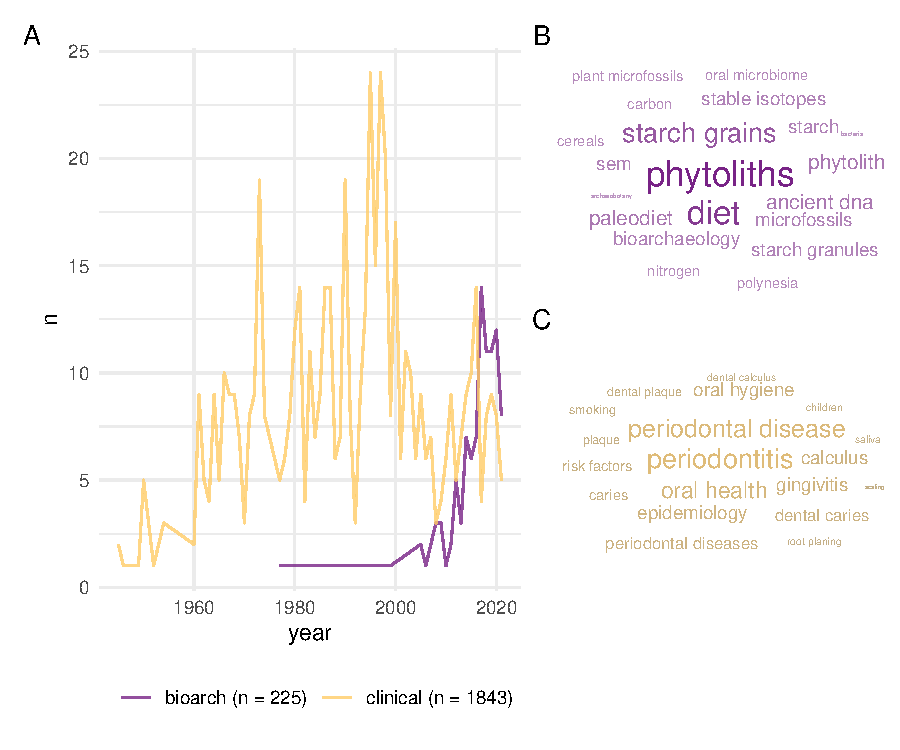
\includegraphics{01-intro_files/figure-pdf/fig-plot-and-wordclouds-1.pdf}

}

\caption{\label{fig-plot-and-wordclouds}Plot of the number of articles
per year in bioarchaeology and clinical dentistry with the term `dental
calculus' in the title.}

\end{figure}%

Perhaps the most common use of dental calculus is to recreate the diet
of past people and populations (Figure~\ref{fig-plot-and-wordclouds}B).
One of the ways to do this is by dissolving the calculus in a weak acid
or decalcifant, or mechanically breaking it up. This process releases
any fragments of plants that were trapped within the calculus and can be
identified, for example with a microscope. The tricky part is not
destroying the plant fragments when releasing them from the calculus. As
far as I can tell, the first attempt at this was the extraction of
phytoliths (silicified plant remains) from the teeth of cows, sheep, and
horses (\citeproc{ref-armitageExtractionIdentification1975}{Armitage,
1975}). This was a somewhat isolated use-case, and the method didn't
really catch on until the 1990s
(\citeproc{ref-ciochonOpalPhytoliths1990}{Ciochon et al., 1990};
Middleton 1990, in \citeproc{ref-middletonOpalPhytoliths1994}{Middleton
\& Rovner, 1994}). The first extractions from human teeth followed
shortly (\citeproc{ref-foxPhytolithCalculus1996}{Fox et al., 1996}), and
there are now studies using plant microremains (especially starch
granules and phytoliths) from dental calculus to infer diet in past
peoples from across the world, including Pacific Islands
(\citeproc{ref-dudgeonDietGeography2014}{Dudgeon \& Tromp, 2014}), China
(\citeproc{ref-chenStarchGrains2021}{Chen et al., 2021}), Europe
(\citeproc{ref-fiorinCombiningDental2021}{Fiorin et al., 2021}), and
more (\citeproc{ref-buckleyDentalCalculus2014}{Buckley et al., 2014};
\citeproc{ref-henryCalculusSyria2008}{Henry \& Piperno, 2008};
\citeproc{ref-mickleburghNewInsights2012}{Mickleburgh \& Pagán-Jiménez,
2012}). The durable nature of dental calculus also means that
microremains within it can survive for millennia, allowing us to look at
the diets of early humans and other hominins
(\citeproc{ref-buckleyDentalCalculus2014}{Buckley et al., 2014};
\citeproc{ref-chenStarchGrains2021}{Chen et al., 2021};
\citeproc{ref-hardyStarchGranules2009}{Hardy et al., 2009};
\citeproc{ref-hardyNeanderthalMedics2012}{Hardy et al., 2012};
\citeproc{ref-henryDietAustralopithecus2012}{Henry et al., 2012},
\citeproc{ref-henryNeanderthalCalculus2014}{2014};
\citeproc{ref-henryCalculusSyria2008}{Henry \& Piperno, 2008};
\citeproc{ref-pipernoStarchGrains2008}{Piperno \& Dillehay, 2008}).

That bacteria can become trapped within calculus has been known to
archaeologists for a while
(\citeproc{ref-brothwellDiggingBones1981}{Brothwell, 1981}, ;
\citeproc{ref-vandermeerschMiddlePaleolithic1994}{Vandermeersch et al.,
1994}), but it wasn't used in archaeological research until DNA
extraction started to become more accessible
(\citeproc{ref-delafuenteDNAHuman2013}{De La Fuente et al., 2013}).
Dental calculus then became part of the third scientific revolution in
archaeology. The early studies focused on oral health in the past
(\citeproc{ref-adlerSequencingAncient2013}{Adler et al., 2013};
\citeproc{ref-delafuenteDNAHuman2013}{De La Fuente et al., 2013};
\citeproc{ref-warinnerPathogensHost2014}{Warinner, Rodrigues, et al.,
2014}). Bacteria have shorter lifespans than humans which makes them
useful when studying the evolution of bacteria in the human mouth
(\citeproc{ref-delafuenteDNAHuman2013}{De La Fuente et al., 2013};
\citeproc{ref-yatesOralMicrobiome2021}{Fellows Yates et al., 2021}).
Diet has also been a focus of paleogenetic research. This has mainly
been addressed by considering how long-term changes in the patterns of
bacteria within the mouths of our ancestors have changed that could be
related to changes in diet. Just like we adapt to deal with various
diseases, climates, etc., we also adapt to changes in our diet
(\citeproc{ref-adlerSequencingAncient2013}{Adler et al., 2013};
\citeproc{ref-yatesOralMicrobiome2021}{Fellows Yates et al., 2021}).
Directly identifying genetic markers of plants and animals within dental
calculus is difficult, but not impossible (see Warinner, Hendy, et al.
(\citeproc{ref-warinnerEvidenceMilk2014}{2014})). Most of the DNA within
dental calculus will be oral bacteria, and this will overwhelm the small
signal from plant DNA, which makes species identifications problematic
(\citeproc{ref-fagernasMicrobialBiogeography2022}{Fagernäs et al.,
2022}). A newer field of biomolecular archaeology, paleoproteomics, may
be able to address this issue by targeting plant proteins, along with a
range of other dietary protein sources. Hendy and coauthors were able to
identify a number of these in dental calculus, as well as proteins from
cereals, and milk proteins from different sources
(\citeproc{ref-hendyProteomicCalculus2018}{Hendy et al., 2018}). Dental
calculus has also become a target for extracting other biomolecules that
may be related to diet, such as alkaloids, fatty acids, and
carbohydrates
(\citeproc{ref-gismondiMultidisciplinaryApproach2020}{Gismondi et al.,
2020}; \citeproc{ref-velskoDentalCalculus2017}{Velsko et al., 2017}).
The methods used for this have also proven to be useful in detecting
compounds that are related to other activities and ceremonies, such as
nicotine (\citeproc{ref-eerkensDentalCalculus2018}{Eerkens et al.,
2018}), and may provide some evidence of medicinal practices
(\citeproc{ref-gismondiMultidisciplinaryApproach2020}{Gismondi et al.,
2020}).

To a lesser extent, the presence and amount of dental calculus on teeth
has been used as an indicator of dental health
(\citeproc{ref-drewettExcavationOval1975}{Drewett, 1975};
\citeproc{ref-lieverseDentalHealth2007}{Lieverse et al., 2007};
\citeproc{ref-sagneStudiesPeriodontal1977}{Sagne \& Olsson, 1977};
\citeproc{ref-zhangDentalDisease1982}{Zhang, 1982}). Pilloud \& Fancher
(\citeproc{ref-pilloudOutliningDefinition2019}{2019}) explored the terms
associated with a number publications on dental or oral health, dental
calculus came up as one of them; albeit not the most common, which was
(unsurprisingly) dental caries (Figure~\ref{fig-dental-terms}).

To a lesser, lesser extent, it has also provided some interesting
insights on non-dietary activities, such as occupations and smoking
habits. In a rare find, blue particles were detected in the dental
calculus of a Medieval German woman. These blue particles originated
from lapis lazuli, an exotic stone often ground into pigments and used
to illuminate manuscripts (\citeproc{ref-radiniMedievalWomen2019}{Radini
et al., 2019}). Nicotine was detected in dental calculus of
pre-colonisation individuals from California using Ultra-Performance
Liquid Chromatography Mass Spectrometry (UPLC-MS), showing direct
consumption of tobacco and providing more detailed insights on the
demographics of consumption in a way that no other human-adjacent
archaeological materials can.

\begin{figure}

\centering{

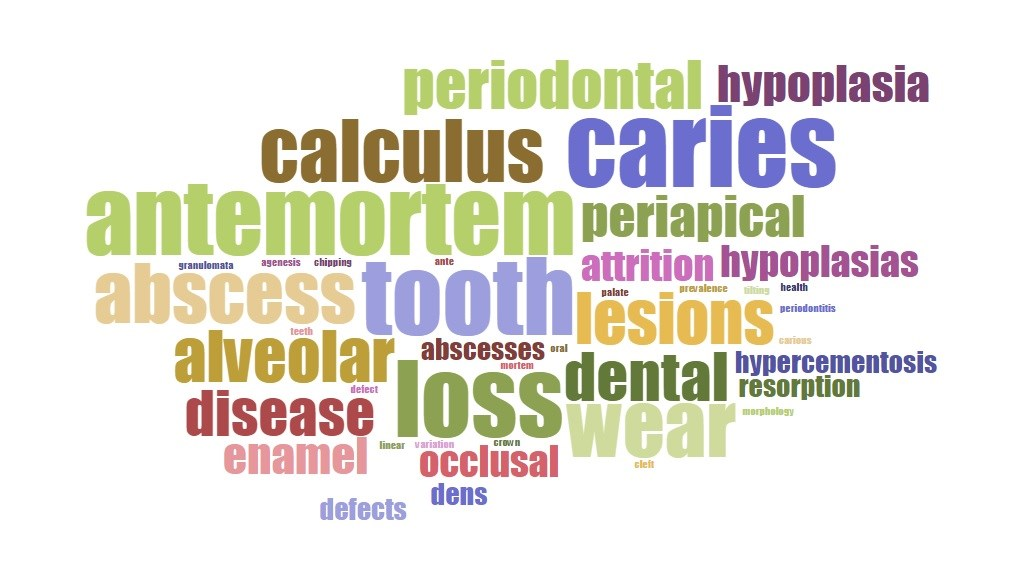
\includegraphics{figures/wordcloud.png}

}

\caption{\label{fig-dental-terms}Word cloud of most common dental terms
in articles. Figure is from Pilloud \& Fancher
(\citeproc{ref-pilloudOutliningDefinition2019}{2019}), Figure 1.}

\end{figure}%

It wasn't always appreciated for the wealth of information hidden within
its hardened shell. Until roughly 20 years ago, archaeologists who
encountered calculus had limited use for this material. Some researchers
quantified it using a simple four-stage scoring method that was
developed for recording deposits on archaeological dental calculus
(\citeproc{ref-brothwellDiggingBones1981}{Brothwell, 1981}), similar to
a common clinical scoring system
(\citeproc{ref-greeneSimplifiedOral1964}{J. G. Greene \& Vermillion,
1964}). The four-stage system is probably still the most widely used
among archaeologists. More detailed methods are also available
(\citeproc{ref-dobneyMethodEvaluating1987}{Dobney \& Brothwell, 1987};
\citeproc{ref-greeneQuantifyingCalculus2005}{T. R. Greene et al.,
2005}), but the original method is generally preferred for its
simplicity. Unfortunately, knowing the size of a calculus deposit is not
as valuable as being able to analyse the deposit itself, and the
deposits were often removed because they obscured tooth and root
morphology (\citeproc{ref-scottBriefHistory2015}{Scott, 2015}). This had
made a lot of people very angry and been widely regarded as a bad move
(\citeproc{ref-adamsRestaurantEnd2002}{Adams, 2002, p. 1}). Hindsight
being what it is, it's hard to blame anyone. A lot of dental research
mainly focuses on the prevention and removal of dental calculus.

The wide range of applications for dental calculus that we know about
today, and the fact that it's pretty much ubiquitous in the past thanks
to poor oral hygiene, makes it a really exciting target for future (and
current) paleodietary research. That being said, the study of dental
calculus doesn't seem to fit into any predefined areas of study within
(and beyond) archaeology. Most researchers seem to see it as a means to
the information contained within, rather than being worth studying in
its own right. This can be problematic. Other than what we can see with
our current methods, what do we really know about dental calculus and
how its growth and structure affect the reliability of these methods and
potentially distort our interpretations of the past?

\section{What is dental calculus?}\label{intro-what}

To answer these questions, we must first answer a single, surprisingly
difficult question: What is dental calculus? I'm not referring to its
formation or composition, which I briefly described
\hyperref[chap-intro]{above}. How do we categorise it? Is it a dental
disease? An oral health condition? A byproduct of oral conditions? We
start by exploring various definitions of oral health. Definitions in an
introduction are a little cliché and tedious, but often necessary. Since
oral health is a complex topic, definitions of oral health are often
purposefully (and confusingly) broad, and they extend beyond physical
well-being and into the realms of emotional and social comfort. The
World Dental Federation (FDI) defines oral health as the ability to
perform mouth- and face-related functions with confidence and without
pain (including smiling, speaking, eating, etc.)
(\citeproc{ref-fdiOralHealth}{{``{FDI}'s Definition of Oral Health
\textbar{} {FDI},''} n.d.})
(\url{https://www.fdiworlddental.org/fdis-definition-oral-health}). Both
the World Health Organisation (WHO) and FDI take a similar approach to
defining oral conditions, giving a list of conditions that cause
discomfort, pain, disfigurement, or death. The list includes the dental
conditions tooth decay (caries), gum disease (periodontal disease), and
dental trauma, but not dental calculus
(\citeproc{ref-whoOralHealth}{{``Oral Health,''} n.d.})
(\url{https://www.who.int/news-room/fact-sheets/detail/oral-health}).
While these are not likely to cause death, they are often the source of
physical and emotional discomfort, and may cause further health
complications if they are not dealt with in a timely fashion.

Dental calculus and dental plaque are not considered oral conditions
according to WHO. In fact, dental plaque is part of the normal
functioning of our oral biome
(\citeproc{ref-marshDentalPlaque2006}{Marsh, 2006}). When plaque reaches
a certain level of acidity over a prolonged period of time, the normal
functioning of the bacteria within the plaque may shift towards a
disease-causing function. The biofilm will cause the surface of the
enamel to demineralise, eventually resulting in a cavity (or caries).
Dental caries are unequivocally considered a dental disease. If,
instead, the biofilm calcifies, dental calculus is the result. Its
status in oral health is questionable.

Dental calculus is not known to be painful, nor does it affect the
ability to perform the functions listed above. However, with continued
accumulation, it may affect the confidence of the person performing
these tasks (\citeproc{ref-collinsHomelessDental2007}{Collins \&
Freeman, 2007}), and in extreme cases it can affect function
(\citeproc{ref-balajiUnusualPresentation2019}{Balaji et al., 2019}).
Most of the virulence and disease-causing potential is lost when the
bacteria within dental plaque calcify
(\citeproc{ref-akcaliDentalCalculus2018}{Akcalı \& Lang, 2018}). It has
been shown to contain pockets of living bacteria that can be detrimental
to oral and dental health
(\citeproc{ref-tanCalculusUltrastructure2004}{Tan, Gillam, et al.,
2004}; \citeproc{ref-tanBacterialViability2004}{Tan, Mordan, et al.,
2004}). The rough, porous surface of dental calculus is also a great
place for bacteria to attach more easily and develop a new layer of
plaque on the surface of the calculus. This is likely why there is often
a correlation (NOT causation) between dental calculus and periodontitis,
especially subgingival calculus
(\citeproc{ref-jepsenCalculusRemoval2011}{Jepsen et al., 2011};
\citeproc{ref-whiteDentalCalculus1997}{D. J. White, 1997}). Since it
seems to fulfill some of the criteria of an oral condition, it should be
considered as such, at least under the definitions provided by WHO and
FDI. Whether or not dental calculus can be considered an oral disease is
more questionable. While it does grow on the surface of teeth, it
doesn't seem to affect the underlying enamel. And while there is a
relationship with periodontal disease (which has been defined as a
dental disease), the nature of this relationship is still under debate,
with calculus likely being a secondary contributor
(\citeproc{ref-jepsenCalculusRemoval2011}{Jepsen et al., 2011}). As
such, we can probably limit the definition to an oral condition and not
necessarily a dental disease
(\citeproc{ref-pilloudOutliningDefinition2019}{Pilloud \& Fancher,
2019}). In fact, dental calculus is quite hard, so a layer of dental
calculus on a tooth can actually protect it from wearing down (although
there are better options).

\section{The study of dental calculus}\label{intro-study}

It seems that the researchers who are studying dental calculus approach
it from a wide range of different fields and backgrounds, including
genetics, proteomics, botany, and (bio)archaeology. The paleogeneticists
mine it for the wealth of information it contains on oral health and
disease in the past (\citeproc{ref-yatesOralMicrobiome2021}{Fellows
Yates et al., 2021}; \citeproc{ref-warinnerPathogensHost2014}{Warinner,
Rodrigues, et al., 2014}). Paleodiet researchers extract microremains
and residues from food (\citeproc{ref-henryCalculusSyria2008}{Henry \&
Piperno, 2008}; \citeproc{ref-mickleburghNewInsights2012}{Mickleburgh \&
Pagán-Jiménez, 2012}) to infer dietary practices. Bioarchaeologists use
its presence and amount to broadly infer diet, and dental and overall
health in a given population
(\citeproc{ref-belcastroContinuityDiscontinuity2007}{Belcastro et al.,
2007}; \citeproc{ref-lieverseDentalHealth2007}{Lieverse et al., 2007};
\citeproc{ref-novakDentalHealth2015}{Novak, 2015};
\citeproc{ref-slausDentalHealth2011}{Šlaus et al., 2011};
\citeproc{ref-yaussyCalculusSurvivorship2019}{Yaussy \& DeWitte, 2019}).
This leaves research output from studies of calculus scattered across
multiple venues, with no clear gathering point. I think it's fair to say
that dental calculus should be included in discussions of pathological
oral conditions, even if its role is secondary. But who is currently
studying dental calculus as a substance in its own right? And why do we
need to learn more about it if we're just interested in what's inside?
Related discussions have started to take place in recent years
(\citeproc{ref-bucchiComparisonsMethods2019}{Bucchi et al., 2019};
\citeproc{ref-radiniDirtyTeeth2022}{Radini \& Nikita, 2022};
\citeproc{ref-wrightAdvancingRefining2021}{Wright et al., 2021}).

The lack of a specific field of study for dental calculus to belong may
be related to how it's taught to students (and if it's taught at all).
Textbooks from the more established fields in bioarchaeology are
probably a good indicator of the teaching curricula, which also impacts
research focus. The most popular osteoarchaeology textbooks only briefly
mention dental calculus as more of a footnote than anything else. A
couple of lines describing what it is (usually `mineralised plaque') and
that it can contain food debris and bacteria T. D. White et al.
(\citeproc{ref-whiteHumanOsteology2011}{2011}). They're not wrong.
Diseases that manifest themselves in the skeleton as lesions on the
bones have a very clear home in paleopathology. No one questions whether
or not the degeneration of vertebrae from tuberculosis should be
included in the paleopathology textbooks (at least not as far as I'm
aware).

These textbooks often include chapters on dental disease, where more
detailed descriptions of dental calculus are usually found (e.g.
\citeproc{ref-robertsDentalDisease2007}{Roberts \& Manchester, 2007};
\citeproc{ref-waldronPalaeopathology2020}{Waldron, 2020}). Dental
caries, calculus' more famous sibling, will often get a few pages. In
some cases, dental calculus may even be hidden within a section on
periodontal disease or plaque
(\citeproc{ref-aufderheidePaleopathology1998}{Aufderheide et al., 1998};
e.g. \citeproc{ref-ortnerIdentificationPathological2003}{Ortner, 2003}).
The focus of these (sub)sections is varied, with some simply describing
what it is, and others giving brief discussion on the relationship
between calculus and periodontal disease. A more detailed section was
dedicated to dental calculus in \emph{Ortner's Identification of
Pathological Conditions in Human Skeletal Remains}, with a detailed
description of formation, structure, and application in (biomolecular)
archaeology (\citeproc{ref-kinastonOrtnerDentition2019}{Kinaston et al.,
2019}). The description extends well beyond any (paleo)pathological
significance of dental calculus. Can we fault the authors/editors for
not giving it more attention? After all, it's not a dental disease, and
its relationship with other dental diseases is unclear. What is clear,
is that it has implications for oral health, and, for that very reason,
could be addressed more extensively in paleopathology; certainly in the
textbooks that include dental disease.

On the surface, dental anthropology seems like a more suitable home for
the study of dental calculus. However, it's not included in \emph{A
Companion to Dental Anthropology}, an otherwise great resource on
studying archaeological teeth. The editors briefly acknowledge the
valuable information gained from calculus and that it holds a lot of
potential; but that's it (\citeproc{ref-scottBriefHistory2015}{Scott,
2015}). Other notable absences include textbooks such as \emph{Technique
and Application in Dental Anthropology} and \emph{New Direction in
Dental Anthropology}
(\citeproc{ref-townsendDentalAnthropology2012}{Townsend et al., 2012}),
both of which dedicate considerable attention to dental caries.
Hillson's \emph{Dental Anthropology}, a book that I consider to be the
`bible' for dental anthropology, has a section on dental calculus in the
Dental Disease chapter. It covers a basic description, the composition,
microscopic structure, methods used for recording archaeological
calculus, and the distribution in the dentition (i.e.~which teeth are
more prone to calculus buildup)
(\citeproc{ref-hillsonDentalAnthropology1996}{Hillson, 1996}).
Considering these are entire books devoted to the dentition, it seems
odd that there is often only a few paragraphs (if that) on dental
calculus. Granted, the only function teeth serve in the growth of dental
calculus is as a suitable surface on which to attach; though the role of
substratum is an important role, as dental calculus is seemingly unable
to form on other surfaces in the oral cavity.

Since the use of dental calculus in biomolecular archaeology is
relatively new, there are fewer available textbooks, and it rarely has a
dedicated course. The most common place to find descriptions of dental
calculus is, therefore, journal articles. There will be a short
paragraph on dental calculus formation (and sometimes composition) in
the introduction section. These are quite variable and are often limited
by the word count of the journal. Despite this, the descriptions will
often be as long, if not longer, than the sections in textbooks devoted
to dental calculus (\citeproc{ref-velskoMicrobialDifferences2019}{Velsko
et al., 2019}). The focus of these paragraphs are generally the same.
They describe the formation and mineral composition of dental calculus,
and provide some examples of how dental calculus has been used in
related studies (not unlike the beginning of this chapter). The
contribution of dental calculus to archaeology has been significant, so
it is likely to receive more and more attention going forward. In fact,
an entire chapter was recently devoted to dental calculus in the second
edition of \emph{Handbook of Archaeological Sciences}
(\citeproc{ref-fagernasDentalCalculus2023}{Fagernäs \& Warinner, 2023}).
Take that, dental caries!

\section{The challenges of studying dental
calculus}\label{the-challenges-of-studying-dental-calculus}

What we know about dental calculus and the influence of diet was
reviewed in an article aimed at (bio)archaeologists. The overall
conclusion reached in the article: it's still pretty unclear
(\citeproc{ref-lieverseDietAetiology1999}{Lieverse, 1999}). Now, 20-some
years later, there has been limited progress on this point. High-protein
diets are linked to an increase of urea, which is linked to an increase
in oral pH, which is linked to mineral deposition
(\citeproc{ref-dibdinOralUrea1998}{Dibdin \& Dawes, 1998};
\citeproc{ref-wongCalciumPhosphate2002}{Wong et al., 2002}). BUT,
protein may also inhibit crystalisation
(\citeproc{ref-hidakaDietCalculus2007}{S. Hidaka \& Oishi, 2007}).
Starch consumption has been linked to increased rates of caries in early
farming populations
(\citeproc{ref-storeyPaleopathologyOrigins1986}{Storey, 1986}). This is
consistent with \emph{in vitro} testing, at least for starches high in
amylose content. So a high-starch diet causes caries, not calculus,
right? Well, starches with a high amylopectin content are linked to
increased calcification (\citeproc{ref-hidakaDietCalculus2007}{S. Hidaka
\& Oishi, 2007}). It likely depends on what is consumed along with the
starch (\citeproc{ref-hidakaStarchRole2008}{Saburo Hidaka et al.,
2008}). There is also some (\emph{in vitro}) evidence to suggest that
silica may promote dental calculus formation by promoting mineral
precipitation, i.e.~the transfer of minerals from saliva to the biofilm
(\citeproc{ref-damenSilicicAcid1989}{Damen \& Ten Cate, 1989}). Overall,
this is an understudied area in both clinical and archaeological
contexts.

Another aspect of diet and dental calculus where we are still looking
for answers, is the process that causes fragments of food and other
environmental materials to become entrapped in the dental calculus. We
know that it happens. Decades of research has shown dental calculus to
be a seemingly unlimited resource for dietary substances. We don't know
exactly how this happens, and herein lies the potential for bias.
Efforts have been made to understand how much of the consumed food makes
it into the calculus. These include studies on modern humans
(\citeproc{ref-leonardPlantMicroremains2015}{Leonard et al., 2015}) and
non-human primates (\citeproc{ref-powerChimpCalculus2015}{R. C. Power et
al., 2015}; \citeproc{ref-powerRepresentativenessDental2021}{Robert C.
Power et al., 2021}), where food intake is meticulously documented, and
calculus subsequently analysed. These studies have common findings; the
amount of the diet that becomes trapped in the dental calculus of any
one person has no clear relationship to the amount of food that was
consumed. The most likely reason is that the formation of dental
calculus differs between people
(\citeproc{ref-powerChimpCalculus2015}{R. C. Power et al., 2015}). So,
it's not a great way to study the diet of a single person, but generally
suitable to study patterns in the diet of a population. The more people
you study, the more likely you are to gain a complete picture of the
diet in a population. The fact that we can still see (in some cases,
literally) remains that were consumed thousands of years ago is pretty
cool. We just need a better understanding of why the record of diet from
dental calculus differs from the actual intake of food. This will allow
us to make more robust interpretations about past dietary practices.
Something that may influence the dietary record that we get from
calculus is the method we use to extract the dietary remains from
calculus. Our understanding of dental calculus extraction methods is
improving, with studies looking at the effect of various acids used to
dissolve calculus (commonly EDTA or HCl)
(\citeproc{ref-bucchiComparisonsMethods2019}{Bucchi et al., 2019};
\citeproc{ref-palmerComparingUse2021}{Palmer et al., 2021};
\citeproc{ref-sotoCharacterizationDecontamination2019}{Soto et al.,
2019}; \citeproc{ref-trompEDTACalculus2017}{Tromp et al., 2017}); as is
our understanding of how the choice of tooth may affect our results
(\citeproc{ref-fagernasMicrobialBiogeography2021}{Fagernäs et al.,
2021}), and that not all we see is related to deliberate consumption
(\citeproc{ref-delaneyMoreWhat2023}{Delaney et al., 2023}).

These studies provide valuable insights into potential biases of our
sampling methods and the representation of diet within dental calculus,
with a minor caveat. Most of these studies have been conducted on living
primates or archaeological remains. An issue with using living (or once
living) organisms is the inability to control factors related to the
variability between subjects. Basically, studying humans is messy and
complicated because we're all unique. It's a lovely sentiment but it can
make for some messy science. Not bad science (not at all!). Just messy.
A method of study that offers more control is the growth of plaque and
calculus in a lab. This allows us to control many of the things that are
difficult to control in humans, such as the bacteria that colonise our
mouth, where each person has a pretty unique makeup of bacteria. We also
have a very unique genome (with the exception of identical twins) that
plays a role in how quickly we form calculus in our mouth (if at all).
Certain enzymes start digesting our food as soon as it enters our mouth,
and the activity of these enzymes fluctuates throughout the day, causing
a lot of variability both within and between individuals. Finally, the
number of microremains that enter our mouth over days, weeks, and
months, can be very different between people, even with the same diet.
All these things can muddy the results of research on living subjects,
where a lab-grown approach can help tease out confounding factors. I
don't believe research conducted on lab-grown biofilms can in any way
replace studies with modern or archaeological individuals, nor should
they. But it can complement these studies by zooming in on certain
aspects that are too difficult to isolate in (once-)living people.

Often we can draw from clinical studies as there are common goals,
e.g.~discovering the aetiology and/or presentation of a disease.
However, the motivation driving the studies in archaeology and dental
research are inherently different; although, there is certainly overlap
in some areas (Figure~\ref{fig-plot-and-wordclouds}B and C). There is
more interest in preventing dental calculus from forming in the first
place, so most studies focus on short-duration models to explore
anti-microbial treatments and inhibition of biofilm formation and plaque
buildup (\citeproc{ref-extercateAAA2010}{Exterkate et al., 2010}). As
shown in a previous study, calculus and plaque have distinct microbial
profiles (\citeproc{ref-velskoMicrobialDifferences2019}{Velsko et al.,
2019}), so the applicability of short-term models to explore
archaeological questions on dental calculus are limited, since plaque is
rarely (if ever) preserved. Archaeologists are more interested in
questions related to how diet influences the growth of biofilms, and how
fragments become embedded inside, and what we can say about diet.
Further, the interest in dental calculus as a field of clinical research
has been declining since the 2000s, which, as far as I'm aware, is when
the last studies growing dental calculus in a lab were conducted. We can
see this by the number of clinical articles with the term dental
calculus in the title (Figure~\ref{fig-plot-and-wordclouds}A). And they
certainly aren't interested in how food debris becomes trapped inside
our calculus. Dental calculus has also become less of a problem with the
use of modern dental hygiene practices and regular visits to the dentist
(\citeproc{ref-velskoMicrobialDifferences2019}{Velsko et al., 2019}).

To summarise: Bioarchaeologists are interested in how dental calculus
relates to dental and general health; paleodietary researchers are
interested in the food remains that are trapped inside; paleogeneticists
are interested in accessing the oral bacteria that have been fossilised
within; clinial dentistry views it as a nuisance to be removed and,
ideally, prevented from forming in the first place. This lack of
systematic research specifically devoted to dental calculus as a
substance, rather than a means to an end, leaves a lot of questions
regarding the expected behaviour of dental calculus and how information
from the past becomes trapped inside. To summarise the summary: we need
to ask more basic questions about dental calculus.

\section{Aims}\label{intro-aims}

This dissertation is a contribution to a dental-calculus-centric body of
knowledge, and addresses a gap in the fundamental research on dental
calculus to further our understanding of how we can use dental calculus
to reconstruct the diets of people in the past. The main aim is the
development, validation, and application of a calcifying oral biofilm
model to improve interpretations on archaeological dental calculus. By
developing a model system we can isolate the effects of confounding
factors in dental calculus and diet, and explore new uses for dental
calculus in paleodietary reconstructions through fundamental
experimentation. I also aim to assess the potential and limitations of
dental calculus to explore dietary activities of past populations.

Every decision we make, from sampling to statistical analysis, leads us
down a unique path towards a different interpretation from the other
possible paths in the multiverse of analyses. It's important we fully
understand the path we take, to ensure that it is the right path given
the limitations, and one that maximises the validity and detail of our
interpretations.

With these aims, I hope to address the following research questions:

\emph{How can we improve the resolution of our interpretations using
dental calculus on individuals and populations?} We are stuck in the
identification of compounds, and unable to speak to the quantity, since
we know that it's not very representative of a single individual.

\emph{Can we trust the system? (i.e., using dental calculus to
reconstruct diet)} Since we don't know the mechanism of incorporation,
there are likely hidden biases and limitations of our methods as a
result. We don't know the starting point, i.e., exactly what and how
much was originally trapped inside, so we have difficulty validating our
methods.

\emph{How can a model improve our understanding of dietary
reconstructions using dental calculus?} How can it address current
challenges in paleodietary reconstructions, and can it help us produce a
better understanding of how dietary intake relates to the record of diet
we extract from archaeological dental calculus?

\section{Thesis outline and
structure}\label{thesis-outline-and-structure}

If you have made it to this point, you have probably read most of
\hyperref[chap-intro]{\textbf{Chapter 1}}, in which I provide some
context to the study of dental calculus in archaeology and identify some
areas that could benefit from further investigation.
\hyperref[chap-background]{\textbf{Chapter 2}} provides some background
information on oral biofilms and oral biofilm models in more detail than
I can do in the research articles included in Chapters 3 and 4. So if
you're already well-versed in oral microbiology, feel free to skip to
Chapter 3. If not, I recommend picking up a textbook written by actual
experts in the field of oral microbiology. If, for some reason, you
can't access one of these, feel free to read
\hyperref[chap-background]{\textbf{Chapter 2}}. I suppose there are
worse options than something written by a PhD student in archaeology.
The chapter reflects the current knowledge of biofilms and the oral
microbiome (as best I could summarise) at the time of writing, and no
warranty is given for the inevitable new developments that will change
what we now believe to be true.

To address the aims of the dissertation outlined
\hyperref[intro-aims]{above}, I developed a protocol to grow dental
calculus in a lab on plastic tubes instead of looking at the real stuff
you normally find inside your mouth. The reason for using lab-grown
biofilms instead of humans is that the \emph{in vitro} lab model offers
more control over all the factors that go into the growth of dental
calculus, at least in theory. The real world is messy, and sometimes you
need to remove things from the real world to break it down and really
get into the nitty gritty of how it works. There are many different
kinds of biofilm models, including single species of bacteria, select
species determined by the researchers (defined consortium), and multiple
species from some natural source (the human mouth, for example). I will
cover the different types of models in more detail in
\hyperref[background]{\textbf{Chapter 2}}. Since there are many biofilm
models to choose from, developing a new protocol may seem
counter-productive; however, few are developed for long-term growth and
even fewer with the purpose of mineralising the biofilm to form dental
calculus. One of the exceptions involves a highly complex setup that is
unlikely to be supported by budgets and facilities available to most
archaeological laboratories
(\citeproc{ref-sissonsMultistationPlaque1991}{Sissons et al., 1991}).

After developing a working protocol, the next step was to determine if
the stuff I grew in the lab is actually dental calculus. Or at least
something close enough that we can use it to explore our research
questions. To do this, we (myself and coauthors) determined the mineral
and bacterial composition of our model using Fourier Transform Infrared
(FTIR) spectroscopy and metagenomic classification
\hyperref[byoc-valid]{\textbf{Chapter 3}}. We then compared the results
of these analyses to naturally grown dental calculus, both modern and
archaeological.

Being confident that our model looks and behaves like human dental
calculus, we then set out to test some very basic behaviours of starch
grains within dental calculus. \hyperref[byoc-starch]{\textbf{Chapter
4}} is a research article where we `fed' the biofilm with a known
quantity of starch granules during the growth period to see if the input
quantity/ratio matched the extracted quantity (or output). Those who are
familiar with dental calculus research will not be surprised that it did
not. The more interesting outcome of the study is the more detailed
explanation of how the input and output starch quantities were
mismatched.

\hyperref[mb11CalculusPilot]{\textbf{Chapter 5}} is a separate article,
in the sense that it doesn't involve the biofilm model in any way.
Rather, it addresses the theme of the overall utility of dental calculus
in archaeological research. We look at possible medicinal compounds in
the dental calculus of a Post-medieval Dutch population. We employed
Ultra High Performance Liquid Chromatography coupled with tandem Mass
Spectrometry (UHPLC-MS/MS) to identify various compounds in dental
calculus, including alkaloids and other compounds. It shows the
potential of dental calculus to inform about past practices, but also
highlights some of the limitations we are currently experiencing in the
field. \hyperref[chap-discussion]{\textbf{Chapter 6}} is a discussion on
the limitations and future potential of dental calculus in the field of
archaeology, and what biofilm models can contribute to our understanding
of past diet.

\section*{References cited}\label{references-cited}
\addcontentsline{toc}{section}{References cited}

\markright{References cited}

\phantomsection\label{refs-1}
\begin{CSLReferences}{1}{0}
\bibitem[\citeproctext]{ref-adamsRestaurantEnd2002}
Adams, D. (2002). \emph{The {Restaurant} at the {End} of the
{Universe}}. {Picador}.

\bibitem[\citeproctext]{ref-adlerSequencingAncient2013}
Adler, C. J., Dobney, K., Weyrich, L. S., Kaidonis, J., Walker, A. W.,
Haak, W., Bradshaw, C. J., Townsend, G., Sołtysiak, A., Alt, K. W.,
Parkhill, J., \& Cooper, A. (2013). Sequencing ancient calcified dental
plaque shows changes in oral microbiota with dietary shifts of the
{Neolithic} and {Industrial} revolutions. \emph{Nature Genetics},
\emph{45}(4), 450--455, 455e1. \url{https://doi.org/10.1038/ng.2536}

\bibitem[\citeproctext]{ref-akcaliDentalCalculus2018}
Akcalı, A., \& Lang, N. P. (2018). Dental calculus: The calcified
biofilm and its role in disease development. \emph{Periodontology 2000},
\emph{76}(1), 109--115. \url{https://doi.org/10.1111/prd.12151}

\bibitem[\citeproctext]{ref-armitageExtractionIdentification1975}
Armitage, P. L. (1975). The {Extraction} and {Identification} of {Opal
Phytoliths} from the {Teeth} of {Ungulates}. \emph{Journal of
Archaeological Science}, \emph{2}, 187--197.

\bibitem[\citeproctext]{ref-aufderheidePaleopathology1998}
Aufderheide, A. C., Rodriguez-Martin, C., \& Langsjoen, O. (1998).
\emph{The {Cambridge} encyclopedia of human paleopathology} (Vol. 478).
{Cambridge University Press Cambridge}.

\bibitem[\citeproctext]{ref-balajiUnusualPresentation2019}
Balaji, V. R., Niazi, T. M., \& Dhanasekaran, M. (2019). An unusual
presentation of dental calculus. \emph{Journal of Indian Society of
Periodontology}, \emph{23}(5), 484--486.
\url{https://doi.org/10.4103/jisp.jisp_680_18}

\bibitem[\citeproctext]{ref-belcastroContinuityDiscontinuity2007}
Belcastro, G., Rastelli, E., Mariotti, V., Consiglio, C., Facchini, F.,
\& Bonfiglioli, B. (2007). Continuity or discontinuity of the life-style
in central {Italy} during the {Roman} imperial age-early middle ages
transition: {Diet}, health, and behavior. \emph{American Journal of
Physical Anthropology}, \emph{132}(3), 381--394.
\url{https://doi.org/10.1002/ajpa.20530}

\bibitem[\citeproctext]{ref-brothwellDiggingBones1981}
Brothwell, D. (1981). \emph{Digging up {Bones}: {The} excavation,
treatment and study of human skeletal remains} (3rd ed.). {British
Museum (Natural History)}.

\bibitem[\citeproctext]{ref-bucchiComparisonsMethods2019}
Bucchi, A., Burguet-Coca, A., Expósito, I., Aceituno Bocanegra, F. J.,
\& Lozano, M. (2019). Comparisons between methods for analyzing dental
calculus samples from {El Mirador} cave ({Sierra} de {Atapuerca},
{Spain}). \emph{Archaeological and Anthropological Sciences},
\emph{11}(11), 6305--6314.
\url{https://doi.org/10.1007/s12520-019-00919-z}

\bibitem[\citeproctext]{ref-buckleyDentalCalculus2014}
Buckley, S., Usai, D., Jakob, T., Radini, A., \& Hardy, K. (2014).
Dental {Calculus Reveals Unique Insights} into {Food Items}, {Cooking}
and {Plant Processing} in {Prehistoric Central Sudan}. \emph{PLOS ONE},
\emph{9}(7), e100808. \url{https://doi.org/10.1371/journal.pone.0100808}

\bibitem[\citeproctext]{ref-charlierSEMCalculus2010}
Charlier, P., Huynh-Charlier, I., Munoz, O., Billard, M., Brun, L., \&
Grandmaison, G. L. de la. (2010). The microscopic (optical and {SEM})
examination of dental calculus deposits ({DCD}). {Potential} interest in
forensic anthropology of a bio-archaeological method. \emph{Legal
Medicine}, \emph{12}(4), 163--171.
\url{https://doi.org/10.1016/j.legalmed.2010.03.003}

\bibitem[\citeproctext]{ref-chenStarchGrains2021}
Chen, T., Hou, L., Jiang, H., Wu, Y., \& Henry, A. G. (2021). Starch
grains from human teeth reveal the plant consumption of proto-{Shang}
people (c. 2000\textendash 1600 {BC}) from {Nancheng} site, {Hebei},
{China}. \emph{Archaeological and Anthropological Sciences},
\emph{13}(9), 153. \url{https://doi.org/10.1007/s12520-021-01416-y}

\bibitem[\citeproctext]{ref-ciochonOpalPhytoliths1990}
Ciochon, R. L., Piperno, D. R., \& Thompson, R. G. (1990). Opal
phytoliths found on the teeth of the extinct ape {Gigantopithecus}
blacki: Implications for paleodietary studies. \emph{Proceedings of the
National Academy of Sciences}, \emph{87}(20), 8120--8124.
\url{https://doi.org/10.1073/pnas.87.20.8120}

\bibitem[\citeproctext]{ref-collinsHomelessDental2007}
Collins, J., \& Freeman, R. (2007). Homeless in {North} and {West
Belfast}: An oral health needs assessment. \emph{British Dental
Journal}, \emph{202}(12), E31--E31.
\url{https://doi.org/10.1038/bdj.2007.473}

\bibitem[\citeproctext]{ref-damenSilicicAcid1989}
Damen, J. J. M., \& Ten Cate, J. M. (1989). The {Effect} of {Silicic
Acid} on {Calcium Phosphate Precipitation}. \emph{Journal of Dental
Research}, \emph{68}(9), 1355--1359.
\url{https://doi.org/10.1177/00220345890680091301}

\bibitem[\citeproctext]{ref-delafuenteDNAHuman2013}
De La Fuente, C., Flores, S., \& Moraga, M. (2013). {DNA From Human
Ancient Bacteria}: {A} novel source of genetic evidence from
archaeological dental calculus. \emph{Archaeometry}, \emph{55}(4),
767--778. \url{https://doi.org/10.1111/j.1475-4754.2012.00707.x}

\bibitem[\citeproctext]{ref-delaneyMoreWhat2023}
Delaney, S., Alexander, M., \& Radini, A. (2023). More than what we eat:
{Investigating} an alternative pathway for intact starch granules in
dental calculus using {Experimental Archaeology}. \emph{Quaternary
International}, \emph{653--654}, 19--32.
\url{https://doi.org/10.1016/j.quaint.2022.03.004}

\bibitem[\citeproctext]{ref-dibdinOralUrea1998}
Dibdin, G. H., \& Dawes, C. (1998). A {Mathematical Model} of the
{Influence} of {Salivary Urea} on the {pH} of {Fasted Dental Plaque} and
on the {Changes Occurring} during a {Cariogenic Challenge}. \emph{Caries
Research}, \emph{32}(1), 70--74. \url{https://doi.org/10.1159/000016432}

\bibitem[\citeproctext]{ref-dobneyMethodEvaluating1987}
Dobney, K., \& Brothwell, D. (1987). A method for evaluating the amount
of dental calculus on teeth from archaeological sites. \emph{Journal of
Archaeological Science}, \emph{14}(4), 343--351.
\url{https://doi.org/10.1016/0305-4403(87)90024-0}

\bibitem[\citeproctext]{ref-drewettExcavationOval1975}
Drewett, P. (1975). \emph{The {Excavation} of an {Oval Burial Mound} of
the {Third Millennium} be at {Alfriston}, {East Sussex}, 1974}. 38.

\bibitem[\citeproctext]{ref-dudgeonDietGeography2014}
Dudgeon, J. V., \& Tromp, M. (2014). Diet, {Geography} and {Drinking
Water} in {Polynesia}: {Microfossil Research} from {Archaeological Human
Dental Calculus}, {Rapa Nui} ({Easter Island}). \emph{International
Journal of Osteoarchaeology}, \emph{24}(5), 634--648.
\url{https://doi.org/10.1002/oa.2249}

\bibitem[\citeproctext]{ref-eerkensDentalCalculus2018}
Eerkens, J. W., Tushingham, S., Brownstein, K. J., Garibay, R., Perez,
K., Murga, E., Kaijankoski, P., Rosenthal, J. S., \& Gang, D. R. (2018).
Dental calculus as a source of ancient alkaloids: {Detection} of
nicotine by {LC-MS} in calculus samples from the {Americas}.
\emph{Journal of Archaeological Science: Reports}, \emph{18}, 509--515.
\url{https://doi.org/10.1016/j.jasrep.2018.02.004}

\bibitem[\citeproctext]{ref-extercateAAA2010}
Exterkate, R. A. M., Crielaard, W., \& Ten Cate, J. M. (2010). Different
{Response} to {Amine Fluoride} by {Streptococcus} mutans and
{Polymicrobial Biofilms} in a {Novel High-Throughput Active Attachment
Model}. \emph{Caries Research}, \emph{44}(4), 372--379.
\url{https://doi.org/10.1159/000316541}

\bibitem[\citeproctext]{ref-fagernasMicrobialBiogeography2021}
Fagernäs, Z., Salazar-García, D. C., Avilés, A., Haber, M., Henry, A.,
Maurandi, J. L., Ozga, A., Velsko, I. M., \& Warinner, C. (2021).
Understanding the microbial biogeography of ancient human dentitions to
guide study design and interpretation. \emph{bioRxiv},
2021.08.16.456492. \url{https://doi.org/10.1101/2021.08.16.456492}

\bibitem[\citeproctext]{ref-fagernasMicrobialBiogeography2022}
Fagernäs, Z., Salazar-García, D. C., Haber Uriarte, M., Avilés
Fernández, A., Henry, A. G., Lomba Maurandi, J., Ozga, A. T., Velsko, I.
M., \& Warinner, C. (2022). Understanding the microbial biogeography of
ancient human dentitions to guide study design and interpretation.
\emph{FEMS Microbes}, \emph{3}, xtac006.
\url{https://doi.org/10.1093/femsmc/xtac006}

\bibitem[\citeproctext]{ref-fagernasDentalCalculus2023}
Fagernäs, Z., \& Warinner, C. (2023). Dental {Calculus}. In A. M.
Pollard, R. A. Armitage, \& C. Makarevicz (Eds.), \emph{Handbook of
{Archaeological Sciences}} (Second edition).

\bibitem[\citeproctext]{ref-fdiOralHealth}
{FDI}'s definition of oral health \textbar{} {FDI}. (n.d.). In \emph{FDI
World Dental Federation}.
https://www.fdiworlddental.org/fdis-definition-oral-health.

\bibitem[\citeproctext]{ref-yatesOralMicrobiome2021}
Fellows Yates, J. A., Velsko, I. M., Aron, F., Posth, C., Hofman, C. A.,
Austin, R. M., Parker, C. E., Mann, A. E., Nägele, K., Arthur, K. W.,
Arthur, J. W., Bauer, C. C., Crevecoeur, I., Cupillard, C., Curtis, M.
C., Dalén, L., Bonilla, M. D.-Z., Fernández-Lomana, J. C. D., Drucker,
D. G., \ldots{} Warinner, C. (2021). The evolution and changing ecology
of the {African} hominid oral microbiome. \emph{Proceedings of the
National Academy of Sciences}, \emph{118}(20).
\url{https://doi.org/10.1073/pnas.2021655118}

\bibitem[\citeproctext]{ref-fiorinCombiningDental2021}
Fiorin, E., Moore, J., Montgomery, J., Lippi, M. M., Nowell, G., \&
Forlin, P. (2021). Combining dental calculus with isotope analysis in
the {Alps}: {New} evidence from the {Roman} and medieval cemeteries of
{Lamon}, northern {Italy}. \emph{Quaternary International}.
\url{https://doi.org/10.1016/j.quaint.2021.11.022}

\bibitem[\citeproctext]{ref-foxPhytolithCalculus1996}
Fox, C. L., Juan, J., \& Albert, R. M. (1996). Phytolith analysis on
dental calculus, enamel surface, and burial soil: {Information} about
diet and paleoenvironment. \emph{American Journal of Physical
Anthropology}, \emph{101}(1), 101--113.
\url{https://doi.org/10.1002/(SICI)1096-8644(199609)101:1\%3C101::AID-AJPA7\%3E3.0.CO;2-Y}

\bibitem[\citeproctext]{ref-gismondiMultidisciplinaryApproach2020}
Gismondi, A., Baldoni, M., Gnes, M., Scorrano, G., D'Agostino, A.,
Marco, G. D., Calabria, G., Petrucci, M., Müldner, G., Tersch, M. V.,
Nardi, A., Enei, F., Canini, A., Rickards, O., Alexander, M., \&
Martínez-Labarga, C. (2020). A multidisciplinary approach for
investigating dietary and medicinal habits of the {Medieval} population
of {Santa Severa} (7th-15th centuries, {Rome}, {Italy}). \emph{PLOS
ONE}, \emph{15}(1), e0227433.
\url{https://doi.org/10.1371/journal.pone.0227433}

\bibitem[\citeproctext]{ref-greeneSimplifiedOral1964}
Greene, J. G., \& Vermillion, J. R. (1964). The {Simplified Oral Hygiene
Index}. \emph{The Journal of the American Dental Association},
\emph{68}(1), 7--13.
\url{https://doi.org/10.14219/jada.archive.1964.0034}

\bibitem[\citeproctext]{ref-greeneQuantifyingCalculus2005}
Greene, T. R., Kuba, C. L., \& Irish, J. D. (2005). Quantifying
calculus: {A} suggested new approach for recording an important
indicator of diet and dental health. \emph{HOMO - Journal of Comparative
Human Biology}, \emph{56}(2), 119--132.
\url{https://doi.org/10.1016/j.jchb.2005.02.002}

\bibitem[\citeproctext]{ref-hardyStarchGranules2009}
Hardy, K., Blakeney, T., Copeland, L., Kirkham, J., Wrangham, R., \&
Collins, M. (2009). Starch granules, dental calculus and new
perspectives on ancient diet. \emph{Journal of Archaeological Science},
\emph{36}(2), 248--255. \url{https://doi.org/10.1016/j.jas.2008.09.015}

\bibitem[\citeproctext]{ref-hardyNeanderthalMedics2012}
Hardy, K., Buckley, S., Collins, M. J., Estalrrich, A., Brothwell, D.,
Copeland, L., García-Tabernero, A., García-Vargas, S., de la Rasilla,
M., Lalueza-Fox, C., Huguet, R., Bastir, M., Santamaría, D., Madella,
M., Wilson, J., Cortés, Á. F., \& Rosas, A. (2012). Neanderthal medics?
{Evidence} for food, cooking, and medicinal plants entrapped in dental
calculus. \emph{Naturwissenschaften}, \emph{99}(8), 617--626.
\url{https://doi.org/10.1007/s00114-012-0942-0}

\bibitem[\citeproctext]{ref-hendyProteomicCalculus2018}
Hendy, J., Warinner, C., Bouwman, A., Collins, M. J., Fiddyment, S.,
Fischer, R., Hagan, R., Hofman, C. A., Holst, M., Chaves, E., Klaus, L.,
Larson, G., Mackie, M., McGrath, K., Mundorff, A. Z., Radini, A., Rao,
H., Trachsel, C., Velsko, I. M., \& Speller, C. F. (2018). Proteomic
evidence of dietary sources in ancient dental calculus.
\emph{Proceedings. Biological Sciences}, \emph{285}(1883), 20180977.
\url{https://doi.org/10.1098/rspb.2018.0977}

\bibitem[\citeproctext]{ref-henryNeanderthalCalculus2014}
Henry, A. G., Brooks, A. S., \& Piperno, D. R. (2014). Plant foods and
the dietary ecology of {Neanderthals} and early modern humans.
\emph{Journal of Human Evolution}, \emph{69}, 44--54.
\url{https://doi.org/10.1016/j.jhevol.2013.12.014}

\bibitem[\citeproctext]{ref-henryCalculusSyria2008}
Henry, A. G., \& Piperno, D. R. (2008). Using plant microfossils from
dental calculus to recover human diet: A case study from {Tell}
al-{Raqā}'i, {Syria}. \emph{Journal of Archaeological Science},
\emph{35}(7), 1943--1950.
\url{https://doi.org/10.1016/j.jas.2007.12.005}

\bibitem[\citeproctext]{ref-henryDietAustralopithecus2012}
Henry, A. G., Ungar, P. S., Passey, B. H., Sponheimer, M., Rossouw, L.,
Bamford, M., Sandberg, P., de Ruiter, D. J., \& Berger, L. (2012). The
diet of {Australopithecus} sediba. \emph{Nature}, \emph{487}(7405),
90--93. \url{https://doi.org/10.1038/nature11185}

\bibitem[\citeproctext]{ref-hidakaDietCalculus2007}
Hidaka, S., \& Oishi, A. (2007). An in vitro study of the effect of some
dietary components on calculus formation: Regulation of calcium
phosphate precipitation. \emph{Oral Diseases}, \emph{13}(3), 296--302.
\url{https://doi.org/10.1111/j.1601-0825.2006.01283.x}

\bibitem[\citeproctext]{ref-hidakaStarchRole2008}
Hidaka, Saburo, Okamoto, Y., Tsukamoto, S., \& Oishi, A. (2008). The
{Possible Role} of {Starch} in {Oral Calcification}: {The In Vitro
Formation} of {Hydroxyapatite} is {Regulated} by a {Combination} of
{Protein} and {Mineral Content} in {Dietary Starch Flour}. \emph{The
Open Food Science Journal}, \emph{2}(1), 10--22.
\url{https://doi.org/10.2174/1874256400802010010}

\bibitem[\citeproctext]{ref-hillsonDentalAnthropology1996}
Hillson, S. (1996). \emph{Dental {Anthropology}}. {Cambridge University
Press}.

\bibitem[\citeproctext]{ref-jepsenCalculusRemoval2011}
Jepsen, S., Deschner, J., Braun, A., Schwarz, F., \& Eberhard, J.
(2011). Calculus removal and the prevention of its formation.
\emph{Periodontology 2000}, \emph{55}(1), 167--188.
\url{https://doi.org/10.1111/j.1600-0757.2010.00382.x}

\bibitem[\citeproctext]{ref-jinSupragingivalCalculus2002}
Jin, Y., \& Yip, H.-K. (2002). Supragingival {Calculus}: {Formation} and
{Control}. \emph{Critical Reviews in Oral Biology \& Medicine}.
\url{https://doi.org/10.1177/154411130201300506}

\bibitem[\citeproctext]{ref-kinastonOrtnerDentition2019}
Kinaston, R., Willis, A., Miszkiewicz, J. J., Tromp, M., \& Oxenham, M.
F. (2019). The {Dentition}: {Development}, {Disturbances}, {Disease},
{Diet}, and {Chemistry}. In J. E. Buikstra (Ed.), \emph{Ortner's
{Identification} of {Pathological Conditions} in {Human Skeletal
Remains} ({Third Edition})} (pp. 749--797). {Academic Press}.
\url{https://doi.org/10.1016/B978-0-12-809738-0.00021-1}

\bibitem[\citeproctext]{ref-leonardPlantMicroremains2015}
Leonard, C., Vashro, L., O'Connell, J. F., \& Henry, A. G. (2015). Plant
microremains in dental calculus as a record of plant consumption: {A}
test with {Twe} forager-horticulturalists. \emph{Journal of
Archaeological Science: Reports}, \emph{2}, 449--457.
\url{https://doi.org/10.1016/j.jasrep.2015.03.009}

\bibitem[\citeproctext]{ref-lieverseDietAetiology1999}
Lieverse, A. R. (1999). Diet and the aetiology of dental calculus.
\emph{International Journal of Osteoarchaeology}, \emph{9}(4), 219--232.
\url{https://doi.org/10.1002/(SICI)1099-1212(199907/08)9:4\%3C219::AID-OA475\%3E3.0.CO;2-V}

\bibitem[\citeproctext]{ref-lieverseDentalHealth2007}
Lieverse, A. R., Link, D. W., Bazaliiskiy, V. I., Goriunova, O. I., \&
Weber, A. W. (2007). Dental health indicators of
hunter\textendash gatherer adaptation and cultural change in {Siberia}'s
{Cis-Baikal}. \emph{American Journal of Physical Anthropology},
\emph{134}(3), 323--339. \url{https://doi.org/10.1002/ajpa.20672}

\bibitem[\citeproctext]{ref-marshDentalPlaque2006}
Marsh, P. D. (2006). Dental plaque as a biofilm and a microbial
community \textendash{} implications for health and disease. \emph{BMC
Oral Health}, \emph{6}(S1), S14.
\url{https://doi.org/10.1186/1472-6831-6-S1-S14}

\bibitem[\citeproctext]{ref-mickleburghNewInsights2012}
Mickleburgh, H. L., \& Pagán-Jiménez, J. R. (2012). New insights into
the consumption of maize and other food plants in the pre-{Columbian
Caribbean} from starch grains trapped in human dental calculus.
\emph{Journal of Archaeological Science}, \emph{39}(7), 2468--2478.
\url{https://doi.org/10.1016/j.jas.2012.02.020}

\bibitem[\citeproctext]{ref-middletonOpalPhytoliths1994}
Middleton, W. D., \& Rovner, I. (1994). Extraction of {Opal Phytoliths}
from {Herbivore Dental Calculus}. \emph{Journal of Archaeological
Science}, \emph{21}(4), 469--473.
\url{https://doi.org/10.1006/jasc.1994.1046}

\bibitem[\citeproctext]{ref-novakDentalHealth2015}
Novak, M. (2015). Dental health and diet in early medieval {Ireland}.
\emph{Archives of Oral Biology}, \emph{60}(9), 1299--1309.
\url{https://doi.org/10.1016/j.archoralbio.2015.06.004}

\bibitem[\citeproctext]{ref-whoOralHealth}
Oral health. (n.d.). In \emph{World Health Organization}.
https://www.who.int/news-room/fact-sheets/detail/oral-health.

\bibitem[\citeproctext]{ref-ortnerIdentificationPathological2003}
Ortner, D. J. (2003). \emph{Identification of {Pathological Conditions}
in {Human Skeletal Remains}}. {Academic Press}.

\bibitem[\citeproctext]{ref-palmerComparingUse2021}
Palmer, K. S., Makarewicz, C. A., Tishkin, A. A., Tur, S. S., Chunag,
A., Diimajav, E., Jamsranjav, B., \& Buckley, M. (2021). Comparing the
{Use} of {Magnetic Beads} with {Ultrafiltration} for {Ancient Dental
Calculus Proteomics}. \emph{Journal of Proteome Research}, \emph{20}(3),
1689--1704. \url{https://doi.org/10.1021/acs.jproteome.0c00862}

\bibitem[\citeproctext]{ref-pilloudOutliningDefinition2019}
Pilloud, M. A., \& Fancher, J. P. (2019). Outlining a {Definition} of
{Oral Health} within the {Study} of {Human Skeletal Remains}: {Defining
Oral Health}. \emph{Dental Anthropology Journal}, \emph{32}(2), 3--11.
\url{https://doi.org/10.26575/daj.v32i2.297}

\bibitem[\citeproctext]{ref-pipernoStarchGrains2008}
Piperno, D. R., \& Dillehay, T. D. (2008). Starch grains on human teeth
reveal early broad crop diet in northern {Peru}. \emph{Proceedings of
the National Academy of Sciences}, \emph{105}(50), 19622--19627.
\url{https://doi.org/10.1073/pnas.0808752105}

\bibitem[\citeproctext]{ref-powerSynchrotronRadiationbased2022}
Power, Robert C., Henry, A. G., Moosmann, J., Beckmann, F., Temming, H.,
Roberts, A., \& Cabec, A. L. (2022). Synchrotron radiation-based
phase-contrast microtomography of human dental calculus allows
nondestructive analysis of inclusions: Implications for archeological
samples. \emph{Journal of Medical Imaging}, \emph{9}(3), 031505.
\url{https://doi.org/10.1117/1.JMI.9.3.031505}

\bibitem[\citeproctext]{ref-powerChimpCalculus2015}
Power, R. C., Salazar-Garcia, D. C., Wittig, R. M., Freiberg, M., \&
Henry, A. G. (2015). Dental calculus evidence of {Tai Forest Chimpanzee}
plant consumption and life history transitions. \emph{Scientific
Reports}, \emph{5}, 15161. \url{https://doi.org/10.1038/srep15161}

\bibitem[\citeproctext]{ref-powerRepresentativenessDental2021}
Power, Robert C., Wittig, R. M., Stone, J. R., Kupczik, K., \&
Schulz-Kornas, E. (2021). The representativeness of the dental calculus
dietary record: Insights from {Taï} chimpanzee faecal phytoliths.
\emph{Archaeological and Anthropological Sciences}, \emph{13}(6), 104.
\url{https://doi.org/10.1007/s12520-021-01342-z}

\bibitem[\citeproctext]{ref-radiniDirtyTeeth2022}
Radini, A., \& Nikita, E. (2022). Beyond dirty teeth: {Integrating}
dental calculus studies with osteoarchaeological parameters.
\emph{Quaternary International}.
\url{https://doi.org/10.1016/j.quaint.2022.03.003}

\bibitem[\citeproctext]{ref-radiniMedievalWomen2019}
Radini, A., Tromp, M., Beach, A., Tong, E., Speller, C., McCormick, M.,
Dudgeon, J. V., Collins, M. J., Rühli, F., Kröger, R., \& Warinner, C.
(2019). Medieval women's early involvement in manuscript production
suggested by lapis lazuli identification in dental calculus.
\emph{Science Advances}, \emph{5}(1), eaau7126.
\url{https://doi.org/10.1126/sciadv.aau7126}

\bibitem[\citeproctext]{ref-robertsDentalDisease2007}
Roberts, C. A., \& Manchester, K. (2007). Dental {Disease}. In \emph{The
{Archaeology} of {Disease}} (3rd Edition, pp. 63--83). {Cornell
University Press}.

\bibitem[\citeproctext]{ref-sagneStudiesPeriodontal1977}
Sagne, S., \& Olsson, G. (1977). Studies of the {Periodontal Status} of
a {Medieval Population}. \emph{Dentomaxillofacial Radiology},
\emph{6}(1), 46--52. \url{https://doi.org/10.1259/dmfr.1977.0006}

\bibitem[\citeproctext]{ref-scottBriefHistory2015}
Scott, G. R. (2015). A {Brief History} of {Dental Anthropology}. In J.
D. Irish \& G. R. Scott (Eds.), \emph{A {Companion} to {Dental
Anthropology}} (pp. 7--17). {John Wiley \& Sons, Ltd}.
\url{https://doi.org/10.1002/9781118845486.ch18}

\bibitem[\citeproctext]{ref-sissonsMultistationPlaque1991}
Sissons, C. H., Cutress, T. W., Hoffman, M. P., \& Wakefield, J. S. J.
(1991). A {Multi-station Dental Plaque Microcosm} ({Artificial Mouth})
for the {Study} of {Plaque Growth}, {Metabolism}, {pH}, and
{Mineralization}: \emph{Journal of Dental Research}.
\url{https://doi.org/10.1177/00220345910700110301}

\bibitem[\citeproctext]{ref-slausDentalHealth2011}
Šlaus, M., Bedić, Ž., Rajić Šikanjić, P., Vodanović, M., \& Domić Kunić,
A. (2011). Dental health at the transition from the {Late Antique} to
the early {Medieval} period on {Croatia}'s eastern {Adriatic} coast.
\emph{International Journal of Osteoarchaeology}, \emph{21}(5),
577--590. \url{https://doi.org/10.1002/oa.1163}

\bibitem[\citeproctext]{ref-sotoCharacterizationDecontamination2019}
Soto, M., Inwood, J., Clarke, S., Crowther, A., Covelli, D., Favreau,
J., Itambu, M., Larter, S., Lee, P., Lozano, M., Maley, J., Mwambwiga,
A., Patalano, R., Sammynaiken, R., Vergès, J. M., Zhu, J., \& Mercader,
J. (2019). Structural characterization and decontamination of dental
calculus for ancient starch research. \emph{Archaeological and
Anthropological Sciences}, \emph{11}(9), 4847--4872.
\url{https://doi.org/10.1007/s12520-019-00830-7}

\bibitem[\citeproctext]{ref-squierOralMucosa1998}
Squier, C. A., \& Finkelstein, M. W. (1998). Oral {Mucosa}. In A. R. Ten
Cate (Ed.), \emph{Oral {Histology}: {Development}, {Structure}, and
{Function}} (Fifth, pp. 345--385). {Mosby}.

\bibitem[\citeproctext]{ref-storeyPaleopathologyOrigins1986}
Storey, R. (1986). Paleopathology at the {Origins} of {Agriculture}.
{Mark Nathan Cohen} and {George J}. {Armelagos}, editors. {Academic
Press}, {Inc}., {Orlando}, 1984. Xx + 615 pp., figures, tables,
references, index. \$59.00 (cloth). \emph{American Antiquity},
\emph{51}(3), 661--662. \url{https://doi.org/10.2307/281762}

\bibitem[\citeproctext]{ref-tanCalculusUltrastructure2004}
Tan, B. T. K., Gillam, D. G., Mordan, N. J., \& Galgut, P. N. (2004). A
preliminary investigation into the ultrastructure of dental calculus and
associated bacteria. \emph{Journal of Clinical Periodontology},
\emph{31}(5), 364--369.
\url{https://doi.org/10.1111/j.1600-051X.2004.00484.x}

\bibitem[\citeproctext]{ref-tanBacterialViability2004}
Tan, B. T. K., Mordan, N. J., Embleton, J., Pratten, J., \& Galgut, P.
N. (2004). Study of {Bacterial Viability} within {Human Supragingival
Dental Calculus}. \emph{Journal of Periodontology}, \emph{75}(1),
23--29. \url{https://doi.org/10.1902/jop.2004.75.1.23}

\bibitem[\citeproctext]{ref-townsendDentalAnthropology2012}
Townsend, G., Kanazawa, E., \& Takayama, H. (Eds.). (2012). \emph{New
{Directions} in {Dental Anthropology}: {Paradigms}, {Methodologies} and
{Outcomes}}. {The University of Adelaide Press}.
\url{https://doi.org/10.1017/9780987171870}

\bibitem[\citeproctext]{ref-trompEDTACalculus2017}
Tromp, M., Buckley, H., Geber, J., \& Matisoo-Smith, E. (2017). {EDTA}
decalcification of dental calculus as an alternate means of
microparticle extraction from archaeological samples. \emph{Journal of
Archaeological Science: Reports}, \emph{14}, 461--466.
\url{https://doi.org/10.1016/j.jasrep.2017.06.035}

\bibitem[\citeproctext]{ref-vandermeerschMiddlePaleolithic1994}
Vandermeersch, B., Arensburg, B., Tillier, A. M., Rak, Y., Weiner, S.,
Spiers, M., \& Aspillaga, E. (1994). Middle {Paleolithic Dental Bacteria
From Kebara}, {Israel}. \emph{Comptes Rendus De L Academie Des Sciences
Serie Ii}, \emph{319}(6), 727--731.

\bibitem[\citeproctext]{ref-velskoMicrobialDifferences2019}
Velsko, I. M., Fellows Yates, J. A., Aron, F., Hagan, R. W., Frantz, L.
A. F., Loe, L., Martinez, J. B. R., Chaves, E., Gosden, C., Larson, G.,
\& Warinner, C. (2019). Microbial differences between dental plaque and
historic dental calculus are related to oral biofilm maturation stage.
\emph{Microbiome}, \emph{7}(1), 102.
\url{https://doi.org/10.1186/s40168-019-0717-3}

\bibitem[\citeproctext]{ref-velskoDentalCalculus2017}
Velsko, I. M., Overmyer, K. A., Speller, C., Klaus, L., Collins, M. J.,
Loe, L., Frantz, L. A. F., Sankaranarayanan, K., Lewis, C. M., Martinez,
J. B. R., Chaves, E., Coon, J. J., Larson, G., \& Warinner, C. (2017).
The dental calculus metabolome in modern and historic samples.
\emph{Metabolomics}, \emph{13}(11), 134.
\url{https://doi.org/10.1007/s11306-017-1270-3}

\bibitem[\citeproctext]{ref-waldronPalaeopathology2020}
Waldron, T. (2020). \emph{Palaeopathology}. {Cambridge University
Press}.

\bibitem[\citeproctext]{ref-warinnerEvidenceMilk2014}
Warinner, C., Hendy, J., Speller, C., Cappellini, E., Fischer, R.,
Trachsel, C., Arneborg, J., Lynnerup, N., Craig, O. E., Swallow, D. M.,
Fotakis, A., Christensen, R. J., Olsen, J. V., Liebert, A., Montalva,
N., Fiddyment, S., Charlton, S., Mackie, M., Canci, A., \ldots{}
Collins, M. J. (2014). Direct evidence of milk consumption from ancient
human dental calculus. \emph{Scientific Reports}, \emph{4}, 7104.
\url{https://doi.org/10.1038/srep07104}

\bibitem[\citeproctext]{ref-warinnerPathogensHost2014}
Warinner, C., Rodrigues, J. F., Vyas, R., Trachsel, C., Shved, N.,
Grossmann, J., Radini, A., Hancock, Y., Tito, R. Y., Fiddyment, S.,
Speller, C., Hendy, J., Charlton, S., Luder, H. U., Salazar-Garcia, D.
C., Eppler, E., Seiler, R., Hansen, L. H., Castruita, J. A., \ldots{}
Cappellini, E. (2014). Pathogens and host immunity in the ancient human
oral cavity. \emph{Nature Genetics}, \emph{46}(4), 336--344.
\url{https://doi.org/10.1038/ng.2906}

\bibitem[\citeproctext]{ref-warinnerNewEra2015}
Warinner, C., Speller, C., \& Collins, M. J. (2015). A new era in
palaeomicrobiology: Prospects for ancient dental calculus as a long-term
record of the human oral microbiome. \emph{Philosophical Transactions of
the Royal Society B: Biological Sciences}, \emph{370}(1660), 20130376.
\url{https://doi.org/10.1098/rstb.2013.0376}

\bibitem[\citeproctext]{ref-whiteDentalCalculus1997}
White, D. J. (1997). Dental calculus: Recent insights into occurrence,
formation, prevention, removal and oral health effects of supragingival
and subgingival deposits. \emph{European Journal of Oral Sciences},
\emph{105}(5), 508--522.
\url{https://doi.org/10.1111/j.1600-0722.1997.tb00238.x}

\bibitem[\citeproctext]{ref-whiteHumanOsteology2011}
White, T. D., Black, M. T., \& Folkens, P. A. (2011). \emph{Human
{Osteology}} (3rd edition). {Academic Press}.

\bibitem[\citeproctext]{ref-whiteBoneManual2005}
White, T. D., \& Folkens, P. A. (2005). \emph{The {Human Bone Manual}}
(1st edition). {Academic Press}.

\bibitem[\citeproctext]{ref-wongCalciumPhosphate2002}
Wong, L., Sissons, C. H., Pearce, E. I. F., \& Cutress, T. W. (2002).
Calcium phosphate deposition in human dental plaque microcosm biofilms
induced by a ureolytic {pH-rise} procedure. \emph{Archives of Oral
Biology}, \emph{47}(11), 779--790.
\url{https://doi.org/10.1016/S0003-9969(02)00114-0}

\bibitem[\citeproctext]{ref-wrightAdvancingRefining2021}
Wright, S. L., Dobney, K., \& Weyrich, L. S. (2021). Advancing and
refining archaeological dental calculus research using multiomic
frameworks. \emph{STAR: Science \& Technology of Archaeological
Research}, \emph{7}(1), 13--30.
\url{https://doi.org/10.1080/20548923.2021.1882122}

\bibitem[\citeproctext]{ref-yaussyCalculusSurvivorship2019}
Yaussy, S. L., \& DeWitte, S. N. (2019). Calculus and survivorship in
medieval {London}: {The} association between dental disease and a
demographic measure of general health. \emph{American Journal of
Physical Anthropology}, \emph{168}(3), 552--565.
\url{https://doi.org/10.1002/ajpa.23772}

\bibitem[\citeproctext]{ref-zhangDentalDisease1982}
Zhang, Y. (1982). Dental disease of neolithic age skulls excavated in
shaanxi province. \emph{Chinese Medical Journal}, \emph{95}(06),
391--396. \url{https://doi.org/10.5555/cmj.0366-6999.95.06.p391.01}

\end{CSLReferences}

\bookmarksetup{startatroot}

\chapter{Background}\label{chap-background}

The human mouth, or oral cavity, contains many different types of
surfaces on which bacteria can attach and grow. These surfaces are both
hard (teeth) and soft (mucosa, tongue, gingiva), and are exposed to the
external environment. For this reason, the conditions within the oral
cavity can vary considerably, resulting in a unique range of habitats
for a wide variety of microbes. In fact, the oral biome contains
bacteria from over 700 different species, some of which still haven't
been named, or even cultured. There are so many bacteria in our mouth
that it's actually hard to determine how many there are at any given
time, but most estimates are in the billions. Some like stable
temperatures and lots of oxygen. Others are better at dealing with
fluctuations in temperature and oxygen availability. Some can fend for
themselves and take what they need from the environment. Others depend
on the presence of other species to break down their food into smaller
pieces. Some like acidity. Others like alkalinity. So how can they all
seemingly thrive in the same place at the same time? The answer is
biofilms.

As an archaeologist, you may be wondering why you need to know all this
stuff. Dental calculus is the result of a very complex series of events
that involves the physiology of saliva, particular diets, age, genetics,
and a bunch of other things. To better understand what we see when we
analyse archaeological dental calculus to get at diet, we need to
understand all of the processes that went into forming it in the first
place. Only then can we begin to fully unlock its potential in
reconstructing past diets. In any case, we all have mouths, so on some
level I'm sure this knowledge will be relevant.

\section{Oral biofilms}\label{background-biofilms}

The concept of biofilms represents a recent paradigm shift in
microbiology (\citeproc{ref-costertonBacterialBiofilms1987}{Costerton et
al., 1987}, \citeproc{ref-costertonMicrobialBiofilms1995}{1995}).
Previously, researchers believed that you could isolate the organism of
interest and learn about its growth, metabolism, etc. They assumed
bacteria would behave the same as a free-floating organism in a lab test
tube as it would in a real-world environment (such as the human mouth).
More recently researchers have discovered that the behaviour of bacteria
differs when they are part of a larger community, compared to when they
are grown in isolation. Biofilms consist of large, intricate,
multi-species communities of bacteria enclosed in an extracellular
matrix of their own creation. The ability to produce this matrix gives
the bacteria living within it an adaptive advantage compared to
free-floating (planktonic) organisms. It equips them with resistance to
both antimicrobials (such as antibiotic medication) and immune responses
from the host that would normally be detrimental to their ability to
survive (\citeproc{ref-marshDentalPlaque2005}{Marsh, 2005};
\citeproc{ref-marshPhysiologicalApproaches1997}{Marsh \& Bradshaw,
1997}). Resistance to varying conditions is especially important in the
oral cavity, which is a site of frequent fluctuations in temperature,
pH, and oxygen availability. The viscoelastic nature of the biofilm
provides some protection against mechanical destruction and dislodgement
caused by, for example, the tongue and dental hygiene practices
(\citeproc{ref-petersonViscoelasticityBiofilms2015}{Peterson et al.,
2015}). It also allows them to acquire nutrients from outside the
biofilm, as well as generate and distribute nutrients within the biofilm
to the various communities of bacteria residing inside
(\citeproc{ref-flemmingBiofilmsEmergent2016}{Flemming et al., 2016}).
Biofilms are quite persistent structures, and very few surfaces exist
that can completely prevent bacterial colonisation and biofilm formation
(\citeproc{ref-rennerPhysicochemicalRegulation2011}{Renner \& Weibel,
2011}).

\subsection{Dental plaque}\label{dental-plaque}

Dental calculus forms from a specific oral biofilm known as dental
plaque. After we clean our teeth, our saliva coats the surface of our
teeth (enamel) with a layer of proteins known as the dental pellicle (or
acquired enamel pellicle). The pellicle is a film that protects our
teeth from both mechanical wear and chemical decay, but in doing so,
provides a viable surface for microorganisms to attach and initiate
biofilm growth (\citeproc{ref-yaoIdentificationProtein2003}{Yao et al.,
2003}). Biofilm formation goes through several, often arbitrarily
defined, stages of growth. They are arbitrary because they are defined
by the researchers who study them, but are also necessary as a
foundation to explain the development of a biofilm. Rather than thinking
about the stages as occurring sequentially, you should think of them as
occurring concurrently across different areas of the tooth surface.
Biofilm formation is a very dynamic process, and is often
over-simplified in visualisations (not unlike
Figure~\ref{fig-biofilm-form}).

\begin{figure}

\centering{

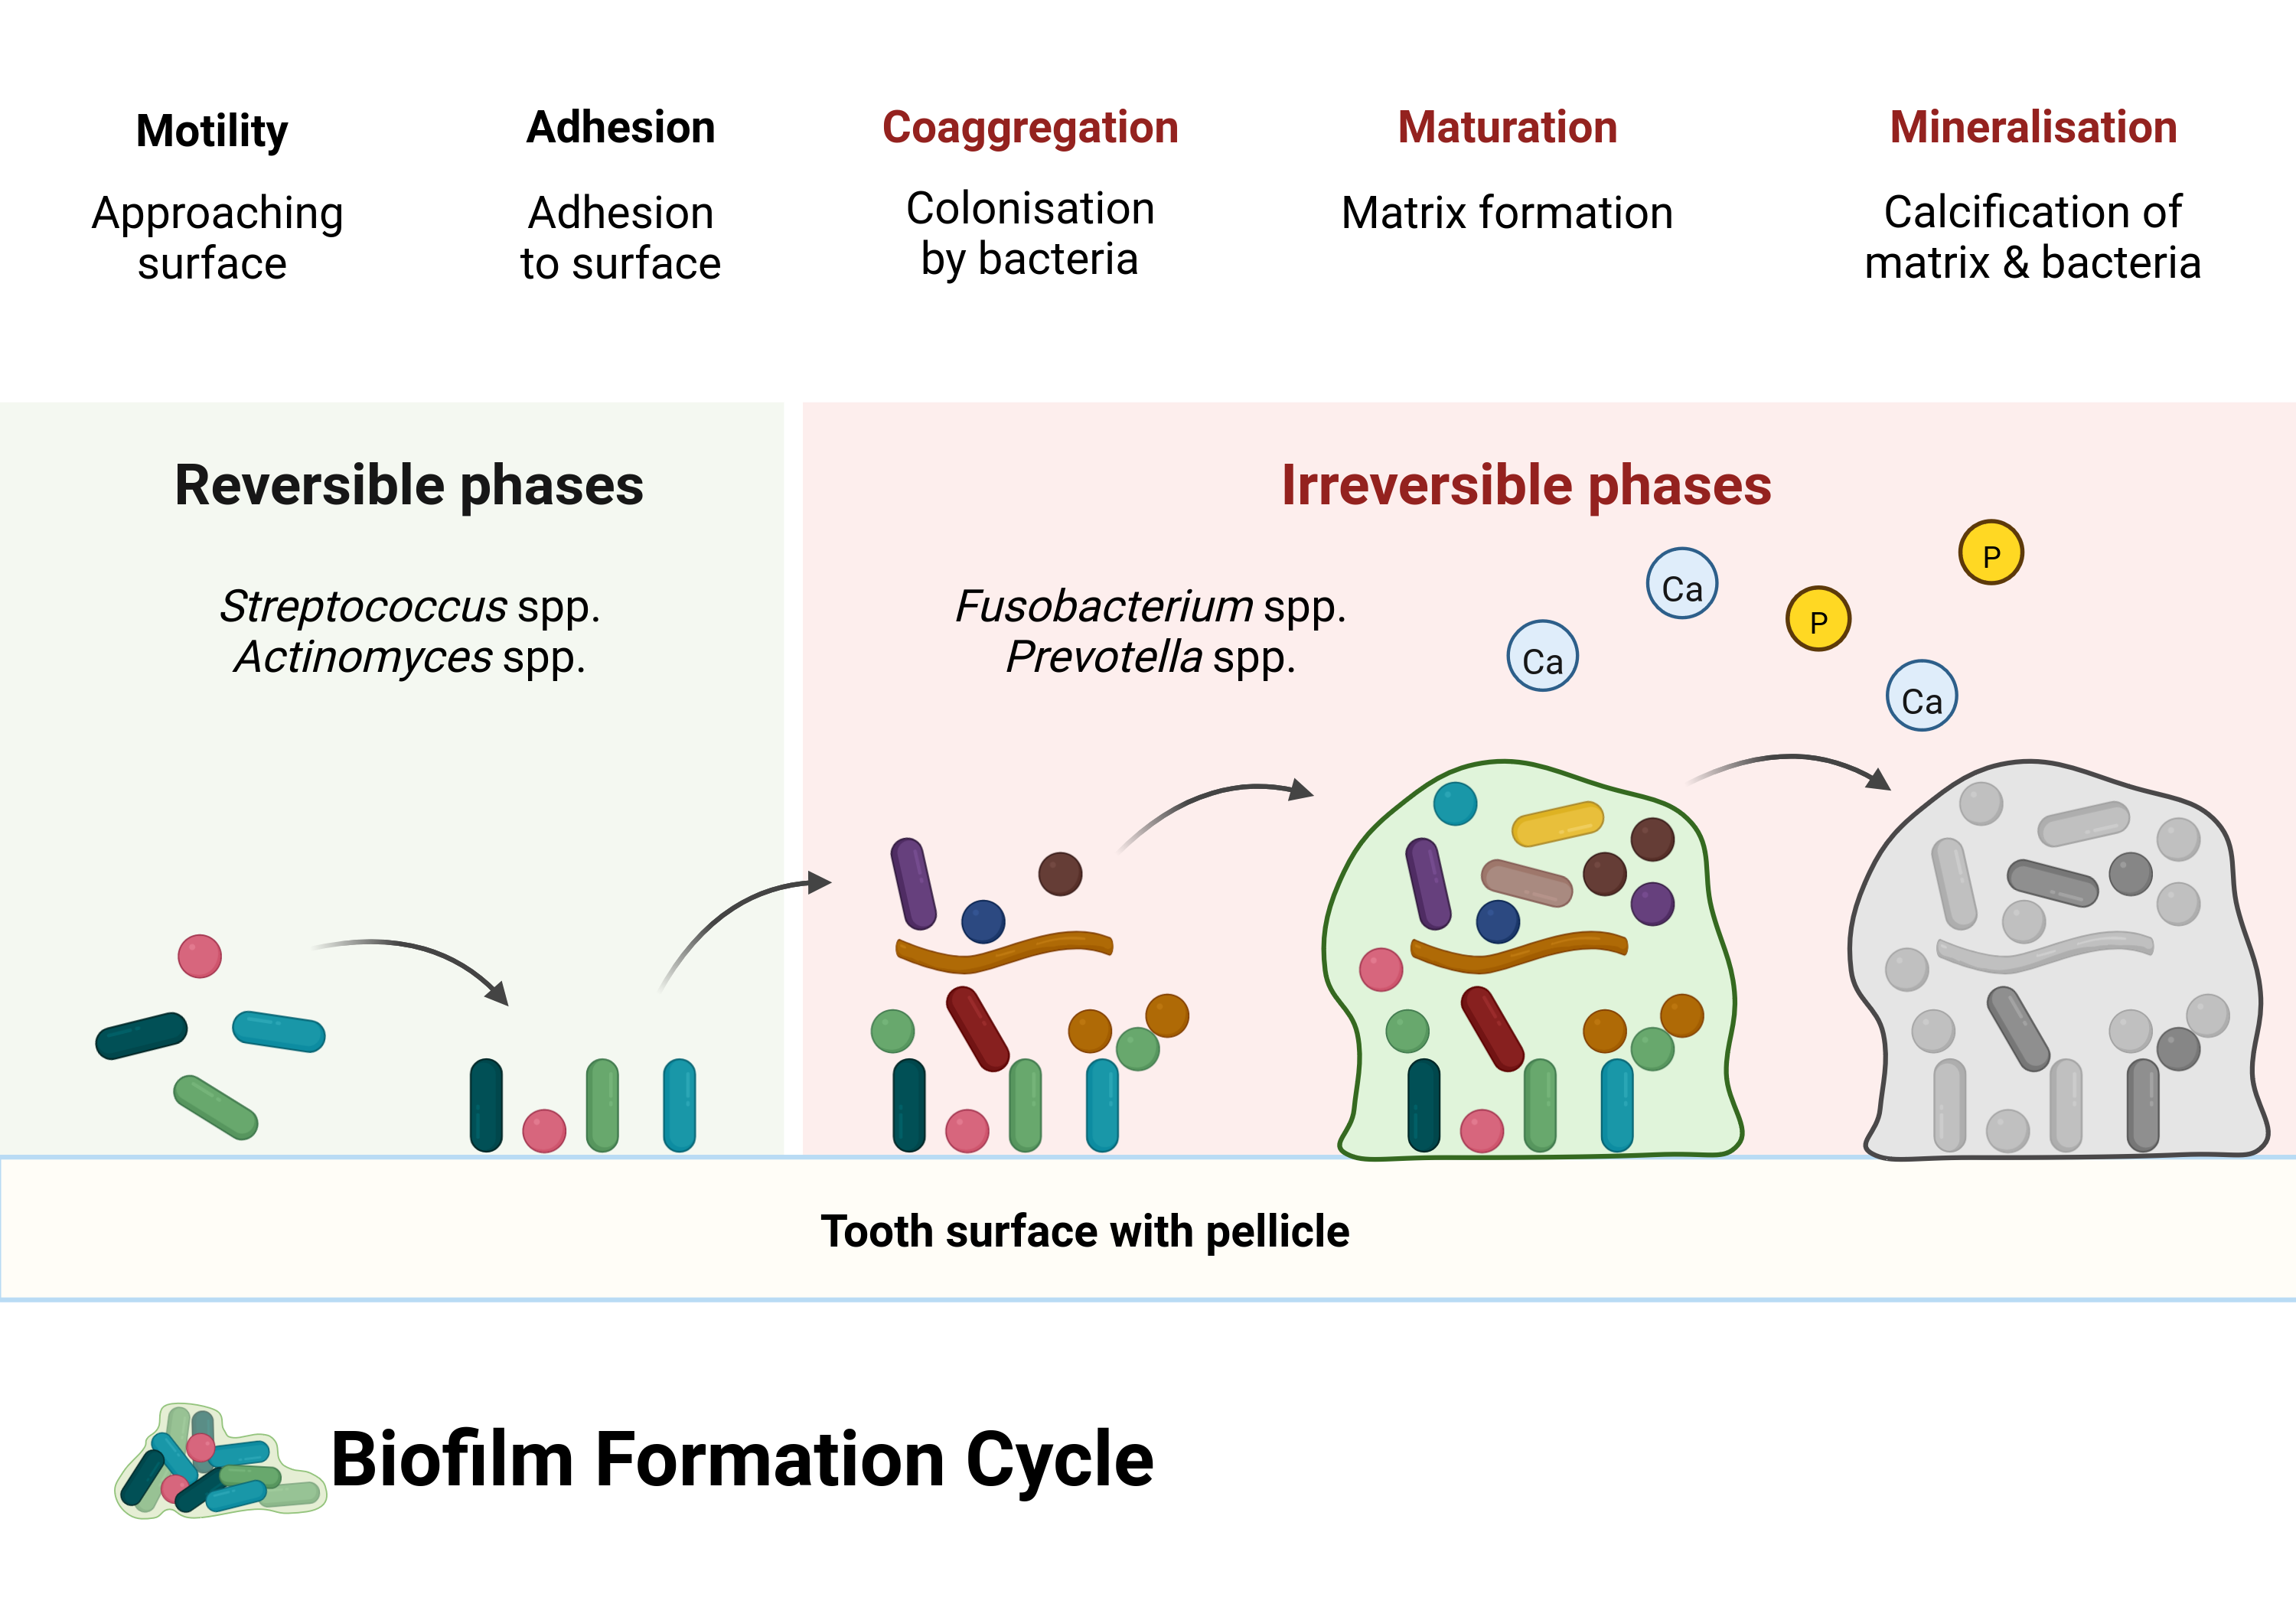
\includegraphics{./figures/biofilm_formation.png}

}

\caption{\label{fig-biofilm-form}A simplified overview of biofilm
formation stages. Created with BioRender.com.}

\end{figure}%

The pellicle contains molecules (known as adhesins) that enable specific
bacteria to attach to complementary receptors on the pellicle, in a
process called adsorption, not to be confused with absorption. The
difference being that it simply attaches to the surface of the tooth
rather than being sucked into the tooth. When the pellicle adheres to
the tooth, it becomes a surface for bacterial attachment
(\citeproc{ref-yaoIdentificationProtein2003}{Yao et al., 2003}). The
first bacteria to attach are known as early coloniser bacteria (or
pioneer colonisers) and include \emph{Streptococcus} species (spp.),
\emph{Actinomyces} spp., and \emph{Haemophilus} spp.
(\citeproc{ref-uzelMicrobialShifts2011}{Uzel et al., 2011};
\citeproc{ref-zijngeBiofilmArchitecture2010}{Zijnge et al., 2010}). The
initial attachment occurs when the random movement of bacteria and the
flow of saliva brings them close enough to the pellicle to attach. Some
bacteria have a limited, often random, ability to move if they have long
tail-like structures known as flagella, but most are brought to the
surface by saliva.

As bacteria approach the pellicle-coated surface of a tooth, there are
both attractive and repulsive forces at work. Repulsion because both the
bacteria and pellicle proteins have a net negative charge
(\citeproc{ref-songEffectsMaterial2015}{Song et al., 2015}), causing
electrostatic repulsive force; and attraction from van der Waals forces.
Bacteria may be more or less likely to attach depending on the distance
from the bacteria to the surface. If the bacteria come too close to the
surface, the initial attraction (primary maximum) will most likely be
overcome by repulsion (primary maximum). Bacteria are more likely to
attach when they encounter attractive forces at a further distance
(secondary minimum), ultimately leading to a game of
`will-they-won't-they' between the bacteria and pellicle. This initial
attachment is a weak physicochemical long-distance (10--20 nm; it's a
long distance for bacteria) attraction; therefore, attachment is
initially reversible, as bacteria can become detached by salivary flow
or shearing action by the tongue
(\citeproc{ref-marshDentalPlaque2016}{Marsh et al., 2016}). This model
of bacterial attachment, also known as the DLVO theory, can partially
explain the aspects involved in microbial adhesion. Further explanation
includes hydrodynamic forces, where hydrophobic components of the
pellicle and cell surface interact
(\citeproc{ref-bosPhysicochemistryInitial1999}{Bos, 1999};
\citeproc{ref-vigeantReversibleIrreversible2002}{Vigeant et al., 2002}).
Overcoming the repulsive forces may be in part facilitated by motility
in some organisms. The aforementioned flagellum, for example, may give
the necessary `push' to reach a region of net attractive forces
(\citeproc{ref-jinSupragingivalCalculus2002}{Jin \& Yip, 2002}).
Additionally, the ionic strength of saliva may play a role in reducing
electrostatic repulsion with increasing ionic strength
(\citeproc{ref-rennerPhysicochemicalRegulation2011}{Renner \& Weibel,
2011}).

\begin{figure}

\centering{

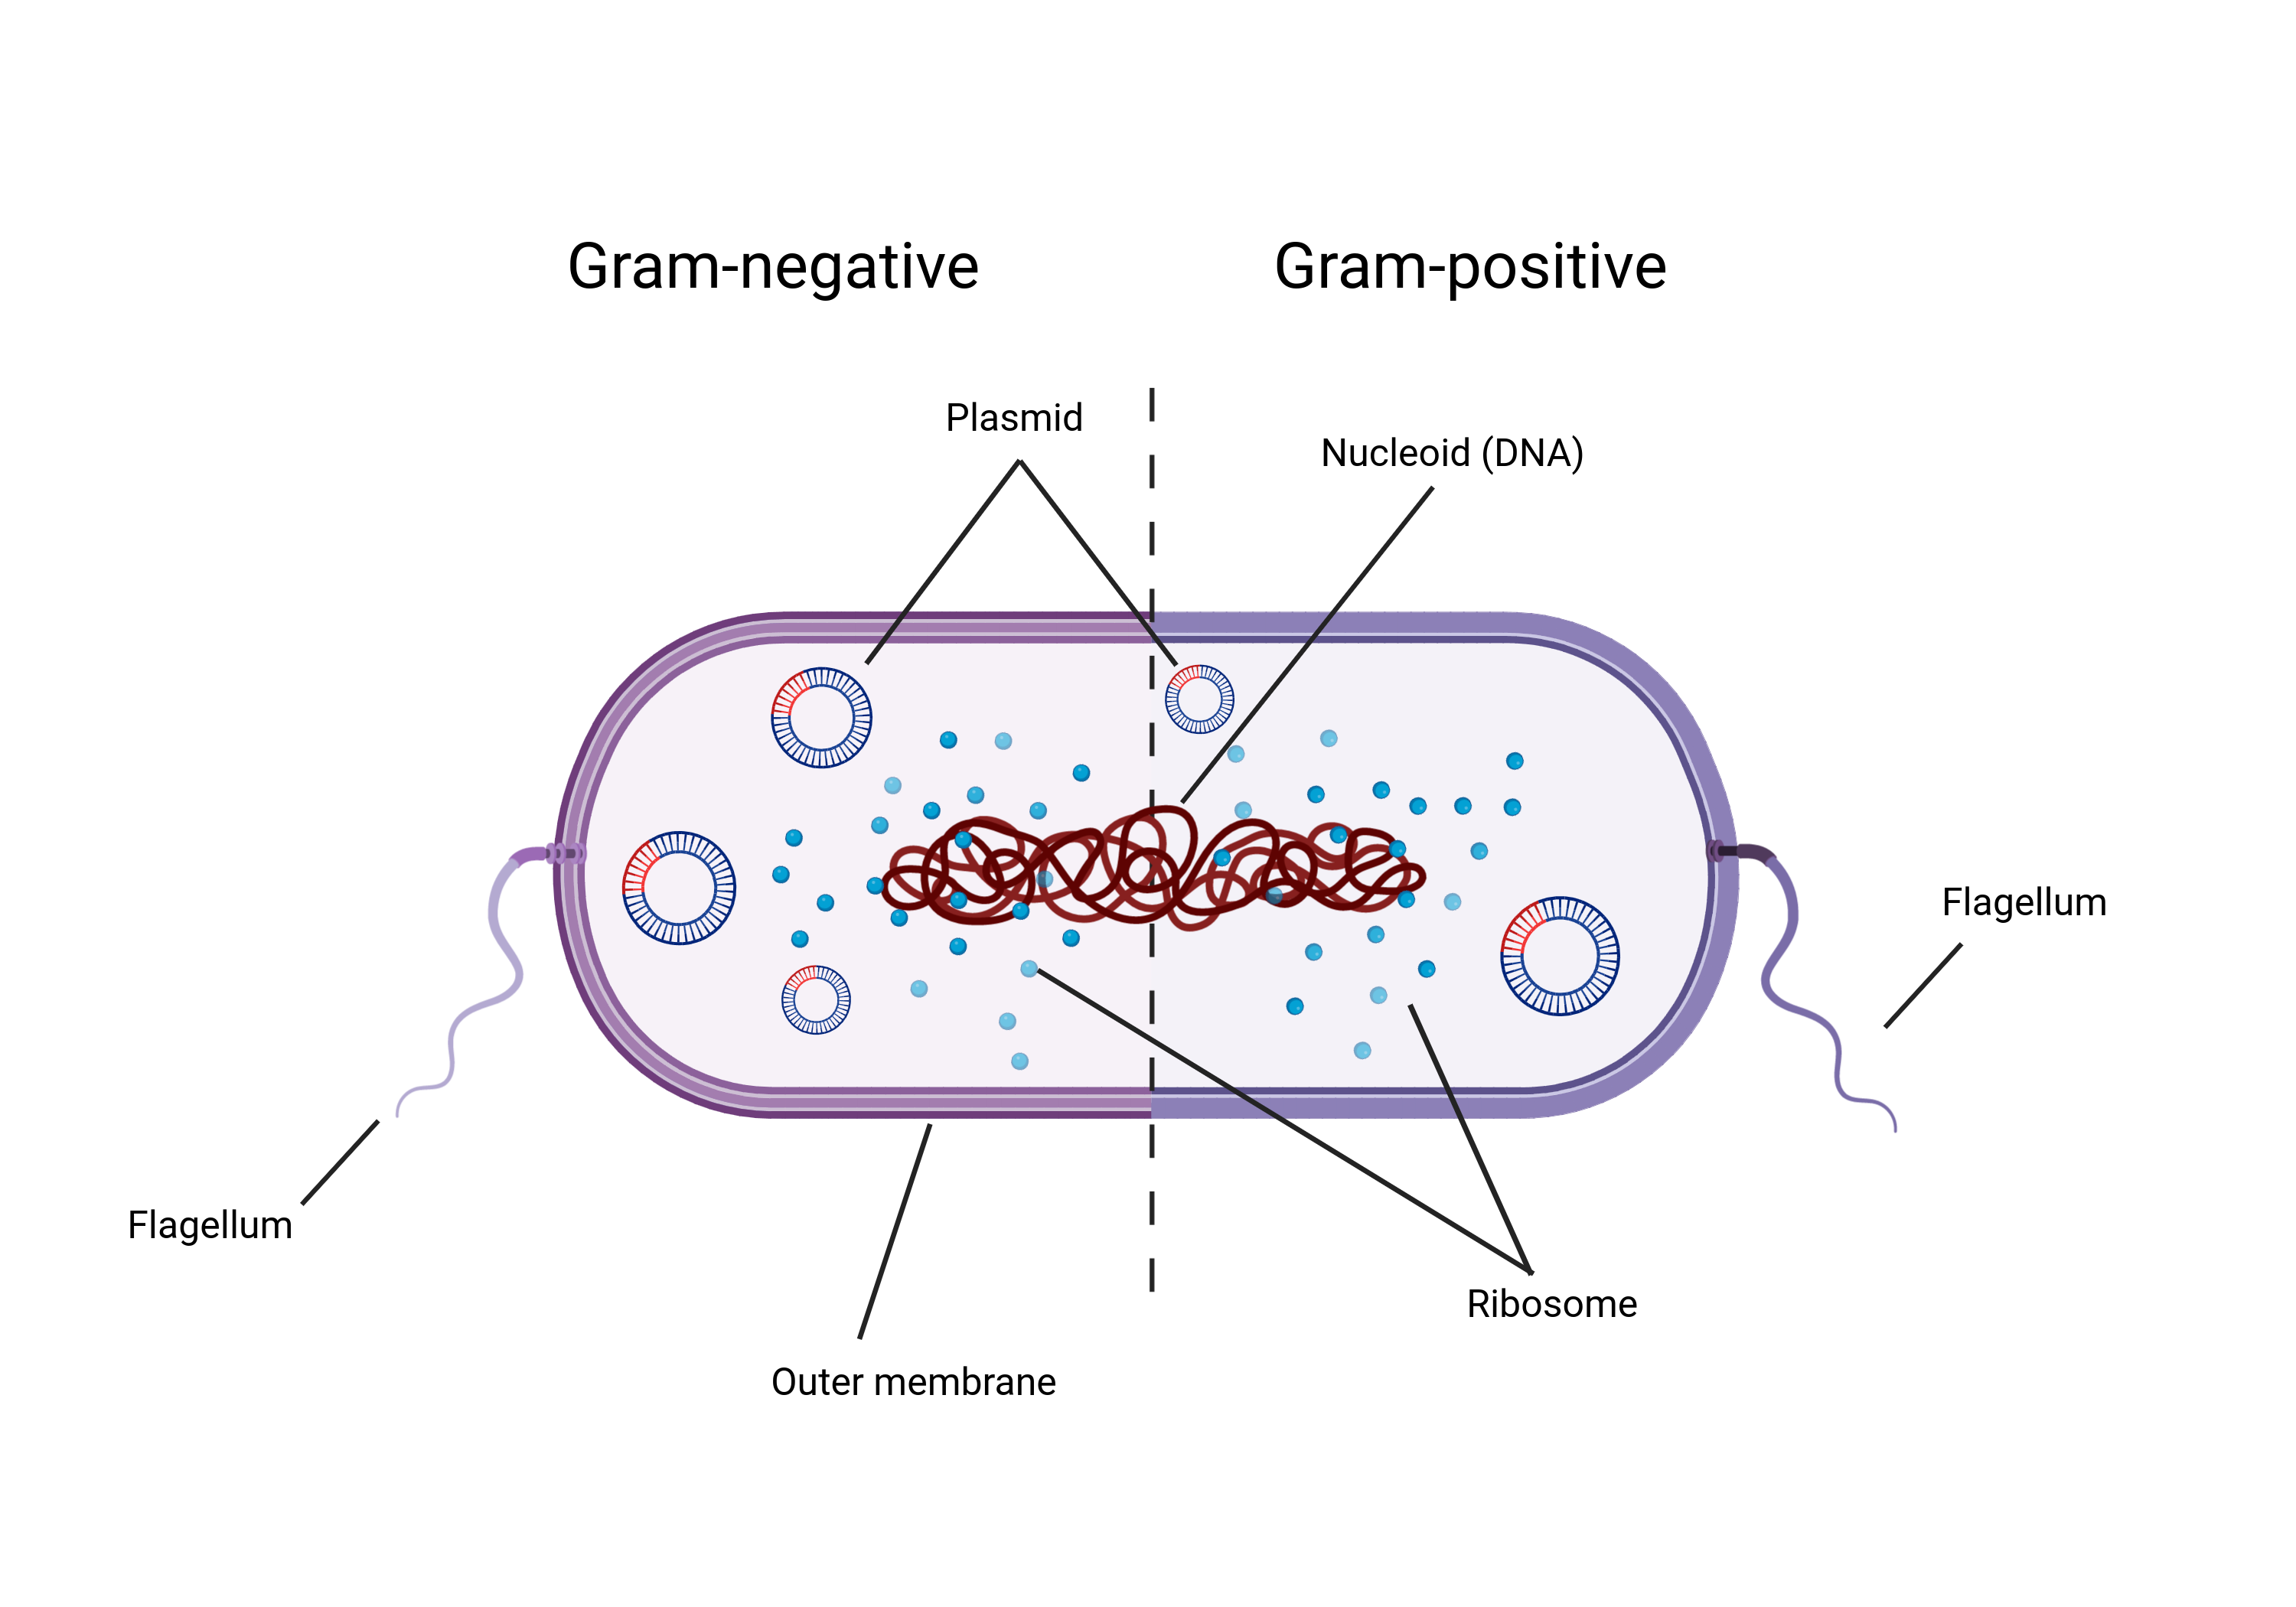
\includegraphics{figures/bacterial-structure.png}

}

\caption{\label{fig-bacterial-structure}General structure of a bacterial
cell. Common features of gram-negative bacteria on the left, and common
features of gram-positive bacteria on the right. Created with
BioRender.com.}

\end{figure}%

Attachment becomes stronger and colonisation becomes more solidified at
a shorter distance, as surface molecules on the bacteria interact with
complementary receptors on the pellicle, and the interactions between
bacteria and pellicle become more direct. Some bacteria have components
on their surface that allow them to attach directly to complementary
components on the dental pellicle (adhesin-receptor interactions). These
attachments are very specific because only certain bacteria have the
right molecules on their surface
(\citeproc{ref-jinSupragingivalCalculus2002}{Jin \& Yip, 2002}). These
receptors are often carbohydrates formed by the host, meaning us. Early
colonisers are also able to attach to proteins and enzymes present in
saliva, as well as onto the surface of other bacteria already attached
to the pellicle (\citeproc{ref-jinSupragingivalCalculus2002}{Jin \& Yip,
2002}; \citeproc{ref-nikitkovaStarchBiofilms2013}{Nikitkova et al.,
2013}). When bacteria come within a shorter distance of the pellicle
they may also attach directly to the surface with other hair-like
structures (fimbriae) that are present on the surface of some bacteria.
These hair-like structures attach to matching receptors that are present
in the pellicle (\citeproc{ref-nobbsStreptococcusAdherence2009}{Nobbs et
al., 2009}).

While some bacteria specialise in attaching to surfaces, not all of them
possess this ability. However, once the specialists have attached, they
facilitate the adhesion of other bacteria (secondary colonisers) by
allowing them to attach to their surface (coadhesion) rather than
directly to the pellicle. For example, \emph{Streptococcus gordonii} can
attach to the pellicle and facilitate coadhesion with \emph{Actinomyces
naeslundii} (\citeproc{ref-palmerCoaggregationInteractions2003}{Palmer
et al., 2003}). Not all attachments involve proteins. They can also
involve carbohydrates, enzymes, and various appendages on the surface of
the bacteria, although these appendages often consist of proteins in
their structure, for example the already mentioned pili and fimbriae
(\citeproc{ref-nobbsStreptococcusAdherence2009}{Nobbs et al., 2009}).
This can occur on a large scale, causing the number and types of
bacteria on the tooth surface to grow, due to the ability of different
species to attach to one another (coaggregation)
(\citeproc{ref-jinSupragingivalCalculus2002}{Jin \& Yip, 2002};
\citeproc{ref-marshDentalPlaque2006}{Marsh, 2006}). Coaggregation and
coadhesion are important parts of the growing oral biofilm. Most taxa
don't have the necessary morphology to attach directly to a substrate,
however most oral taxa CAN coaggregate with other species through
cell-cell interactions, usually involving polysaccharides on the
bacterial-cell surfaces
(\citeproc{ref-kolenbranderOralMultispecies2010}{Kolenbrander et al.,
2010}; \citeproc{ref-palmerInterbacterialAdhesion2017}{Palmer et al.,
2017}).

As the biofilm formed by early colonisers grows through continued
multiplication and coadhesion/coaggregation, the diversity of the
biofilm increases. The proportion of early-colonising streptococci
gradually decreases while there is an increase of \emph{Tannerella
forsythia}, \emph{Actinomyces} spp., and \emph{Fusobacterium nucleatum}
(\citeproc{ref-zijngeBiofilmArchitecture2010}{Zijnge et al., 2010}).
\emph{F. nucleatum} is a bacterium also known as the `bridging species',
as it's believed to play an important part in linking together early and
late coloniser species---including \emph{Prevotella} spp., \emph{S.
gordonii}, and \emph{Porphyromonas gingivalis}--- which might not
otherwise be able to coaggregate
(\citeproc{ref-kolenbranderOralMultispecies2010}{Kolenbrander et al.,
2010}; \citeproc{ref-kolenbranderAdhereToday1993}{Kolenbrander \&
London, 1993}). The increasing diversity of bacteria adhering to a
surface results in communities of bacteria with the ability to
communicate with each other, distribute nutrients, and alter the local
environment for more favourable conditions. This is made possible by the
presence of an extracellular matrix, formed by the production of
polymers by certain bacterial species
(\citeproc{ref-marshMicrobiologyDental2010}{Marsh, 2010}).
Microenvironmental changes can allow species to survive in otherwise
unfavourable environments; for example, the survival of many obligate
anaerobes in an environment which is largely aerobic (oxygen
continuously enters the oral cavity as we breathe). Bacteria with the
ability to consume oxygen and produce carbon dioxide allow bacteria with
a lower oxygen tolerance to thrive
(\citeproc{ref-marshDentalPlaque2005}{Marsh, 2005}). In fact, dental
plaque predominantly consists of obligate and facultative anaerobes and
is especially true for periodontitis-associated biofilms, which tend to
be dominated by more species with a lower oxygen tolerance than their
non-periodontitis counterparts
(\citeproc{ref-curtisRoleMicrobiota2020}{Curtis et al., 2020}). A pH
balance may be maintained by species that are able to consume acidic
metabolic products produced by other species, and convert them to weaker
acids. \emph{Veillonella} spp. especially
(\citeproc{ref-marshDentalPlaque2005}{Marsh, 2005}). Metabolic products
of some bacteria are used by others as nutrients. By-products of urea
metabolism can be used by some organisms, who further break down the
by-products, which can be used by yet other organisms
(\citeproc{ref-flemmingBiofilmsEmergent2016}{Flemming et al., 2016}).
Working as a community can increase survivability in the harsh and
dynamic environment of the oral cavity, with rapid changes in pH,
oxygen, nutrient availability, etc; though, extended fluctuations in
environmental conditions can alter the composition of biofilms
(\citeproc{ref-huangFactorsAssociated2012}{Huang et al., 2012},
\citeproc{ref-huangEffectArginine2017}{2017}).

Perhaps ironically, an important part of the maturation of a biofilm is
the removal of bacteria from the biofilm itself. Removal can occur
through both internal and external mechanisms. It's likely that there is
a continuous loss of microbes near/on the surface of the biofilm caused
by shear forces from saliva and mechanical removal by the tongue. There
can be multiple motivating factors involved in the active detachment by
bacteria, including increasingly adverse conditions within the biofilm,
such as nutrient depletion or an unfavourable local environment. If
sufficiently adverse conditions persist, certain bacteria may make the
active decision to `peace out'. Dispersion of bacteria from a biofilm
requires production of matrix-degrading enzymes, and, as such, not all
bacteria can actively disperse from a biofilm
(\citeproc{ref-petrovaEscapingBiofilm2016}{Petrova \& Sauer, 2016}). The
detached bacteria then colonise other parts of the biofilm, making the
biofilm a highly dynamic structure undergoing continuous remodelling
(\citeproc{ref-flemmingBiofilmsEmergent2016}{Flemming et al., 2016}).

So far, the picture of biofilm formation is one of peaceful
coexsistence, collaboration, and even neighbourly interspecies actions.
A basis for this cooperation is increased overall benefits to the
communities (\citeproc{ref-renduelesMechanismsCompetition2015}{Rendueles
\& Ghigo, 2015}). However, competition between bacteria still exists
within the biofilm. The metabolic by-products produced by some bacteria
may be toxic for others, allowing the producers to gain a competitive
advantage. The aforementioned acid-production by some bacteria can cause
unfavourable conditions for species that prefer more neutral pH
environments, particularly in the absence of the secondary feeders that
would normally neutralise these compounds. A more direct example of
bacterial competition is the ability of bacteria to produce substances
that are toxic to other bacteria. These are often proteins or peptides
termed bacteriocins, and can either inhibit or even kill other bacteria
(\citeproc{ref-dawBacteriocinsNature1996}{Daw \& Falkiner, 1996};
\citeproc{ref-grahamEnterococcusFaecalis2017}{Graham et al., 2017}).
\emph{S. sanguinis} and \emph{S. gordonii} can produce
H\textsubscript{2}O\textsubscript{2} that is toxic to \emph{S. mutans},
a member of their own genus. \emph{S. mutans} can, in turn, produce
mutacin, which inhibits the growth of \emph{S. sorbrinus}. There is no
love lost among these close relatives
(\citeproc{ref-chenSpecificGenes1999}{Chen et al., 1999}). In addition
to H\textsubscript{2}O\textsubscript{2}, oral streptococci can produce
lactate by consuming carbohydrates, giving them a competitive advantage
over acid-sensitive species by altering the local environment. Some
species are resistant to specific metabolic by-products that others
consider toxic, and may even consider them a delicacy (so to speak).
\emph{Veillonella} spp. are an example of organisms that thrive under
these conditions, allowing both streptococci and \emph{Veillonella} spp.
to accumulate in the biofilm and create a favourable environment to
select species (\citeproc{ref-edlundUncoveringComplex2018}{Edlund et
al., 2018}). These are simplistic examples, and often competition
involves more interactions between multiple species taking on various
roles of `sensing', `mediating', and `killing'
(\citeproc{ref-renduelesMechanismsCompetition2015}{Rendueles \& Ghigo,
2015}). Competition between and within species will ultimately shape the
wider biofilm communities.

\subsection{Dental calculus}\label{dental-calculus}

The exact mechanism of dental calculus formation is not fully
understood, but involves processes of biomineralisation and crystal
formation within dental plaque. The main mineral components of calculus
are crystals containing various combinations of calcium and phosphate
ions. Other salts are also present, but the bulk of the crystals are
made up of calcium phosphates. Initial mineralisation of dental plaque
is a chemical process in which equilibrium of minerals in saliva and
gingival crevicular fluid tips towards saturation with regard to calcium
and phosphate, causing an increase of precipitation relative to
dissolution. This means that when the concentration of ions increases
and tips the balance between dissolution and precipitation, salts will
accumulate within and on the surface of the biofilm. An increase in
concentration of minerals within the biofilm reaches a critical
threshold (supersaturation) and nucleation is triggered within the
plaque matrix, initiating crystal growth. This may or may not involve
spontaneous (or homogenous) nucleation, as it's unclear whether mineral
concentrations are sufficient to cause spontaneous nucleation, or
whether other biochemical processes act as a catalyst
(\citeproc{ref-omelonReviewPhosphate2013}{Omelon et al., 2013}). That
it's a chemical process can be shown by the ability to produce calculus
deposits in germ-free rats
(\citeproc{ref-glasBiophysicalStudies1962}{Glas \& Krasse, 1962};
\citeproc{ref-theiladeGermfreeCalculus1964}{Theilade et al., 1964}).
However, it's unclear how the germ-free calculus compares to
conventional calculus, and, to my knowledge there have only been studies
on rats. Just because calculus growth can be induced in sterile
conditions doesn't mean bacteria are not an essential part of the
process. Bacteria are inevitably part of the scaffolding of dental
calculus in humans, since, as I mentioned in the beginning of this
chapter, our mouths are full of bacteria, and dental plaque is
essentially built by bacteria. Mineralisation does seem to start in the
biofilm matrix between microorganisms, but they are eventually also
mineralised along with the biofilm matrix
(\citeproc{ref-friskoppUltrastructureNondecalcified1983}{Friskopp,
1983}). There are pockets of living bacteria within dental calculus.
These pockets and the layer of plaque that covers the surface of dental
calculus are likely what cause the correlation between calculus presence
and periodontal disease (\citeproc{ref-tanBacterialViability2004}{B. T.
K. Tan et al., 2004}). While the process can be explained by chemistry,
the conditions leading up to and surrounding the process are both
chemical and biological in nature, and certainly involve bacteria.

The main source of minerals in the oral cavity is saliva, which enters
the mouth through salivary glands. The three main paired glands are the
parotid, sublingual, and submandibular glands, located by the cheeks,
under the tongue, and under the lower jaw bone, respectively. Saliva
contains sodium (Na), potassium (K), calcium (Ca), chlorine (Cl),
bicarbonate (buffer), and inorganic phosphate (Pi)
(\citeproc{ref-dawesEffectsDiet1970}{Dawes, 1970};
\citeproc{ref-doddsHealthBenefits2005}{Dodds et al., 2005}), and the
locations of the glands contribute to the pattern of dental calculus
deposits within the mouth, which commonly grow on the buccal portion of
maxillary (upper) molars and the lingual portion of mandibular (lower)
incisors (\citeproc{ref-jinSupragingivalCalculus2002}{Jin \& Yip, 2002};
\citeproc{ref-whiteDentalCalculus1997}{White, 1997}). Salivary pH also
affects saturation of salts, which in turn is influenced by salivary
flow rates. Increased flow rate of saliva will increase salivary pH,
which reduces dissolution and increases precipitation of calcium and
phosphate. This is an important mechanism that protects our teeth
against demineralisation of the enamel caused by caries. Protection is
provided by the exchange of calcium and phosphate from saliva to enamel
(\citeproc{ref-dahlenMicrobiologicalStudy2010}{Dahlén et al., 2010}).
Saliva further acts as a buffer for the oral cavity, reducing the impact
of short-term drops in pH caused by metabolic byproducts of
acid-producing bacteria (\citeproc{ref-doddsHealthBenefits2005}{Dodds et
al., 2005}; \citeproc{ref-jinSupragingivalCalculus2002}{Jin \& Yip,
2002}). Higher rates of salivary flow are also likely to contribute to
an increase in calcium and phosphate secretion in addition to pH, all
contributing to an environment favouring plaque mineralisation.
Metabolic byproducts produced by bacteria can also affect local pH, both
pushing towards alkaline conditions as well as acidic. A major cause of
acidic pH is metabolism of overabundant dietary sugars and starch,
especially the metabolic activity of \emph{Streptococcus mutans}, known
to be one of the main culprits behind dental caries
(\citeproc{ref-bowenOralBiofilms2018}{Bowen et al., 2018};
\citeproc{ref-duarteInfluencesStarch2008}{Duarte et al., 2008};
\citeproc{ref-extercateAAA2010}{Exterkate et al., 2010}).

Conversely, alkaline conditions can be generated by metabolism of
various products that can either be directly or indirectly linked to
diet. One such product is urea. Urea is present in saliva, and its
concentration depends on multiple factors. One of these factors is a
high-protein diet, which increases levels of urea in serum and saliva
(\citeproc{ref-lieverseDietAetiology1999}{Lieverse, 1999}). Hydrolysis
of urea produces ammonia and causes a rise in pH. Bacteria possess the
ability to produce ammonia from urea, which is further used by
ammonia-oxidising organisms and converted to nitrite
(\citeproc{ref-flemmingBiofilmsEmergent2016}{Flemming et al., 2016};
\citeproc{ref-sissonsPHResponse1994}{Sissons et al., 1994};
\citeproc{ref-wongCalciumPhosphate2002}{Wong et al., 2002}). In a
similar way, arginine can be broken down to ammonia and increase in pH.
Another pathway to alkalinity is through enzymatic activity. Saliva
contains proteases which specialise in breaking down proteins into
smaller components such as ammonia, and increased protease activity in
saliva may therefore cause an increase in calculus production
(\citeproc{ref-jinSupragingivalCalculus2002}{Jin \& Yip, 2002}).

There are also a number of inhibitors and promoters of mineralisation
present in the oral cavity, originating both from saliva and bacteria.
Substances known to promote plaque mineralisation through hydroxyapatite
formation and deposition, calcium-phospholipid-phosphate complexes
(CPLX), are present in bacteria. \emph{Corynebacterium matruchotii}
(formerly \emph{Bacterionema matruchotii}) accumulates calcium within
its cell structure, and has therefore received a lot of attention in
biomineralisation studies Ennever \& Creamer
(\citeproc{ref-enneverMicrobiologicCalcification1967}{1967}).
Biomineralisation is not a feature unique to \emph{Corynebacterium
matruchotii}. Even species associated with caries may induce
calcification under the right conditions and after cell death
(\citeproc{ref-moorerCalcificationCariogenic1993}{Moorer et al., 1993};
\citeproc{ref-sidawayMicrobiologicalStudy1978a}{Sidaway, 1978}).
Inhibitors of biomineralisation include salivary proline-rich
polypeptides, small amino acids important for the immune system; and
statherin, a protein that controls the precipitation of calcium
phosphate in saliva (\citeproc{ref-jinSupragingivalCalculus2002}{Jin \&
Yip, 2002}).

It's likely that multiple biomineralisation events occur under various
conditions, resulting in a heterogeneous calculus composition with
crystals of various stages of growth
(\citeproc{ref-friskoppUltrastructureNondecalcified1983}{Friskopp,
1983}; \citeproc{ref-friskoppComparativeScanning1980}{Friskopp \&
Hammarström, 1980}). The differing susceptibility of bacteria to
calcification is also a contributor to the heterogeneous composition.
Overall, plaque mineralisation is a complex interaction between
conditions in the local environment, availability of minerals, the
equilibrium between precipitation and dissolution, balance between
nucleation promoters and inhibitors.

\section{Oral biofilm models}\label{background-biofilm-models}

Biofilm models are a way of studying the growth and development of
biofilms. By creating models that replicate the conditions and
complexity (to some extent) of biofilms in a lab, models allow
researchers to conduct various experiments to test the efficacy of
treatments on the growth and pathogenicity of biofilms. There are many
choices to be made when growing a biofilm, such as the composition of
the initial oral microbial community, nutrient content and availability,
and the makeup of the atmosphere in which the model is situated. As
such, biofilm models can differ widely in their complexity and ability
to mimic conditions in a human mouth. A choice of model can be made
based on the end-goals of the research, or in some cases the choice is
made for you based on (a lack of) available equipment and financial
constraints. All models must have a defined biome containing a
substratum and nutrients. The substratum is a surface on which the
biofilm is intended to form and grow. For oral biofilm models the
environment is the oral cavity and the substrata are the teeth, tongue,
mucosa, or whatever the model is the biofilm supposed to be mimicking.
The simplest models generally involve multiwell plates (e.g., 6-, 24-,
and 98-well plates) with a substratum, usually glass cover-slips or
hydroxyapatite discs, placed at the bottom of the well. Similar models
suspend the substrata from a lid to promote active attachment of
bacteria to the substrata (\citeproc{ref-extercateAAA2010}{Exterkate et
al., 2010}). When the substrata are attached to a lid instead of the
multiwell plates, it allows samples to be periodically transferred
between solutions/media if necessary, adding more flexibility to the
experimental setup.

Next, an inoculate is chosen. This can be anything from a single species
of bacterium (pure culture), to multiple select species (defined
consortium), to all organisms occurring naturally within a system
(microcosm) (\citeproc{ref-mcbainBiofilmModels2009}{McBain, 2009}). The
purpose of the inoculate is to initiate biofilm formation by allowing
the bacteria to adsorb to the substrata, ideally in the presence of a
conditioning film, such as saliva. For pure cultures and defined
consortia, the inoculate may come from saliva or another oral site, such
as dental plaque. The bacteria of interest are then isolated using
selective media, essentially providing ideal growing conditions to
certain types of bacteria, promoting their growth and eliminating others
(e.g. \citeproc{ref-bassonEstablishmentCommunity1996}{Basson \& van Wyk,
1996}). Alternatively, the bacteria can be acquired directly from
companies like the American Type Culture Collection (ATCC). For
microcosms, the inoculate is often the saliva itself, or dental plaque,
in its (mostly) raw form. The inoculate is added to the wells to
initiate biofilm formation on the substrata as described
\hyperref[dental-plaque]{above}. As such, the content of the inoculate
influences the complexity of the biofilm microbiome as well as the
interactions between the communities within the biofilm
(\citeproc{ref-roderStudyingBacterial2016}{Røder et al., 2016}). It's
not always possible to use donated saliva as a growth medium for the
duration of the experiment, especially if the experiment lasts more than
a few days. Media with salivary components can be created as a
substitute for long lasting experiments. There are many different
recipes for media floating around out there, but most of them are
generally a mixture containing mucin, proteins, minerals commonly found
in saliva, and a buffer to maintain pH
(\citeproc{ref-extercateAAA2010}{Exterkate et al., 2010};
\citeproc{ref-prattenVitroStudies1998}{Pratten et al., 1998};
\citeproc{ref-shellisSyntheticSaliva1978}{Shellis, 1978};
\citeproc{ref-sissonsMultistationPlaque1991}{Sissons et al., 1991};
\citeproc{ref-tianUsingDGGE2010}{Tian et al., 2010}).

More complicated models make use of increasingly sophisticated equipment
to mimic the oral environment. Another level of model complexity can be
added by adjusting the rate at which nutrients are dispersed through the
system, and the overall nutrient supply. Nutrient distribution can be
continuous, semi-continuous, or batch cultures, with the latter
providing a finite amount of nutrients in a closed system. An example of
a batch culture model is a biofilm grown on an agar plate, which has a
finite amount of resources
(\citeproc{ref-kearnsMasterRegulator2005}{Kearns et al., 2005}). Once
the nutrients in the agar have been depleted, that's it. At the other
end of the spectrum is a system with a pump attached to a reservoir that
can continuously supply the biofilm with growth medium, similar to
salivary flow. In between the former options is the semi-continuous
supply of nutrients. This can, for example, be the multiwell plate model
with a lid, where the samples can be periodically transferred to new
plates containing fresh growth medium
(\citeproc{ref-extercateAAA2010}{Exterkate et al., 2010}). Other
parameters that can be controlled to more closely simulate conditions in
the oral cavity are pH and gas phase, as can be done with the
multistation artificial mouth. This system gives researchers control
over a large number of parameters using multiple chambers with complete
control over the flow of treatment and/or nutrient
conditions---environmental conditions such as pH, temperature, and gas
phase---and access to real-time measurements
(\citeproc{ref-sissonsArtificialPlaque1997}{Sissons, 1997}).

The duration of an experiment depends on the scope of the study. If the
purpose is to learn more about initial biofilm formation and prevention,
it may only be necessary to grow the biofilms for a few hours to 48
hours (\citeproc{ref-dibdinDiffusionSugars1981}{Dibdin, 1981};
\citeproc{ref-extercateAAA2010}{Exterkate et al., 2010}). If, instead,
the goal is to learn more about biofilm maturation and calcification,
the experiments can run for days or even weeks
(\citeproc{ref-filocheFluorescenceAssay2007}{Filoche et al., 2007};
\citeproc{ref-sissonsMultistationPlaque1991}{Sissons et al., 1991};
\citeproc{ref-wongCalciumPhosphate2002}{Wong et al., 2002}).

Models developed for studying oral biofilms include, in increasing
complexity, the ACTA active attachment model
(\citeproc{ref-extercateAAA2010}{Exterkate et al., 2010}), Calgary
biofilm device (\citeproc{ref-ceriCalgaryBiofilm1999}{Ceri et al.,
1999}), modified Robbins device
(\citeproc{ref-honraetModifiedRobbins2006}{Honraet \& Nelis, 2006}),
constant depth film-fermenter
(\citeproc{ref-petersConstantDepth1988}{Peters \& Wimpenny, 1988}), and
the multistation artificial mouth
(\citeproc{ref-sissonsMultistationPlaque1991}{Sissons et al., 1991})
representing the upper echelon of complexity. Summaries of biofilm
models, including benefits and limitations of the various types, can be
found in reviews by McBain -McBain
(\citeproc{ref-mcbainBiofilmModels2009}{2009}), Tan and colleagues -C.
H. Tan et al. (\citeproc{ref-tanAllTogether2017}{2017}), and Røder and
colleagues -Røder et al.
(\citeproc{ref-roderStudyingBacterial2016}{2016}).

It might be tempting to think that the goal should always be to mimic
the oral environment as closely as possible. However, there are benefits
to more simplistic models, as well as limitations to the more
sophisticated models. Benefits of pure cultures and defined consortia
are reproducibility between experiments and more control over
physiological and factors and making it easier to take various
measurements. Microcosms have the benefit of more closely mimicking the
complexity of the organisms' natural environment
(\citeproc{ref-mcbainBiofilmModels2009}{McBain, 2009}). However, even
microcosms can be limited in their ability to recreate the complexity
and diversity of the oral microbiome
(\citeproc{ref-tianUsingDGGE2010}{Tian et al., 2010}). Alternatives to
\emph{in vitro} models are \emph{in situ} models which usually involve
growing plaque on a removable surface inside the mouth of a willing
participant. These models add a level of realism, as they are grown
inside an actual oral cavity, and can reflect biogeographical
differences in biofilm composition caused by differing conditions across
the oral cavity. They also come with additional difficulties and reduced
control over experimental parameters
(\citeproc{ref-marshRoleMicrobiology1995}{Marsh, 1995};
\citeproc{ref-zeroSituCaries1995}{Zero, 1995}).

Reiterating a point made in the \hyperref[chap-intro]{Introduction}, and
\hyperref[chap-discussion]{Discussion}, and probably somewhere in the
articles as well, the benefit of using an oral biofilm model over
naturally occurring dental calculus in the mouth of a research
participant, is the control that it provides to tweak every aspect of
the system, from the quantity and quality of nutrients available, to the
amount of enzymes and bacterial species present. Plus, the added ethical
benefit of not needing to ask someone to give up their oral hygiene
regime for a few weeks. The following chapters,
\hyperref[byoc-valid]{Chapter 3} and \hyperref[byoc-starch]{Chapter 4},
provide a small glimpse of what a model looks like, and how it might be
used to inform archaeological research.

\section*{References cited}\label{references-cited-1}
\addcontentsline{toc}{section}{References cited}

\markright{References cited}

\phantomsection\label{refs-2}
\begin{CSLReferences}{1}{0}
\bibitem[\citeproctext]{ref-bassonEstablishmentCommunity1996}
Basson, N. J., \& van Wyk, C. W. (1996). The establishment of a
community of oral bacteria that controls the growth of {Candida}
albicans in a chemostat. \emph{Oral Microbiology and Immunology},
\emph{11}(3), 199--202.
\url{https://doi.org/10.1111/j.1399-302X.1996.tb00358.x}

\bibitem[\citeproctext]{ref-bosPhysicochemistryInitial1999}
Bos, R. (1999). Physico-chemistry of initial microbial adhesive
interactions \textendash{} its mechanisms and methods for study.
\emph{FEMS Microbiology Reviews}, \emph{23}(2), 179--229.
\url{https://doi.org/10.1016/S0168-6445(99)00004-2}

\bibitem[\citeproctext]{ref-bowenOralBiofilms2018}
Bowen, W. H., Burne, R. A., Wu, H., \& Koo, H. (2018). Oral {Biofilms}:
{Pathogens}, {Matrix} and {Polymicrobial Interactions} in
{Microenvironments}. \emph{Trends in Microbiology}, \emph{26}(3),
229--242. \url{https://doi.org/10.1016/j.tim.2017.09.008}

\bibitem[\citeproctext]{ref-boyan-salyersRelationshipProteolipids1980}
Boyan-Salyers, B. D., \& Boskey, A. L. (1980). Relationship between
proteolipids and calcium-phospholipid-phosphate complexes
{inBacterionema} matruchotii calcification. \emph{Calcified Tissue
International}, \emph{30}(1), 167--174.
\url{https://doi.org/10.1007/BF02408622}

\bibitem[\citeproctext]{ref-ceriCalgaryBiofilm1999}
Ceri, H., Olson, M. E., Stremick, C., Read, R. R., Morck, D., \& Buret,
A. (1999). The {Calgary Biofilm Device}: {New Technology} for {Rapid
Determination} of {Antibiotic Susceptibilities} of {Bacterial Biofilms}.
\emph{Journal of Clinical Microbiology}, \emph{37}(6), 1771--1776.
\url{https://doi.org/10.1128/JCM.37.6.1771-1776.1999}

\bibitem[\citeproctext]{ref-chenSpecificGenes1999}
Chen, P., Qi, F., Novak, J., \& Caufield, P. W. (1999).
\href{https://www.ncbi.nlm.nih.gov/pmc/articles/PMC91190}{The {Specific
Genes} for {Lantibiotic Mutacin II Biosynthesis} in {Streptococcus}
mutans {T8 Are Clustered} and {Can Be} {Transferred En Bloc}}.
\emph{Applied and Environmental Microbiology}, \emph{65}(3), 1356--1360.

\bibitem[\citeproctext]{ref-costertonBacterialBiofilms1987}
Costerton, J. W., Cheng, K. J., Geesey, G. G., Ladd, T. I., Nickel, J.
C., Dasgupta, M., \& Marrie, T. J. (1987). Bacterial {Biofilms} in
{Nature} and {Disease}. \emph{Annual Review of Microbiology},
\emph{41}(1), 435--464.
\url{https://doi.org/10.1146/annurev.mi.41.100187.002251}

\bibitem[\citeproctext]{ref-costertonMicrobialBiofilms1995}
Costerton, J. W., Lewandowski, Z., Caldwell, D. E., Korber, D. R., \&
Lappin-Scott, H. M. (1995). Microbial {Biofilms}. \emph{Annual Review of
Microbiology}, \emph{49}(1), 711--745.
\url{https://doi.org/10.1146/annurev.mi.49.100195.003431}

\bibitem[\citeproctext]{ref-curtisRoleMicrobiota2020}
Curtis, M. A., Diaz, P. I., \& Dyke, T. E. V. (2020). The role of the
microbiota in periodontal disease. \emph{Periodontology 2000},
\emph{83}(1), 14--25. \url{https://doi.org/10.1111/prd.12296}

\bibitem[\citeproctext]{ref-dahlenMicrobiologicalStudy2010}
Dahlén, G., Konradsson, K., Eriksson, S., Teanpaisan, R., Piwat, S., \&
Carlén, A. (2010). A microbiological study in relation to the presence
of caries and calculus. \emph{Acta Odontologica Scandinavica},
\emph{68}(4), 199--206. \url{https://doi.org/10.3109/00016351003745514}

\bibitem[\citeproctext]{ref-dawBacteriocinsNature1996}
Daw, M. A., \& Falkiner, F. R. (1996). Bacteriocins: Nature, function
and structure. \emph{Micron (Oxford, England: 1993)}, \emph{27}(6),
467--479. \url{https://doi.org/10.1016/s0968-4328(96)00028-5}

\bibitem[\citeproctext]{ref-dawesEffectsDiet1970}
Dawes, C. (1970). Effects of {Diet} on {Salivary Secretion} and
{Composition}. \emph{Journal of Dental Research}, \emph{49}, 1263--1272.

\bibitem[\citeproctext]{ref-dibdinDiffusionSugars1981}
Dibdin, G. H. (1981). Diffusion of sugars and carboxylic acids through
human dental plaque in vitro. \emph{Archives of Oral Biology},
\emph{26}(6), 515--523.
\url{https://doi.org/10.1016/0003-9969(81)90010-8}

\bibitem[\citeproctext]{ref-doddsHealthBenefits2005}
Dodds, M. W. J., Johnson, D. A., \& Yeh, C.-K. (2005). Health benefits
of saliva: A review. \emph{Journal of Dentistry}, \emph{33}(3),
223--233. \url{https://doi.org/10.1016/j.jdent.2004.10.009}

\bibitem[\citeproctext]{ref-duarteInfluencesStarch2008}
Duarte, S., Klein, M. I., Aires, C. P., Cury, J. A., Bowen, W. H., \&
Koo, H. (2008). Influences of starch and sucrose on {Streptococcus}
mutans biofilms. \emph{Oral Microbiology and Immunology}, \emph{23}(3),
206--212. \url{https://doi.org/10.1111/j.1399-302X.2007.00412.x}

\bibitem[\citeproctext]{ref-edlundUncoveringComplex2018}
Edlund, A., Yang, Y., Yooseph, S., He, X., Shi, W., \& McLean, J. S.
(2018). Uncovering complex microbiome activities via metatranscriptomics
during 24 hours of oral biofilm assembly and maturation.
\emph{Microbiome}, \emph{6}(1), 217.
\url{https://doi.org/10.1186/s40168-018-0591-4}

\bibitem[\citeproctext]{ref-enneverIntracellularCalcification1960}
Ennever, J. (1960). Intracellular {Calcification} by {Oral Filamentous
Microorganisms}. \emph{The Journal of Periodontology}, \emph{31}(4),
304--307. \url{https://doi.org/10.1902/jop.1960.31.4.304}

\bibitem[\citeproctext]{ref-enneverMicrobiologicCalcification1967}
Ennever, J., \& Creamer, H. (1967). Microbiologic calcification: {Bone}
mineral and bacteria. \emph{Calcified Tissue Research}, \emph{1}(1),
87--93. \url{https://doi.org/10.1007/BF02008078}

\bibitem[\citeproctext]{ref-extercateAAA2010}
Exterkate, R. A. M., Crielaard, W., \& Ten Cate, J. M. (2010). Different
{Response} to {Amine Fluoride} by {Streptococcus} mutans and
{Polymicrobial Biofilms} in a {Novel High-Throughput Active Attachment
Model}. \emph{Caries Research}, \emph{44}(4), 372--379.
\url{https://doi.org/10.1159/000316541}

\bibitem[\citeproctext]{ref-filocheFluorescenceAssay2007}
Filoche, S. K., Coleman, M. J., Angker, L., \& Sissons, C. H. (2007). A
fluorescence assay to determine the viable biomass of microcosm dental
plaque biofilms. \emph{Journal of Microbiological Methods},
\emph{69}(3), 489--496.
\url{https://doi.org/10.1016/j.mimet.2007.02.015}

\bibitem[\citeproctext]{ref-flemmingBiofilmsEmergent2016}
Flemming, H.-C., Wingender, J., Szewzyk, U., Steinberg, P., Rice, S. A.,
\& Kjelleberg, S. (2016). Biofilms: An emergent form of bacterial life.
\emph{Nature Reviews Microbiology}, \emph{14}(9), 563--575.
\url{https://doi.org/10.1038/nrmicro.2016.94}

\bibitem[\citeproctext]{ref-friskoppUltrastructureNondecalcified1983}
Friskopp, J. (1983). Ultrastructure of {Nondecalcified Supragingival}
and {Subgingival Calculus}. \emph{Journal of Periodontology},
\emph{54}(9), 542--550. \url{https://doi.org/10.1902/jop.1983.54.9.542}

\bibitem[\citeproctext]{ref-friskoppComparativeScanning1980}
Friskopp, J., \& Hammarström, L. (1980). A {Comparative}, {Scanning
Electron Microscopic Study} of {Supragingival} and {Subgingival
Calculus}. \emph{Journal of Periodontology}, \emph{51}(10), 553--562.
\url{https://doi.org/10.1902/jop.1980.51.10.553}

\bibitem[\citeproctext]{ref-glasBiophysicalStudies1962}
Glas, J.-E., \& Krasse, B. (1962). Biophysical {Studies} on {Dental
Calculus} from {Germfree} and {Conventional Rats}. \emph{Acta
Odontologica Scandinavica}, \emph{20}(2), 127--134.
\url{https://doi.org/10.3109/00016356209026100}

\bibitem[\citeproctext]{ref-grahamEnterococcusFaecalis2017}
Graham, C. E., Cruz, M. R., Garsin, D. A., \& Lorenz, M. C. (2017).
Enterococcus faecalis bacteriocin {EntV} inhibits hyphal morphogenesis,
biofilm formation, and virulence of {Candida} albicans.
\emph{Proceedings of the National Academy of Sciences}, \emph{114}(17),
4507--4512. \url{https://doi.org/10.1073/pnas.1620432114}

\bibitem[\citeproctext]{ref-honraetModifiedRobbins2006}
Honraet, K., \& Nelis, H. J. (2006). Use of the modified robbins device
and fluorescent staining to screen plant extracts for the inhibition of
{S}. Mutans biofilm formation. \emph{Journal of Microbiological
Methods}, \emph{64}(2), 217--224.
\url{https://doi.org/10.1016/j.mimet.2005.05.005}

\bibitem[\citeproctext]{ref-huangFactorsAssociated2012}
Huang, X., Exterkate, R. A. M., \& ten Cate, J. M. (2012). Factors
{Associated} with {Alkali Production} from {Arginine} in {Dental
Biofilms}. \emph{Journal of Dental Research}, \emph{91}(12), 1130--1134.
\url{https://doi.org/10.1177/0022034512461652}

\bibitem[\citeproctext]{ref-huangEffectArginine2017}
Huang, X., Zhang, K., Deng, M., Exterkate, R. A. M., Liu, C., Zhou, X.,
Cheng, L., \& ten Cate, J. M. (2017). Effect of arginine on the growth
and biofilm formation of oral bacteria. \emph{Archives of Oral Biology},
\emph{82}, 256--262.
\url{https://doi.org/10.1016/j.archoralbio.2017.06.026}

\bibitem[\citeproctext]{ref-jinSupragingivalCalculus2002}
Jin, Y., \& Yip, H.-K. (2002). Supragingival {Calculus}: {Formation} and
{Control}. \emph{Critical Reviews in Oral Biology \& Medicine}.
\url{https://doi.org/10.1177/154411130201300506}

\bibitem[\citeproctext]{ref-kearnsMasterRegulator2005}
Kearns, D. B., Chu, F., Branda, S. S., Kolter, R., \& Losick, R. (2005).
A master regulator for biofilm formation by {Bacillus} subtilis.
\emph{Molecular Microbiology}, \emph{55}(3), 739--749.
\url{https://doi.org/10.1111/j.1365-2958.2004.04440.x}

\bibitem[\citeproctext]{ref-kolenbranderAdhereToday1993}
Kolenbrander, P. E., \& London, J. (1993). Adhere today, here tomorrow:
Oral bacterial adherence. \emph{Journal of Bacteriology},
\emph{175}(11), 3247--3252.
\url{https://doi.org/10.1128/jb.175.11.3247-3252.1993}

\bibitem[\citeproctext]{ref-kolenbranderOralMultispecies2010}
Kolenbrander, P. E., Palmer, R. J., Periasamy, S., \& Jakubovics, N. S.
(2010). Oral multispecies biofilm development and the key role of
cell\textendash cell distance. \emph{Nature Reviews Microbiology},
\emph{8}(7), 471--480. \url{https://doi.org/10.1038/nrmicro2381}

\bibitem[\citeproctext]{ref-lieverseDietAetiology1999}
Lieverse, A. R. (1999). Diet and the aetiology of dental calculus.
\emph{International Journal of Osteoarchaeology}, \emph{9}(4), 219--232.
\url{https://doi.org/10.1002/(SICI)1099-1212(199907/08)9:4\%3C219::AID-OA475\%3E3.0.CO;2-V}

\bibitem[\citeproctext]{ref-marshRoleMicrobiology1995}
Marsh, P. D. (1995). The {Role} of {Microbiology} in {Models} of {Dental
Caries}. \emph{Advances in Dental Research}, \emph{9}(3), 244--254.
\url{https://doi.org/10.1177/08959374950090030901}

\bibitem[\citeproctext]{ref-marshDentalPlaque2005}
Marsh, P. D. (2005). Dental plaque: Biological significance of a biofilm
and community life-style. \emph{Journal of Clinical Periodontology},
\emph{32}(s6), 7--15.
\url{https://doi.org/10.1111/j.1600-051X.2005.00790.x}

\bibitem[\citeproctext]{ref-marshDentalPlaque2006}
Marsh, P. D. (2006). Dental plaque as a biofilm and a microbial
community \textendash{} implications for health and disease. \emph{BMC
Oral Health}, \emph{6}(S1), S14.
\url{https://doi.org/10.1186/1472-6831-6-S1-S14}

\bibitem[\citeproctext]{ref-marshMicrobiologyDental2010}
Marsh, P. D. (2010). Microbiology of {Dental Plaque Biofilms} and {Their
Role} in {Oral Health} and {Caries}. \emph{Dental Clinics of North
America}, \emph{54}(3), 441--454.
\url{https://doi.org/10.1016/j.cden.2010.03.002}

\bibitem[\citeproctext]{ref-marshPhysiologicalApproaches1997}
Marsh, P. D., \& Bradshaw, D. J. (1997). Physiological {Approaches} to
the {Control} of {Oral Biofilms}. \emph{Advances in Dental Research},
\emph{11}(1), 176--185.
\url{https://doi.org/10.1177/08959374970110010901}

\bibitem[\citeproctext]{ref-marshDentalPlaque2016}
Marsh, P. D., Lewis, M. A. O., Rogers, H., Williams, D. W., \& Wilson,
M. (2016). Dental {Plaque}. In \emph{Marsh and {Martin}'s {Oral
Microbiology}} (6th Edition, pp. 81--111). {Elsevier Health Sciences}.

\bibitem[\citeproctext]{ref-mcbainBiofilmModels2009}
McBain, A. J. (2009). In {Vitro Biofilm Models}: {An Overview}. In
\emph{Advances in {Applied Microbiology}} (Vol. 69, pp. 99--132).
{Academic Press}. \url{https://doi.org/10.1016/S0065-2164(09)69004-3}

\bibitem[\citeproctext]{ref-moorerCalcificationCariogenic1993}
Moorer, W. R., Ten Cate, J. M., \& Buijs, J. F. (1993). Calcification of
a {Cariogenic Streptococcus} and of {Corynebacterium} ({Bacterionema})
matruchotii. \emph{Journal of Dental Research}, \emph{72}(6),
1021--1026. \url{https://doi.org/10.1177/00220345930720060501}

\bibitem[\citeproctext]{ref-nikitkovaStarchBiofilms2013}
Nikitkova, A. E., Haase, E. M., \& Scannapieco, F. A. (2013). Taking the
{Starch} out of {Oral Biofilm Formation}: {Molecular Basis} and
{Functional Significance} of {Salivary} {\(\alpha\)}-{Amylase Binding}
to {Oral Streptococci}. \emph{Applied and Environmental Microbiology},
\emph{79}(2), 416--423. \url{https://doi.org/10.1128/AEM.02581-12}

\bibitem[\citeproctext]{ref-nobbsStreptococcusAdherence2009}
Nobbs, A. H., Lamont, R. J., \& Jenkinson, H. F. (2009). Streptococcus
{Adherence} and {Colonization}. \emph{Microbiology and Molecular Biology
Reviews}, \emph{73}(3), 407--450.
\url{https://doi.org/10.1128/MMBR.00014-09}

\bibitem[\citeproctext]{ref-omelonReviewPhosphate2013}
Omelon, S., Ariganello, M., Bonucci, E., Grynpas, M., \& Nanci, A.
(2013). A {Review} of {Phosphate Mineral Nucleation} in {Biology} and
{Geobiology}. \emph{Calcified Tissue International}, \emph{93}(4),
382--396. \url{https://doi.org/10.1007/s00223-013-9784-9}

\bibitem[\citeproctext]{ref-palmerCoaggregationInteractions2003}
Palmer, R. J., Gordon, S. M., Cisar, J. O., \& Kolenbrander, P. E.
(2003). Coaggregation-{Mediated Interactions} of {Streptococci} and
{Actinomyces Detected} in {Initial Human Dental Plaque}. \emph{Journal
of Bacteriology}, \emph{185}(11), 3400--3409.
\url{https://doi.org/10.1128/JB.185.11.3400-3409.2003}

\bibitem[\citeproctext]{ref-palmerInterbacterialAdhesion2017}
Palmer, R. J., Shah, N., Valm, A., Paster, B., Dewhirst, F., Inui, T.,
\& Cisar, J. O. (2017). Interbacterial {Adhesion Networks} within {Early
Oral Biofilms} of {Single Human Hosts}. \emph{Applied and Environmental
Microbiology}, \emph{83}(11), e00407--17.
\url{https://doi.org/10.1128/AEM.00407-17}

\bibitem[\citeproctext]{ref-petersConstantDepth1988}
Peters, A., \& Wimpenny, J. W. T. (1988). A {Constant-Depth Laboratory
Model Film Fermenter}. In \emph{{CRC Handbook} of {Laboratory Model
Systems} for {Microbial Ecosystems}}. {CRC Press}.

\bibitem[\citeproctext]{ref-petersonViscoelasticityBiofilms2015}
Peterson, B. W., He, Y., Ren, Y., Zerdoum, A., Libera, M. R., Sharma, P.
K., van Winkelhoff, A.-J., Neut, D., Stoodley, P., van der Mei, H. C.,
\& Busscher, H. J. (2015). Viscoelasticity of biofilms and their
recalcitrance to mechanical and chemical challenges. \emph{FEMS
Microbiology Reviews}, \emph{39}(2), 234--245.
\url{https://doi.org/10.1093/femsre/fuu008}

\bibitem[\citeproctext]{ref-petrovaEscapingBiofilm2016}
Petrova, O. E., \& Sauer, K. (2016). Escaping the biofilm in more than
one way: Desorption, detachment or dispersion. \emph{Current Opinion in
Microbiology}, \emph{30}, 67--78.
\url{https://doi.org/10.1016/j.mib.2016.01.004}

\bibitem[\citeproctext]{ref-prattenVitroStudies1998}
Pratten, Wills, Barnett, \& Wilson. (1998). In vitro studies of the
effect of antiseptic-containing mouthwashes on the formation and
viability of {Streptococcus} sanguis biofilms. \emph{Journal of Applied
Microbiology}, \emph{84}(6), 1149--1155.
\url{https://doi.org/10.1046/j.1365-2672.1998.00462.x}

\bibitem[\citeproctext]{ref-renduelesMechanismsCompetition2015}
Rendueles, O., \& Ghigo, J.-M. (2015). Mechanisms of {Competition} in
{Biofilm Communities}. \emph{Microbiology Spectrum}, \emph{3}(3),
3.3.28. \url{https://doi.org/10.1128/microbiolspec.MB-0009-2014}

\bibitem[\citeproctext]{ref-rennerPhysicochemicalRegulation2011}
Renner, L. D., \& Weibel, D. B. (2011). Physicochemical regulation of
biofilm formation. \emph{MRS Bulletin}, \emph{36}(5), 347--355.
\url{https://doi.org/10.1557/mrs.2011.65}

\bibitem[\citeproctext]{ref-roderStudyingBacterial2016}
Røder, H. L., Sørensen, S. J., \& Burmølle, M. (2016). Studying
{Bacterial Multispecies Biofilms}: {Where} to {Start}? \emph{Trends in
Microbiology}, \emph{24}(6), 503--513.
\url{https://doi.org/10.1016/j.tim.2016.02.019}

\bibitem[\citeproctext]{ref-shellisSyntheticSaliva1978}
Shellis, R. P. (1978). A synthetic saliva for cultural studies of dental
plaque. \emph{Archives of Oral Biology}, \emph{23}(6), 485--489.
\url{https://doi.org/10.1016/0003-9969(78)90081-X}

\bibitem[\citeproctext]{ref-sidawayMicrobiologicalStudy1978a}
Sidaway, D. A. (1978). A microbiological study of dental calculus.
\emph{Journal of Periodontal Research}, \emph{13}(4), 360--366.
\url{https://doi.org/10.1111/j.1600-0765.1978.tb00190.x}

\bibitem[\citeproctext]{ref-sissonsArtificialPlaque1997}
Sissons, C. H. (1997). Artificial {Dental Plaque Biofilm Model Systems}.
\emph{Advances in Dental Research}, \emph{11}(1), 110--126.
\url{https://doi.org/10.1177/08959374970110010201}

\bibitem[\citeproctext]{ref-sissonsMultistationPlaque1991}
Sissons, C. H., Cutress, T. W., Hoffman, M. P., \& Wakefield, J. S. J.
(1991). A {Multi-station Dental Plaque Microcosm} ({Artificial Mouth})
for the {Study} of {Plaque Growth}, {Metabolism}, {pH}, and
{Mineralization}: \emph{Journal of Dental Research}.
\url{https://doi.org/10.1177/00220345910700110301}

\bibitem[\citeproctext]{ref-sissonsPHResponse1994}
Sissons, C. H., Wong, L., Hancock, E. M., \& Cutress, T. W. (1994). The
{pH} response to urea and the effect of liquid flow in {``artificial
mouth''} microcosm plaques. \emph{Archives of Oral Biology},
\emph{39}(6), 497--505.
\url{https://doi.org/10.1016/0003-9969(94)90146-5}

\bibitem[\citeproctext]{ref-songEffectsMaterial2015}
Song, F., Koo, H., \& Ren, D. (2015). Effects of {Material Properties}
on {Bacterial Adhesion} and {Biofilm Formation}. \emph{Journal of Dental
Research}, \emph{94}(8), 1027--1034.
\url{https://doi.org/10.1177/0022034515587690}

\bibitem[\citeproctext]{ref-takazoeCalciumHydroxyapatite1970}
Takazoe, I., Vogel, J., \& Ennever, J. (1970). Calcium {Hydroxyapatite
Nucleation} by {Lipid Extract} of {Bacterionema} matruchotii.
\emph{Journal of Dental Research}, \emph{49}(2), 395--398.
\url{https://doi.org/10.1177/00220345700490023301}

\bibitem[\citeproctext]{ref-tanBacterialViability2004}
Tan, B. T. K., Mordan, N. J., Embleton, J., Pratten, J., \& Galgut, P.
N. (2004). Study of {Bacterial Viability} within {Human Supragingival
Dental Calculus}. \emph{Journal of Periodontology}, \emph{75}(1),
23--29. \url{https://doi.org/10.1902/jop.2004.75.1.23}

\bibitem[\citeproctext]{ref-tanAllTogether2017}
Tan, C. H., Lee, K. W. K., Burmølle, M., Kjelleberg, S., \& Rice, S. A.
(2017). All together now: Experimental multispecies biofilm model
systems. \emph{Environmental Microbiology}, \emph{19}(1), 42--53.
\url{https://doi.org/10.1111/1462-2920.13594}

\bibitem[\citeproctext]{ref-theiladeGermfreeCalculus1964}
Theilade, J., Fitzgerald, R. J., Scott, D. B., \& Nylen, M. U. (1964).
Electron microscopic observations of dental calculus in germfree and
conventional rats. \emph{Archives of Oral Biology}, \emph{9}(1),
97--IN17. \url{https://doi.org/10.1016/0003-9969(64)90051-2}

\bibitem[\citeproctext]{ref-tianUsingDGGE2010}
Tian, Y., He, X., Torralba, M., Yooseph, S., Nelson, K. e., Lux, R.,
McLean, J. s., Yu, G., \& Shi, W. (2010). Using {DGGE} profiling to
develop a novel culture medium suitable for oral microbial communities.
\emph{Molecular Oral Microbiology}, \emph{25}(5), 357--367.
\url{https://doi.org/10.1111/j.2041-1014.2010.00585.x}

\bibitem[\citeproctext]{ref-uzelMicrobialShifts2011}
Uzel, N. G., Teles, F. R., Teles, R. P., Song, X. Q., Torresyap, G.,
Socransky, S. S., \& Haffajee, A. D. (2011). Microbial shifts during
dental biofilm re-development in the absence of oral hygiene in
periodontal health and disease. \emph{Journal of Clinical
Periodontology}, \emph{38}(7), 612--620.
\url{https://doi.org/10.1111/j.1600-051X.2011.01730.x}

\bibitem[\citeproctext]{ref-vigeantReversibleIrreversible2002}
Vigeant, M. A.-S., Ford, R. M., Wagner, M., \& Tamm, L. K. (2002).
Reversible and {Irreversible Adhesion} of {Motile Escherichia} coli
{Cells Analyzed} by {Total Internal Reflection Aqueous Fluorescence
Microscopy}. \emph{Applied and Environmental Microbiology},
\emph{68}(6), 2794--2801.
\url{https://doi.org/10.1128/AEM.68.6.2794-2801.2002}

\bibitem[\citeproctext]{ref-whiteDentalCalculus1997}
White, D. J. (1997). Dental calculus: Recent insights into occurrence,
formation, prevention, removal and oral health effects of supragingival
and subgingival deposits. \emph{European Journal of Oral Sciences},
\emph{105}(5), 508--522.
\url{https://doi.org/10.1111/j.1600-0722.1997.tb00238.x}

\bibitem[\citeproctext]{ref-wongCalciumPhosphate2002}
Wong, L., Sissons, C. H., Pearce, E. I. F., \& Cutress, T. W. (2002).
Calcium phosphate deposition in human dental plaque microcosm biofilms
induced by a ureolytic {pH-rise} procedure. \emph{Archives of Oral
Biology}, \emph{47}(11), 779--790.
\url{https://doi.org/10.1016/S0003-9969(02)00114-0}

\bibitem[\citeproctext]{ref-yaoIdentificationProtein2003}
Yao, Y., Berg, E. A., Costello, C. E., Troxler, R. F., \& Oppenheim, F.
G. (2003). Identification of protein components in human acquired enamel
pellicle and whole saliva using novel proteomics approaches. \emph{J
Biol Chem}, \emph{278}(7), 5300--5308.
\url{https://doi.org/10.1074/jbc.M206333200}

\bibitem[\citeproctext]{ref-zeroSituCaries1995}
Zero, D. T. (1995). In {Situ Caries Models}. \emph{Advances in Dental
Research}, \emph{9}(3), 214--230.
\url{https://doi.org/10.1177/08959374950090030501}

\bibitem[\citeproctext]{ref-zijngeBiofilmArchitecture2010}
Zijnge, V., van Leeuwen, M. B. M., Degener, J. E., Abbas, F., Thurnheer,
T., Gmür, R., \& M. Harmsen, H. J. (2010). Oral {Biofilm Architecture}
on {Natural Teeth}. \emph{PLoS ONE}, \emph{5}(2), e9321.
\url{https://doi.org/10.1371/journal.pone.0009321}

\end{CSLReferences}

\bookmarksetup{startatroot}

\chapter{Article 1}\label{byoc-valid}

Assessing the validity of a calcifying oral biofilm model as a suitable
proxy for dental calculus

\hfill\break

\footnotesize

\textbf{Co-authors and contributions:}

\begin{itemize}
\tightlist
\item
  Irina M. Velsko, Max Planck Institute for Evolutionary Anthropology
\item
  Shira Gur-Arieh, University of Haifa, Ludwig Maximilian University
\item
  Zandra Fagernäs, Max Planck Institute for Evolutionary Anthropology,
  University of Copenhagen
\item
  Christina Warinner, Max Planck Institute for Evolutionary
  Anthropology, Harvard University
\item
  Amanda G. Henry, Leiden University
\end{itemize}

Conceptualization: B.P.B., I.M.V., S.G.-A., and A.G.H. Data curation:
B.P.B. Formal analysis: B.P.B., I.M.V., and S.G.-A. Funding acquisition:
C.W. and A.G.H. Investigation: B.P.B., S.G.-A., and Z.F. Methodology:
B.P.B., I.M.V., and S.G.-A. Resources: C.W. and A.G.H. Software: B.P.B.
Supervision: C.W. and A.G.H. Visualization: B.P.B. and I.M.V. Writing -
original draft: B.P.B., I.M.V., S.G.-A., Z.F., and A.G.H. Writing -
review \& editing: B.P.B., I.M.V., S.G.-A., Z.F., and A.G.H.

\textbf{Cite as:}

Bartholdy, B. P., Velsko, I. M., Gur-Arieh, S., Fagernäs, Z., Warinner,
C., \& Henry, A. G. (2023, May 30). Assessing the validity of a
calcifying oral biofilm model as a suitable proxy for dental calculus.
https://doi.org/10.1101/2023.05.23.541904

\normalsize

\newpage{}

\section{Introduction}\label{introduction}

Dental calculus is becoming an increasingly popular substance for
exploring health and diet in past populations
(\citeproc{ref-warinnerNewEra2015}{Warinner et al., 2015}). During life,
dental plaque undergoes periodic mineralisation, trapping biomolecules
and microfossils that are embedded within the dental plaque biofilm in
the newly-formed dental calculus. This process is repeated as new plaque
is deposited and subsequently mineralises, resulting in a layered
structure representing a temporal record of biofilm growth and
development (\citeproc{ref-warinnerPathogensHost2014}{Warinner et al.,
2014}). The calculus serves as a protective casing for the entrapped
biomolecules and microfossils, preserving them for thousands of years
after death and burial (\citeproc{ref-yatesOralMicrobiome2021}{Fellows
Yates et al., 2021}). Studies using archaeological dental calculus span
a wide range of topics in different regions and time periods. These
include characterisation of the oral microbiome and its evolution in
past populations (\citeproc{ref-adlerSequencingAncient2013}{Adler et
al., 2013}; \citeproc{ref-yatesOralMicrobiome2021}{Fellows Yates et al.,
2021}; \citeproc{ref-kazarinaPostmedievalMicrobial2021}{Kazarina et al.,
2021}; \citeproc{ref-velskoMicrobialDifferences2019}{Velsko et al.,
2019}; \citeproc{ref-warinnerPathogensHost2014}{Warinner et al., 2014}),
as well as extraction of microbotanical remains
(\citeproc{ref-hardyStarchGranules2009}{Hardy et al., 2009};
\citeproc{ref-henryCalculusSyria2008}{Henry \& Piperno, 2008};
\citeproc{ref-maHumanDiet2022}{Ma et al., 2022};
\citeproc{ref-mickleburghNewInsights2012}{Mickleburgh \& Pagán-Jiménez,
2012}) and other residues to infer dietary patterns and nicotine use
(\citeproc{ref-bartholdyMultiproxyAnalysis2023}{Bartholdy et al., 2023};
\citeproc{ref-buckleyDentalCalculus2014}{Buckley et al., 2014};
\citeproc{ref-eerkensDentalCalculus2018}{Eerkens et al., 2018};
\citeproc{ref-hendyProteomicCalculus2018}{Hendy et al., 2018};
\citeproc{ref-velskoDentalCalculus2017}{Velsko, Overmyer, et al.,
2017}). Dental calculus has already provided a unique and valuable
insight into the past, but the exact mechanism of the incorporation,
retention, and preservation of microfossils and biomolecules exogenous
to the microbial biofilm is largely unknown; even the process of plaque
mineralisation is not fully understood
(\citeproc{ref-jinSupragingivalCalculus2002}{Jin \& Yip, 2002};
\citeproc{ref-omelonReviewPhosphate2013}{Omelon et al., 2013}). This
means that there may be hidden biases affecting our interpretations of
dietary/activity patterns extrapolated from ancient dental calculus.
These biases have been explored archaeologically
(\citeproc{ref-fagernasMicrobialBiogeography2022}{Fagernäs et al.,
2022}; \citeproc{ref-trompEDTACalculus2017}{Tromp et al., 2017}) as well
as in contemporary humans
(\citeproc{ref-leonardPlantMicroremains2015}{Leonard et al., 2015}) and
non-human primates (\citeproc{ref-powerChimpCalculus2015}{Power et al.,
2015}), but not experimentally.

Dental plaque is an oral biofilm and is part of the normal state of the
oral cavity. However, when left unchecked, plaque can lead to
infections, such as dental caries and periodontitis, and/or
mineralisation (\citeproc{ref-marshDentalPlaque2006}{Marsh, 2006}). The
dental plaque biofilm grows in a well-characterized manner before
mineralisation, in a process that repeats regularly to build up dental
calculus. Shortly after teeth are cleaned (whether mechanically or
otherwise), salivary components adsorb to the crown or root and form the
acquired dental pellicle. The pellicle provides a viable surface for
bacteria to attach, especially early-coloniser species within the genera
\emph{Streptococcus} and \emph{Actinomyces}
(\citeproc{ref-marshDentalPlaque2006}{Marsh, 2006}). Once the tooth
surface has been populated by specialists in surface-attachment, other
species of bacteria can attach to the adherent cells, increasing the
biofilm density and diversity. The bacterial species secrete
polysaccharides, proteins, lipids, and nucleic acids, into their
immediate environment to form a matrix that provides structural support,
nutrition, and allows for environmental niche partitioning
(\citeproc{ref-flemmingBiofilmsEmergent2016}{Flemming et al., 2016}).

Biofilms can become susceptible to calcification under certain
microenvironmental conditions, including an increased concentration of
salts and a decrease in statherin and proline-rich proteins in saliva,
rises in local plaque pH, and increased hydrolysis of urea
(\citeproc{ref-whiteDentalCalculus1997}{White, 1997};
\citeproc{ref-wongCalciumPhosphate2002}{Wong et al., 2002}). These
conditions can cause increased precipitation and decreased dissolution
of calcium phosphate salts within saliva and the plaque biofilm. The
resulting supersaturation of calcium phosphate salts is the main driver
of biofilm mineralisation
(\citeproc{ref-jinSupragingivalCalculus2002}{Jin \& Yip, 2002}). The
primary minerals in dental calculus are hydroxyapatite, octacalcium
phosphate, whitlockite, and brushite. During initial mineralisation the
main mineral component is brushite, which shifts to hydroxyapatite in
more mature dental calculus
(\citeproc{ref-hayashizakiSiteSpecific2008}{Hayashizaki et al., 2008};
\citeproc{ref-jinSupragingivalCalculus2002}{Jin \& Yip, 2002}). The
exact elemental composition of dental calculus varies among individuals
due to various factors, including diet
(\citeproc{ref-hayashizakiSiteSpecific2008}{Hayashizaki et al., 2008};
\citeproc{ref-jiFluorideMagnesium2000}{Ji et al., 2000}).

Dental plaque can also be grown \emph{in vitro}, and these oral biofilm
models are commonly used in dental research to assess the efficacy of
certain treatments on dental pathogens
(\citeproc{ref-extercateAAA2010}{Exterkate et al., 2010};
\citeproc{ref-filochePlaqueMicrocosm2007}{Filoche et al., 2007}) without
the ethical issues of inducing plaque accumulation in study participants
and the complexity of access and sampling in humans or animals. Oral
biofilm models are often short-term models grown over a few days, but
longer term models also exist (up to six weeks) which are used to
develop mature plaque or dental calculus
(\citeproc{ref-middletonVitroCalculus1965}{Middleton, 1965};
\citeproc{ref-sissonsMultistationPlaque1991}{Sissons et al., 1991};
\citeproc{ref-velskoConsistentReproducible2018}{Velsko \& Shaddox,
2018}; \citeproc{ref-wongCalciumPhosphate2002}{Wong et al., 2002}). A
well-known limitation of biofilm models is the difficulty in capturing
the diversity and complexity of bacterial communities and metabolic
dependencies, micro-environments, nutrient availability, and host
immune-responses in the natural oral biome
(\citeproc{ref-bjarnsholtVivoBiofilm2013}{Bjarnsholt et al., 2013};
\citeproc{ref-edlundUncoveringComplex2018}{Edlund et al., 2018};
\citeproc{ref-velskoCytokineResponse2017}{Velsko, Cruz-Almeida, et al.,
2017}; \citeproc{ref-velskoConsistentReproducible2018}{Velsko \&
Shaddox, 2018}). These limitations can be overcome by complex
experimental setups, but at the cost of lower throughput and increased
requirements for laboratory facilities.

Despite the limitations, oral biofilm models have many benefits over
\emph{in situ} research. There are many variables involved in dental
calculus formation, such as intra- and inter-individual variation in
salivary flow, oral pH, and amylase activity, which can be hard to tease
apart \emph{in situ}. Oral biofilm models provide a controlled
environment to explore the effect of selected variables on the growth of
calculus and the retention of dietary components in the biofilm, as well
as a means to identify how the methods used in archaeology may
inadvertently bias the interpretations. This type of research has, so
far, been limited, but has the potential to greatly benefit
archaeological research on past diet
(\citeproc{ref-radiniDirtyTeeth2022}{Radini \& Nikita, 2022}).

We present an oral biofilm model that can serve as a viable proxy for
dental calculus for archaeology-oriented research questions. It is a
multispecies biofilm using whole saliva as the inoculate, with a simple
multiwell plate setup that is accessible even to smaller lab budgets and
those with limited facilities for microbiology work. Here, we used
next-generation sequencing and metagenomic classification to
characterise the bacterial composition of our model dental calculus and
compare it to oral reference samples, including saliva, buccal mucosa,
plaque, and modern human dental calculus. This was done to ensure that
the model microbiome is predominantly oral and not overgrown by
environmental contaminants. We then determined the mineral composition
of the model dental calculus using Fourier transform infrared (FTIR)
spectroscopy to verify the presence of calculus-specific mineral phases
and functional groups, and perform a qualitative comparison with modern
and archaeological reference calculus. Overall the model calculus is
chemically similar to natural calculus, and has a predominantly oral
microbiome. The microbial diversity and richness within the model
samples were lower than oral reference samples, suggesting that the
model samples do not contain identical species composition and
abundances as the natural samples. The mineral composition closely
resembles modern and archaeological reference calculus, predominantly
comprised of carbonate hydroxyapatite with a similar level of
crystallinity and order. As such, the model dental calculus presented
here is a viable proxy to natural dental calculus and can be used to
explore many of the currently unexplained processes we see in the
archaeological material, when working within the limitations of an oral
biofilm model.

\section{Materials and methods}\label{materials-and-methods}

Our biofilm setup consists of whole saliva as the inoculate to
approximate natural microbial communities within the human oral cavity,
and a 24-well plate to generate multiple replicated conditions in a
single experimental run (see Figure~\ref{fig-met-protocol} for an
overview of the protocol). The biofilm is grown for 25 days to allow
time for growth of larger deposits and mineralisation. Raw potato and
wheat starch solutions were added during the biofilm growth to explore
the biases involved in their incorporation and extraction from dental
calculus. These results are presented in a separate article
(\citeproc{ref-bartholdyInvestigatingBiases2022}{Bartholdy \& Henry,
2022}).

\begin{figure}

\centering{

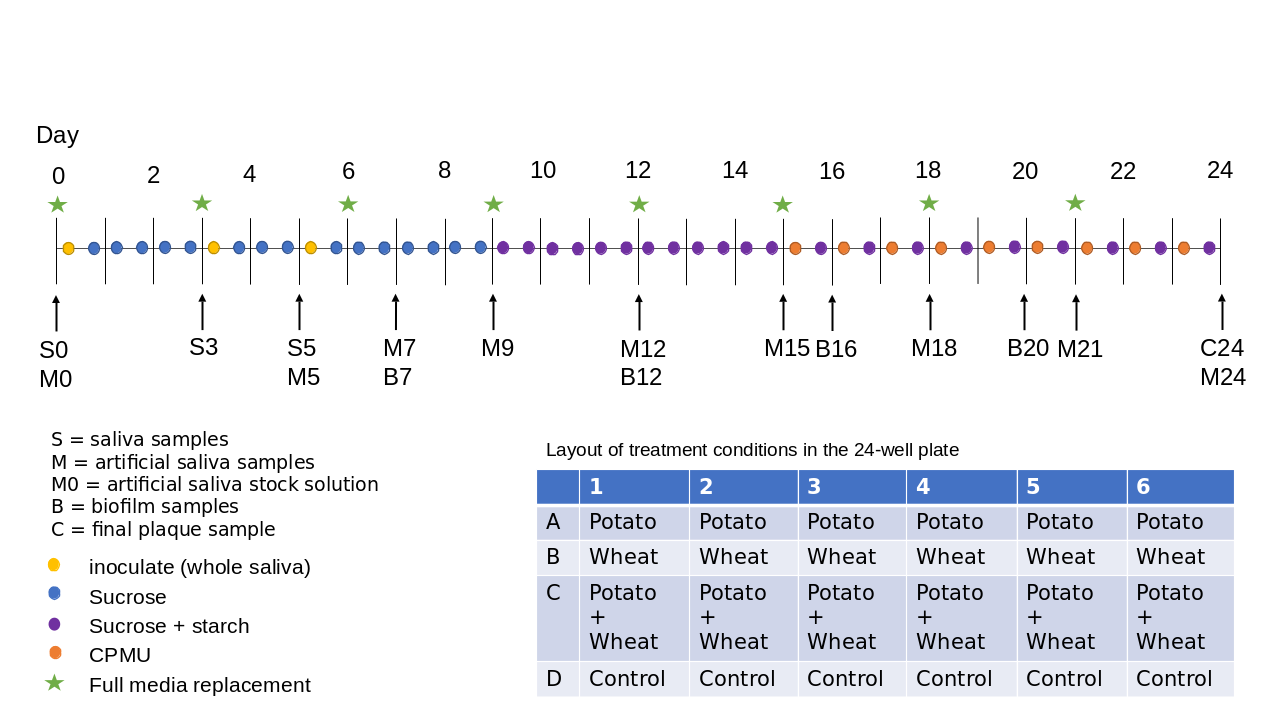
\includegraphics{figures/Exp_protocol.png}

}

\caption{\label{fig-met-protocol}Overview of the protocol for biofilm
growth. The samples for metagenomic analysis were grown in a separate
experimental plate than the FTIR samples under the same experimental
conditions. Biofilm (B) and calculus (C) samples were used for FTIR
spectroscopy, and saliva (S), artificial saliva (M), and calculus
samples were used for metagenomic analysis.}

\end{figure}%

To determine the composition of microbial communities, we sampled the
medium from the biofilm wells over the course of the experiment. We
sequenced the DNA to identify species that are present in the model, and
assess whether these mimic natural oral communities. During a separate
experimental run, under the same conditions, we directly sampled the
biofilms on multiple days and determined the mineral composition using
FTIR, and compared the spectra to those of natural dental calculus, both
modern and archaeological. Samples were taken from both controls and
starch treatments, but differences between these samples were not
explored in this study.

\subsection{Biofilm growth}\label{biofilm-growth}

We employ a multispecies oral biofilm model following a modified
protocol from Sissons and colleagues
(\citeproc{ref-sissonsMultistationPlaque1991}{1991}) and Shellis
(\citeproc{ref-shellisSyntheticSaliva1978}{1978}). The setup comprises a
polypropylene 24 deepwell PCR plate (KingFisher 97003510) with a lid
containing 24 pegs (substrata), which are autoclaved at
120\(^{\circ}\)C, 1 bar overpressure, for 20 mins.

The artificial saliva (hereafter referred to as medium) is a modified
version of the basal medium mucin (BMM) described by Sissons and
colleagues (\citeproc{ref-sissonsMultistationPlaque1991}{1991}). It is a
complex medium containing 2.5 g/l partially purified mucin from porcine
stomach (Type III, Sigma M1778), 5 g/l trypticase peptone (Roth 2363.1),
10 g/l proteose peptone (Oxoid LP0085), 5 g/l yeast extract (BD 211921),
2.5 g/l KCl, 0.35 g/l NaCl, 1.8 mmol/l CaCl\textsubscript{2}, 5.2 mmol/l
Na\textsubscript{2}HPO\textsubscript{4}
(\citeproc{ref-sissonsMultistationPlaque1991}{Sissons et al., 1991}),
6.4 mmol/l NaHCO\textsubscript{3}
(\citeproc{ref-shellisSyntheticSaliva1978}{Shellis, 1978}), 2.5 mg/l
haemin. This is subsequently adjusted to pH 7 with NaOH pellets and
stirring, autoclaved (15 min, 120\(^{\circ}\)C, 1 bar overpressure), and
supplemented with 5.8 (mu)mol/l menadione, 5 mmol/l urea, and 1 mmol/l
arginine (\citeproc{ref-sissonsMultistationPlaque1991}{Sissons et al.,
1991}).

Fresh whole saliva (WS) for inoculation was provided by a 31-year-old
male donor with no history of caries, who abstained from oral hygiene
for 24 hours, and no food was consumed two hours prior to donation. No
antibiotics were taken up to six months prior to donation. Saliva was
stimulated by chewing on parafilm, then filtered through a
bleach-sterilised nylon cloth to remove particulates. Substrata were
inoculated with 1 ml/well of a two-fold dilution of WS in sterilised
20\% glycerine for four hours at 36\(^{\circ}\)C, to allow attachment of
the salivary pellicle and plaque-forming bacteria. After initial
inoculation, the substrata were transferred to a new plate containing 1
ml/well medium and incubated at 36\(^{\circ}\)C, with gentle motion at
30 rpm. The inoculation process was repeated on days 3 and 5 by
transferring the samples to a new plate with inoculate. Medium was
partially refreshed once per day, by topping up the wells to the
original volume with more medium, and fully refreshed every three days,
throughout the experiment, by transferring the substrata to a new plate
containing medium. To feed the bacteria, the substrata were transferred
to a new plate, containing 5\% (w/v) sucrose, for six minutes twice
daily, except on inoculation days (days 0, 3, and 5), where the samples
only received one sucrose treatment after inoculation.

On day 9, starch treatments were introduced, replacing sucrose
treatments (except for control sample). As with the sucrose treatments,
starch treatments occurred twice per day for six minutes, and involved
transferring the substrata to a new plate containing a 0.25\% (w/v)
starch from potato (Roth 9441.1) solution, a 0.25\% (w/v) starch from
wheat (Sigma S5127) solution, and a 0.5\% (w/v) mixture of equal
concentrations (w/v) wheat and potato. All starch solutions were created
in a 5\% (w/v) sucrose solution. Before transferring biofilm samples to
the starch treatments, the starch plates were agitated to keep the
starches in suspension in the solutions, and during treatments, the rpm
was increased to 60. The purpose of starch treatments was to explore the
incorporation of starch granules into the model calculus. Starch
treatments were initiated on day 9 (Figure~\ref{fig-met-protocol}) to
avoid starch granule counts being affected by \(\alpha\)-amylase
hydrolysis from the inoculation saliva. An \(\alpha\)-amylase assay
conducted on samples from days 3, 6, 8, 9, 10, 12, and 14 also showed
that there was no host salivary \(\alpha\)-amylase activity in the
system. The results of the starch incorporation and \(\alpha\)-amylase
activity assay have been reported in a separate article
(\citeproc{ref-bartholdyInvestigatingBiases2022}{Bartholdy \& Henry,
2022}).

After 15 days, mineralisation was encouraged with a calcium phosphate
monofluorophosphate urea (CPMU) solution containing 20 mmol/l
CaCl\textsubscript{2}, 12 mmol/l
NaH\textsubscript{2}PO\textsubscript{4}, 5 mmol/l
Na\textsubscript{2}PO\textsubscript{3}F, 500 mmol/l urea
(\citeproc{ref-pearceConcomitantDeposition1987}{Pearce \& Sissons,
1987}; \citeproc{ref-sissonsMultistationPlaque1991}{Sissons et al.,
1991}), and 0.04 g/l MgCl. The substrata were submerged in 1 ml/well
CPMU five times daily, every two hours, for six minutes, at 30 rpm.
During the mineralisation period, starch treatments were reduced to once
per day, two hours after the last CPMU treatment. This cycle was
repeated for 10 days until the end of the experiment on day 24
(Figure~\ref{fig-met-protocol}). More detailed protocols are available
at \url{https://dx.doi.org/10.17504/protocols.io.dm6gpj9rdgzp/v1}.

All laboratory work was conducted in sterile conditions under a laminar
flow hood to prevent starch and bacterial contamination. Starch-free
control samples that were only fed sucrose were included to detect
starch contamination.

\subsection{Metagenomics}\label{metagenomics}

\begin{longtable}[]{@{}lrr@{}}

\caption{\label{tbl-dna-samples}Number of samples taken during the
experiment, separated by sampling day and sample type.}

\tabularnewline

\toprule\noalign{}
Sample type & Sampling day & n \\
\midrule\noalign{}
\endhead
\bottomrule\noalign{}
\endlastfoot
saliva & 0 & 1 \\
saliva & 3 & 1 \\
saliva & 5 & 1 \\
medium & 5 & 2 \\
medium & 7 & 2 \\
medium & 9 & 2 \\
medium & 12 & 2 \\
medium & 15 & 2 \\
medium & 18 & 2 \\
medium & 21 & 2 \\
medium & 24 & 2 \\
model\_calculus & 24 & 16 \\

\end{longtable}

A total of 35 samples were taken during the experiment from the donated
saliva, artificial saliva, and from the biofilm end-product on day 24
(Table~\ref{tbl-dna-samples}). DNA extraction was performed at the Max
Planck Institute for the Science of Human History (Jena, Germany), using
the DNeasy PowerSoil Kit from QIAGEN. C2 inhibitor removal step skipped,
going directly to C3 step.

The DNA was sheared to 500bp through sonication with a Covaris M220
Focused-ultrasonicator. Double-stranded libraries were prepared
(\citeproc{ref-aronHalfUDG2020}{Aron et al., 2020}) and dual indexed
(\citeproc{ref-stahlDoublestrandedIndexing2019}{Stahl et al., 2020}),
with the indexing protocol being adapted for longer DNA fragments.
Briefly, the modifications consisted of adding 3 μl of DMSO to the
indexing reaction, and extending the amplification cycles to
95\(^{\circ}\)C for 60 s, 58\(^{\circ}\)C for 60 s, and 72\(^{\circ}\)C
for 90 s. The libraries were paired-end sequenced on a NextSeq 500 to
150bp, and demultiplexed by an in-house script.

\subsubsection{Preprocessing}\label{preprocessing}

The raw DNA reads were preprocessed using the nf-core/eager, v2.4.4
pipeline (\citeproc{ref-yatesEAGER2020}{Fellows Yates et al., 2020}).
The pipeline included adapter removal and read merging using
AdapterRemoval, v2.3.2 (\citeproc{ref-AdapterRemovalv2}{Schubert et al.,
2016}). Merged reads were mapped to the human reference genome (GRCh38)
using BWA, v0.7.17-r1188 (\citeproc{ref-BWA}{Li \& Durbin, 2009}) (-n
0.01; -l 32), and unmapped reads were extracted using Samtools, v1.12.
The final step of the pipeline, metagenomic classification, was
conducted in kraken, v2.1.2 (\citeproc{ref-kraken2}{Wood et al., 2019})
using the Standard 60GB database
(\url{https://genome-idx.s3.amazonaws.com/kraken/k2_standard_20220926.tar.gz}).

Environmental reference samples were downloaded directly from ENA and
from NCBI using the SRA Toolkit. Oral reference samples were downloaded
from the Human Metagenome Project (HMP), and modern calculus samples
from Velsko et al. (\citeproc{ref-velskoDentalCalculus2017}{2017}). From
the HMP data, only paired reads were processed, singletons were removed.
\emph{In vitro} biofilm model samples from Edlund et al.
(\citeproc{ref-edlundUncoveringComplex2018}{2018}) were used as a
reference. Links to the specific sequences are included in the metadata.
Human-filtered reads produced in this study were uploaded to ENA under
accession number PRJEB61886.

\subsubsection{Authentication}\label{authentication}

Species with lower than 0.001\% relative abundance across all samples
were removed from the species table. SourceTracker2
(\citeproc{ref-knightsSourceTracker2011}{Knights et al., 2011}) was used
to estimate source composition of the abundance-filtered oral biofilm
model samples using a Bayesian framework, and samples falling below 70\%
oral source were removed from downstream analyses. Well-preserved
abundance-filtered samples were compared to oral and environmental
controls to detect potential external contamination. The R package
decontam v1.22.0 (\citeproc{ref-Rdecontam}{Davis et al., 2018}) was used
to identify potential contaminants in the abundance-filtered table using
DNA concentrations with a probability threshold of 0.95 and negative
controls with a probability threshold of 0.05. Putative contaminant
species were filtered out of the OTU tables for all downstream analyses.

\subsubsection{Community composition}\label{community-composition}

Relative abundances of communities were calculated at the species- and
genus-level, as recommended for compositional data
(\citeproc{ref-gloorMicrobiomeDatasets2017}{Gloor et al., 2017}).
Shannon index and Pileou's evenness index were calculated on
species-level OTU tables of all model and oral reference samples using
the vegan v2.6.4 R package (\citeproc{ref-Rvegan}{Oksanen et al.,
2022}). Shannon index was calculated for all experimental samples to see
if there is an overall loss or gain in diversity and richness across the
experiment. Sparse principal component analysis (sPCA) was performed on
model biofilm samples to assess differences in microbial composition
between samples within the experiment, and a separate sPCA analysis was
performed on model calculus and oral reference samples. The sPCA
analysis was conducted using the mixOmics v 6.26.0 R package
(\citeproc{ref-RmixOmics}{Rohart et al., 2017}).

The core microbiome was calculated by taking the mean genus-level
relative abundance within each sample type for model calculus, modern
reference calculus, sub- and supragingival plaque. Genera present at
lower than 5\% relative abundance were grouped into the category
`other'. Information on the oxygen tolerance of bacterial species was
downloaded from BacDive (\citeproc{ref-reimerBacDive2022}{Reimer et al.,
2022}) and all variations of the major categories anaerobe, facultative
anaerobe, and aerobe were combined into the appropriate major category.
At the time of writing, 55.7\% species were missing aerotolerance
values. This was mitigated by aggregating genus-level tolerances to
species with missing values, and may have some errors (although unlikely
to make any significant difference).

\subsubsection{Differential abundance}\label{differential-abundance}

Differential abundance of species was calculated using the Analysis of
Compositions of Microbiomes with Bias Correction (ANCOM-BC) method from
the ANCOMBC R package v2.4.0 (\citeproc{ref-linANCOMBC2020}{Lin \&
Peddada, 2020}), with a species-level OTU table as input. Results are
presented as the log fold change of species between paired sample types
with 95\% confidence intervals. P-values are adjusted using the false
discovery rate (FDR) method. Samples are grouped by sample type
(i.e.~saliva, plaque, modern calculus, model calculus). To supplement
the sPCA analyses, we visualised the log-fold change of the top 30
species in each of principal components 1 and 2, allowing us to see
which species are enriched in the different samples and causing
clustering in the sPCA.

\subsection{FTIR}\label{ftir}

To determine the mineral composition and level of crystallisation of the
model dental calculus samples, we used Fourier Transform Infrared (FTIR)
spectroscopy. We compared the spectra of model dental calculus with
spectra of archaeological and modern dental calculus and used a built-in
Omnic search library for mineral identification
(\citeproc{ref-mentzerDistributionAuthigenic2014}{Mentzer et al., 2014};
\citeproc{ref-weinerInfraredSpectroscopy2010}{Weiner, 2010b}). The
archaeological dental calculus was sampled from an isolated permanent
tooth from Middenbeemster, a rural, 19th century Dutch site
(\citeproc{ref-lemmersMiddenbeemster2013}{Lemmers et al., 2013}).
Samples were analysed at the Laboratory for Sedimentary Archaeology,
Haifa University. The analysis was conducted with a Thermo Scientific
Nicolet is5 spectrometer in transmission, at 4 cm\(^{-1}\) resolution,
with an average of 32 scans between 4000 and 400 cm\(^{-1}\)
wavenumbers.

\begin{longtable}[]{@{}lrrr@{}}

\caption{\label{tbl-ftir-byoc}Summary of samples used in FTIR analysis,
including type of sample, sampling day, number of samples (n), and mean
weight in mg.}

\tabularnewline

\toprule\noalign{}
Sample type & Sampling day & n & Weight (mg) \\
\midrule\noalign{}
\endhead
\bottomrule\noalign{}
\endlastfoot
biofilm & 7 & 2 & 0.79 \\
biofilm & 12 & 3 & 1.01 \\
biofilm & 16 & 7 & 2.00 \\
biofilm & 20 & 6 & 3.50 \\
model\_calculus & 24 & 8 & 3.87 \\

\end{longtable}

Analysis was conducted on 26 model calculus samples from days 7, 12, 16,
20, and 24 (Table~\ref{tbl-ftir-byoc}). Some samples from the same
sampling day had to be combined to provide enough material for analysis.
Samples analysed with FTIR were grown during a separate experimental run
from the samples sequenced for DNA, but following the same setup and
protocol (as described above). Samples were analysed following the
method presented in Asscher, Regev, et al.
(\citeproc{ref-asscherAtomicDisorder2011}{2011}) and Asscher, Weiner, et
al. (\citeproc{ref-asscherVariationsAtomic2011}{2011}). A few \(\mu\)g
of each sample were repeatedly ground together with KBr and pressed in a
7 mm die under two tons of pressure using a Specac mini-pellet press
(Specac Ltd., GS01152). Repeated measurements of the splitting factor
(SF) of the absorbance bands at 605 and 567 cm−1 wavenumbers were taken
after each grind, and a grind curve was produced following Asscher,
Regev, et al. (\citeproc{ref-asscherAtomicDisorder2011}{2011}) to try
and detect changes in the hydroxyapatite crystallinity over time.
Samples were ground and analysed up to six times (sample suffix a-f) for
the grinding curve. Grinding curves were prepared for samples from days
16, 20, and 24. No grind curves were produced for samples from days 7
and 12. These were largely composed of organics and proteins, and did
not form enough mineral (hydroxyapatite) for analysis. The splitting
factor of carbonate hydroxyapatite was calculated using a macro script,
following Weiner \& Bar-Yosef
(\citeproc{ref-weinerStatesPreservation1990}{1990}). The calculation
involves dividing the sum of the height of the absorptions at 603
cm\(^{-1}\) and 567 cm\(^{-1}\) by the height of the valley between
them. Following Asscher, Regev, et al.
(\citeproc{ref-asscherAtomicDisorder2011}{2011}) and Asscher, Weiner, et
al. (\citeproc{ref-asscherVariationsAtomic2011}{2011}), we plotted the
splitting factor against the full width at half maximum (FWHM) of the
main absorption at 1035-1043 cm\(^{-1}\) to explore crystallinity
(crystal size) and the order and disorder of hydroxyapatite. We then
compared our grinding curve slopes and FWHM to the ones produced by
Asscher, Weiner, et al.
(\citeproc{ref-asscherVariationsAtomic2011}{2011}). Asscher, Weiner, et
al. (\citeproc{ref-asscherVariationsAtomic2011}{2011}) and Asscher,
Regev, et al. (\citeproc{ref-asscherAtomicDisorder2011}{2011})
demonstrated that while the decrease in FWHM of each grinding in the
curve reflects a decrease in particle size due to grinding, the location
of the curves within a plot of the FWHM against the splitting factor
expresses the disorder effect. Thus the curves with steeper slopes,
higher splitting factor, and lower FWHM represent lower levels of
disorder in the mineral (Figure 2 in
\citeproc{ref-asscherVariationsAtomic2011}{Asscher, Weiner, et al.,
2011}).

\subsection{Statistics}\label{statistics}

Statistical analysis was conducted in R version 4.3.3 (2024-02-29)
(Angel Food Cake) (\citeproc{ref-Rbase}{R Core Team, 2020}). Data
cleaning and wrangling performed with packages from tidyverse
(\citeproc{ref-tidyverse2019}{Wickham et al., 2019}). Plots were created
using ggplot2 v3.4.4 (\citeproc{ref-ggplot2}{Wickham, 2016}).

\section{Results}\label{results}

\subsection{Metagenomic analysis}\label{metagenomic-analysis}

\subsubsection{Sample authentication}\label{sample-authentication}

To determine the extent of contamination in our samples, we performed a
source-tracking analysis using SourceTracker2
(\citeproc{ref-knightsSourceTracker2011}{Knights et al., 2011}). Results
suggest that the majority of taxa across samples have an oral microbial
signature, and therefore our samples are minimally affected by external
contamination (Figure S1). We compared SourceTracker2 results to a
database of oral taxa from the cuperdec v1.1.0 R package
(\citeproc{ref-yatesOralMicrobiome2021}{Fellows Yates et al., 2021}) to
prevent removal of samples where oral taxa were assigned to a non-oral
source (Figure S2), as some taxa with a signature from multiple sources
are often classified as ``Unknown''
(\citeproc{ref-velskoMicrobialDifferences2019}{Velsko et al., 2019}). We
included several oral sources, which may increase the risk of this
occurring. Samples containing a large proportion (\textgreater70\%) of
environmental contamination were removed. The removed samples were
predominantly medium samples from later in the experiment, and a few
model calculus samples. After contaminated samples were removed,
suspected contaminant-species were removed from the remaining samples
using the decontam R package (\citeproc{ref-Rdecontam}{Davis et al.,
2018}). After contamination removal, samples consisted of between 88 and
284 species with a mean of 182.

\subsubsection{Decrease in community diversity across
experiment}\label{decrease-in-community-diversity-across-experiment}

\begin{figure}

\centering{

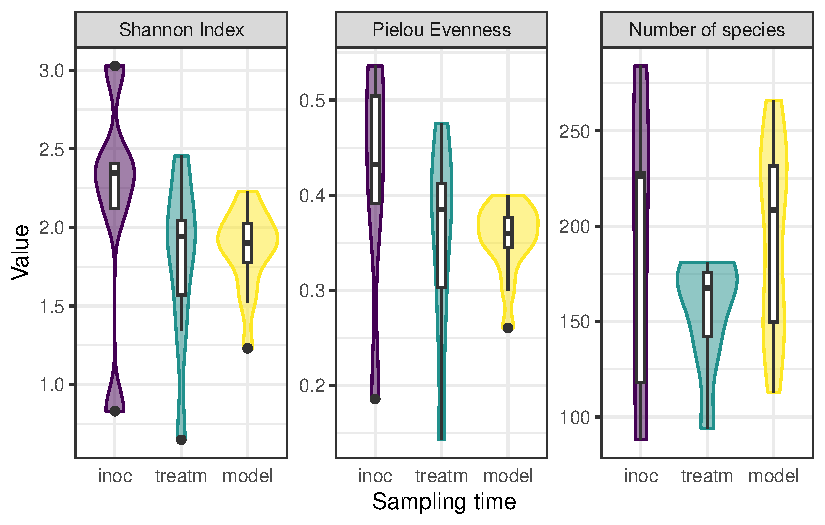
\includegraphics{figures/byoc-valid-fig-diversity-byoc-1.pdf}

}

\caption{\label{fig-diversity-byoc}Plot of Shannon Index, Pielou
Evenness Index, and number of species across experiment samples grouped
by sampling time. inoc = samples from days 0-5; treatm = samples from
days 6-23; model = model calculus samples from day 24.}

\end{figure}%

To monitor the development of microbial communities over the course of
the experiment, we used the Shannon Index to assess the species
diversity and richness at various stages of our protocol. Samples were
grouped into sampling categories due to low sample sizes on sampling
days (inoc = days 0, 3, 5; treatm = days 7, 9, 12, 15; model = day 24).
There was a slight decrease in mean Shannon Index between inoculation
and treatment samples, followed by a slight increase to model calculus
samples, as well as a decrease in variance within sample types. The
Pielou Evenness Index showed a similar pattern while the number of
species increased between the treatment period and the final model
calculus (Figure~\ref{fig-diversity-byoc}).

\subsubsection{Medium and model calculus samples are distinct from the
inoculate}\label{medium-and-model-calculus-samples-are-distinct-from-the-inoculate}

\begin{figure}

\centering{

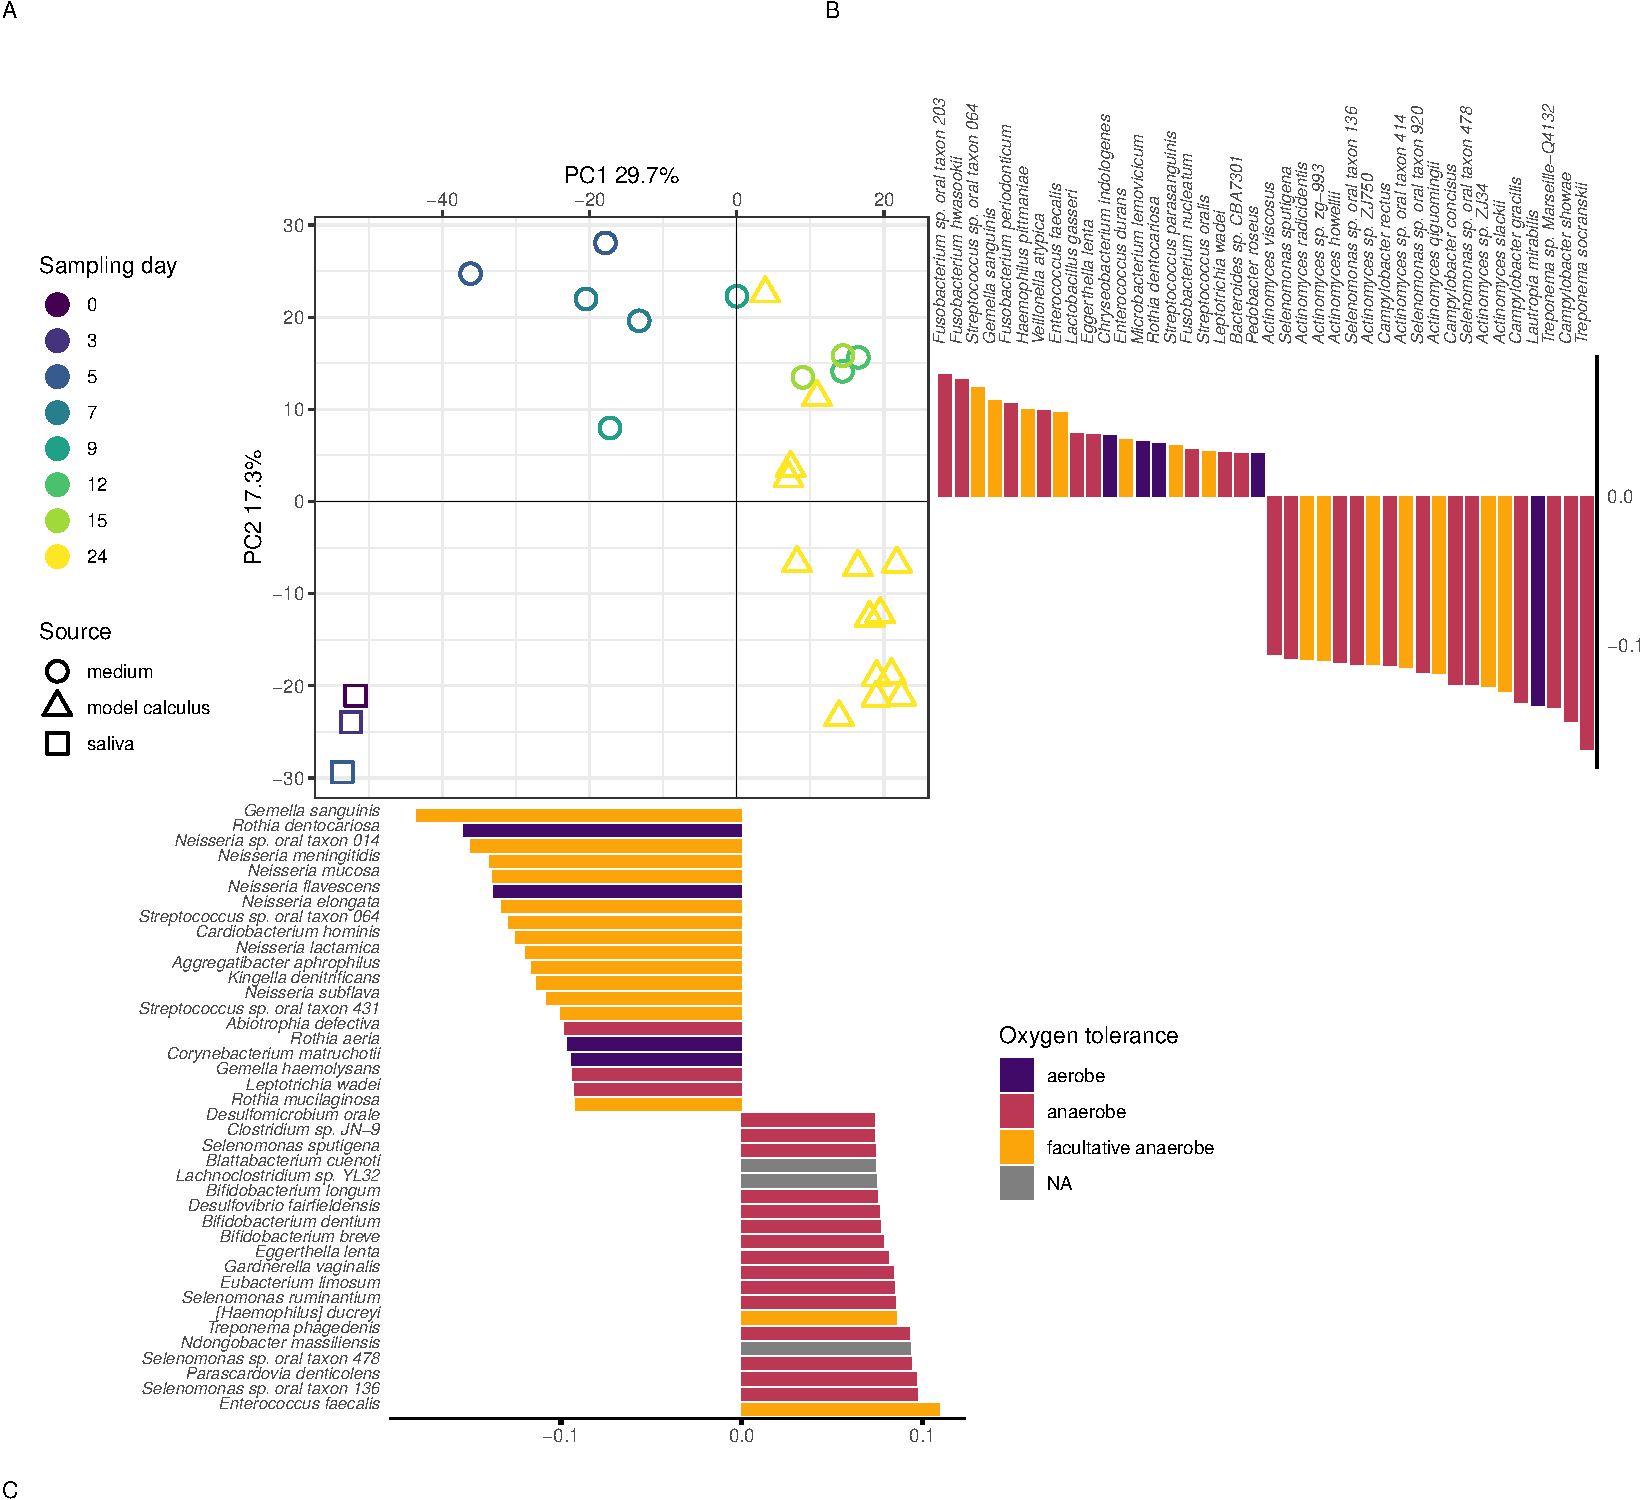
\includegraphics{figures/byoc-valid-fig-spca-byoc-1.pdf}

}

\caption{\label{fig-spca-byoc}sPCA on species-level counts and oxygen
tolerance in samples from this study only. Figure shows the main sPCA
plot (A), species loadings on PC2 (B), and species loadings on PC1 (C).}

\end{figure}%

We next examined whether there is a change in the species composition
over time in our samples by assessing the beta-diversity in a PCA. The
species profiles of the saliva inoculate used in our experiment were
distinct from both medium and model calculus samples. Most of the
separation of saliva from model calculus is on PC1 of the sPCA, where
most of the positive sample loadings are driven by anaerobic species
(model calculus), especially \emph{Selenomonas} spp, and negative
loadings are predominantly facultative anaerobes and some aerobes, such
as \emph{Rothia} and \emph{Neisseria} spp (saliva). Medium and saliva
are separated mostly on PC2, with medium samples located between saliva
and model calculus samples. Model calculus samples also cluster
separately from the medium samples on PC2, with some overlap between the
more mature medium samples and model calculus. Most of the negative
loadings separating saliva and model calculus from medium samples are
dominated by \emph{Actinomyces} spp., while positive species loadings
are more diverse, and seemingly unrelated to aerotolerance
(Figure~\ref{fig-spca-byoc}).

\begin{figure}

\centering{

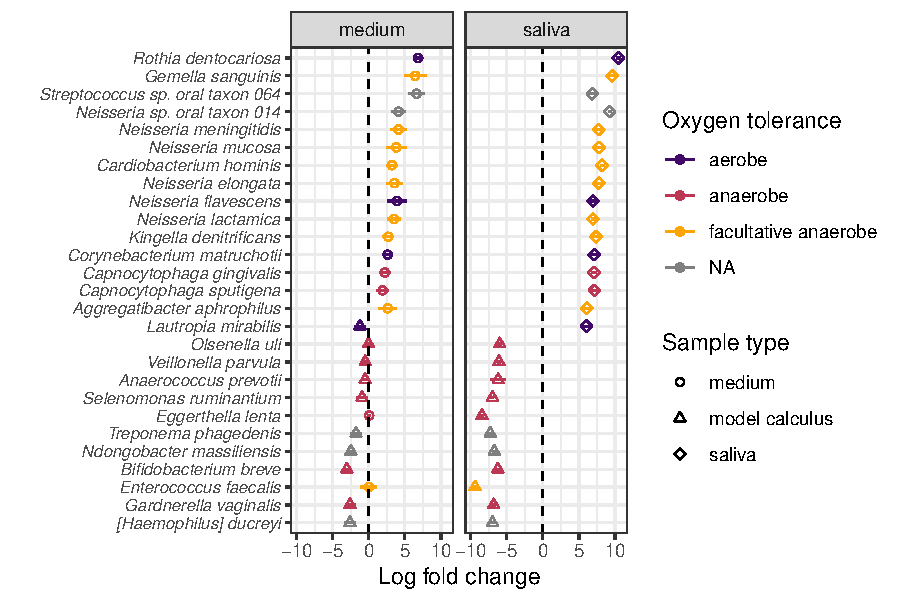
\includegraphics{figures/byoc-valid-fig-diffabund-byoc-1.pdf}

}

\caption{\label{fig-diffabund-byoc}Log-fold changes between sample
types. Circles are species enriched in the medium, triangles are
enriched in model calculus, and diamonds are enriched in saliva. Lines
are standard error. Plot shows the top 30 absolute log-fold changes
between model calculus and saliva.}

\end{figure}%

We determined whether there are species that are differentially abundant
between our sample types using the ANCOMBC R package
(\citeproc{ref-linANCOMBC2020}{Lin \& Peddada, 2020}), giving us an idea
of how the biofilm develops under our experimental conditions. Species
enriched in saliva compared to model calculus are largely aerobic or
facultatively anaerobic, while species enriched in model calculus
compared to saliva are mainly anaerobes. The differences between saliva
and calculus are more pronounced than between medium and model calculus,
which is expected (Figure~\ref{fig-diffabund-byoc}).

\subsubsection{Lower diversity in artificial samples than oral
references}\label{lower-diversity-in-artificial-samples-than-oral-references}

\begin{figure}

\centering{

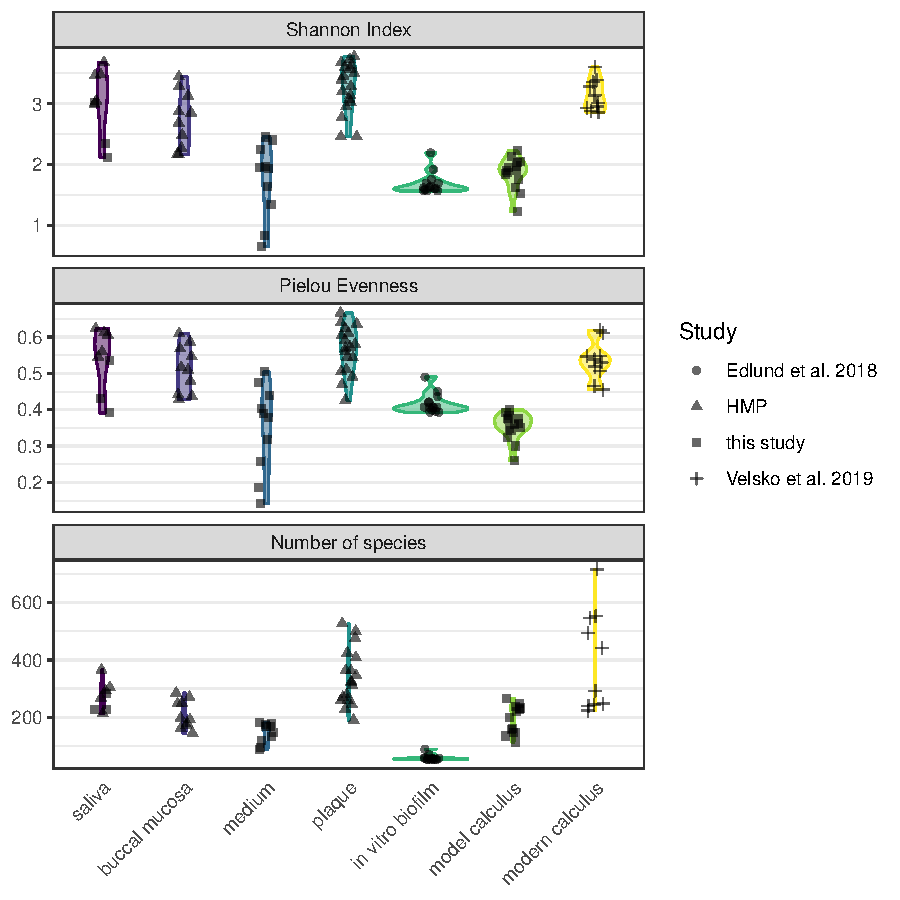
\includegraphics{figures/byoc-valid-fig-shannon-compar-1.pdf}

}

\caption{\label{fig-shannon-compar}Shannon Index for model calculus and
medium samples, as well as oral reference samples and comparative
\emph{in vitro} study.}

\end{figure}%

We used the Shannon Index to compare alpha-diversity in our model to
oral reference samples. The mean Shannon Index of model
samples---medium, model calculus, reference \emph{in vitro} biofilm were
consistently lower than the means of oral reference samples---mucosa,
modern reference dental calculus, saliva, and subgingival and
subgingival plaque. The Pielou species evenness index has a similar
distribution, although the comparative biofilm samples have a higher
mean than biofilm samples from this study. Saliva inoculate samples from
this study have a lower mean Shannon index than reference samples, which
may have contributed to the lower alpha-diversity in model samples
compared to reference samples. The number of species follows the same
trend.

\subsubsection{Model calculus is distinct from dental calculus and other
oral
samples}\label{model-calculus-is-distinct-from-dental-calculus-and-other-oral-samples}

\begin{figure}

\centering{

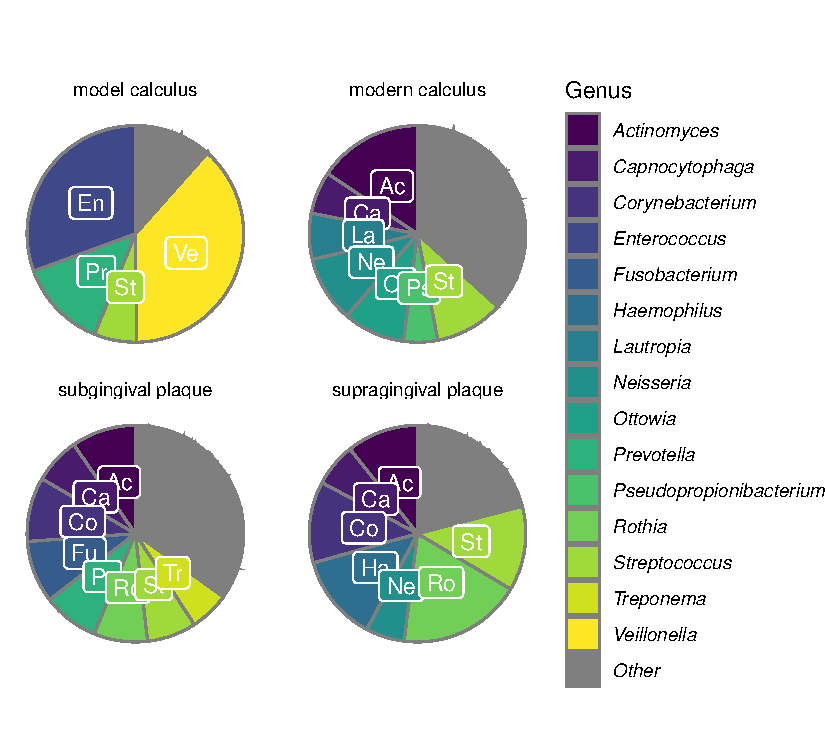
\includegraphics{figures/byoc-valid-fig-core-genera-1.pdf}

}

\caption{\label{fig-core-genera}Core genera within the different types
of samples represented as mean relative abundances at the genus level.
Other = other genera present in lower than 5\% relative abundance.}

\end{figure}%

We calculated the mean relative abundances of the genera in each sample
to compare the core genera of model calculus with oral reference
samples. The most common genera (\textgreater5\% relative abundance) are
shown in Figure~\ref{fig-core-genera}. The main overlap between the
model calculus and oral reference samples is the high relative abundance
of \emph{Streptococcus}. Model calculus consists mostly of
\emph{Enterococcus} and \emph{Veillonella} spp., despite both having low
abundance in donor saliva. \emph{Enterococcus} are also known
environmental contaminants, and we cannot exclude environmental
contamination as a possible source for these species in our model. Oral
reference samples have a more balanced composition, as they are also
represented by fastidious early-coloniser species like
\emph{Capnocytophaga} and \emph{Neisseria} spp., which require an
environment with at least 5\% carbon dioxide to thrive
(\citeproc{ref-tonjumNeisseria2017}{Tønjum \& van Putten, 2017}).

\begin{figure}

\centering{

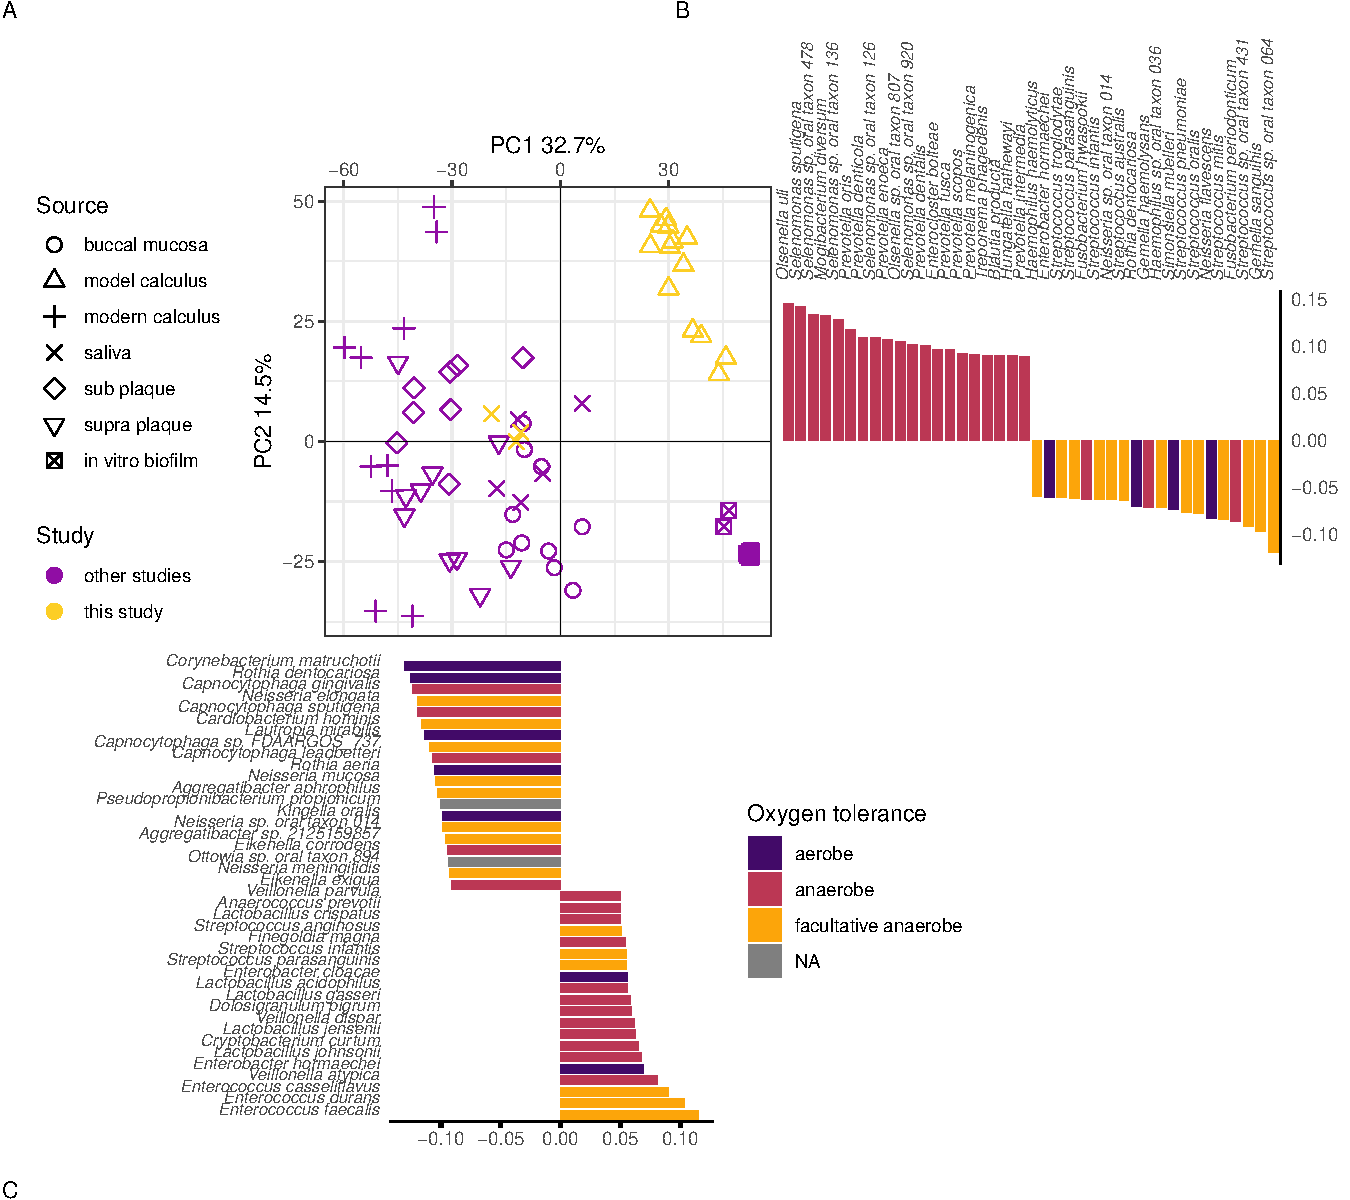
\includegraphics{figures/byoc-valid-fig-spca-compar-1.pdf}

}

\caption{\label{fig-spca-compar}sPCA on species-level counts from model
calculus and reference samples. Figure shows (A) the main sPCA plot, (B)
the species loadings from PC2, and (C) species loadings on PC1.}

\end{figure}%

To directly compare the beta-diversity of our model calculus with oral
reference samples, including modern dental calculus, we used an sPCA
including only our model calculus and reference samples. Model calculus
samples are distinct from both the oral reference samples and the
biofilm model reference samples. They are separated from oral reference
samples mainly on PC1, and from biofilm model reference samples (and, to
some extent, oral samples) on PC2. The highest negative contributions
are a mix of all types of aerotolerance, while the positive
contributions are mostly (facultative) anaerobes, with
\emph{Enterococcus} spp. as the top three positive contributors to PC1.
Top negative contributors are \emph{Capnocytophaga} spp as well as the
aerobes \emph{Corynebacterium matruchotii} and \emph{Rothia
dentocariosa}. The top positive contributors to PC2 are all anaerobes,
mainly from the genus \emph{Selenomonas}. Top negative contributors to
PC2 are a mix of aerotolerances, with many \emph{Streptococcus} spp
(Figure~\ref{fig-spca-compar}).

\begin{figure}

\centering{

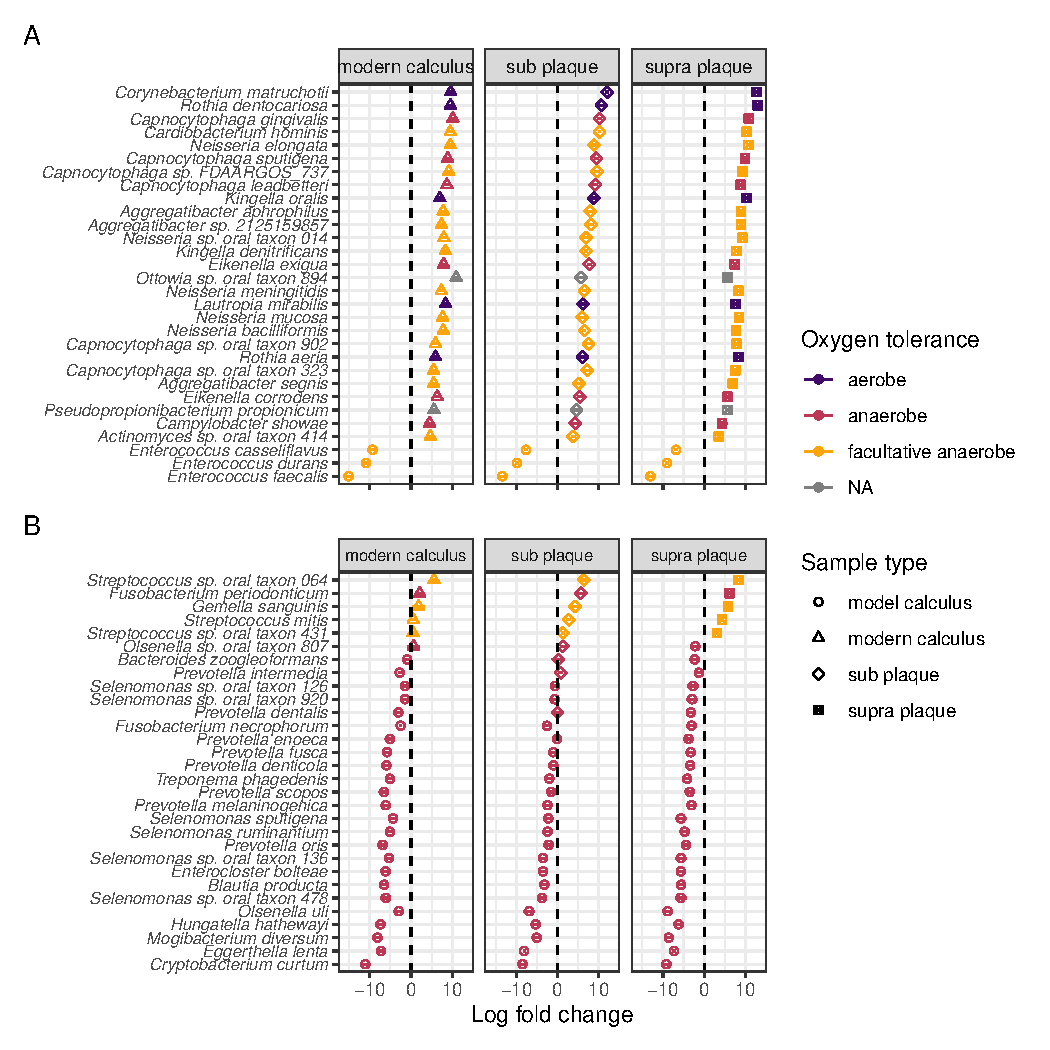
\includegraphics{figures/byoc-valid-fig-diffabund-comp-1.pdf}

}

\caption{\label{fig-diffabund-comp}Log-fold changes between sample
types. Circles are species enriched in the model calculus, triangles in
modern calculus, diamonds are enriched in subgingival plaque, and
squares in supragingival plaque. Plot shows the top 30 loadings
(absolute value) in PC1 (A) and PC2 (B) between model calculus and other
sample types, ordered by decreasing log-fold change. Bars represent
standard error.}

\end{figure}%

To investigate which species are enriched in different sample types, and
compare the final product of our model with naturally occurring plaque
and calculus samples, we performed differential abundance analysis on
our model calculus samples, modern dental calculus, and sub- and
supragingival plaque. Based on the differential abundance analysis the
main differences between model calculus and oral reference samples, when
looking at the top 30 contributors to PC1, are that the oral reference
samples are enriched with species with a diverse oxygen tolerance from a
wide range of genera, while the model calculus is enriched with
\emph{Enterococcus} spp. The largest differences occur in
\emph{Corynebacterium matruchotii}, \emph{Rothia dentocariosa}, and
\emph{Capnocytophaga gingivalis} (Figure~\ref{fig-diffabund-comp}A).
This is echoed when looking at the top 30 contributors to PC2, where
most of the species are enriched in model calculus, all of which are
anaerobes, and the largest differences occurring in
\emph{Cryptobacterium curtum}, \emph{Eggerthella lenta}, and
\emph{Mogibacterium diversum} (Figure~\ref{fig-diffabund-comp}B).

\subsection{Samples show an increased mineralisation over the course of
the
experiment}\label{samples-show-an-increased-mineralisation-over-the-course-of-the-experiment}

To determine whether the model dental calculus is comparable to natural
dental calculus, both modern and archaeological dental calculus were
analysed with FTIR spectroscopy to ascertain their composition.

It is evident that between days 7 and 24 there is a decrease of the
protein components and increase of the inorganic mineral carbonate
hydroxyapatite. The model calculus samples from the end of the
experiment are similar to both the modern and archaeological reference
samples. The main difference is a lower organic component in reference
samples seen as a reduced amide I peak at around 1637 compared to the
carbonate peak at around 1420, and an absence of amide II and III.
Further, there is a reduction in CH3 bands at 3000-2900 cm\(^{-1}\)
(Figure~\ref{fig-ftir-spectra}A-D).

Sample spectra from days 7 and 12 are characterised by a high content of
proteins as evident by the strong amide I absorbance band at 1650, a
less pronounced amide II band at 1545 cm\(^{-1}\), and the small amide
III band at 1237 cm\(^{-1}\). Related to the organic component of the
samples are also the three marked CH\textsubscript{3} and
CH\textsubscript{2} stretching vibrations at 2960, 2920, and 2850
cm\(^{-1}\) wavenumbers. The presence of mineral component is evident
from the presence of C--O\(^{2-}_3\) absorbance bands at 1450 and 1400
cm\(^{-1}\) wavenumbers typical of carbonates, and P--O\(^{3-}_4\)
absorbance band at 1080 and 1056 cm\(^{-1}\) which are related to
phosphate minerals. There is a large variation between the spectra,
possibly indicating different formation rates of the different
components in the samples (Figure~\ref{fig-ftir-spectra}A and B).

In spectra from days 16 to 24, the ratio of amides to
PO\textsubscript{4} has shifted, with the main peak shifting to the
PO\textsubscript{4} v\textsubscript{3} absorbance band at 1039--1040
cm\(^{-1}\), indicating that the main component of the samples is
carbonate hydroxyapatite. A well-defined PO\textsubscript{4} doublet at
600 and 560 is present. Small CO\(_3^{2-}\) asymmetric stretching at
1450 cm\(^{-1}\) and 1415 cm\(^{-1}\), and stretching vibrations at
875-870 cm\(^{-1}\) indicate that the carbonate minerals component is
also becoming more crystallised. There is a decreased variability
between the spectra, with most spectra exhibiting a higher
phosphate-to-protein/lipid ratio (Figure~\ref{fig-ftir-spectra}C and D).

\subsection{Model calculus has a similar mineral composition to natural
calculus}\label{model-calculus-has-a-similar-mineral-composition-to-natural-calculus}

Archaeological and modern reference spectra are largely
indistinguishable and consist of a broad O--H absorbance band (3400
cm\(^{-1}\)) related to amid a and hydroxyl group, weak CH3 bands
(3000--2900 cm\(^{-1}\)), amide I band (1650 cm\(^{-1}\)) which is
related to the protein content, carbonate (1420, 1458-1450, 875-870
cm\(^{-1}\)), and phosphates (1036-1040, 602-4, 563-566 cm\(^{-1}\))
(Figure~\ref{fig-ftir-spectra}E) which, together with the hydroxyl and
the carbonate, can be identified as derived from carbonate
hydroxyapatite, the main mineral found in mature dental calculus
(\citeproc{ref-hayashizakiSiteSpecific2008}{Hayashizaki et al., 2008};
\citeproc{ref-jinSupragingivalCalculus2002}{Jin \& Yip, 2002}).

\begin{figure}

\centering{

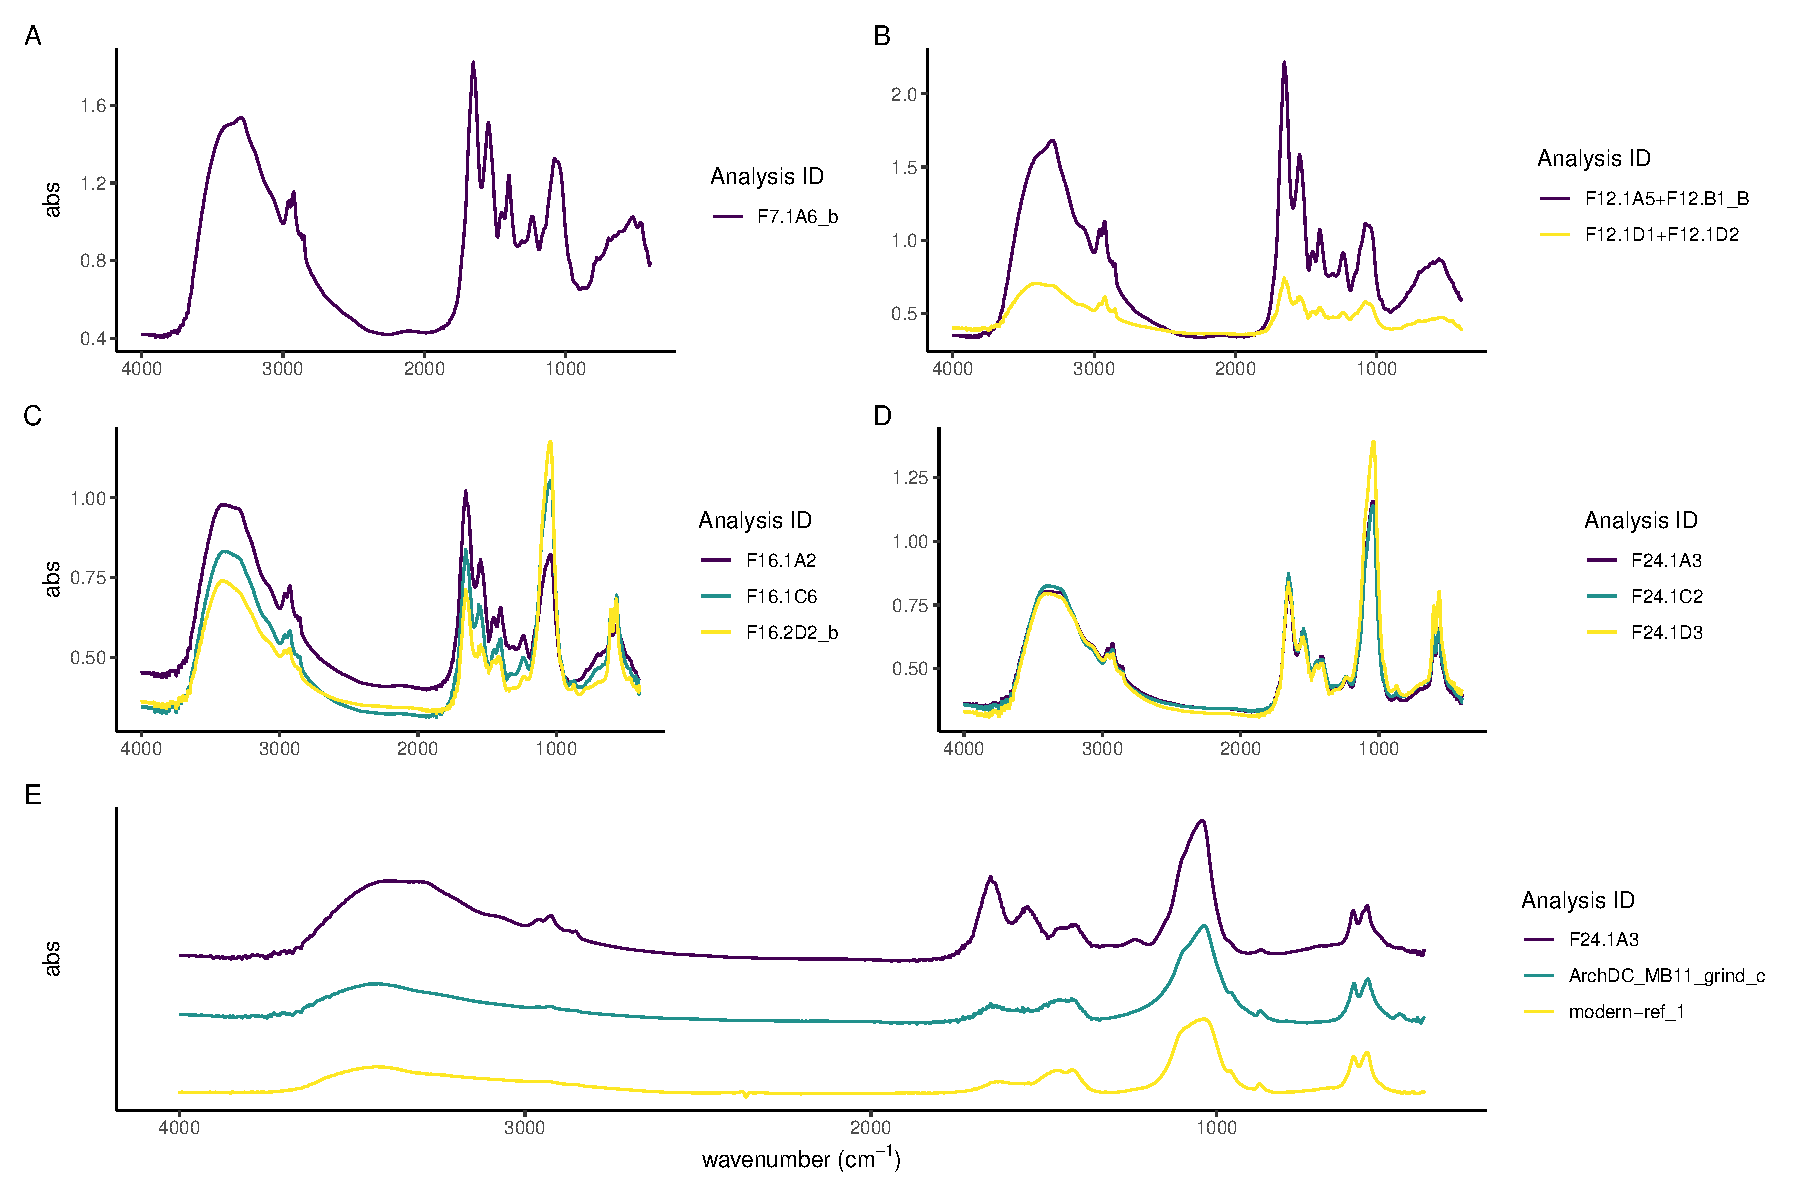
\includegraphics{figures/byoc-valid-fig-ftir-spectra-1.pdf}

}

\caption{\label{fig-ftir-spectra}Select spectra from all experiment
sampling days; (A) day 7, (B) day 12, (C) day 16, and (D) day 24.
Absorbance bands in stretching mode around 3400 cm−1 typical of the
hydroxyl group. Analysis ID for model samples is constructed as: F{[}day
sampled{]}.{[}well sampled{]}\_{[}grind sample{]}.}

\end{figure}%

\subsection{Samples show similar crystallinity and order to reference
calculus}\label{samples-show-similar-crystallinity-and-order-to-reference-calculus}

We determined the level of crystallinity and order of the carbonate
hydroxyapatite in our samples as an indication for its maturity by using
the grinding curves method presented by Asscher, Regev, et al.
(\citeproc{ref-asscherAtomicDisorder2011}{2011}) and Asscher, Weiner, et
al. (\citeproc{ref-asscherVariationsAtomic2011}{2011}).\\
Samples were compared to published trendlines for archaeological and
modern enamel (\citeproc{ref-asscherAtomicDisorder2011}{Asscher, Regev,
et al., 2011}). We see no appreciable differences between days 16, 20,
and 24. The archaeological dental calculus shows a slightly increased
slope compared to model calculus from the three sampling days used in
the grind curve (Figure~\ref{fig-grind-curve}), possibly indicating
larger crystal size due to more complete crystalisation. The steeper
slope of enamel samples is consistent with a more ordered structure in
enamel compared to dental calculus.

\begin{figure}

\centering{

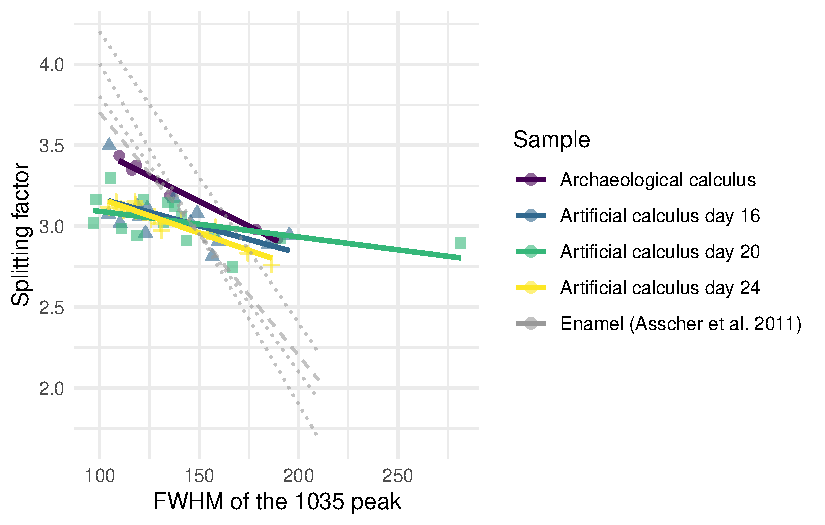
\includegraphics{figures/byoc-valid-fig-grind-curve-1.pdf}

}

\caption{\label{fig-grind-curve}Grinding curves of our biofilm and model
calculus compared to published trendlines (dashed light grey lines) for
archaeological (dotted line) and modern (dashed line) enamel.}

\end{figure}%

\section{Discussion}\label{discussion}

In this study we present a calcifying oral biofilm model to produce
artificial dental calculus. Our proposed use of the model is to address
a variety of research questions related to dietary information extracted
from dental calculus, in both modern and archaeological samples. For
that to be feasible, the model needs to serve as a viable proxy to
dental calculus grown under natural conditions, i.e., in the human oral
cavity. It needs, as much as possible, to mimic the diversity and
complexity of the natural oral microbiome, while also offering control
over factors such as dietary input, growth conditions, and replicability
within and between experiments. Here, we assessed the viability of our
model as a proxy for dental calculus using metagenomic classification
and FTIR analysis to explore the bacterial and mineral composition, and
compare with oral reference samples.

\subsection{Microbiome}\label{microbiome}

Model calculus has lower species diversity than inocula saliva and oral
reference samples, which is a common limitation in biofilm models
(\citeproc{ref-bjarnsholtVivoBiofilm2013}{Bjarnsholt et al., 2013};
\citeproc{ref-edlundBiofilmModel2013}{Edlund et al., 2013}). The donated
saliva for the experiment had a lower diversity than the reference
saliva samples, and may have contributed to a lower diversity in
experimental samples. Consequently, there is also a lower diversity and
richness when compared to other modern oral reference samples, including
oral mucosa, saliva, plaque, and calculus. Samples of the medium from
early in the experiment have similar species profiles to the donated
saliva, but gradually diverge over the course of the experiment. This
may be caused by experimental setup not sufficiently mimicking the oral
environment, allowing species to thrive that do not normally thrive in
the natural oral environment.

Oral reference samples have a relative abundance of streptococci similar
to our model, but a more diverse representation from other genera and an
overall higher species diversity and richness than our model. Reference
samples also had a more diverse aerotolerance profile than our model,
which primarily consisted of (faculatative) anaerobes. Species within
predominantly aerobic genera, are deficient in the model, suggesting a
shift from a largely aerotolerant profile to an anaerobic profile during
the experiment. While our model is not set up as an anaerobic system,
the anaerobes seem to have outcompeted aerobes and, to some extent,
facultative anaerobes. This is likely a result of communities of
bacteria within the biofilm creating favourable microenvironments
facilitated by the protective properties of the biofilm matrix
(\citeproc{ref-edlundUncoveringComplex2018}{Edlund et al., 2018};
\citeproc{ref-flemmingBiofilmsEmergent2016}{Flemming et al., 2016}).

Overall, the majority of model calculus samples contained a distinctly
oral signature, providing a promising starting point for the use of the
model as a viable proxy to dental calculus. The main differences between
model and oral reference samples may be due to human variation, as there
can be large differences in the oral microbiome of two individuals at
the species level due to variations in age, sex, and other demographic
factors, as well as how and when saliva samples were collected
(\citeproc{ref-burchamPatternsOral2020}{Burcham et al., 2020};
\citeproc{ref-nearingAssessingVariation2020}{Nearing et al., 2020}).
Whether or not distinct microbial profiles, and the extracellular matrix
they produce, will affect the retention of dietary particles in plaque
remains to be seen, but is an important question to address in the
future.

\subsection{Mineralisation}\label{mineralisation}

FTIR analysis allowed us to address the mineralisation process of the
model, which showed an increasing mineral composition over the course of
the experiment. As the model biofilm matured, the predominantly organic
content of early samples was replaced by inorganic content in the form
of carbonated hydroxyapatite, consistent with a shift from a high
presence of bacterial cells in a matrix of extracellular polysaccharides
(\citeproc{ref-jainIsolationCharacterization2013}{Jain et al., 2013};
\citeproc{ref-sutherlandBiofilmMatrix2001}{Sutherland, 2001};
\citeproc{ref-zhangMeasurementPolysaccharides1998}{Zhang et al., 1998})
to a predominantly mineral content.

The model calculus samples resemble both the modern reference calculus
and the archaeological calculus in mineral composition and
crystallinity. The steeper slope in the grind curve plots of the
archaeological sample suggests that the crystals in archaeological
samples are larger, and hence more ordered than in model calculus. A
possible explanation is that the inorganic crystals within
archaeological calculus have had more time to grow into the space left
by degraded organic matter
(\citeproc{ref-weinerBiologicalMaterials2010}{Weiner, 2010a}); however,
we only analysed one archaeological sample and cannot definitively
address this. The short duration of model calculus growth may also have
affected the results, compared to the longer-term growth and
mineralisation of natural calculus. The constant disruptions in growth
of \emph{in vivo} dental plaque/calculus, due to oral hygiene and other
external pressures on biofilm growth, may lead to multiple stages of
calcium phosphates, whereas our model has more stable growth conditions.

One of the most well-known biomineralisers, \emph{Corynebacterium
matruchotii}
(\citeproc{ref-enneverCharacterizationBacterionema1978}{Ennever et al.,
1978}; \citeproc{ref-takazoeCalciumHydroxyapatite1970}{Takazoe et al.,
1970}), exhibited a lower abundance in our model calculus compared to
modern reference calculus. However, the mineral composition of the end
results were similar, reinforcing the idea that, under the right
circumstances, biofilms with a range of microbial profiles can
facilitate mineralisation
(\citeproc{ref-moorerCalcificationCariogenic1993}{Moorer et al., 1993}).
Bacteria and their ability to secrete an extracellular matrix are
integral in the formation of dental calculus, and inevitably serve as
part of the structure that dental calculus is built upon
(\citeproc{ref-rohanizadehUltrastructuralStudy2005}{Rohanizadeh \&
LeGeros, 2005}), while the exact species composition of the biofilm
communities may be less important.

\subsection{Replicability}\label{replicability}

Model calculus displayed similar species diversity and microbial
profiles across all samples, indicating a high level of replicability
between samples in the experimental run. It remains to be seen whether
the replicability within the experiment also scales up to
between-experiment replicability in our model, though others have
already shown that replicability in long-term models is possible when
using the same inocula
(\citeproc{ref-velskoConsistentReproducible2018}{Velsko \& Shaddox,
2018}). The variation in mineral composition in our model was initially
high, but samples from day 24 were largely similar in composition as
observed in the FTIR spectra. The use of a simple multiwell plate setup
allows us to submit many samples to the same conditions, increasing
replicability between samples (\citeproc{ref-extercateAAA2010}{Exterkate
et al., 2010}).

\subsection{Limitations}\label{limitations}

While our in vitro model calculus system provides reproducible and
consistent artificial dental calculus for archaeological research, as
demonstrated by the species composition and the mineralisation
properties, we recognise the model has several limitations. Our
single-donor approach may have affected the diversity of the model. The
donated saliva from our study had a lower mean Shannon Index than other
saliva samples. The lower diversity may be caused by only using one
donor instead of pooling saliva from multiple individuals. However,
having a single inoculum donor allows us to maintain the integrity of a
native oral microbiome which may be lost when samples are pooled
(\citeproc{ref-edlundBiofilmModel2013}{Edlund et al., 2013}). It is also
possible that the diversity was affected by the collection and storage
methods we used. This has been shown to have minimal effect on microbial
profiles at the genus level (\citeproc{ref-limSalivaMicrobiome2017}{Lim
et al., 2017}), but some effect on beta diversity calculations
(\citeproc{ref-omoriComparativeEvaluation2021}{Omori et al., 2021}).

Some samples were grown with starch-sucrose solutions as nutrients,
while controls were grown with sucrose only. Due to the financial cost,
we did not sequence enough samples of each nutrient treatment to assess
the influence of starch on the microbial community or mineral
composition. Biofilms were grown in a standard shaking bacterial growth
incubator, rather than an incubator specific to cell cultures. The lack
of complex environmental control may cause the model to deviate from its
natural growth over the 25 days that the experiment is run, due to a
lack of precise control over conditions such as pH and salivary flow
rates.

There is also the possibility that contamination was introduced into the
model during the experiment. While the CPMU solution was prepared under
sterile conditions, the solution itself was not autoclaved or
filter-sterilised. In the species composition metagenomic analysis, all
medium samples collected after the introduction of CPMU on day 14 were
removed by the authentication step because the majority of species
appeared to derive from environmental sources indicating external
contamination. Going forward we recommend filter-sterilising solutions
that are not autoclaved.

To avoid disturbing the growth and development of our biofilm, we took
samples of media from the bottom of the wells after three days without
full media replacement, careful not to disturb other plate-bound
biofilms. The samples may therefore not fully reflect the composition of
the biofilm itself. Going forward we recommend sampling from the actual
biofilm, as this is the sample type under investigation.

\subsection{Future work}\label{future-work}

Further protocol optimisation will also be necessary to address some of
the limitations of our current model, such as reducing the frequency of
medium replacement (currently every three days) to help promote the
growth of slow-growing fastidious organisms and limit generalists such
as enterococci, and supplementing it with serum to provide additional
nutrients and biofilm stability
(\citeproc{ref-ammannZurichBiofilm2012}{Ammann et al., 2012};
\citeproc{ref-tianUsingDGGE2010}{Tian et al., 2010}). More infrequent
medium replacement would facilitate slow-growing bacteria in
establishing their metabolic relationships, allowing the byproducts of
some species to become abundant enough for others that depend on these
to grow (\citeproc{ref-marshDentalPlaque2005}{Marsh, 2005}).

Our goals for additional validation measures involve functional profiles
of bacteria, to see if metabolic behaviour of bacteria is consistent
with \emph{in vivo} conditions, and whether this is affected by the
presence/absence of amylase and starch treatments. The absence of host
salivary \(\alpha\)-amylase activity in our model (as shown in Bartholdy
\& Henry (\citeproc{ref-bartholdyInvestigatingBiases2022}{2022}))
provides an opportunity to explore the effect of various amylase levels
on biofilm growth and composition, as well as the incorporation of
dietary compounds in dental calculus.

The model can also be used to explore limitations and biases of methods
used to reconstruct past dietary patterns from dental calculus. To this
end, sucrose and raw starch treatments can be replaced with other
dietary components of interest, such as cooked starches, whole plant
extracts, and various proteins.

\section{Conclusions}\label{conclusions}

The bacterial profile of our model calculus is not an exact match to the
natural modern or archaeological reference calculus, but species
richness and diversity falls within a similar range as the reference
\emph{in vitro} model, and the core genera are predominantly oral. Our
model calculus had a distinct microbial profile from modern reference
calculus, but a similar mineral composition to modern and archaeological
reference calculus, consisting of carbonate hydroxyapatite and similar
levels of crystallinity and order, with a slightly higher organic phase.

Our model has many potential benefits within archaeological research,
especially since the setup does not require highly specialised
equipment, making it accessible to many labs within the archaeological
sciences. It can be used to test many fundamental aspects of the process
of incorporation, retention, and subsequent extraction of various
dietary components from archaeological dental calculus. Using an oral
biofilm model in a controlled environment with known dietary input, we
can learn more about how different methods of food processing in the
past may affect results of dental calculus analyses, and how the methods
we use may further distort this picture. Our method can be used to test
methods (e.g.~DNA, proteomics, etc.), decontamination protocols, as well
as training on these methods and protocols without depleting limited
archaeological resources. The purpose of our model is not to replace
studies conducted on archaeological and natural dental calculus, but
rather to balance limitations of each method and serve as a
complementary approach to expand our toolkit.

\section{References cited}\label{references-cited-2}

\phantomsection\label{refs-3}
\begin{CSLReferences}{1}{0}
\bibitem[\citeproctext]{ref-adlerSequencingAncient2013}
Adler, C. J., Dobney, K., Weyrich, L. S., Kaidonis, J., Walker, A. W.,
Haak, W., Bradshaw, C. J., Townsend, G., Sołtysiak, A., Alt, K. W.,
Parkhill, J., \& Cooper, A. (2013). Sequencing ancient calcified dental
plaque shows changes in oral microbiota with dietary shifts of the
{Neolithic} and {Industrial} revolutions. \emph{Nature Genetics},
\emph{45}(4), 450--455, 455e1. \url{https://doi.org/10.1038/ng.2536}

\bibitem[\citeproctext]{ref-ammannZurichBiofilm2012}
Ammann, T. W., Gmür, R., \& Thurnheer, T. (2012). Advancement of the
10-species subgingival {Zurich} biofilm model by examining different
nutritional conditions and defining the structure of the in vitro
biofilms. \emph{BMC Microbiology}, \emph{12}, 227.
\url{https://doi.org/10.1186/1471-2180-12-227}

\bibitem[\citeproctext]{ref-aronHalfUDG2020}
Aron, F., Neumann, G., \& Brandt, G. (2020). Half-{UDG} treated
double-stranded ancient {DNA} library preparation for {Illumina}
sequencing. \emph{Protocols.io}.
\url{https://doi.org/10.17504/protocols.io.bmh6k39e}

\bibitem[\citeproctext]{ref-asscherAtomicDisorder2011}
Asscher, Y., Regev, L., Weiner, S., \& Boaretto, E. (2011). Atomic
{Disorder} in {Fossil Tooth} and {Bone Mineral}: {An FTIR Study Using}
the {Grinding Curve Method}. \emph{ArcheoSciences. Revue
d'archéométrie}, \emph{35}, 135--141.
\url{https://doi.org/10.4000/archeosciences.3062}

\bibitem[\citeproctext]{ref-asscherVariationsAtomic2011}
Asscher, Y., Weiner, S., \& Boaretto, E. (2011). Variations in {Atomic
Disorder} in {Biogenic Carbonate Hydroxyapatite Using} the {Infrared
Spectrum Grinding Curve Method}. \emph{Advanced Functional Materials},
\emph{21}(17), 3308--3313. \url{https://doi.org/10.1002/adfm.201100266}

\bibitem[\citeproctext]{ref-bartholdyMultiproxyAnalysis2023}
Bartholdy, B. P., Hasselstrøm, J. B., Sørensen, L. K., Casna, M.,
Hoogland, M., Beemster, H. G., \& Henry, A. G. (2023). \emph{Multiproxy
analysis exploring patterns of diet and disease in dental calculus and
skeletal remains from a 19th century {Dutch} population}. {Zenodo}.
\url{https://doi.org/10.5281/zenodo.7649151}

\bibitem[\citeproctext]{ref-bartholdyInvestigatingBiases2022}
Bartholdy, B. P., \& Henry, A. G. (2022). Investigating {Biases
Associated With Dietary Starch Incorporation} and {Retention With} an
{Oral Biofilm Model}. \emph{Frontiers in Earth Science}, \emph{10}.
\url{https://doi.org/10.3389/feart.2022.886512}

\bibitem[\citeproctext]{ref-bjarnsholtVivoBiofilm2013}
Bjarnsholt, T., Alhede, M., Alhede, M., Eickhardt-Sørensen, S. R.,
Moser, C., Kühl, M., Jensen, P. Ø., \& Høiby, N. (2013). The in vivo
biofilm. \emph{Trends in Microbiology}, \emph{21}(9), 466--474.
\url{https://doi.org/10.1016/j.tim.2013.06.002}

\bibitem[\citeproctext]{ref-buckleyDentalCalculus2014}
Buckley, S., Usai, D., Jakob, T., Radini, A., \& Hardy, K. (2014).
Dental {Calculus Reveals Unique Insights} into {Food Items}, {Cooking}
and {Plant Processing} in {Prehistoric Central Sudan}. \emph{PLOS ONE},
\emph{9}(7), e100808. \url{https://doi.org/10.1371/journal.pone.0100808}

\bibitem[\citeproctext]{ref-burchamPatternsOral2020}
Burcham, Z. M., Garneau, N. L., Comstock, S. S., Tucker, R. M., Knight,
R., Metcalf, J. L., Genetics of Taste Lab Citizen Scientists, Miranda,
A., Reinhart, B., Meyers, D., Woltkamp, D., Boxer, E., Hutchens, J.,
Kim, K., Archer, M., McAteer, M., Huss, P., Defonseka, R., Stahle, S.,
\ldots{} Reusser, W. (2020). Patterns of {Oral Microbiota Diversity} in
{Adults} and {Children}: {A Crowdsourced Population Study}.
\emph{Scientific Reports}, \emph{10}(1), 2133.
\url{https://doi.org/10.1038/s41598-020-59016-0}

\bibitem[\citeproctext]{ref-Rdecontam}
Davis, N. M., Proctor, D. M., Holmes, S. P., Relman, D. A., \& Callahan,
B. J. (2018). Simple statistical identification and removal of
contaminant sequences in marker-gene and metagenomics data.
\emph{Microbiome}, \emph{6}(1), 226.
\url{https://doi.org/10.1186/s40168-018-0605-2}

\bibitem[\citeproctext]{ref-edlundBiofilmModel2013}
Edlund, A., Yang, Y., Hall, A. P., Guo, L., Lux, R., He, X., Nelson, K.
E., Nealson, K. H., Yooseph, S., Shi, W., \& McLean, J. S. (2013). An in
vitrobiofilm model system maintaining a highly reproducible species and
metabolic diversity approaching that of the human oral microbiome.
\emph{Microbiome}, \emph{1}(1), 25.
\url{https://doi.org/10.1186/2049-2618-1-25}

\bibitem[\citeproctext]{ref-edlundUncoveringComplex2018}
Edlund, A., Yang, Y., Yooseph, S., He, X., Shi, W., \& McLean, J. S.
(2018). Uncovering complex microbiome activities via metatranscriptomics
during 24 hours of oral biofilm assembly and maturation.
\emph{Microbiome}, \emph{6}(1), 217.
\url{https://doi.org/10.1186/s40168-018-0591-4}

\bibitem[\citeproctext]{ref-eerkensDentalCalculus2018}
Eerkens, J. W., Tushingham, S., Brownstein, K. J., Garibay, R., Perez,
K., Murga, E., Kaijankoski, P., Rosenthal, J. S., \& Gang, D. R. (2018).
Dental calculus as a source of ancient alkaloids: {Detection} of
nicotine by {LC-MS} in calculus samples from the {Americas}.
\emph{Journal of Archaeological Science: Reports}, \emph{18}, 509--515.
\url{https://doi.org/10.1016/j.jasrep.2018.02.004}

\bibitem[\citeproctext]{ref-enneverCharacterizationBacterionema1978}
Ennever, J., Riggan, L. J., Vogel, J. J., \& Boyan-Salyers, B. (1978).
Characterization of {Bacterionema} matruchotii {Calcification
Nucleator}. \emph{Journal of Dental Research}, \emph{57}(4), 637--642.
\url{https://doi.org/10.1177/00220345780570041901}

\bibitem[\citeproctext]{ref-extercateAAA2010}
Exterkate, R. A. M., Crielaard, W., \& Ten Cate, J. M. (2010). Different
{Response} to {Amine Fluoride} by {Streptococcus} mutans and
{Polymicrobial Biofilms} in a {Novel High-Throughput Active Attachment
Model}. \emph{Caries Research}, \emph{44}(4), 372--379.
\url{https://doi.org/10.1159/000316541}

\bibitem[\citeproctext]{ref-fagernasMicrobialBiogeography2022}
Fagernäs, Z., Salazar-García, D. C., Haber Uriarte, M., Avilés
Fernández, A., Henry, A. G., Lomba Maurandi, J., Ozga, A. T., Velsko, I.
M., \& Warinner, C. (2022). Understanding the microbial biogeography of
ancient human dentitions to guide study design and interpretation.
\emph{FEMS Microbes}, \emph{3}, xtac006.
\url{https://doi.org/10.1093/femsmc/xtac006}

\bibitem[\citeproctext]{ref-yatesEAGER2020}
Fellows Yates, J. A., Lamnidis, T. C., Borry, M., Valtueña, A. A.,
Fagernäs, Z., Clayton, S., Garcia, M. U., Neukamm, J., \& Peltzer, A.
(2020). Reproducible, portable, and efficient ancient genome
reconstruction with nf-core/eager. \emph{bioRxiv}, 2020.06.11.145615.
\url{https://doi.org/10.1101/2020.06.11.145615}

\bibitem[\citeproctext]{ref-yatesOralMicrobiome2021}
Fellows Yates, J. A., Velsko, I. M., Aron, F., Posth, C., Hofman, C. A.,
Austin, R. M., Parker, C. E., Mann, A. E., Nägele, K., Arthur, K. W.,
Arthur, J. W., Bauer, C. C., Crevecoeur, I., Cupillard, C., Curtis, M.
C., Dalén, L., Bonilla, M. D.-Z., Fernández-Lomana, J. C. D., Drucker,
D. G., \ldots{} Warinner, C. (2021). The evolution and changing ecology
of the {African} hominid oral microbiome. \emph{Proceedings of the
National Academy of Sciences}, \emph{118}(20).
\url{https://doi.org/10.1073/pnas.2021655118}

\bibitem[\citeproctext]{ref-filochePlaqueMicrocosm2007}
Filoche, S. K., Soma, K. J., \& Sissons, C. H. (2007). Caries-related
plaque microcosm biofilms developed in microplates. \emph{Oral
Microbiology and Immunology}, \emph{22}(2), 73--79.
\url{https://doi.org/10.1111/j.1399-302X.2007.00323.x}

\bibitem[\citeproctext]{ref-flemmingBiofilmsEmergent2016}
Flemming, H.-C., Wingender, J., Szewzyk, U., Steinberg, P., Rice, S. A.,
\& Kjelleberg, S. (2016). Biofilms: An emergent form of bacterial life.
\emph{Nature Reviews Microbiology}, \emph{14}(9), 563--575.
\url{https://doi.org/10.1038/nrmicro.2016.94}

\bibitem[\citeproctext]{ref-gloorMicrobiomeDatasets2017}
Gloor, G. B., Macklaim, J. M., Pawlowsky-Glahn, V., \& Egozcue, J. J.
(2017). Microbiome {Datasets Are Compositional}: {And This Is Not
Optional}. \emph{Frontiers in Microbiology}, \emph{8}, 2224.
\url{https://doi.org/10.3389/fmicb.2017.02224}

\bibitem[\citeproctext]{ref-hardyStarchGranules2009}
Hardy, K., Blakeney, T., Copeland, L., Kirkham, J., Wrangham, R., \&
Collins, M. (2009). Starch granules, dental calculus and new
perspectives on ancient diet. \emph{Journal of Archaeological Science},
\emph{36}(2), 248--255. \url{https://doi.org/10.1016/j.jas.2008.09.015}

\bibitem[\citeproctext]{ref-hayashizakiSiteSpecific2008}
Hayashizaki, J., Ban, S., Nakagaki, H., Okumura, A., Yoshii, S., \&
Robinson, C. (2008). Site specific mineral composition and
microstructure of human supra-gingival dental calculus. \emph{Archives
of Oral Biology}, \emph{53}(2), 168--174.
\url{https://doi.org/10.1016/j.archoralbio.2007.09.003}

\bibitem[\citeproctext]{ref-hendyProteomicCalculus2018}
Hendy, J., Warinner, C., Bouwman, A., Collins, M. J., Fiddyment, S.,
Fischer, R., Hagan, R., Hofman, C. A., Holst, M., Chaves, E., Klaus, L.,
Larson, G., Mackie, M., McGrath, K., Mundorff, A. Z., Radini, A., Rao,
H., Trachsel, C., Velsko, I. M., \& Speller, C. F. (2018). Proteomic
evidence of dietary sources in ancient dental calculus.
\emph{Proceedings. Biological Sciences}, \emph{285}(1883), 20180977.
\url{https://doi.org/10.1098/rspb.2018.0977}

\bibitem[\citeproctext]{ref-henryCalculusSyria2008}
Henry, A. G., \& Piperno, D. R. (2008). Using plant microfossils from
dental calculus to recover human diet: A case study from {Tell}
al-{Raqā}'i, {Syria}. \emph{Journal of Archaeological Science},
\emph{35}(7), 1943--1950.
\url{https://doi.org/10.1016/j.jas.2007.12.005}

\bibitem[\citeproctext]{ref-jainIsolationCharacterization2013}
Jain, K., Parida, S., Mangwani, N., Dash, H. R., \& Das, S. (2013).
Isolation and characterization of biofilm-forming bacteria and
associated extracellular polymeric substances from oral cavity.
\emph{Annals of Microbiology}, \emph{63}(4), 1553--1562.
\url{https://doi.org/10.1007/s13213-013-0618-9}

\bibitem[\citeproctext]{ref-jiFluorideMagnesium2000}
Ji, H., Nakagaki, H., Hayashizaki, J., Tsuboi, S., Kato, K., Toyama, A.,
Arai, K., Thuy, T. T., Ha, N. T. T., Kameyama, Y., Kirkham, J., \&
Robinson, C. (2000). Fluoride and magnesium concentrations in human
dental calculus obtained from {Japanese} and {Chinese} patients.
\emph{Archives of Oral Biology}, \emph{45}(7), 611--615.
\url{https://doi.org/10.1016/S0003-9969(00)00021-2}

\bibitem[\citeproctext]{ref-jinSupragingivalCalculus2002}
Jin, Y., \& Yip, H.-K. (2002). Supragingival {Calculus}: {Formation} and
{Control}. \emph{Critical Reviews in Oral Biology \& Medicine}.
\url{https://doi.org/10.1177/154411130201300506}

\bibitem[\citeproctext]{ref-kazarinaPostmedievalMicrobial2021}
Kazarina, A., Petersone-Gordina, E., Kimsis, J., Kuzmicka, J., Zayakin,
P., Griškjans, Ž., Gerhards, G., \& Ranka, R. (2021). The {Postmedieval
Latvian Oral Microbiome} in the {Context} of {Modern Dental Calculus}
and {Modern Dental Plaque Microbial Profiles}. \emph{Genes},
\emph{12}(2), 309. \url{https://doi.org/10.3390/genes12020309}

\bibitem[\citeproctext]{ref-knightsSourceTracker2011}
Knights, D., Kuczynski, J., Charlson, E. S., Zaneveld, J., Mozer, M. C.,
Collman, R. G., Bushman, F. D., Knight, R., \& Kelley, S. T. (2011).
Bayesian community-wide culture-independent microbial source tracking.
\emph{Nature Methods}, \emph{8}(9), 761--763.
\url{https://doi.org/10.1038/nmeth.1650}

\bibitem[\citeproctext]{ref-lemmersMiddenbeemster2013}
Lemmers, S. A. M., Schats, R., Hoogland, M. L. P., \& Waters-Rist, A.
(2013). {Fysisch antropologische analyse Middenbeemster}. In \emph{{De
begravingen bij de Keyserkerk te Middenbeemster}} (pp. 35--60).

\bibitem[\citeproctext]{ref-leonardPlantMicroremains2015}
Leonard, C., Vashro, L., O'Connell, J. F., \& Henry, A. G. (2015). Plant
microremains in dental calculus as a record of plant consumption: {A}
test with {Twe} forager-horticulturalists. \emph{Journal of
Archaeological Science: Reports}, \emph{2}, 449--457.
\url{https://doi.org/10.1016/j.jasrep.2015.03.009}

\bibitem[\citeproctext]{ref-BWA}
Li, H., \& Durbin, R. (2009). Fast and accurate short read alignment
with {Burrows}\textendash{{Wheeler}} transform. \emph{Bioinformatics},
\emph{25}(14), 1754--1760.
\url{https://doi.org/10.1093/bioinformatics/btp324}

\bibitem[\citeproctext]{ref-limSalivaMicrobiome2017}
Lim, Y., Totsika, M., Morrison, M., \& Punyadeera, C. (2017). The saliva
microbiome profiles are minimally affected by collection method or {DNA}
extraction protocols. \emph{Scientific Reports}, \emph{7}(1), 8523.
\url{https://doi.org/10.1038/s41598-017-07885-3}

\bibitem[\citeproctext]{ref-linANCOMBC2020}
Lin, H., \& Peddada, S. D. (2020). Analysis of compositions of
microbiomes with bias correction. \emph{Nature Communications},
\emph{11}(1), 3514. \url{https://doi.org/10.1038/s41467-020-17041-7}

\bibitem[\citeproctext]{ref-maHumanDiet2022}
Ma, Z., Liu, S., Li, Z., Ye, M., \& Huan, X. (2022). Human {Diet
Patterns During} the {Qijia Cultural Period}: {Integrated Evidence} of
{Stable Isotopes} and {Plant Micro-remains From} the {Lajia Site},
{Northwest China}. \emph{Frontiers in Earth Science}, \emph{10}.

\bibitem[\citeproctext]{ref-marshDentalPlaque2005}
Marsh, P. D. (2005). Dental plaque: Biological significance of a biofilm
and community life-style. \emph{Journal of Clinical Periodontology},
\emph{32}(s6), 7--15.
\url{https://doi.org/10.1111/j.1600-051X.2005.00790.x}

\bibitem[\citeproctext]{ref-marshDentalPlaque2006}
Marsh, P. D. (2006). Dental plaque as a biofilm and a microbial
community \textendash{} implications for health and disease. \emph{BMC
Oral Health}, \emph{6}(S1), S14.
\url{https://doi.org/10.1186/1472-6831-6-S1-S14}

\bibitem[\citeproctext]{ref-mentzerDistributionAuthigenic2014}
Mentzer, S. M., Miller, C. E., Kloos, P., Wadley, L., \& Conard, N. J.
(2014). The distribution of authigenic minerals in the {Middle Stone
Age} deposits of {Sibudu} ({South Africa}), and implications for the
preservation of archaeological features. \emph{European Society for the
Study of Human Evolution, {4thAnnual} Meeting, Florence, Italy}.

\bibitem[\citeproctext]{ref-mickleburghNewInsights2012}
Mickleburgh, H. L., \& Pagán-Jiménez, J. R. (2012). New insights into
the consumption of maize and other food plants in the pre-{Columbian
Caribbean} from starch grains trapped in human dental calculus.
\emph{Journal of Archaeological Science}, \emph{39}(7), 2468--2478.
\url{https://doi.org/10.1016/j.jas.2012.02.020}

\bibitem[\citeproctext]{ref-middletonVitroCalculus1965}
Middleton, J. D. (1965). Human salivary proteins and artificial calculus
formation in vitro. \emph{Archives of Oral Biology}, \emph{10}(2),
227--235. \url{https://doi.org/10.1016/0003-9969(65)90024-5}

\bibitem[\citeproctext]{ref-moorerCalcificationCariogenic1993}
Moorer, W. R., Ten Cate, J. M., \& Buijs, J. F. (1993). Calcification of
a {Cariogenic Streptococcus} and of {Corynebacterium} ({Bacterionema})
matruchotii. \emph{Journal of Dental Research}, \emph{72}(6),
1021--1026. \url{https://doi.org/10.1177/00220345930720060501}

\bibitem[\citeproctext]{ref-nearingAssessingVariation2020}
Nearing, J. T., DeClercq, V., Van Limbergen, J., \& Langille, M. G. I.
(2020). Assessing the {Variation} within the {Oral Microbiome} of
{Healthy Adults}. \emph{mSphere}, \emph{5}(5), e00451--20.
\url{https://doi.org/10.1128/mSphere.00451-20}

\bibitem[\citeproctext]{ref-Rvegan}
Oksanen, J., Simpson, G. L., Blanchet, F. G., Kindt, R., Legendre, P.,
Minchin, P. R., O'Hara, R. B., Solymos, P., Stevens, M. H. H., Szoecs,
E., Wagner, H., Barbour, M., Bedward, M., Bolker, B., Borcard, D.,
Carvalho, G., Chirico, M., De Caceres, M., Durand, S., \ldots{} Weedon,
J. (2022). \emph{Vegan: {Community} ecology package} {[}Manual{]}.

\bibitem[\citeproctext]{ref-omelonReviewPhosphate2013}
Omelon, S., Ariganello, M., Bonucci, E., Grynpas, M., \& Nanci, A.
(2013). A {Review} of {Phosphate Mineral Nucleation} in {Biology} and
{Geobiology}. \emph{Calcified Tissue International}, \emph{93}(4),
382--396. \url{https://doi.org/10.1007/s00223-013-9784-9}

\bibitem[\citeproctext]{ref-omoriComparativeEvaluation2021}
Omori, M., Kato-Kogoe, N., Sakaguchi, S., Fukui, N., Yamamoto, K.,
Nakajima, Y., Inoue, K., Nakano, H., Motooka, D., Nakano, T., Nakamura,
S., \& Ueno, T. (2021). Comparative evaluation of microbial profiles of
oral samples obtained at different collection time points and using
different methods. \emph{Clinical Oral Investigations}, \emph{25}(5),
2779--2789. \url{https://doi.org/10.1007/s00784-020-03592-y}

\bibitem[\citeproctext]{ref-pearceConcomitantDeposition1987}
Pearce, E. I. F., \& Sissons, C. H. (1987). The {Concomitant Deposition}
of {Strontium} and {Fluoride} in {Dental Plaque}. \emph{Journal of
Dental Research}, \emph{66}(10), 1518--1522.
\url{https://doi.org/10.1177/00220345870660100101}

\bibitem[\citeproctext]{ref-powerChimpCalculus2015}
Power, R. C., Salazar-Garcia, D. C., Wittig, R. M., Freiberg, M., \&
Henry, A. G. (2015). Dental calculus evidence of {Tai Forest Chimpanzee}
plant consumption and life history transitions. \emph{Scientific
Reports}, \emph{5}, 15161. \url{https://doi.org/10.1038/srep15161}

\bibitem[\citeproctext]{ref-Rbase}
R Core Team. (2020). \emph{R: {A} language and environment for
statistical computing} {[}Manual{]}. {R Foundation for Statistical
Computing}.

\bibitem[\citeproctext]{ref-radiniDirtyTeeth2022}
Radini, A., \& Nikita, E. (2022). Beyond dirty teeth: {Integrating}
dental calculus studies with osteoarchaeological parameters.
\emph{Quaternary International}.
\url{https://doi.org/10.1016/j.quaint.2022.03.003}

\bibitem[\citeproctext]{ref-reimerBacDive2022}
Reimer, L. C., Sardà Carbasse, J., Koblitz, J., Ebeling, C., Podstawka,
A., \& Overmann, J. (2022). {BacDive} in 2022: The knowledge base for
standardized bacterial and archaeal data. \emph{Nucleic Acids Research},
\emph{50}(D1), D741--D746. \url{https://doi.org/10.1093/nar/gkab961}

\bibitem[\citeproctext]{ref-rohanizadehUltrastructuralStudy2005}
Rohanizadeh, R., \& LeGeros, R. Z. (2005). Ultrastructural study of
calculus\textendash enamel and calculus\textendash root interfaces.
\emph{Archives of Oral Biology}, \emph{50}(1), 89--96.
\url{https://doi.org/10.1016/j.archoralbio.2004.07.001}

\bibitem[\citeproctext]{ref-RmixOmics}
Rohart, F., Gautier, B., Singh, A., \& Le Cao, K.-A. (2017). {mixOmics}:
{An R} package for 'omics feature selection and multiple data
integration. \emph{PLoS Computational Biology}, \emph{13}(11), e1005752.

\bibitem[\citeproctext]{ref-AdapterRemovalv2}
Schubert, M., Lindgreen, S., \& Orlando, L. (2016). {AdapterRemoval} v2:
Rapid adapter trimming, identification, and read merging. \emph{BMC
Research Notes}, \emph{9}, 88.
\url{https://doi.org/10.1186/s13104-016-1900-2}

\bibitem[\citeproctext]{ref-shellisSyntheticSaliva1978}
Shellis, R. P. (1978). A synthetic saliva for cultural studies of dental
plaque. \emph{Archives of Oral Biology}, \emph{23}(6), 485--489.
\url{https://doi.org/10.1016/0003-9969(78)90081-X}

\bibitem[\citeproctext]{ref-sissonsMultistationPlaque1991}
Sissons, C. H., Cutress, T. W., Hoffman, M. P., \& Wakefield, J. S. J.
(1991). A {Multi-station Dental Plaque Microcosm} ({Artificial Mouth})
for the {Study} of {Plaque Growth}, {Metabolism}, {pH}, and
{Mineralization}: \emph{Journal of Dental Research}.
\url{https://doi.org/10.1177/00220345910700110301}

\bibitem[\citeproctext]{ref-stahlDoublestrandedIndexing2019}
Stahl, R., Warinner, C., Velsko, I., Orfanou, E., Aron, F., \& Brandt,
G. (2020). Illumina double-stranded {DNA} dual indexing for ancient
{DNA}. \emph{Protocols.io}.
\url{https://doi.org/10.17504/protocols.io.4r3l287x3l1y/v3}

\bibitem[\citeproctext]{ref-sutherlandBiofilmMatrix2001}
Sutherland, I. W. (2001). The biofilm matrix \textendash{} an
immobilized but dynamic microbial environment. \emph{Trends in
Microbiology}, \emph{9}(5), 222--227.
\url{https://doi.org/10.1016/S0966-842X(01)02012-1}

\bibitem[\citeproctext]{ref-takazoeCalciumHydroxyapatite1970}
Takazoe, I., Vogel, J., \& Ennever, J. (1970). Calcium {Hydroxyapatite
Nucleation} by {Lipid Extract} of {Bacterionema} matruchotii.
\emph{Journal of Dental Research}, \emph{49}(2), 395--398.
\url{https://doi.org/10.1177/00220345700490023301}

\bibitem[\citeproctext]{ref-tianUsingDGGE2010}
Tian, Y., He, X., Torralba, M., Yooseph, S., Nelson, K. e., Lux, R.,
McLean, J. s., Yu, G., \& Shi, W. (2010). Using {DGGE} profiling to
develop a novel culture medium suitable for oral microbial communities.
\emph{Molecular Oral Microbiology}, \emph{25}(5), 357--367.
\url{https://doi.org/10.1111/j.2041-1014.2010.00585.x}

\bibitem[\citeproctext]{ref-tonjumNeisseria2017}
Tønjum, T., \& van Putten, J. (2017). 179 - {Neisseria}. In J. Cohen, W.
G. Powderly, \& S. M. Opal (Eds.), \emph{Infectious {Diseases} ({Fourth
Edition})} (pp. 1553--1564.e1). {Elsevier}.
\url{https://doi.org/10.1016/B978-0-7020-6285-8.00179-9}

\bibitem[\citeproctext]{ref-trompEDTACalculus2017}
Tromp, M., Buckley, H., Geber, J., \& Matisoo-Smith, E. (2017). {EDTA}
decalcification of dental calculus as an alternate means of
microparticle extraction from archaeological samples. \emph{Journal of
Archaeological Science: Reports}, \emph{14}, 461--466.
\url{https://doi.org/10.1016/j.jasrep.2017.06.035}

\bibitem[\citeproctext]{ref-velskoCytokineResponse2017}
Velsko, I. M., Cruz-Almeida, Y., Huang, H., Wallet, S. M., \& Shaddox,
L. M. (2017). Cytokine response patterns to complex biofilms by
mononuclear cells discriminate patient disease status and biofilm
dysbiosis. \emph{Journal of Oral Microbiology}, \emph{9}(1), 1330645.
\url{https://doi.org/10.1080/20002297.2017.1330645}

\bibitem[\citeproctext]{ref-velskoMicrobialDifferences2019}
Velsko, I. M., Fellows Yates, J. A., Aron, F., Hagan, R. W., Frantz, L.
A. F., Loe, L., Martinez, J. B. R., Chaves, E., Gosden, C., Larson, G.,
\& Warinner, C. (2019). Microbial differences between dental plaque and
historic dental calculus are related to oral biofilm maturation stage.
\emph{Microbiome}, \emph{7}(1), 102.
\url{https://doi.org/10.1186/s40168-019-0717-3}

\bibitem[\citeproctext]{ref-velskoDentalCalculus2017}
Velsko, I. M., Overmyer, K. A., Speller, C., Klaus, L., Collins, M. J.,
Loe, L., Frantz, L. A. F., Sankaranarayanan, K., Lewis, C. M., Martinez,
J. B. R., Chaves, E., Coon, J. J., Larson, G., \& Warinner, C. (2017).
The dental calculus metabolome in modern and historic samples.
\emph{Metabolomics}, \emph{13}(11), 134.
\url{https://doi.org/10.1007/s11306-017-1270-3}

\bibitem[\citeproctext]{ref-velskoConsistentReproducible2018}
Velsko, I. M., \& Shaddox, L. M. (2018). Consistent and reproducible
long-term in vitro growth of health and disease-associated oral
subgingival biofilms. \emph{BMC Microbiology}, \emph{18}(1), 70.
\url{https://doi.org/10.1186/s12866-018-1212-x}

\bibitem[\citeproctext]{ref-warinnerPathogensHost2014}
Warinner, C., Rodrigues, J. F., Vyas, R., Trachsel, C., Shved, N.,
Grossmann, J., Radini, A., Hancock, Y., Tito, R. Y., Fiddyment, S.,
Speller, C., Hendy, J., Charlton, S., Luder, H. U., Salazar-Garcia, D.
C., Eppler, E., Seiler, R., Hansen, L. H., Castruita, J. A., \ldots{}
Cappellini, E. (2014). Pathogens and host immunity in the ancient human
oral cavity. \emph{Nature Genetics}, \emph{46}(4), 336--344.
\url{https://doi.org/10.1038/ng.2906}

\bibitem[\citeproctext]{ref-warinnerNewEra2015}
Warinner, C., Speller, C., \& Collins, M. J. (2015). A new era in
palaeomicrobiology: Prospects for ancient dental calculus as a long-term
record of the human oral microbiome. \emph{Philosophical Transactions of
the Royal Society B: Biological Sciences}, \emph{370}(1660), 20130376.
\url{https://doi.org/10.1098/rstb.2013.0376}

\bibitem[\citeproctext]{ref-weinerBiologicalMaterials2010}
Weiner, S. (2010a). Biological {Materials}: {Bones} and {Teeth}. In
\emph{Microarchaeology: {Beyond} the {Visible Archaeological Record}}
(pp. 99--134). {Cambridge University Press}.

\bibitem[\citeproctext]{ref-weinerInfraredSpectroscopy2010}
Weiner, S. (2010b). Infrared {Spectroscopy} in {Archaeology}. In
\emph{Microarchaeology: {Beyond} the {Visible Archaeological Record}}
(First, pp. 275--316). {Cambridge University Press}.
\url{https://doi.org/10.1017/CBO9780511811210}

\bibitem[\citeproctext]{ref-weinerStatesPreservation1990}
Weiner, S., \& Bar-Yosef, O. (1990). States of preservation of bones
from prehistoric sites in the {Near East}: {A} survey. \emph{Journal of
Archaeological Science}, \emph{17}(2), 187--196.
\url{https://doi.org/10.1016/0305-4403(90)90058-D}

\bibitem[\citeproctext]{ref-whiteDentalCalculus1997}
White, D. J. (1997). Dental calculus: Recent insights into occurrence,
formation, prevention, removal and oral health effects of supragingival
and subgingival deposits. \emph{European Journal of Oral Sciences},
\emph{105}(5), 508--522.
\url{https://doi.org/10.1111/j.1600-0722.1997.tb00238.x}

\bibitem[\citeproctext]{ref-ggplot2}
Wickham, H. (2016). \emph{Ggplot2: {Elegant Graphics} for {Data
Analysis}}. {Springer-Verlag}.

\bibitem[\citeproctext]{ref-tidyverse2019}
Wickham, H., Averick, M., Bryan, J., Chang, W., McGowan, L. D.,
François, R., Grolemund, G., Hayes, A., Henry, L., Hester, J., Kuhn, M.,
Pedersen, T. L., Miller, E., Bache, S. M., Müller, K., Ooms, J.,
Robinson, D., Seidel, D. P., Spinu, V., \ldots{} Yutani, H. (2019).
Welcome to the {tidyverse}. \emph{Journal of Open Source Software},
\emph{4}(43), 1686. \url{https://doi.org/10.21105/joss.01686}

\bibitem[\citeproctext]{ref-wongCalciumPhosphate2002}
Wong, L., Sissons, C. H., Pearce, E. I. F., \& Cutress, T. W. (2002).
Calcium phosphate deposition in human dental plaque microcosm biofilms
induced by a ureolytic {pH-rise} procedure. \emph{Archives of Oral
Biology}, \emph{47}(11), 779--790.
\url{https://doi.org/10.1016/S0003-9969(02)00114-0}

\bibitem[\citeproctext]{ref-kraken2}
Wood, D. E., Lu, J., \& Langmead, B. (2019). Improved metagenomic
analysis with {Kraken} 2. \emph{Genome Biology}, \emph{20}(1), 257.
\url{https://doi.org/10.1186/s13059-019-1891-0}

\bibitem[\citeproctext]{ref-zhangMeasurementPolysaccharides1998}
Zhang, X., Bishop, P. L., \& Kupferle, M. J. (1998). Measurement of
polysaccharides and proteins in biofilm extracellular polymers.
\emph{Water Science and Technology}, \emph{37}(4), 345--348.
\url{https://doi.org/10.1016/S0273-1223(98)00127-9}

\end{CSLReferences}

\bookmarksetup{startatroot}

\chapter{Article 2}\label{article-2}

Investigating Biases Associated with Dietary Starch Incorporation and
Retention with an Oral Biofilm Model

\hfill\break

\footnotesize

\textbf{Co-authors and contributions:}

\begin{itemize}
\tightlist
\item
  Amanda G. Henry, Leiden University
\end{itemize}

Conceptualization: B.P.B. and A.G.H. Data curation: B.P.B. Formal
analysis: B.P.B. Funding acquisition: A.G.H. Investigation: B.P.B.
Methodology: B.P.B. and A.G.H. Resources: A.G.H. Software: B.P.B.
Supervision: A.G.H. Visualization: B.P.B. Writing - original draft:
B.P.B. Writing - review \& editing: B.P.B. and A.G.H.

\textbf{Cite as:}

Bartholdy, B. P., \& Henry, A. G. (2022). Investigating Biases
Associated With Dietary Starch Incorporation and Retention With an Oral
Biofilm Model. Frontiers in Earth Science, 10.
https://doi.org/10.3389/feart.2022.886512

\normalsize

\newpage{}

\section{Introduction}\label{byocstarch-intro}

Dental calculus has proven to contain a wealth of dietary information in
the form of plant microfossils
(\citeproc{ref-hardyStarchGranules2009}{Hardy et al., 2009};
\citeproc{ref-henryCalculusSyria2008}{Henry \& Piperno, 2008}), proteins
(\citeproc{ref-hendyProteomicCalculus2018}{Hendy et al., 2018};
\citeproc{ref-warinnerEvidenceMilk2014}{Warinner, Hendy, et al., 2014}),
and other organic residues
(\citeproc{ref-buckleyDentalCalculus2014}{Buckley et al., 2014}). This
dietary information can be preserved within the mineralised dental
plaque over many millennia, providing a unique window into the
food-related behaviours of past populations
(\citeproc{ref-henryCalculusSyria2008}{Henry \& Piperno, 2008};
\citeproc{ref-jovanovicNeolithicCalculus2021}{Jovanović et al., 2021};
\citeproc{ref-taoWheatCalculus2020}{Tao et al., 2020}) and extinct
species (\citeproc{ref-hardyNeanderthalMedics2012}{Hardy et al., 2012};
\citeproc{ref-henryNeanderthalCalculus2014}{Henry et al., 2014}).

Until recently, only a few studies directly investigated the presence of
plant microremains in the dental calculus of archaeological remains. The
ability to extract phytoliths from the dental calculus of archaeological
fauna to investigate diet was first noted by Armitage
(\citeproc{ref-armitageExtractionIdentification1975}{1975}), and later
by Middleton and Rovner
(\citeproc{ref-middletonOpalPhytoliths1994}{1994}), and Fox and
colleagues (\citeproc{ref-foxPhytolithCalculus1996}{1996}). Starches and
phytoliths were extracted from human dental calculus by Cummings and
Magennis (\citeproc{ref-cummingsMayanCalculus1997}{1997}).\\
In more recent years, the study of dental calculus has increased
exponentially, and the wealth of information contained within the
mineralised matrix has largely been acknowledged. The use of dental
calculus spans a wide variety of archaeological research areas, such as
oral microbiome characterisation (including pathogens) through the
analysis of DNA and proteins
(\citeproc{ref-adlerSequencingAncient2013}{Adler et al., 2013};
\citeproc{ref-warinnerPathogensHost2014}{Warinner, Rodrigues, et al.,
2014}), microbotanical remains
(\citeproc{ref-hardyStarchGranules2009}{Hardy et al., 2009};
\citeproc{ref-henryCalculusSyria2008}{Henry \& Piperno, 2008};
\citeproc{ref-mickleburghNewInsights2012}{Mickleburgh \& Pagán-Jiménez,
2012}), other organic residues and proteins from dietary compounds
(\citeproc{ref-buckleyDentalCalculus2014}{Buckley et al., 2014};
\citeproc{ref-hendyProteomicCalculus2018}{Hendy et al., 2018}), and
nicotine use (\citeproc{ref-eerkensDentalCalculus2018}{Eerkens et al.,
2018}). Especially the extraction of starch granules has become a rich
source of dietary information, as starch granules have proven to
preserve well within dental calculus over a variety of geographical and
temporal ranges (\citeproc{ref-henryNeanderthalCalculus2014}{Henry et
al., 2014}; \citeproc{ref-jovanovicNeolithicCalculus2021}{Jovanović et
al., 2021}; \citeproc{ref-pipernoStarchGrains2008}{Piperno \& Dillehay,
2008}; \citeproc{ref-taoWheatCalculus2020}{Tao et al., 2020}).

Despite this, our knowledge of dental calculus and the incorporation
pathways of the various markers is limited
(\citeproc{ref-radiniFoodPathways2017}{Radini et al., 2017}), as is our
knowledge of information-loss caused by these pathways. Additionally,
the methods we use to extract and analyse dental calculus, and make
inferences on past diets represent another potential source of bias.
Studies on both archaeological and modern individuals have explored
these biases in more detail. Extraction methods were tested by Tromp and
colleagues (\citeproc{ref-trompEDTACalculus2017}{2017}), specifically
regarding decalcification using HCl or EDTA. The authors found
significantly more starches with the EDTA extraction method than the HCl
extraction method; however, as noted by the authors, comparisons
involving archaeological calculus are problematic due to variability
between and within individuals. Studies conducted on modern humans
(\citeproc{ref-leonardPlantMicroremains2015}{Leonard et al., 2015}) and
non-human primates (\citeproc{ref-powerChimpCalculus2015}{R. C. Power et
al., 2015}; \citeproc{ref-powerRepresentativenessDental2021}{Robert C.
Power et al., 2021}) have explored how well microremains (phytoliths and
starches) extracted from dental calculus represent the actual dietary
intake. These studies are justifiably limited, despite meticulous
documentation and observation, due to unknown variables and uncertainty
involved in this kind of \emph{in vivo} research. Dental calculus is a
complex oral biofilm with a multifactorial aetiology and variable
formation rates both within and between individuals
(\citeproc{ref-haffajeeBiofilmPosition2009}{Haffajee et al., 2009};
\citeproc{ref-jepsenCalculusRemoval2011}{Jepsen et al., 2011}),
contributing to the stochasticity of starch representation being
observed in numerous studies. Additionally, the concentration of oral
\(\alpha\)-amylase differs both between and within individuals
(\citeproc{ref-froehlichEffectOral1987}{Froehlich et al., 1987};
\citeproc{ref-naterHumanAmylase2005}{Nater et al., 2005}), causing
different rates of hydrolysis of the starch granules present in the oral
cavity. Add to this the effects of the many different methods of starch
processing (\citeproc{ref-hardyRecoveringInformation2018}{Hardy et al.,
2018}), as well as post-depositional processes that are still being
explored (\citeproc{ref-graneroStarchTaphonomy2020}{García-Granero,
2020}; \citeproc{ref-mercaderExaggeratedExpectations2018}{Mercader et
al., 2018}), and it becomes clear that using dental calculus to
reconstruct diet is a highly unpredictable process.

In this exploratory study, we use an oral biofilm model to investigate
the retention of starch granules within dental calculus in a controlled
laboratory setting, allowing us full control over dietary input. Our
main questions concern the representation of granules extracted from the
calculus compared to the actual intake. How much of the original diet is
incorporated into the calculus, and how much is recovered? Is there
differential loss of information from specific dietary markers that
affects the obtained dietary information, and how does this affect the
representation of diet from extracted microremains?\\
We find that, despite the absence of \(\alpha\)-amylase in the model, a
limited proportion of the starch input is actually retained in the
calculus. We also observed a shift in the size ratios of individual
starch granules that are incorporated into the calculus, and that the
number of incorporated starch granules increases as the size of the
calculus deposit increases.

\section{Materials and Methods}\label{materials-and-methods-1}

\subsection{Biofilm formation}\label{biofilm-formation}

In this study we employ a multispecies oral biofilm model following a
modified protocol from Sissons and colleagues
(\citeproc{ref-sissonsMultistationPlaque1991}{1991}) and Shellis
(\citeproc{ref-shellisSyntheticSaliva1978}{1978}). In brief, a biofilm
inoculated with whole saliva was grown on a substrate suspended in
artificial saliva, and fed with sugar (sucrose). After several days of
growth, the biofilm was exposed to starch solutions. Mineralisation of
the biofilm was aided by exposure to a calcium phosphate solution. After
25 days of growth, the mineralised biofilm was collected for further
analysis. The setup comprises a polypropylene 24 deepwell PCR plate
(KingFisher 97003510) with a lid containing 24 pegs, which is autoclaved
at 120°C, 1 bar overpressure, for 20 mins. The individual pegs were the
substrata on which the calculus grew. Using this system allowed for easy
transfer of the growing biofilm between saliva, feeding solutions, and
mineral solutions.

The artificial saliva (AS) is a modified version of the basal medium
mucin (BMM) described by Sissons and colleagues
(\citeproc{ref-sissonsMultistationPlaque1991}{1991}). It contains 2.5
g/l partially purified mucin from porcine stomach (Type III, Sigma
M1778), 5 g/l trypticase peptone (Roth 2363.1), 10 g/l proteose peptone
(Oxoid LP0085), 5 g/l yeast extract (BD 211921), 2.5 g/l KCl, 0.35 g/l
NaCl, 1.8 mmol/l CaCl\textsubscript{2}, 5.2 mmol/l
Na\textsubscript{2}HPO\textsubscript{4}
(\citeproc{ref-sissonsMultistationPlaque1991}{Sissons et al., 1991}),
6.4 mmol/l NaHCO\textsubscript{3}
(\citeproc{ref-shellisSyntheticSaliva1978}{Shellis, 1978}), 2.5 mg/l
haemin. This is subsequently adjusted to pH 7 with NaOH pellets and
stirring, autoclaved (15 min, 120°C, 1 bar overpressure), and
supplemented with 5.8 \(\mu\)mol/l menadione, 5 mmol/l urea, and 1
mmol/l arginine (\citeproc{ref-sissonsMultistationPlaque1991}{Sissons et
al., 1991}).

Fresh whole saliva (WS) for inoculation was provided by a 31-year-old
male donor with no history of caries, who abstained from oral hygiene
for 24 hours. No food was consumed two hours prior to donation and no
antibiotics were taken up to six months prior to donation. The saliva
was filtered through a sterilised (with sodium hypochlorite, 10--15\%
active chlorine) nylon cloth to remove particulates. Substrata were
inoculated with 1 ml/well of a two-fold dilution of WS in sterilised
20\% (v/v) glycerine for four hours at 36°C, to allow attachment of the
salivary pellicle and plaque-forming bacteria. After initial
inoculation, the substrata were transferred to a new plate containing 1
ml/well AS and incubated in a shaking incubator (Infors HT Ecotron) at
36°C, 30 rpm. The inoculation process was repeated on days 3 and 5. AS
was partially refreshed once per day and fully refreshed every three
days, throughout the experiment, by transferring the substrata to a new
plate containing stock AS. To feed the bacteria, the substrata were
transferred to a new plate, containing 5\% (w/v) sucrose, for six
minutes twice daily, except on inoculation days (days 0, 3, and 5),
where the samples only received one sucrose treatment after inoculation.

Starch treatments were initiated on day 9 to avoid starch granule counts
being affected by \(\alpha\)-amylase hydrolysis from saliva inoculation
days. An \(\alpha\)-amylase (EC 3.2.1.1) activity assay was conducted to
confirm that no amylase was present in the model before starch
treatments started. Starch treatments replaced sucrose treatments,
occurring twice per day for six minutes. The starch treatments involved
transferring the substrata to a new plate containing a 0.25\% (w/v)
starch from potato (Roth 9441.1) solution, a 0.25\% (w/v) starch from
wheat (Sigma S5127) solution, and a 0.5\% (w/v) mixture of equal
concentrations (w/v) wheat and potato. All starch treatments were
created in dH\textsubscript{2}O with 5\% (w/v) sucrose. Before
transferring biofilm samples to the starch treatment plate, the plates
were agitated to keep the starches in suspension in the solutions.
During treatments, the rpm was increased to 60 to facilitate contact
between starch granules and biofilms.

After 15 days, mineralisation was encouraged with a calcium phosphate
monofluorophosphate urea (CPMU) solution containing 20 mmol/l
CaCl\textsubscript{2}, 12 mmol/l
NaH\textsubscript{2}PO\textsubscript{4}, 5 mmol/l
Na\textsubscript{2}PO\textsubscript{3}F, 500 mmol/l urea, and (0.04 g/l
MgCl) (\citeproc{ref-pearceConcomitantDeposition1987}{Pearce \& Sissons,
1987}; \citeproc{ref-sissonsMultistationPlaque1991}{Sissons et al.,
1991}). The substrata were submerged in 1 ml/well CPMU for six minutes,
five times daily, in a two-hour cycle. During the mineralisation period,
starch treatments were reduced to once per day after the five CPMU
treatments. This process was repeated for 10 days until the end of the
experiment on day 24 (see Figure~\ref{fig-protocol} for an overview of
the protocol).

\begin{figure}[H]

\centering{

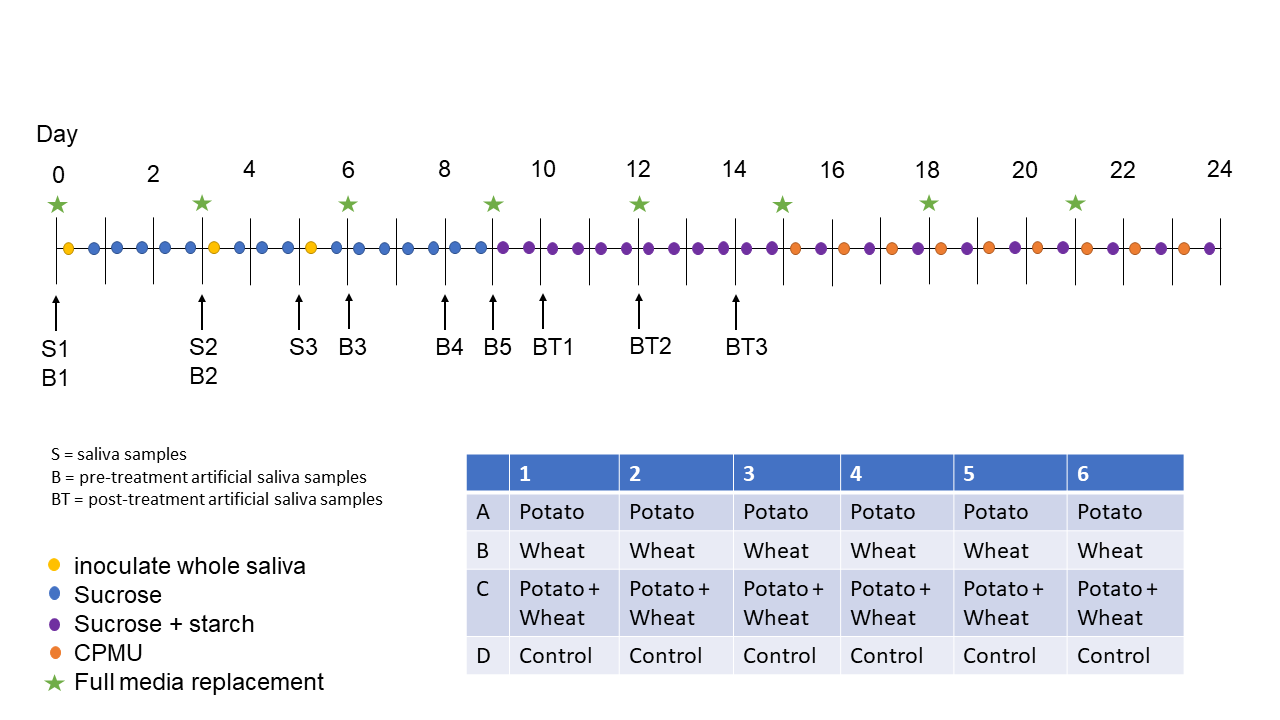
\includegraphics[width=4.27in,height=\textheight]{figures/protocol_overview.png}

}

\caption{\label{fig-protocol}Overview of experiment protocol including
the plate setup.}

\end{figure}%

All laboratory work was conducted in sterile conditions under a laminar
flow hood to prevent starch and bacterial contamination. Control samples
that only received sucrose as a treatment were included to detect starch
contamination from the environment or cross-contamination from other
wells in the same plate.

\subsection{Amylase activity
detection}\label{amylase-activity-detection}

An \(\alpha\)-amylase (EC 3.2.1.1) activity assay was conducted on
artificial saliva samples collected from the plate wells on days 3, 6,
8, 9, 10, 12, and 14. Whole saliva samples were collected on days 0, 3,
and 5 as positive controls. Collected samples were stored at 4°C until
the assay was conducted on day 18. All samples and standard curves were
run in triplicates on two separate plates. Positive control saliva
samples were compared against a standard curve containing
H\textsubscript{2}O, while artificial saliva samples were compared
against a standard curve containing stock AS (due to the colour of
artificial saliva). Two photometric readings were conducted for each
plate with a 540 nm filter on a Multiskan FC Microplate Photometer
(Thermo Scientific 51119000). The protocol is a modified version of an
Enzymatic Assay of \(\alpha\)-Amylase
(\url{https://www.sigmaaldrich.com/NL/en/technical-documents/protocol/protein-biology/enzyme-activity-assays/enzymatic-assay-of-a-amylase})
(\citeproc{ref-bernfeldAmylase1955}{Bernfeld, 1955}), which measures the
amount of maltose released from starch by \(\alpha\)-amylase activity.
Results are reported in units (U) per mL enzyme, where 1 U releases 1
\(\mu\)mole of maltose in 6 minutes. The detailed protocol can be found
here: \url{https://www.protocols.io/view/amylase-activity-bw8jphun}.

\subsection{Treatment solutions}\label{treatment-solutions}

A 1 ml aliquot of each starch solution was taken, from which 10 \(\mu\)l
was mounted on a microscope slide with an 18 x 18 mm coverslip, and
counted under a light microscope (Zeiss Axioscope A1). For wheat and
mixed treatment samples, we counted three slide transects (at ca. 1/4,
1/2, and 3/4 of the slide), and the sample counts were extrapolated to
the total number of granules exposed to the samples over 16 days of
treatments (see Supplementary Material for more details). For potato
treatment samples, the whole slide was counted.

\subsection{Extraction method}\label{extraction-method}

Extraction of starches from the calculus samples was performed by
dissolving the calculus in 0.5 \(\tiny{M}\) ethylenediaminetetraacetic
acid (EDTA) (\citeproc{ref-lemoyneCalculusPretreatments2021}{Le Moyne \&
Crowther, 2021}; \citeproc{ref-modiCalculusMethodologies2020}{Modi et
al., 2020}; \citeproc{ref-trompEDTACalculus2017}{Tromp et al., 2017}),
and vortexing for 3 days until the sample was completely dissolved.
Twenty \(\mu\)l of sample was mounted onto a slide with an 18x18 mm
coverslip. When transferring the sample to the slide, the sample was
homogenised using the pipette to ensure that the counted transects were
representative of the whole slide. The count from the slide was
extrapolated to the whole sample (see Supplementary Material for more
detail).

Both wheat and potato granules were divided into three size categories:
small (\textless10 \(\mu\)m), medium (10 -- 20 \(\mu\)m), and large
(\textgreater20 \(\mu\)m).

\subsection{Statistical analysis}\label{statistical-analysis}

Statistical analysis was conducted in R version 4.3.3 (2024-02-29)
(\citeproc{ref-Rbase}{R Core Team, 2020}) and the following packages:
tidyverse (\citeproc{ref-tidyverse2019}{Wickham et al., 2019}), broom
(\citeproc{ref-Rbroom}{Robinson et al., 2021}), here
(\citeproc{ref-Rhere}{Müller, 2020}), and patchwork
(\citeproc{ref-Rpatchwork}{Pedersen, 2020}).

To see if biofilm growth was differently affected by starch treatments,
a one-way ANOVA with sample weight as the dependent variable (DV) and
treatment as the grouping variable (GV) was conducted. To analyse
granule counts and calculate size proportions, mean counts for each
treatment were taken across both experimental plates, resulting in a
mean count for each granule size category within each treatment.

Pearson's \emph{r} was conducted on sample weight and total starch
count, as well as sample weight and starch count per mg calculus. The
total count for each sample within a treatment was standardised by
z-score to account for the differences in magnitude between the potato
and wheat counts. This was applied to total biofilm weight and starch
count per mg calculus (also z-score standardised) to account for
differences in starch concentration in the calculus (as per
\citeproc{ref-wesolowskiEvaluatingMicrofossil2010}{Wesolowski et al.,
2010}).

\section{Results}\label{results-1}

All samples yielded sufficient biofilm growth and starch incorporation
to be included in the analysis (Figure~\ref{fig-microscope}), resulting
in a total of 48 biofilm samples (two plates of 24), 45 of which were
used for analysis (three samples were set aside for later analysis).
Most control samples contained no starch granules, while some contained
negligible quantities (see Supplementary Material).

\begin{figure}

\begin{minipage}{0.50\linewidth}
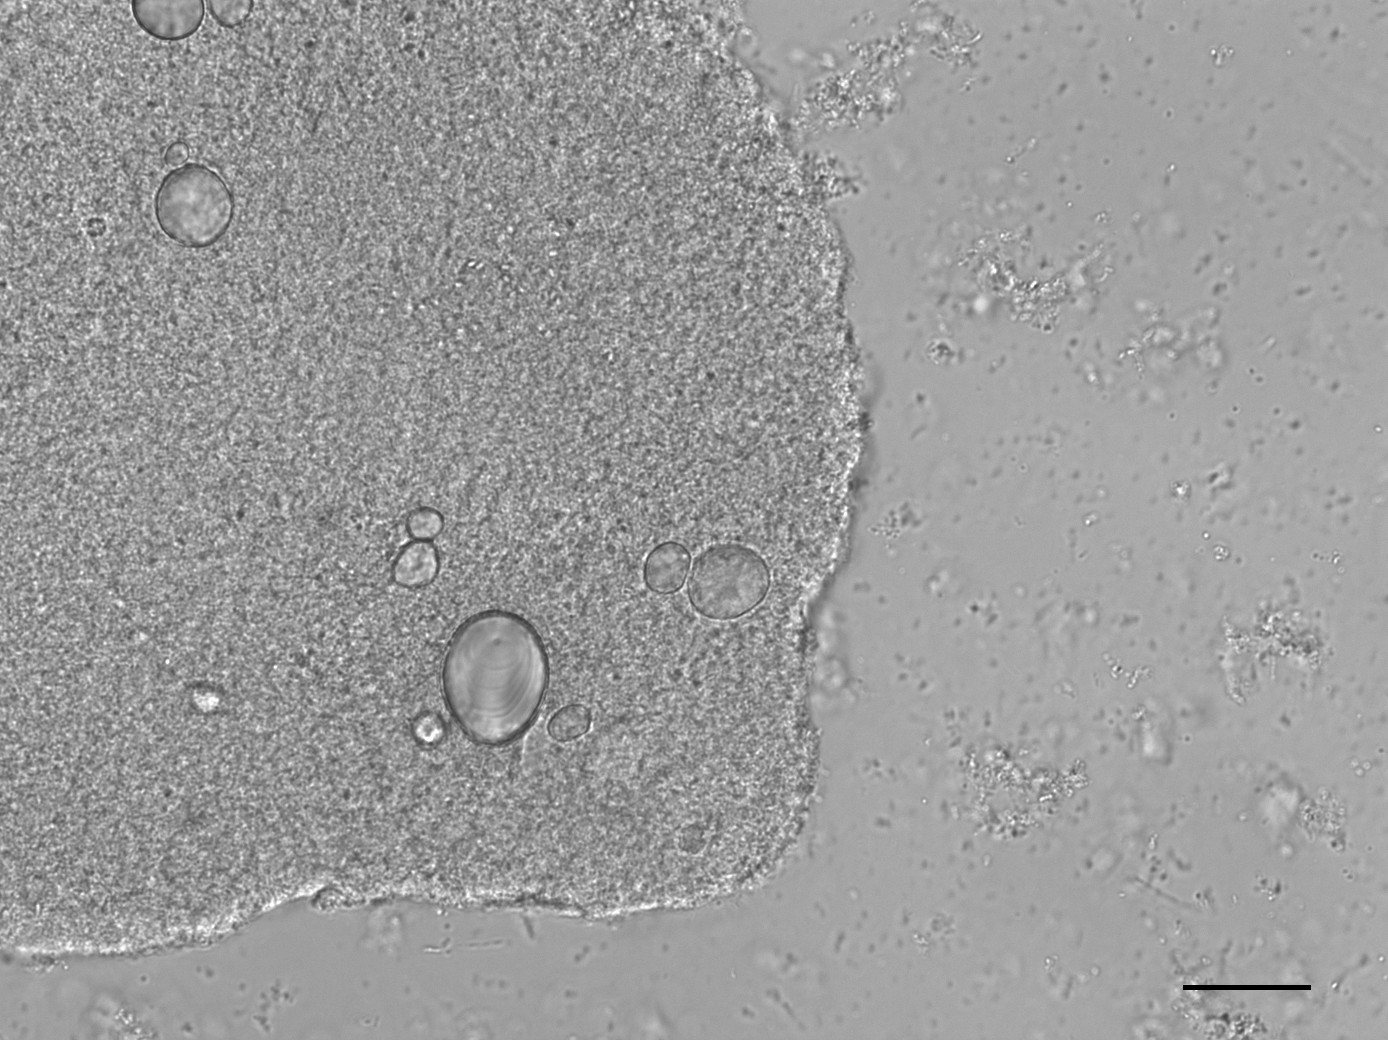
\includegraphics{figures/starches_w_bar.jpg}\end{minipage}%
%
\begin{minipage}{0.50\linewidth}
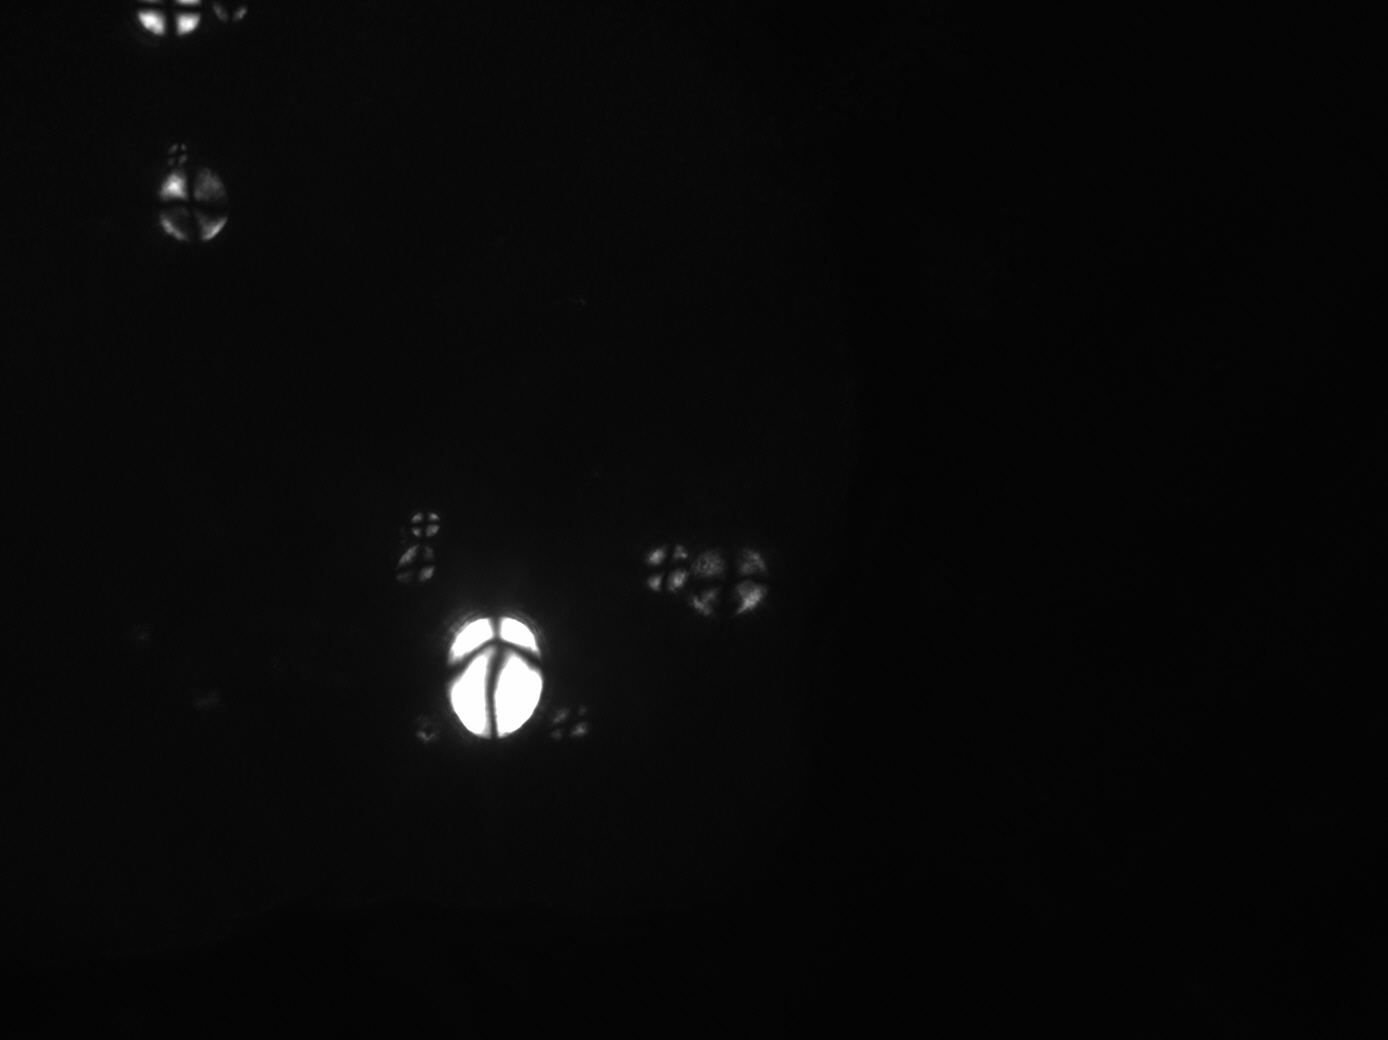
\includegraphics{figures/st2C3.2-mix.jpg}\end{minipage}%
\newline
\begin{minipage}{0.50\linewidth}
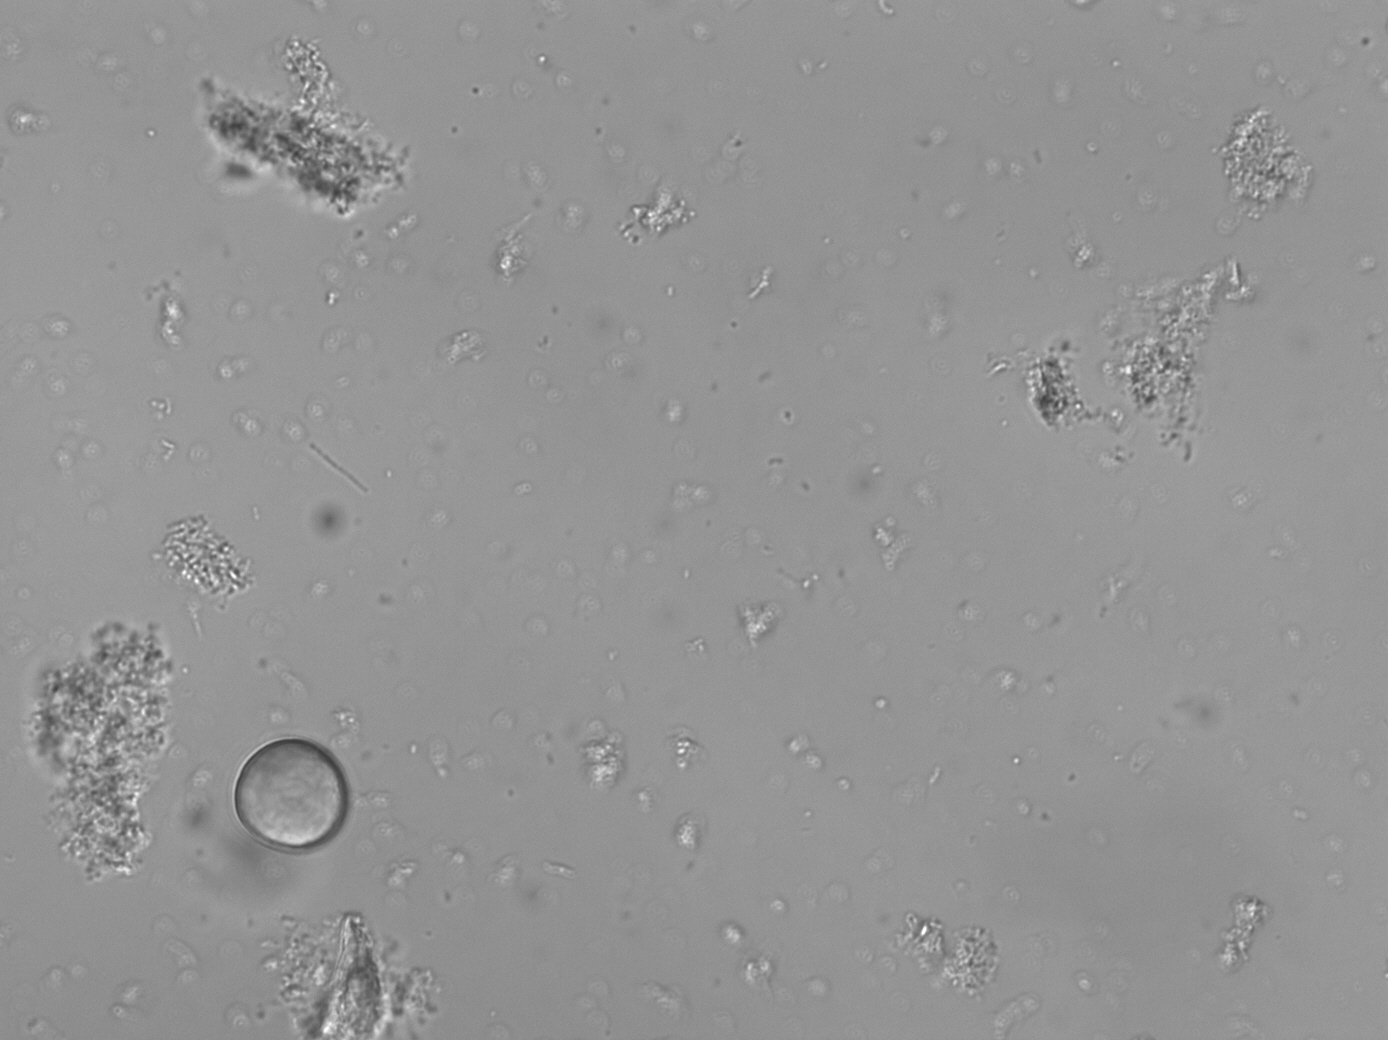
\includegraphics{figures/st1B4-wheat.jpg}\end{minipage}%
%
\begin{minipage}{0.50\linewidth}
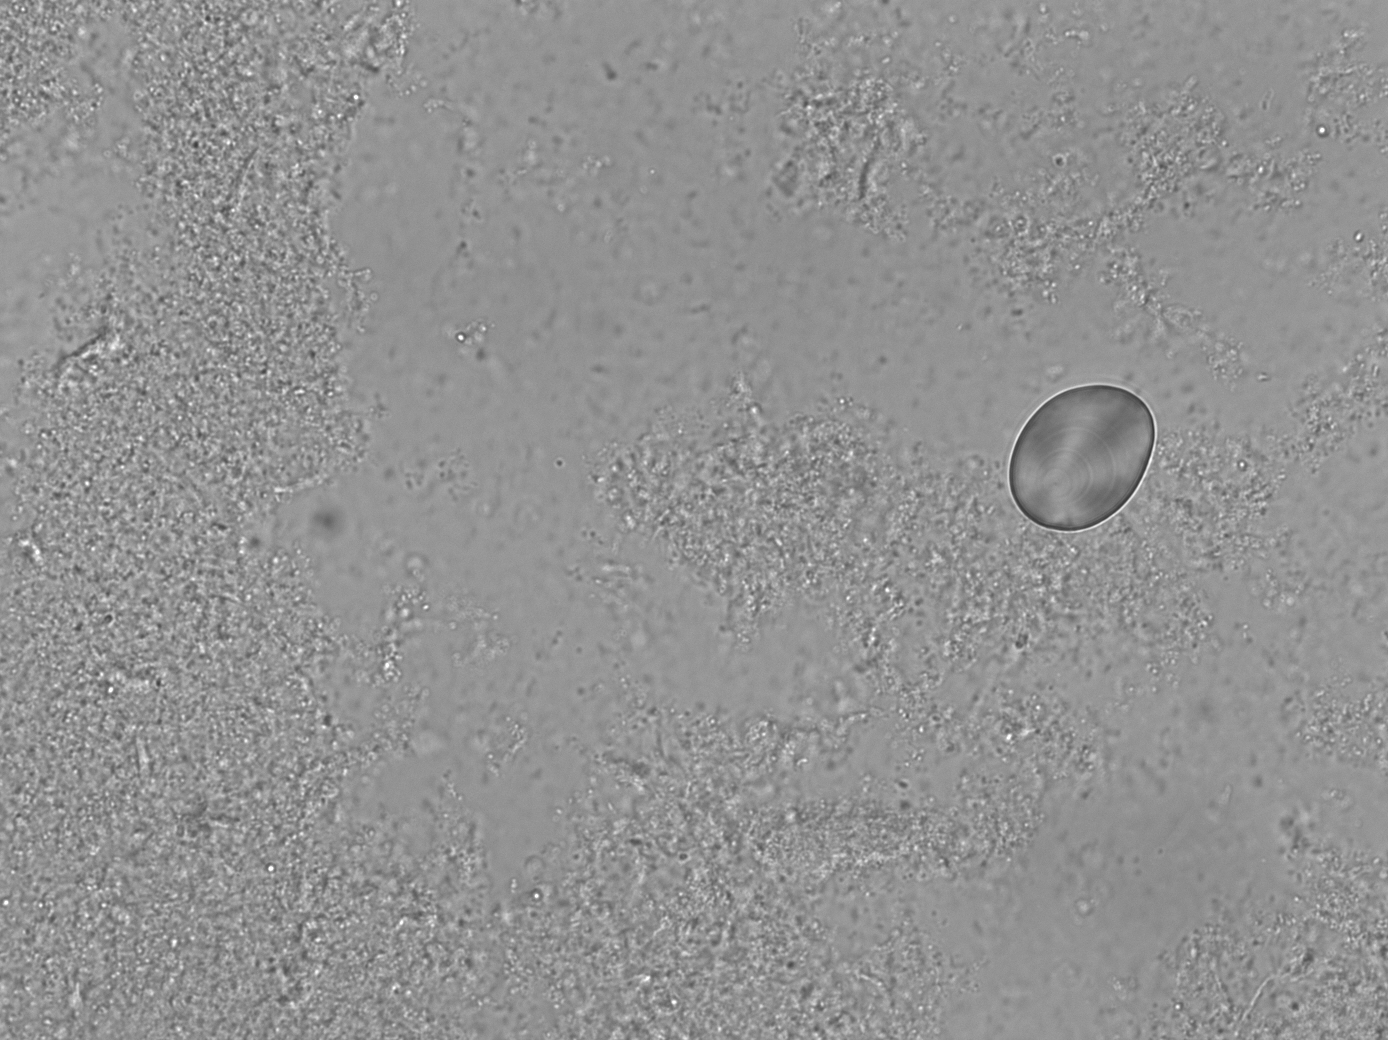
\includegraphics{figures/2D2-potato.jpg}\end{minipage}%

\caption{\label{fig-microscope}Microscope images of biofilm samples that
were exposed to the starch solutions. Starch granules can be seen within
bacterial communities and isolated. Scale bar = 20 μm.}

\end{figure}%

\subsection{No amylase activity detected in the
model}\label{no-amylase-activity-detected-in-the-model}

No \(\alpha\)-amylase activity was detected in any of the artificial
saliva samples from any of the days that were sampled. Only positive
controls (saliva) contained amylase activity that could be detected in
the assay, ranging from 9.93 to 30.2 U/mL enzyme (full results can be
found in the Supplementary Material). The results are not comparable to
other studies presenting \(\alpha\)-amylase activity levels in humans,
as the unit definition may differ; however, they are sufficient to show
that there is no activity in the model.

\subsection{Treatment type had minimal effect on biofilm
growth}\label{treatment-type-had-minimal-effect-on-biofilm-growth}

A one-way ANOVA suggests that the type of starch used during the biofilm
growth period had a minimal effect on the growth of the biofilm
(expressed as total dry weight of the sample), F(3, 43) = 1.16, p =
0.335. A summary of sample weights is available in
Table~\ref{tbl-anova}.

\begin{longtable}[]{@{}lrrrr@{}}

\caption{\label{tbl-anova}Summary statistics for biofilm dry-weights (in
mg) by treatment.}

\tabularnewline

\toprule\noalign{}
Treatment & Mean & SD & Min & Max \\
\midrule\noalign{}
\endhead
\bottomrule\noalign{}
\endlastfoot
control & 5.44 & 2.45 & 1.67 & 11.20 \\
mix & 4.28 & 1.95 & 1.50 & 8.44 \\
potato & 6.25 & 2.07 & 2.54 & 8.92 \\
wheat & 5.53 & 3.45 & 0.56 & 9.80 \\

\end{longtable}

\subsection{Starch counts}\label{starch-counts}

It was not possible to differentiate between potato and wheat starches
smaller than ca. 10 \(\mu\)m. These were counted as wheat, as we assumed
that the majority of the small granules were wheat. We make this
assumption based on the counts of small starches in the wheat-only and
potato-only solutions. Of the combined amount of small starches in these
two solutions, 99.2\% are from wheat.

The separate wheat and potato solutions were made with a 0.25\% (w/v)
starch concentration, while the mixed-starch solution was made with
0.25\% (w/v) of each starch, with a total concentration of 0.50\% (w/v).
The mixed treatment had the highest absolute count of starch granules in
solution (mean = \ensuremath{2.9\times 10^{7}}), while the biofilms
exposed to the wheat solution preserved the greatest number of granules
(mean = \ensuremath{2.77\times 10^{4}}). The potato treatment had the
lowest absolute counts in both the solution
(\ensuremath{3.02\times 10^{6}}) and in the biofilm samples (4850)
(Table~\ref{tbl-solution-count} and Table~\ref{tbl-sample-count}).

\begin{longtable}[]{@{}
  >{\raggedright\arraybackslash}p{(\columnwidth - 10\tabcolsep) * \real{0.1084}}
  >{\raggedright\arraybackslash}p{(\columnwidth - 10\tabcolsep) * \real{0.0843}}
  >{\raggedright\arraybackslash}p{(\columnwidth - 10\tabcolsep) * \real{0.2048}}
  >{\raggedright\arraybackslash}p{(\columnwidth - 10\tabcolsep) * \real{0.1928}}
  >{\raggedright\arraybackslash}p{(\columnwidth - 10\tabcolsep) * \real{0.1928}}
  >{\raggedright\arraybackslash}p{(\columnwidth - 10\tabcolsep) * \real{0.2169}}@{}}

\caption{\label{tbl-solution-count}Mean starch counts from solutions,
including the proportional makeup of the different sizes of granules.}

\tabularnewline

\toprule\noalign{}
\begin{minipage}[b]{\linewidth}\raggedright
Solution
\end{minipage} & \begin{minipage}[b]{\linewidth}\raggedright
Starch
\end{minipage} & \begin{minipage}[b]{\linewidth}\raggedright
Small (\%)
\end{minipage} & \begin{minipage}[b]{\linewidth}\raggedright
Medium (\%)
\end{minipage} & \begin{minipage}[b]{\linewidth}\raggedright
Large (\%)
\end{minipage} & \begin{minipage}[b]{\linewidth}\raggedright
Total (\%)
\end{minipage} \\
\midrule\noalign{}
\endhead
\bottomrule\noalign{}
\endlastfoot
mix & potato & & 1051733 (53.1\%) & 928000 (46.9\%) & 1979733
(100.0\%) \\
mix & wheat & 18838400 (69.7\%) & 6403200 (23.7\%) & 1794133 (6.6\%) &
27035733 (100.0\%) \\
mix & both & 18838400 (64.9\%) & 7454933 (25.7\%) & 2722133 (9.4\%) &
29015467 (100.0\%) \\
potato & potato & 123733 (4.1\%) & 1337867 (44.4\%) & 1554400 (51.5\%) &
3016000 (100.0\%) \\
wheat & wheat & 16139467 (63.5\%) & 6434133 (25.3\%) & 2830400 (11.1\%)
& 25404000 (100.0\%) \\

\end{longtable}

\begin{longtable}[]{@{}
  >{\raggedright\arraybackslash}p{(\columnwidth - 18\tabcolsep) * \real{0.1053}}
  >{\raggedright\arraybackslash}p{(\columnwidth - 18\tabcolsep) * \real{0.0737}}
  >{\raggedright\arraybackslash}p{(\columnwidth - 18\tabcolsep) * \real{0.1579}}
  >{\raggedleft\arraybackslash}p{(\columnwidth - 18\tabcolsep) * \real{0.0632}}
  >{\raggedright\arraybackslash}p{(\columnwidth - 18\tabcolsep) * \real{0.1474}}
  >{\raggedleft\arraybackslash}p{(\columnwidth - 18\tabcolsep) * \real{0.0632}}
  >{\raggedright\arraybackslash}p{(\columnwidth - 18\tabcolsep) * \real{0.1368}}
  >{\raggedleft\arraybackslash}p{(\columnwidth - 18\tabcolsep) * \real{0.0526}}
  >{\raggedright\arraybackslash}p{(\columnwidth - 18\tabcolsep) * \real{0.1368}}
  >{\raggedleft\arraybackslash}p{(\columnwidth - 18\tabcolsep) * \real{0.0632}}@{}}

\caption{\label{tbl-sample-count}Mean starch counts extracted from
samples with standard deviation (SD), including the proportion of
granule sizes of the total count.}

\tabularnewline

\toprule\noalign{}
\begin{minipage}[b]{\linewidth}\raggedright
Treatment
\end{minipage} & \begin{minipage}[b]{\linewidth}\raggedright
Starch
\end{minipage} & \begin{minipage}[b]{\linewidth}\raggedright
Small (\%)
\end{minipage} & \begin{minipage}[b]{\linewidth}\raggedleft
SD
\end{minipage} & \begin{minipage}[b]{\linewidth}\raggedright
Medium (\%)
\end{minipage} & \begin{minipage}[b]{\linewidth}\raggedleft
SD
\end{minipage} & \begin{minipage}[b]{\linewidth}\raggedright
Large (\%)
\end{minipage} & \begin{minipage}[b]{\linewidth}\raggedleft
SD
\end{minipage} & \begin{minipage}[b]{\linewidth}\raggedright
Total (\%)
\end{minipage} & \begin{minipage}[b]{\linewidth}\raggedleft
SD
\end{minipage} \\
\midrule\noalign{}
\endhead
\bottomrule\noalign{}
\endlastfoot
mix & potato & & & 1959 (79.6\%) & 1801 & 501 (20.40\%) & 446 & 2460
(100\%) & 2189 \\
mix & wheat & 9515 (54.60\%) & 8860 & 6522 (37.4\%) & 6026 & 1381
(7.93\%) & 1196 & 17417 (100\%) & 15878 \\
mix & both & 9515 (47.90\%) & 8860 & 8480 (42.7\%) & 7653 & 1882
(9.47\%) & 1596 & 19877 (100\%) & 17768 \\
potato & potato & 351 (7.24\%) & 297 & 3565 (73.6\%) & 2402 & 930
(19.20\%) & 929 & 4846 (100\%) & 3316 \\
wheat & wheat & 15235 (55.00\%) & 11944 & 12148 (43.9\%) & 11052 & 1953
(7.06\%) & 2016 & 27680 (100\%) & 23554 \\

\end{longtable}

\subsubsection{Proportion of available starches incorporated in
samples}\label{proportion-of-available-starches-incorporated-in-samples}

The proportion of total starches from the solutions that were
incorporated into the samples ranged from 0.06\% to 0.16\%, with potato
granules being more readily incorporated than wheat in both the
separated- and mixed-treatment samples (Table~\ref{tbl-sample-prop}).
There is an inverse relationship between the absolute starch count in
the solutions and the proportional incorporation of starches in the
biofilm samples, i.e., potato had the lowest absolute count in
solutions, but the highest proportional incorporation, and vice versa
for the mixed treatment.

\begin{longtable}[]{@{}llllll@{}}

\caption{\label{tbl-sample-prop}The mean percentage of starches from the
solutions that were incorporated into the samples.}

\tabularnewline

\toprule\noalign{}
Treatment & Starch & Small & Medium & Large & Total \\
\midrule\noalign{}
\endhead
\bottomrule\noalign{}
\endlastfoot
mix & potato & & 0.19\% & 0.05\% & 0.12\% \\
mix & wheat & 0.05\% & 0.10\% & 0.08\% & 0.06\% \\
mix & both & 0.05\% & 0.11\% & 0.07\% & 0.07\% \\
potato & potato & 0.28\% & 0.27\% & 0.06\% & 0.16\% \\
wheat & wheat & 0.09\% & 0.19\% & 0.07\% & 0.12\% \\

\end{longtable}

Wheat incorporation was most affected in the mixed-treatment samples,
with only 0.06\% of the total available starches being incorporated into
the sample, compared to 0.16\% in the separated wheat treatment.

\subsubsection{Size ratios differ between solutions and
samples}\label{size-ratios-differ-between-solutions-and-samples}

Overall, medium starch granules had a higher mean rate of incorporation
(0.171\%) than small (0.120\%) and large (0.066\%) starch granules
across all treatments, while large potato starches had the lowest rate
of incorporation across all treatments.

The difference in incorporation between the size categories resulted in
a change in size ratios between the original starch solutions and the
extracted samples. Large potato granules (\textgreater{} 20 \(\mu\)m)
were most affected, with a 32.3\% decrease in relative abundance in the
potato-only treatment, and a 26.5\% decrease in mixed treatments. Medium
granules increased in relative abundance across all samples, while small
granules decreased in wheat treatments and increased in potato
treatments (Figure~\ref{fig-ratio-plots}).

\begin{figure}[H]

\centering{

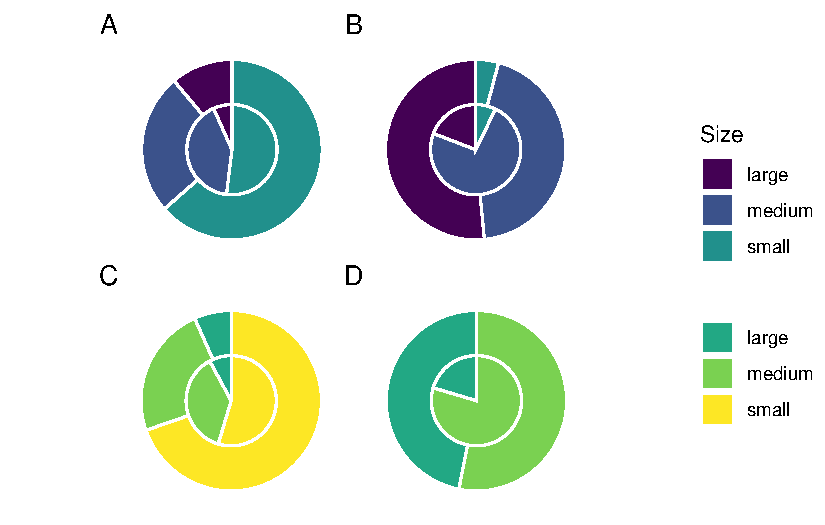
\includegraphics{figures/byoc-starch-fig-ratio-plots-1.pdf}

}

\caption{\label{fig-ratio-plots}Proportion of sizes of starch granules
from solutions (outer ring) and treatment samples (inner ring) in
separated wheat (A) and potato (B) treatments, and mixed wheat (C) and
potato (D) treatments.}

\end{figure}%

\subsubsection{Biofilm weight correlated positively with extracted
starch
counts}\label{biofilm-weight-correlated-positively-with-extracted-starch-counts}

Pearson's \emph{r} suggests a strong positive correlation between the
total weight of the biofilms and the total starch count (standardised by
z-score) extracted from the samples across treatments, \emph{r} = 0.659,
90\%CI{[}0.463, 0.794{]}, p \textless{} 0.001
(Figure~\ref{fig-cor-plot}A).

\begin{figure}[H]

\centering{

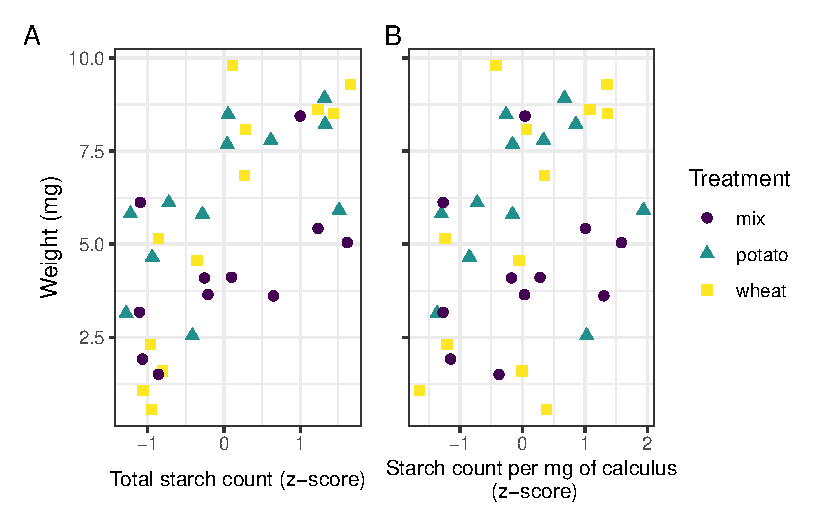
\includegraphics{figures/byoc-starch-fig-cor-plot-1.pdf}

}

\caption{\label{fig-cor-plot}Scatter plots of (A) sample weight in mg
and standardised starch count by z-score for separated treatments, and
(B) sample weight in mg and standardised count of starch grains per mg
calculus.}

\end{figure}%

The same test was applied to total biofilm weight and starch count per
mg calculus (also standardised by z-score), resulting in a weak positive
correlation, \emph{r} = 0.3, 90\%CI{[}0.0618, 0.506{]}, p = 0.0403
(Figure~\ref{fig-cor-plot}B).

\section{Discussion}\label{discussion-1}

Here, we have provided a method for exploring the incorporation of
dietary starches into the mineral matrix of a dental calculus biofilm
model. Our results show that a very low proportion of the starches
exposed to the biofilm during growth are retained in the mineral matrix,
and that the size of the starch granules may affect the likelihood of
incorporation. The proportions of starch granules (of all sizes) present
in the extracted samples were similar across all treatments (0.06\% to
0.16\%), despite large differences in absolute granule counts between
wheat (mean = 25,404,000) and potato (mean = 3,016,000) solutions.\\
The absolute counts, however, differed more visibly between treatments
and was proportional with the total count of granules in the treatment
solutions. Wheat and mixed solutions had the highest absolute mean count
of starch granules, and also had the highest absolute mean count of
starch granules extracted from the dental calculus
(Table~\ref{tbl-solution-count} and Table~\ref{tbl-sample-count}). This
suggests that the starches that are more frequently consumed will be
present in higher quantities in the dental calculus, at least prior to
inhumation and degradation in the burial environment. Despite the low
proportion of granules recovered from the model calculus (0.06\% to
0.16\%), the absolute counts were still substantially greater than
counts recovered from archaeological remains
(\citeproc{ref-trompEDTACalculus2017}{Tromp et al., 2017};
\citeproc{ref-trompDietaryNondietary2015}{Tromp \& Dudgeon, 2015};
\citeproc{ref-wesolowskiEvaluatingMicrofossil2010}{Wesolowski et al.,
2010}), which could in part be due to the lack of oral amylase activity
in our model. Previous research conducted on dental calculus from
contemporary humans and non-human primates suggest a high level of
stochasticity involved in the retention of starch granules in dental
calculus, and that starch granules extracted from dental calculus are
underrepresented with regard to actual starch intake, which is
consistent with our findings (illustrated by high standard deviations
and low proportional incorporation). Leonard and colleagues
(\citeproc{ref-leonardPlantMicroremains2015}{2015}) found individual
calculus samples to be a poor predictor of diet in a population, as many
of the consumed plants were missing from some individual samples, but
were present in others.\\
Power and colleagues (\citeproc{ref-powerChimpCalculus2015}{2015})
presented similar findings in non-human primates, where phytoliths were
more representative of individual diets than starch granules. The size
bias is also consistent with the findings by Power and colleagues
(\citeproc{ref-powerChimpCalculus2015}{2015}), who found that plants
producing starches 10--20 \(\mu\)m in size were over-represented;
however, the representation of granules larger than 20 \(\mu\)m in their
study is unclear.

We have also shown that the size of the starch granules influences the
likelihood of incorporation into the calculus. Starch granules larger
than 20 \(\mu\)m in maximum length were underrepresented in the calculus
samples compared to the original starch solutions, an effect that was
consistent across all three treatments. Medium granules (10--20
\(\mu\)m) were often over-represented (Table~\ref{tbl-sample-prop}, and
Figure~\ref{fig-ratio-plots}). Large potato granules were most affected,
potentially because of the greater size-range. They can reach up to 100
\(\mu\)m in maximum length, whereas wheat granules generally only reach
up to 35 \(\mu\)m (\citeproc{ref-gismondiStarchGranules2019}{Gismondi et
al., 2019}; \citeproc{ref-haslamDecompositionStarch2004}{Haslam, 2004};
\citeproc{ref-seidemannStarchAtlas1966}{Seidemann, 1966, pp. 174--176}).
Granule morphology may also play a role. Large wheat granules are
lenticular and have a larger surface area compared to volume, whereas
large potato granules are ovoid and have a larger volume compared to
surface area (\citeproc{ref-janeAnthologyStarch1994}{Jane et al., 1994};
\citeproc{ref-reichertStarchBible1913b}{Reichert, 1913, pp. 364--365};
\citeproc{ref-seidemannStarchAtlas1966}{Seidemann, 1966, pp. 174--176};
\citeproc{ref-vandeveldeStarchMorphology2002}{van de Velde et al.,
2002}). Another potentially important factor from our results is the
size of the calculus deposit. We found a strong positive correlation
between size of biofilm deposit and retained starch granules
(Figure~\ref{fig-cor-plot}A), meaning larger calculus deposits contain a
higher quantity of granules; a result that contradicts findings from
archaeological contexts (\citeproc{ref-dudgeonDietGeography2014}{Dudgeon
\& Tromp, 2014};
\citeproc{ref-wesolowskiEvaluatingMicrofossil2010}{Wesolowski et al.,
2010}). When the concentration of starch granules per mg calculus is
considered, the correlation is weaker, but still present
(Figure~\ref{fig-cor-plot}B). While the larger deposits contain a higher
absolute count, our findings also suggest that they contain a slightly
higher concentration of starches. This may also explain the lower mean
retention of starch granules in mixed treatments compared to wheat
treatments. Wheat treatment samples (mean = 5.53 mg) were on average
larger than mixed treatment samples (mean = 4.28 mg)
(Table~\ref{tbl-anova}); and while mixed treatment solutions contained
the highest mean overall granule counts, wheat treatment samples had the
highest mean starch retention. Further research is needed to determine
why this differs from previous archaeological findings.

The mechanism by which starch granules are incorporated into plaque and
calculus remains largely unknown, and few studies have directly
investigated potential mechanisms. We know that a proportion of the
starch granules entering the mouth can become trapped in the
plaque/calculus, and can be recovered from archaeological samples of
considerable age (\citeproc{ref-buckleyDentalCalculus2014}{Buckley et
al., 2014}; \citeproc{ref-henryNeanderthalCalculus2014}{Henry et al.,
2014}; \citeproc{ref-wuDietEarliest2021}{Wu et al., 2021}). Studies have
also shown that not all starch granules come from a dietary source.
Other pathways include cross-contamination from plant interactions in
soil, such as palm phytoliths adhering to the skin of sweet potatoes
(\citeproc{ref-trompDietaryNondietary2015}{Tromp \& Dudgeon, 2015}), or
accidental ingestion not related to food consumption
(\citeproc{ref-radiniFoodPathways2017}{Radini et al., 2017},
\citeproc{ref-radiniMedievalWomen2019}{2019}).\\
When starch granules enter the mouth, whether through ingestion of food
or accidental intake, they immediately encounter multiple obstacles. It
is likely that the bulk of starch granules are swallowed along with the
food, and are only briefly present in the oral cavity. Other granules
that are broken off during mastication may be retained in the dentition
through attachment to tooth surfaces (including plaque and dental
calculus) and mucous membranes
(\citeproc{ref-doddsCarbohydrateRetention1988}{Dodds \& Edgar, 1988};
\citeproc{ref-kashketFoodRetention1991}{S. Kashket et al., 1991}).
Bacteria also have the ability to adhere to starch granules
(\citeproc{ref-toppingResistantStarch2003}{Topping et al., 2003}), which
would allow starches to attach to bacterial communities within the
biofilm. These granules are then susceptible to mechanical removal by
the tongue, salivary clearance, and hydrolysis by \(\alpha\)-amylase
(\citeproc{ref-kashketFoodParticles1996}{S. Kashket et al., 1996}). The
susceptibility of granules to hydrolysis depends on the crystallinity
and size of the starch granule, as well as the mode of processing.
Smaller and pre-processed (e.g., cooked) starch granules are more
susceptible to enzymatic degradation, while dehydrated starches will
have a reduced susceptibility
(\citeproc{ref-bjorckStarchProcessing1984}{Björck et al., 1984};
\citeproc{ref-francoStarchDegradation1992}{Franco et al., 1992};
\citeproc{ref-haslamDecompositionStarch2004}{Haslam, 2004};
\citeproc{ref-henryCookingStarch2009}{Henry et al., 2009};
\citeproc{ref-lingstromStarchyFood1994}{Lingstrom et al., 1994}). Cracks
on the surface of the dental calculus, as well as unmineralised islands
and channels may also be able to contain starch granules
(\citeproc{ref-charlierSEMCalculus2010}{Charlier et al., 2010};
\citeproc{ref-powerSEMCalculus2014}{R. C. Power et al., 2014};
\citeproc{ref-tanCalculusUltrastructure2004}{Tan, Gillam, et al.,
2004}). Starch granules that are trapped in these pockets are (at least
to some extent) protected from aforementioned clearance mechanisms,
especially once a new layer of plaque has covered the surface of the
plaque/calculus. The size bias against large granules (\textgreater20
\(\mu\)m) from both wheat and potato (Table~\ref{tbl-sample-prop}) may
give further credence to this incorporation pathway, as the smaller
starch granules have an advantage over larger granules, and can be
stored in larger quantities. This was also suggested by Power and
colleagues (\citeproc{ref-powerSEMCalculus2014}{2014}), who observed
clusters of starches within dental calculus, rather than an even
distribution across the surface of the dental calculus. Granules trapped
in plaque/calculus may still be susceptible to hydrolysis, as
\(\alpha\)-amylase has the ability to bind to both tooth enamel and
bacteria within a biofilm and retain a portion of its hydrolytic
activity (\citeproc{ref-nikitkovaStarchBiofilms2013}{Nikitkova et al.,
2013}; \citeproc{ref-scannapiecoSalivaryAmylase1993}{Scannapieco et al.,
1993}; \citeproc{ref-tanBacterialViability2004}{Tan, Mordan, et al.,
2004}; \citeproc{ref-tanCalculusUltrastructure2004}{Tan, Gillam, et al.,
2004}). After the death of an individual, starches within dental
calculus are susceptible to further degradation by post-depositional
processes, depending on burial environment (pH, temperature, moisture
content, microorganisms)
(\citeproc{ref-francoStarchDegradation1992}{Franco et al., 1992};
\citeproc{ref-graneroStarchTaphonomy2020}{García-Granero, 2020};
\citeproc{ref-haslamDecompositionStarch2004}{Haslam, 2004};
\citeproc{ref-henryCookingStarch2009}{Henry et al., 2009}). Future study
should explore how burial affects the recovery of starch from the
biofilm model.

The absence of \(\alpha\)-amylase in the model is a limitation of this
study, as the total granule counts were not subject to hydrolysis. This
would likely have reduced and affected the size ratios, as smaller
starches may be more susceptible to hydrolysis
(\citeproc{ref-francoStarchDegradation1992}{Franco et al., 1992};
\citeproc{ref-haslamDecompositionStarch2004}{Haslam, 2004}). The absence
may also affect biofilm growth due to the lack of amylase-bacterium
interactions (\citeproc{ref-nikitkovaStarchBiofilms2013}{Nikitkova et
al., 2013}). Conversely, the model may benefit from the absence of
\(\alpha\)-amylase, because it can allow us to directly explore its
effect on starch counts in future experiments, where \(\alpha\)-amylase
can be added to the model in concentrations similar to those found in
the oral cavity
(\citeproc{ref-scannapiecoSalivaryAmylase1993}{Scannapieco et al.,
1993}). We are able to show how absolute counts in the treatments cause
a difference in incorporation. However, this was merely a side-effect of
the difference in the number of granules in potato and wheat solutions
of the same concentration (w/v). Further research should test multiple
differing concentrations of the same starch type. The use of EDTA may
also have affected counts. While previous studies have shown negligible
morphological changes caused by exposure to EDTA
(\citeproc{ref-lemoyneCalculusPretreatments2021}{Le Moyne \& Crowther,
2021}; \citeproc{ref-modiCalculusMethodologies2020}{Modi et al., 2020};
\citeproc{ref-trompEDTACalculus2017}{Tromp et al., 2017}), these studies
have not considered changes to separate size categories within starch
types, and whether shifts in size ratios occur due to exposure to the
pre-treatment chemicals. The total number of granules on a slide often
exceeded a number that was feasible to count in a reasonable time
period, so we calculated the total counts by extrapolating from three
slide transects. Thus, we reasonably assume that the three transects are
a good representation of the entire slide, and that the distribution of
all granules on the slide is relatively homogeneous.\\
Finally, we only used native starches in the experimental procedure and
the results will likely differ for processed starches
(\citeproc{ref-graneroStarchTaphonomy2020}{García-Granero, 2020}). Based
on the comparatively low counts obtained by Leonard and colleagues
(\citeproc{ref-leonardPlantMicroremains2015}{2015}, Supplement 2),
processing and amylase may have a substantial effect on starch granule
retention in the oral cavity.

While we are unable to sufficiently address the mechanism(s) of starch
incorporation with the data obtained in this study, the dental calculus
model presented here is uniquely suited to explore these questions and
may improve interpretations of dietary practices in past populations.
Further analyses using this model can address the call for more baseline
testing of biases associated with dietary research conducted on dental
calculus (\citeproc{ref-lemoyneCalculusPretreatments2021}{Le Moyne \&
Crowther, 2021}). Our high-throughput experimental setup allows us a
higher degree of control over the factors that influence starch
incorporation and retention, such as dietary intake, differential
survivability of starches, and inter- and intra-individual variation in
plaque accumulation and mineralisation. The latter is especially
difficult to control \emph{in vivo} as it is influenced by numerous
factors including genetics, diet, salivary flow, and tooth position and
morphology (\citeproc{ref-fagernasMicrobialBiogeography2021}{Fagernäs et
al., 2021}; \citeproc{ref-haffajeeBiofilmPosition2009}{Haffajee et al.,
2009}; \citeproc{ref-jepsenCalculusRemoval2011}{Jepsen et al., 2011};
\citeproc{ref-proctorSpatialGradient2018}{Proctor et al., 2018};
\citeproc{ref-simonsoroOralGeography2013}{Simón-Soro et al., 2013}), as
well as evolutionary differences
(\citeproc{ref-yatesOralMicrobiome2021}{Fellows Yates et al., 2021}).
The set of limitations for our model differ from \emph{in vivo} methods
and, as such, we expect our model to complement the results and
interpretations of existing and new \emph{in vivo} studies. It can also
facilitate training of students and researchers on methods of dental
calculus analysis, such as starch and phytolith extraction and
identification, where it can replace the use of finite archaeological
resources.

\section{Conclusion}\label{conclusion}

This preliminary study shows that a very small proportion of the input
starch granules are retained in a dental calculus model. This and
previous studies have shown that calculus has a low capacity for
retention of starch granules, an effect that is compounded by diagenetic
effects in archaeological remains, resulting in low overall counts of
extracted granules. The proportion of starches consumed will in many
cases be reflected in the quantity of starches extracted from the dental
calculus---i.e., the more starch granules entering the oral cavity, the
more will be recovered from extraction---at least in modern calculus
samples unaffected by diagenesis and hydrolysis. Whether or not this
also applies to archaeological samples remains to be tested.
Additionally, we have shown that the size of granules will influence the
likelihood of incorporation, as large (\textgreater20 \(\mu\)m) starches
have a decreased incorporation rate, medium (10--20 \(\mu\)m) starches
an increased rate, and small (\textless10 \(\mu\)m) granules remained
somewhat constant. The size of calculus deposit also seems to influence
the capacity of granule incorporation; as the size of the deposit
increases, so does the absolute count of incorporated granules.\\
While we have shown multiple factors that influence the likelihood of
incorporation, the process still appears to be somewhat stochastic.
Further research is needed to make sense of the contributing factors,
and to explore the mechanisms of intra-oral starch incorporation and
retention in dental calculus. The oral biofilm model described in this
study provides a method to explore the incorporation and extraction of
dietary compounds from dental calculus in a controlled laboratory
setting. We do not expect our model to replace \emph{in vivo} methods;
instead, it can provide a complementary means to address the limitations
of \emph{in vivo} studies, and unearth the potential biases associated
with dietary research conducted on archaeological dental calculus.

\section*{References cited}\label{references-cited-3}
\addcontentsline{toc}{section}{References cited}

\markright{References cited}

\phantomsection\label{refs-4}
\begin{CSLReferences}{1}{0}
\bibitem[\citeproctext]{ref-adlerSequencingAncient2013}
Adler, C. J., Dobney, K., Weyrich, L. S., Kaidonis, J., Walker, A. W.,
Haak, W., Bradshaw, C. J., Townsend, G., Sołtysiak, A., Alt, K. W.,
Parkhill, J., \& Cooper, A. (2013). Sequencing ancient calcified dental
plaque shows changes in oral microbiota with dietary shifts of the
{Neolithic} and {Industrial} revolutions. \emph{Nature Genetics},
\emph{45}(4), 450--455, 455e1. \url{https://doi.org/10.1038/ng.2536}

\bibitem[\citeproctext]{ref-armitageExtractionIdentification1975}
Armitage, P. L. (1975). The {Extraction} and {Identification} of {Opal
Phytoliths} from the {Teeth} of {Ungulates}. \emph{Journal of
Archaeological Science}, \emph{2}, 187--197.

\bibitem[\citeproctext]{ref-bernfeldAmylase1955}
Bernfeld, P. (1955). Amylases, {\(\alpha\)} and {\(\beta\)}. In
\emph{Methods in {Enzymology}} (Vol. 1, pp. 149--158). {Academic Press}.
\url{https://doi.org/10.1016/0076-6879(55)01021-5}

\bibitem[\citeproctext]{ref-bjorckStarchProcessing1984}
Björck, I., Asp, N.-G., Birkhed, D., Eliasson, A.-C., Sjöberg, L.-B., \&
Lundquist, I. (1984). Effects of processing on starch availability {In}
vitro and {In} vivo. {II}. {Drum-drying} of wheat flour. \emph{Journal
of Cereal Science}, \emph{2}(3), 165--178.
\url{https://doi.org/10.1016/S0733-5210(84)80030-2}

\bibitem[\citeproctext]{ref-buckleyDentalCalculus2014}
Buckley, S., Usai, D., Jakob, T., Radini, A., \& Hardy, K. (2014).
Dental {Calculus Reveals Unique Insights} into {Food Items}, {Cooking}
and {Plant Processing} in {Prehistoric Central Sudan}. \emph{PLOS ONE},
\emph{9}(7), e100808. \url{https://doi.org/10.1371/journal.pone.0100808}

\bibitem[\citeproctext]{ref-charlierSEMCalculus2010}
Charlier, P., Huynh-Charlier, I., Munoz, O., Billard, M., Brun, L., \&
Grandmaison, G. L. de la. (2010). The microscopic (optical and {SEM})
examination of dental calculus deposits ({DCD}). {Potential} interest in
forensic anthropology of a bio-archaeological method. \emph{Legal
Medicine}, \emph{12}(4), 163--171.
\url{https://doi.org/10.1016/j.legalmed.2010.03.003}

\bibitem[\citeproctext]{ref-doddsCarbohydrateRetention1988}
Dodds, M. W. J., \& Edgar, W. M. (1988). The {Relationship Between
Plaque pH}, {Plaque Acid Anion Profiles}, and {Oral Carbohydrate
Retention After Ingestion} of {Several} '{Reference Foods}' by {Human
Subjects}. \emph{Journal of Dental Research}, \emph{67}(5), 861--865.
\url{https://doi.org/10.1177/00220345880670051301}

\bibitem[\citeproctext]{ref-dudgeonDietGeography2014}
Dudgeon, J. V., \& Tromp, M. (2014). Diet, {Geography} and {Drinking
Water} in {Polynesia}: {Microfossil Research} from {Archaeological Human
Dental Calculus}, {Rapa Nui} ({Easter Island}). \emph{International
Journal of Osteoarchaeology}, \emph{24}(5), 634--648.
\url{https://doi.org/10.1002/oa.2249}

\bibitem[\citeproctext]{ref-eerkensDentalCalculus2018}
Eerkens, J. W., Tushingham, S., Brownstein, K. J., Garibay, R., Perez,
K., Murga, E., Kaijankoski, P., Rosenthal, J. S., \& Gang, D. R. (2018).
Dental calculus as a source of ancient alkaloids: {Detection} of
nicotine by {LC-MS} in calculus samples from the {Americas}.
\emph{Journal of Archaeological Science: Reports}, \emph{18}, 509--515.
\url{https://doi.org/10.1016/j.jasrep.2018.02.004}

\bibitem[\citeproctext]{ref-fagernasMicrobialBiogeography2021}
Fagernäs, Z., Salazar-García, D. C., Avilés, A., Haber, M., Henry, A.,
Maurandi, J. L., Ozga, A., Velsko, I. M., \& Warinner, C. (2021).
Understanding the microbial biogeography of ancient human dentitions to
guide study design and interpretation. \emph{bioRxiv},
2021.08.16.456492. \url{https://doi.org/10.1101/2021.08.16.456492}

\bibitem[\citeproctext]{ref-yatesOralMicrobiome2021}
Fellows Yates, J. A., Velsko, I. M., Aron, F., Posth, C., Hofman, C. A.,
Austin, R. M., Parker, C. E., Mann, A. E., Nägele, K., Arthur, K. W.,
Arthur, J. W., Bauer, C. C., Crevecoeur, I., Cupillard, C., Curtis, M.
C., Dalén, L., Bonilla, M. D.-Z., Fernández-Lomana, J. C. D., Drucker,
D. G., \ldots{} Warinner, C. (2021). The evolution and changing ecology
of the {African} hominid oral microbiome. \emph{Proceedings of the
National Academy of Sciences}, \emph{118}(20).
\url{https://doi.org/10.1073/pnas.2021655118}

\bibitem[\citeproctext]{ref-foxPhytolithCalculus1996}
Fox, C. L., Juan, J., \& Albert, R. M. (1996). Phytolith analysis on
dental calculus, enamel surface, and burial soil: {Information} about
diet and paleoenvironment. \emph{American Journal of Physical
Anthropology}, \emph{101}(1), 101--113.
\url{https://doi.org/10.1002/(SICI)1096-8644(199609)101:1\%3C101::AID-AJPA7\%3E3.0.CO;2-Y}

\bibitem[\citeproctext]{ref-francoStarchDegradation1992}
Franco, C. M. L., Preto, S. J. do R., \& Ciacco, C. F. (1992). Factors
that {Affect} the {Enzymatic Degradation} of {Natural Starch Granules}
-{Effect} of the {Size} of the {Granules}. \emph{Starch - Stärke},
\emph{44}(11), 422--426. \url{https://doi.org/10.1002/star.19920441106}

\bibitem[\citeproctext]{ref-froehlichEffectOral1987}
Froehlich, D. A., Pangborn, R. M., \& Whitaker, J. R. (1987). The effect
of oral stimulation on human parotid salivary flow rate and
alpha-amylase secretion. \emph{Physiology \& Behavior}, \emph{41}(3),
209--217. \url{https://doi.org/10.1016/0031-9384(87)90355-6}

\bibitem[\citeproctext]{ref-graneroStarchTaphonomy2020}
García-Granero, J. J. (2020). Starch taphonomy, equifinality and the
importance of context: {Some} notes on the identification of food
processing through starch grain analysis. \emph{Journal of
Archaeological Science}, \emph{124}, 105267.
\url{https://doi.org/10.1016/j.jas.2020.105267}

\bibitem[\citeproctext]{ref-gismondiStarchGranules2019}
Gismondi, A., D'Agostino, A., Canuti, L., Di Marco, G., Basoli, F., \&
Canini, A. (2019). Starch granules: A data collection of 40 food
species. \emph{Plant Biosystems - An International Journal Dealing with
All Aspects of Plant Biology}, \emph{153}(2), 273--279.
\url{https://doi.org/10.1080/11263504.2018.1473523}

\bibitem[\citeproctext]{ref-haffajeeBiofilmPosition2009}
Haffajee, A. D., Teles, R. P., Patel, M. R., Song, X., Yaskell, T., \&
Socransky, S. S. (2009). Factors affecting human supragingival biofilm
composition. {II}. {Tooth} position. \emph{Journal of Periodontal
Research}, \emph{44}(4), 520--528.
\url{https://doi.org/10.1111/j.1600-0765.2008.01155.x}

\bibitem[\citeproctext]{ref-hardyStarchGranules2009}
Hardy, K., Blakeney, T., Copeland, L., Kirkham, J., Wrangham, R., \&
Collins, M. (2009). Starch granules, dental calculus and new
perspectives on ancient diet. \emph{Journal of Archaeological Science},
\emph{36}(2), 248--255. \url{https://doi.org/10.1016/j.jas.2008.09.015}

\bibitem[\citeproctext]{ref-hardyNeanderthalMedics2012}
Hardy, K., Buckley, S., Collins, M. J., Estalrrich, A., Brothwell, D.,
Copeland, L., García-Tabernero, A., García-Vargas, S., de la Rasilla,
M., Lalueza-Fox, C., Huguet, R., Bastir, M., Santamaría, D., Madella,
M., Wilson, J., Cortés, Á. F., \& Rosas, A. (2012). Neanderthal medics?
{Evidence} for food, cooking, and medicinal plants entrapped in dental
calculus. \emph{Naturwissenschaften}, \emph{99}(8), 617--626.
\url{https://doi.org/10.1007/s00114-012-0942-0}

\bibitem[\citeproctext]{ref-hardyRecoveringInformation2018}
Hardy, K., Buckley, S., \& Copeland, L. (2018). Pleistocene dental
calculus: {Recovering} information on {Paleolithic} food items,
medicines, paleoenvironment and microbes. \emph{Evolutionary
Anthropology: Issues, News, and Reviews}, \emph{27}(5), 234--246.
\url{https://doi.org/10.1002/evan.21718}

\bibitem[\citeproctext]{ref-haslamDecompositionStarch2004}
Haslam, M. (2004). The decomposition of starch grains in soils:
Implications for archaeological residue analyses. \emph{Journal of
Archaeological Science}, \emph{31}(12), 1715--1734.
\url{https://doi.org/10.1016/j.jas.2004.05.006}

\bibitem[\citeproctext]{ref-hendyProteomicCalculus2018}
Hendy, J., Warinner, C., Bouwman, A., Collins, M. J., Fiddyment, S.,
Fischer, R., Hagan, R., Hofman, C. A., Holst, M., Chaves, E., Klaus, L.,
Larson, G., Mackie, M., McGrath, K., Mundorff, A. Z., Radini, A., Rao,
H., Trachsel, C., Velsko, I. M., \& Speller, C. F. (2018). Proteomic
evidence of dietary sources in ancient dental calculus.
\emph{Proceedings. Biological Sciences}, \emph{285}(1883), 20180977.
\url{https://doi.org/10.1098/rspb.2018.0977}

\bibitem[\citeproctext]{ref-henryNeanderthalCalculus2014}
Henry, A. G., Brooks, A. S., \& Piperno, D. R. (2014). Plant foods and
the dietary ecology of {Neanderthals} and early modern humans.
\emph{Journal of Human Evolution}, \emph{69}, 44--54.
\url{https://doi.org/10.1016/j.jhevol.2013.12.014}

\bibitem[\citeproctext]{ref-henryCookingStarch2009}
Henry, A. G., Hudson, H. F., \& Piperno, D. R. (2009). Changes in starch
grain morphologies from cooking. \emph{Journal of Archaeological
Science}, \emph{36}(3), 915--922.
\url{https://doi.org/10.1016/j.jas.2008.11.008}

\bibitem[\citeproctext]{ref-henryCalculusSyria2008}
Henry, A. G., \& Piperno, D. R. (2008). Using plant microfossils from
dental calculus to recover human diet: A case study from {Tell}
al-{Raqā}'i, {Syria}. \emph{Journal of Archaeological Science},
\emph{35}(7), 1943--1950.
\url{https://doi.org/10.1016/j.jas.2007.12.005}

\bibitem[\citeproctext]{ref-janeAnthologyStarch1994}
Jane, J.-L., Kasemsuwan, T., Leas, S., Zobel, H., \& Robyt, J. F.
(1994). Anthology of {Starch Granule Morphology} by {Scanning Electron
Microscopy}. \emph{Starch - Stärke}, \emph{46}(4), 121--129.
\url{https://doi.org/10.1002/star.19940460402}

\bibitem[\citeproctext]{ref-jepsenCalculusRemoval2011}
Jepsen, S., Deschner, J., Braun, A., Schwarz, F., \& Eberhard, J.
(2011). Calculus removal and the prevention of its formation.
\emph{Periodontology 2000}, \emph{55}(1), 167--188.
\url{https://doi.org/10.1111/j.1600-0757.2010.00382.x}

\bibitem[\citeproctext]{ref-jovanovicNeolithicCalculus2021}
Jovanović, J., Power, R. C., de Becdelièvre, C., Goude, G., \&
Stefanović, S. (2021). Microbotanical evidence for the spread of cereal
use during the {Mesolithic-Neolithic} transition in the {Southeastern
Europe} ({Danube Gorges}): {Data} from dental calculus analysis.
\emph{Journal of Archaeological Science}, \emph{125}, 105288.
\url{https://doi.org/10.1016/j.jas.2020.105288}

\bibitem[\citeproctext]{ref-kashketFoodRetention1991}
Kashket, S., Van Houte, J., Lopez, L. R., \& Stocks, S. (1991). Lack of
{Correlation Between Food Retention} on the {Human Dentition} and
{Consumer Perception} of {Food Stickiness}. \emph{Journal of Dental
Research}, \emph{70}(10), 1314--1319.
\url{https://doi.org/10.1177/00220345910700100101}

\bibitem[\citeproctext]{ref-kashketFoodParticles1996}
Kashket, S., Zhang, J., \& Houte, J. V. (1996). Accumulation of
{Fermentable Sugars} and {Metabolic Acids} in {Food Particles} that
{Become Entrapped} on the {Dentition}. \emph{Journal of Dental
Research}, 8.

\bibitem[\citeproctext]{ref-lemoyneCalculusPretreatments2021}
Le Moyne, C., \& Crowther, A. (2021). Effects of chemical pre-treatments
on modified starch granules: {Recommendations} for dental calculus
decalcification for ancient starch research. \emph{Journal of
Archaeological Science: Reports}, \emph{35}, 102762.
\url{https://doi.org/10.1016/j.jasrep.2020.102762}

\bibitem[\citeproctext]{ref-leonardPlantMicroremains2015}
Leonard, C., Vashro, L., O'Connell, J. F., \& Henry, A. G. (2015). Plant
microremains in dental calculus as a record of plant consumption: {A}
test with {Twe} forager-horticulturalists. \emph{Journal of
Archaeological Science: Reports}, \emph{2}, 449--457.
\url{https://doi.org/10.1016/j.jasrep.2015.03.009}

\bibitem[\citeproctext]{ref-lingstromStarchyFood1994}
Lingstrom, P., Birkhed, D., Ruben, J., \& Arends, J. (1994). Effect of
{Frequent Consumption} of {Starchy Food Items} on {Enamel} and {Dentin
Demineralization} and on {Plaque pH} in situ. \emph{Journal of Dental
Research}, \emph{73}(3), 652--660.
\url{https://doi.org/10.1177/00220345940730031101}

\bibitem[\citeproctext]{ref-mercaderExaggeratedExpectations2018}
Mercader, J., Akeju, T., Brown, M., Bundala, M., Collins, M. J.,
Copeland, L., Crowther, A., Dunfield, P., Henry, A., Inwood, J., Itambu,
M., Kim, J.-J., Larter, S., Longo, L., Oldenburg, T., Patalano, R.,
Sammynaiken, R., Soto, M., Tyler, R., \& Xhauflair, H. (2018).
Exaggerated expectations in ancient starch research and the need for new
taphonomic and authenticity criteria. \emph{FACETS}, \emph{3}(1),
777--798. \url{https://doi.org/10.1139/facets-2017-0126}

\bibitem[\citeproctext]{ref-mickleburghNewInsights2012}
Mickleburgh, H. L., \& Pagán-Jiménez, J. R. (2012). New insights into
the consumption of maize and other food plants in the pre-{Columbian
Caribbean} from starch grains trapped in human dental calculus.
\emph{Journal of Archaeological Science}, \emph{39}(7), 2468--2478.
\url{https://doi.org/10.1016/j.jas.2012.02.020}

\bibitem[\citeproctext]{ref-middletonOpalPhytoliths1994}
Middleton, W. D., \& Rovner, I. (1994). Extraction of {Opal Phytoliths}
from {Herbivore Dental Calculus}. \emph{Journal of Archaeological
Science}, \emph{21}(4), 469--473.
\url{https://doi.org/10.1006/jasc.1994.1046}

\bibitem[\citeproctext]{ref-modiCalculusMethodologies2020}
Modi, A., Pisaneschi, L., Zaro, V., Vai, S., Vergata, C., Casalone, E.,
Caramelli, D., Moggi-Cecchi, J., Mariotti Lippi, M., \& Lari, M. (2020).
Combined methodologies for gaining much information from ancient dental
calculus: Testing experimental strategies for simultaneously analysing
{DNA} and food residues. \emph{Archaeological and Anthropological
Sciences}, \emph{12}(1), 10.
\url{https://doi.org/10.1007/s12520-019-00983-5}

\bibitem[\citeproctext]{ref-Rhere}
Müller, K. (2020). \emph{Here: {A} simpler way to find your files}
{[}Manual{]}.

\bibitem[\citeproctext]{ref-naterHumanAmylase2005}
Nater, U. M., Rohleder, N., Gaab, J., Berger, S., Jud, A., Kirschbaum,
C., \& Ehlert, U. (2005). Human salivary alpha-amylase reactivity in a
psychosocial stress paradigm. \emph{International Journal of
Psychophysiology}, \emph{55}(3), 333--342.
\url{https://doi.org/10.1016/j.ijpsycho.2004.09.009}

\bibitem[\citeproctext]{ref-nikitkovaStarchBiofilms2013}
Nikitkova, A. E., Haase, E. M., \& Scannapieco, F. A. (2013). Taking the
{Starch} out of {Oral Biofilm Formation}: {Molecular Basis} and
{Functional Significance} of {Salivary} {\(\alpha\)}-{Amylase Binding}
to {Oral Streptococci}. \emph{Applied and Environmental Microbiology},
\emph{79}(2), 416--423. \url{https://doi.org/10.1128/AEM.02581-12}

\bibitem[\citeproctext]{ref-pearceConcomitantDeposition1987}
Pearce, E. I. F., \& Sissons, C. H. (1987). The {Concomitant Deposition}
of {Strontium} and {Fluoride} in {Dental Plaque}. \emph{Journal of
Dental Research}, \emph{66}(10), 1518--1522.
\url{https://doi.org/10.1177/00220345870660100101}

\bibitem[\citeproctext]{ref-Rpatchwork}
Pedersen, T. L. (2020). \emph{Patchwork: {The} composer of plots}
{[}Manual{]}.

\bibitem[\citeproctext]{ref-pipernoStarchGrains2008}
Piperno, D. R., \& Dillehay, T. D. (2008). Starch grains on human teeth
reveal early broad crop diet in northern {Peru}. \emph{Proceedings of
the National Academy of Sciences}, \emph{105}(50), 19622--19627.
\url{https://doi.org/10.1073/pnas.0808752105}

\bibitem[\citeproctext]{ref-powerChimpCalculus2015}
Power, R. C., Salazar-Garcia, D. C., Wittig, R. M., Freiberg, M., \&
Henry, A. G. (2015). Dental calculus evidence of {Tai Forest Chimpanzee}
plant consumption and life history transitions. \emph{Scientific
Reports}, \emph{5}, 15161. \url{https://doi.org/10.1038/srep15161}

\bibitem[\citeproctext]{ref-powerSEMCalculus2014}
Power, R. C., Salazar-García, D. C., Wittig, R. M., \& Henry, A. G.
(2014). Assessing use and suitability of scanning electron microscopy in
the analysis of micro remains in dental calculus. \emph{Journal of
Archaeological Science}, \emph{49}, 160--169.
\url{https://doi.org/10.1016/j.jas.2014.04.016}

\bibitem[\citeproctext]{ref-powerRepresentativenessDental2021}
Power, Robert C., Wittig, R. M., Stone, J. R., Kupczik, K., \&
Schulz-Kornas, E. (2021). The representativeness of the dental calculus
dietary record: Insights from {Taï} chimpanzee faecal phytoliths.
\emph{Archaeological and Anthropological Sciences}, \emph{13}(6), 104.
\url{https://doi.org/10.1007/s12520-021-01342-z}

\bibitem[\citeproctext]{ref-proctorSpatialGradient2018}
Proctor, D. M., Fukuyama, J. A., Loomer, P. M., Armitage, G. C., Lee, S.
A., Davis, N. M., Ryder, M. I., Holmes, S. P., \& Relman, D. A. (2018).
A spatial gradient of bacterial diversity in the human oral cavity
shaped by salivary flow. \emph{Nature Communications}, \emph{9}(1), 681.
\url{https://doi.org/10.1038/s41467-018-02900-1}

\bibitem[\citeproctext]{ref-Rbase}
R Core Team. (2020). \emph{R: {A} language and environment for
statistical computing} {[}Manual{]}. {R Foundation for Statistical
Computing}.

\bibitem[\citeproctext]{ref-radiniFoodPathways2017}
Radini, A., Nikita, E., Buckley, S., Copeland, L., \& Hardy, K. (2017).
Beyond food: {The} multiple pathways for inclusion of materials into
ancient dental calculus. \emph{American Journal of Physical
Anthropology}, \emph{162}, 71--83.
\url{https://doi.org/10.1002/ajpa.23147}

\bibitem[\citeproctext]{ref-radiniMedievalWomen2019}
Radini, A., Tromp, M., Beach, A., Tong, E., Speller, C., McCormick, M.,
Dudgeon, J. V., Collins, M. J., Rühli, F., Kröger, R., \& Warinner, C.
(2019). Medieval women's early involvement in manuscript production
suggested by lapis lazuli identification in dental calculus.
\emph{Science Advances}, \emph{5}(1), eaau7126.
\url{https://doi.org/10.1126/sciadv.aau7126}

\bibitem[\citeproctext]{ref-reichertStarchBible1913b}
Reichert, E. T. (1913). \emph{The differentiation and specificity of
starches in relation to genera, species, etc: Stereochemistry applied to
protoplasmic processes and products, and as a strictly scientific basis
for the classification of plants and animals} (Vol. 2). {Carnegie
institution of Washington}.

\bibitem[\citeproctext]{ref-Rbroom}
Robinson, D., Hayes, A., \& Couch, S. (2021). \emph{Broom: {Convert}
statistical objects into tidy tibbles} {[}Manual{]}.

\bibitem[\citeproctext]{ref-scannapiecoSalivaryAmylase1993}
Scannapieco, F. A., Torres, G., \& Levine, M. J. (1993). Salivary
{\(\alpha\)}-amylase: Role in dental plaque and caries formation.
\emph{Critical Reviews in Oral Biology \& Medicine}, \emph{4}(3),
301--307.

\bibitem[\citeproctext]{ref-cummingsMayanCalculus1997}
Scott Cummings, L., \& Magennis, A. (1997). A phytolith and starch
record of food and grit in {Mayan} human tooth tartar. In A. Pinilla, J.
Juan-Tresserras, \& M. J. Machado (Eds.), \emph{The {State-of-the-Art}
of {Phytoliths} in {Soils} and {Plants}}. {CSIC Press}.

\bibitem[\citeproctext]{ref-seidemannStarchAtlas1966}
Seidemann, J. (1966). \emph{St\{\textbackslash"a\}rke-{Atlas}:
{Grundlagen} der {St}\{\textbackslash"a\}rke-{Mikroskopie} und
{Beschreibung} der wichtigsten {St}\{\textbackslash"a\}rkearten}.
{Parey}.

\bibitem[\citeproctext]{ref-shellisSyntheticSaliva1978}
Shellis, R. P. (1978). A synthetic saliva for cultural studies of dental
plaque. \emph{Archives of Oral Biology}, \emph{23}(6), 485--489.
\url{https://doi.org/10.1016/0003-9969(78)90081-X}

\bibitem[\citeproctext]{ref-simonsoroOralGeography2013}
Simón-Soro, A., Tomás, I., Cabrera-Rubio, R., Catalan, M. D., Nyvad, B.,
\& Mira, A. (2013). Microbial geography of the oral cavity.
\emph{Journal of Dental Research}, \emph{92}(7), 616--621.
\url{https://doi.org/10.1177/0022034513488119}

\bibitem[\citeproctext]{ref-sissonsMultistationPlaque1991}
Sissons, C. H., Cutress, T. W., Hoffman, M. P., \& Wakefield, J. S. J.
(1991). A {Multi-station Dental Plaque Microcosm} ({Artificial Mouth})
for the {Study} of {Plaque Growth}, {Metabolism}, {pH}, and
{Mineralization}: \emph{Journal of Dental Research}.
\url{https://doi.org/10.1177/00220345910700110301}

\bibitem[\citeproctext]{ref-tanCalculusUltrastructure2004}
Tan, B. T. K., Gillam, D. G., Mordan, N. J., \& Galgut, P. N. (2004). A
preliminary investigation into the ultrastructure of dental calculus and
associated bacteria. \emph{Journal of Clinical Periodontology},
\emph{31}(5), 364--369.
\url{https://doi.org/10.1111/j.1600-051X.2004.00484.x}

\bibitem[\citeproctext]{ref-tanBacterialViability2004}
Tan, B. T. K., Mordan, N. J., Embleton, J., Pratten, J., \& Galgut, P.
N. (2004). Study of {Bacterial Viability} within {Human Supragingival
Dental Calculus}. \emph{Journal of Periodontology}, \emph{75}(1),
23--29. \url{https://doi.org/10.1902/jop.2004.75.1.23}

\bibitem[\citeproctext]{ref-taoWheatCalculus2020}
Tao, D., Zhang, G., Zhou, Y., \& Zhao, H. (2020). Investigating wheat
consumption based on multiple evidences: {Stable} isotope analysis on
human bone and starch grain analysis on dental calculus of humans from
the {Laodaojing} cemetery, {Central Plains}, {China}.
\emph{International Journal of Osteoarchaeology}, \emph{30}(5),
594--606. \url{https://doi.org/10.1002/oa.2884}

\bibitem[\citeproctext]{ref-toppingResistantStarch2003}
Topping, D. L., Fukushima, M., \& Bird, A. R. (2003). Resistant starch
as a prebiotic and synbiotic: State of the art. \emph{Proceedings of the
Nutrition Society}, \emph{62}(1), 171--176.
\url{https://doi.org/10.1079/PNS2002224}

\bibitem[\citeproctext]{ref-trompEDTACalculus2017}
Tromp, M., Buckley, H., Geber, J., \& Matisoo-Smith, E. (2017). {EDTA}
decalcification of dental calculus as an alternate means of
microparticle extraction from archaeological samples. \emph{Journal of
Archaeological Science: Reports}, \emph{14}, 461--466.
\url{https://doi.org/10.1016/j.jasrep.2017.06.035}

\bibitem[\citeproctext]{ref-trompDietaryNondietary2015}
Tromp, M., \& Dudgeon, J. V. (2015). Differentiating dietary and
non-dietary microfossils extracted from human dental calculus: The
importance of sweet potato to ancient diet on {Rapa Nui}. \emph{Journal
of Archaeological Science}, \emph{54}, 54--63.
\url{https://doi.org/10.1016/j.jas.2014.11.024}

\bibitem[\citeproctext]{ref-vandeveldeStarchMorphology2002}
van de Velde, F., van Riel, J., \& Tromp, R. H. (2002). Visualisation of
starch granule morphologies using confocal scanning laser microscopy
({CSLM}). \emph{Journal of the Science of Food and Agriculture},
\emph{82}(13), 1528--1536. \url{https://doi.org/10.1002/jsfa.1165}

\bibitem[\citeproctext]{ref-warinnerEvidenceMilk2014}
Warinner, C., Hendy, J., Speller, C., Cappellini, E., Fischer, R.,
Trachsel, C., Arneborg, J., Lynnerup, N., Craig, O. E., Swallow, D. M.,
Fotakis, A., Christensen, R. J., Olsen, J. V., Liebert, A., Montalva,
N., Fiddyment, S., Charlton, S., Mackie, M., Canci, A., \ldots{}
Collins, M. J. (2014). Direct evidence of milk consumption from ancient
human dental calculus. \emph{Scientific Reports}, \emph{4}, 7104.
\url{https://doi.org/10.1038/srep07104}

\bibitem[\citeproctext]{ref-warinnerPathogensHost2014}
Warinner, C., Rodrigues, J. F., Vyas, R., Trachsel, C., Shved, N.,
Grossmann, J., Radini, A., Hancock, Y., Tito, R. Y., Fiddyment, S.,
Speller, C., Hendy, J., Charlton, S., Luder, H. U., Salazar-Garcia, D.
C., Eppler, E., Seiler, R., Hansen, L. H., Castruita, J. A., \ldots{}
Cappellini, E. (2014). Pathogens and host immunity in the ancient human
oral cavity. \emph{Nature Genetics}, \emph{46}(4), 336--344.
\url{https://doi.org/10.1038/ng.2906}

\bibitem[\citeproctext]{ref-wesolowskiEvaluatingMicrofossil2010}
Wesolowski, V., Ferraz Mendonça de Souza, S. M., Reinhard, K. J., \&
Ceccantini, G. (2010). Evaluating microfossil content of dental calculus
from {Brazilian} sambaquis. \emph{Journal of Archaeological Science},
\emph{37}(6), 1326--1338.
\url{https://doi.org/10.1016/j.jas.2009.12.037}

\bibitem[\citeproctext]{ref-tidyverse2019}
Wickham, H., Averick, M., Bryan, J., Chang, W., McGowan, L. D.,
François, R., Grolemund, G., Hayes, A., Henry, L., Hester, J., Kuhn, M.,
Pedersen, T. L., Miller, E., Bache, S. M., Müller, K., Ooms, J.,
Robinson, D., Seidel, D. P., Spinu, V., \ldots{} Yutani, H. (2019).
Welcome to the {tidyverse}. \emph{Journal of Open Source Software},
\emph{4}(43), 1686. \url{https://doi.org/10.21105/joss.01686}

\bibitem[\citeproctext]{ref-wuDietEarliest2021}
Wu, Y., Tao, D., Wu, X., \& Liu, W. (2021). \emph{Diet of the earliest
modern humans in {East Asia}} {[}Preprint{]}. {In Review}.
\url{https://doi.org/10.21203/rs.3.rs-442096/v1}

\end{CSLReferences}

\bookmarksetup{startatroot}

\chapter{Article 3}\label{article-3}

Multiproxy analysis exploring patterns of diet and disease in dental
calculus and skeletal remains from a 19th century Dutch population

\hfill\break

\footnotesize

\textbf{Co-authors and contributions:}

\begin{itemize}
\tightlist
\item
  Jørgen B. Hasselstrøm, Aarhus University
\item
  Lambert K. Sørensen, Aarhus University
\item
  Maia Casna, Leiden University
\item
  Menno Hoogland, Leiden University
\item
  Historisch Genootschap Beemster
\item
  Amanda G. Henry, Leiden University
\end{itemize}

Conceptualization: B.P.B., J.B.H., L.K.S., and A.G.H. Data curation:
B.P.B. Formal analysis: B.P.B., J.B.H., L.K.S., and M.C. Funding
acquisition: A.G.H. Investigation: B.P.B. and H.G.B. Methodology:
B.P.B., J.B.H., L.K.S., and M.C. Resources: J.B.H., L.K.S., and M.H.
Software: B.P.B. Supervision: A.G.H. Visualization: B.P.B. Writing -
original draft: B.P.B. and M.C. Writing - review \& editing: B.P.B.,
J.B.H., L.K.S., M.C., M.H., H.G.B., and A.G.H.

\textbf{Cite as:}

Bartholdy, B. P., Hasselstrøm, J. B., Sørensen, L. K., Casna, M.,
Hoogland, M., Beemster, H. G., \& Henry, A. G. (2024). Multiproxy
analysis exploring patterns of diet and disease in dental calculus and
skeletal remains from a 19th century Dutch population. Peer Community
Journal, 4. https://doi.org/10.24072/pcjournal.414

\normalsize

\newpage{}

\section{Introduction}\label{mb11CalculusPilot}

Dental calculus has proven to be an excellent source of a wide variety
of information about our past. The increased accessibility and
advancement of methods in aDNA, paleoproteomics, and mass spectrometry,
has expanded our ability to identify biomarkers of diet and disease on
an increasingly large scale
(\citeproc{ref-gismondiMultidisciplinaryApproach2020}{Gismondi et al.,
2020}; \citeproc{ref-velskoDentalCalculus2017}{Velsko et al., 2017};
\citeproc{ref-warinnerEvidenceMilk2014}{Warinner et al., 2014}).

One such collection of biomarkers is alkaloids, a plant-derived group of
compounds. Many alkaloids have important medicinal and psychoactive
effects in humans, and their direct detection, or detection of their
metabolites, is of great interest to archaeologists. Previous studies
have successfully recovered alkaloids in archaeological contexts,
including ceramics (\citeproc{ref-smithDetectionOpium2018}{Smith et al.,
2018}), pipes (\citeproc{ref-raffertyCurrentResearch2012}{Rafferty et
al., 2012}), human hair
(\citeproc{ref-echeverriaNicotineHair2013}{Echeverría \& Niemeyer,
2013}; \citeproc{ref-ogaldeIdentificationPsychoactive2009}{Ogalde et
al., 2009}), and even dental calculus employing both targeted
(\citeproc{ref-eerkensDentalCalculus2018}{Eerkens et al., 2018}) and
untargeted approaches (\citeproc{ref-buckleyDentalCalculus2014}{Buckley
et al., 2014};
\citeproc{ref-gismondiMultidisciplinaryApproach2020}{Gismondi et al.,
2020}). Especially nicotine, the principal alkaloid in tobacco leaves,
has been widely studied in the archaeological record due to its apparent
stability and ability to survive over long periods of time
(\citeproc{ref-eerkensDentalCalculus2018}{Eerkens et al., 2018};
\citeproc{ref-raffertyCurrentResearch2012}{Rafferty et al., 2012};
\citeproc{ref-tushinghamHuntergathererTobacco2013}{Tushingham et al.,
2013}).

Alkaloids may enter the oral cavity via two pathways: (1) direct
incorporation through ingestion of alkaloid-containing plants, whether
deliberate or accidental; and (2) passive diffusion as alkaloids and
other compounds are transferred from plasma to saliva, and then
gradually secreted into the oral cavity through the salivary glands in
the hours-to-days following ingestion
(\citeproc{ref-coneInterpretationOral2007}{Cone \& Huestis, 2007}). The
second pathway allows the identification of parent compounds that do not
enter the mouth (e.g.~injection), as long as they, or their metabolites,
are excreted through the saliva, thus eventually entering the oral
cavity.

Many of the components involved in the formation and growth of dental
calculus originate from oral fluid. Proteins, bacteria, salts and other
compounds are transferred from saliva to biofilms on the tooth surface
(\citeproc{ref-jinSupragingivalCalculus2002}{Jin \& Yip, 2002};
\citeproc{ref-whiteDentalCalculus1997}{White, 1997}). This may also
allow various alkaloids of dietary and medicinal origin to become
incorporated in dental plaque. Dental plaque undergoes frequent
mineralisation events, ultimately causing the entrapped alkaloids and
their metabolites to become preserved within the dental calculus.
Barring intentional or accidental removal of the calculus during life,
burial, excavation, and post-excavation cleaning, the alkaloids can then
be detected by various methods to show a record of consumption during
life. Because drugs may be transferred from plasma to saliva, there is
often a close correlation between drugs detected in oral fluid and
blood, though there are differences in detected concentrations
(\citeproc{ref-coneInterpretationOral2007}{Cone \& Huestis, 2007};
\citeproc{ref-milmanOralFluid2011}{Milman et al., 2011};
\citeproc{ref-willeRelationshipOral2009}{Wille et al., 2009}). This was
also shown to be true for dental calculus and blood
(\citeproc{ref-sorensenDrugsCalculus2021}{Sørensen et al., 2021}),
making dental calculus a potentially useful substance for detecting
ancient alkaloids and other dietary compounds.

In this study we use a ultra-high-performance liquid
chromatography-tandem mass spectrometry (UHPLC-MS/MS) method that was
developed in a previous study on dental calculus from cadavers and
validated by comparing the results to compounds detected in the blood of
the same individuals (\citeproc{ref-sorensenDrugsCalculus2021}{Sørensen
et al., 2021}). All compounds that were detected in the blood were also
detected in dental calculus, with additional compounds present in dental
calculus that were not present in blood, suggesting that dental calculus
represents a comprehensive history of consumption over a long period of
time (\citeproc{ref-sorensenDrugsCalculus2021}{Sørensen et al., 2021}).
We were able to detect both parent compounds and metabolites, including
caffeine, nicotine, theophylline, and cotinine, in the dental calculus
of individuals from a 19th century Dutch population from Middenbeemster.
By detecting these compounds we are able to show the consumption of tea
and coffee and smoking of tobacco on an individual scale, which is also
confirmed by historic documentation and identification of pipe notches
in the dentition.

\section{Materials}\label{mb11CalculusPilot-mat}

The sample consists of 41 individuals from Middenbeemster, a 19th
century rural Dutch site. The village of Middenbeemster and the
surrounding Beemsterpolder was established in the beginning of the 17th
century, when the Beemster lake was drained to create more farmland,
mainly for the cultivation of cole seeds (de Vries 1978). In 1615, a
decision was made to build a church, and construction started in 1618
(Hakvoort 2013). The excavated cemetery is associated with the
Keyserkerk church, where the inhabitants of the Middenbeemster village
and the surrounding Beemsterpolder were buried between AD 1615 and 1866
(\citeproc{ref-lemmersMiddenbeemster2013}{Lemmers et al., 2013}).
Archival documents are available for those buried between AD 1829 and
1866, when the majority of individuals were interred. The main
occupation of the inhabitants was dairy farming, consisting largely of
manual labour prior to the industrial revolution
(\citeproc{ref-aten400Jaar2012}{Aten et al., 2012};
\citeproc{ref-palmerActivityReconstruction2016}{Palmer et al., 2016}).

For our sample, we preferentially selected males from the middle adult
age category (35-49 years) to minimise the effect of confounding
cultural and biological factors. Previous research on Middenbeemster has
shown a gendered division of labour
(\citeproc{ref-palmerActivityReconstruction2016}{Palmer et al., 2016}),
and there are biological differences in dental calculus formation and
drug metabolism that are related to age and sex
(\citeproc{ref-huangDecipheringGenetic2023}{Huang et al., 2023};
\citeproc{ref-unoSexAgedependent2017}{Uno et al., 2017};
\citeproc{ref-whiteDentalCalculus1997}{White, 1997}). The sample
consists of 27 males, 11 probable males, 2 probable females, and 1
female (Figure~\ref{fig-sample-demography}). We selected males due to a
higher occurrence of pipe notches and dental calculus deposits than
females (unpublished observation).

\begin{figure}

\centering{

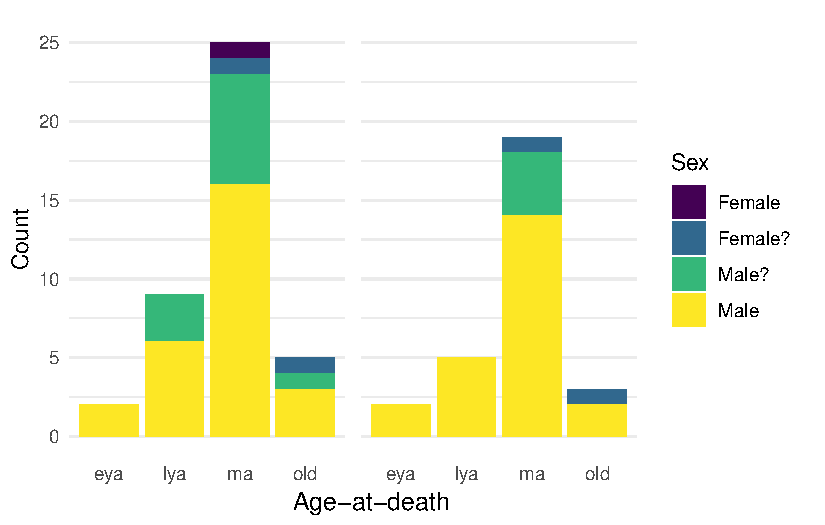
\includegraphics{05-article_files/figure-pdf/fig-sample-demography-1.pdf}

}

\caption{\label{fig-sample-demography}Overview of sample demography.
Left plot is the first batch and right plot is the replication batch
with 29 of the individuals from the first batch. eya = early young adult
(18-24 years); lya = late young adult (25-34 years); ma = middle adult
(35-49 years); old = old adult (50+ years). Male? = probable male;
Female? = probable female.}

\end{figure}%

\section{Methods}\label{methods}

\subsection{Skeletal analysis}\label{skeletal-analysis}

Demographic and pathological analyses were conducted in the Laboratory
for Human Osteoarchaeology at Leiden University. Sex was estimated using
cranial and pelvic morphological traits
(\citeproc{ref-Standards1994}{Buikstra \& Ubelaker, 1994}). Age-at-death
was estimated using dental wear, auricular and pubic surface appearance,
cranial suture closure, and epiphyseal fusion
(\citeproc{ref-SucheyBrooks1990}{Brooks \& Suchey, 1990};
\citeproc{ref-buckberryAuricular2002}{Buckberry \& Chamberlain, 2002};
\citeproc{ref-Standards1994}{Buikstra \& Ubelaker, 1994};
\citeproc{ref-lovejoyAuricular1985}{Lovejoy et al., 1985};
\citeproc{ref-meindlSutureClosure1985}{Meindl \& Lovejoy, 1985}), and
divided into the following categories: early young adult (18-24 years),
late young adult (25-34 years), middle adult (35-49 years), old adult
(50+ years). Preservation was visually scored on a four-stage scale
(excellent, good, fair, poor) based on the surface condition of the
bones and the extent of taphonomic degradation.

\subsubsection{Paleopathology}\label{paleopathology}

Pathological conditions and lesions that occur frequently in the
population were included in the analysis. Data were dichotomised to
presence/absence to allow for statistical analysis. Osteoarthritis was
considered present in cases where eburnation was visible on one or more
joint surfaces. Vertebral osteophytosis is identified by marginal
lipping and/or osteophyte formation on the margin of the superior and
inferior surfaces of the vertebral body. Cribra orbitalia was diagnosed
based on the presence of pitting on the superior surface of the orbit.
No distinction was made between active or healing lesions. Degenerative
disc disease, or spondylosis, is identified as a large diffuse
depression of the superior and/or inferior surfaces of the vertebral
body (\citeproc{ref-rogersPalaeopathologyJoint2000}{Rogers, 2000}).
Schmorl's nodes are identified as any cortical depressions on the
surface of the vertebral body. Data on chronic maxillary sinusitis from
Casna et al. (\citeproc{ref-casnaUrbanizationRespiratory2021}{2021})
were included in this study to assess the relationship between upper
respiratory diseases with environmental factors (i.e.~tobacco smoke,
caffeine consumption). Lesions associated with chronic maxillary
sinusitis as defined by Boocock et al.
(\citeproc{ref-boocockMaxillarySinusitis1995}{1995}) were recorded for
each individual and classified as ``pitting'', ``spicule-type bone
formation'', ``remodeled spicules'', or ``white pitted bone''. chronic
maxillary sinusitis was scored as absent when the sinus presented smooth
surfaces with little or no associated pitting.

\subsubsection{Dental pathology}\label{dental-pathology}

Caries ratios were calculated by dividing the number of lesions by the
number of teeth scored, resulting in a single caries ratio per
individual. If the surface where the lesion originated is not visible,
i.e.~if the lesion covered multiple surfaces, this was scored as
``crown''. Calculus indices were calculated according to Greene and
colleagues (\citeproc{ref-greeneQuantifyingCalculus2005}{2005}).
Calculus was scored with a four-stage scoring system (0-3) to score
absent, slight, moderate, and heavy calculus deposits
(\citeproc{ref-brothwellDiggingBones1981}{Brothwell, 1981}) on the
lingual, buccal (and labial), and interproximal surfaces of each tooth.
Only one score was used for the combined interproximal surfaces,
resulting in three scores per tooth (when surfaces are intact), and four
calculus indices per individual; upper anterior, upper posterior, lower
anterior, lower posterior. Each index was calculated by dividing the sum
of calculus scores for each surface by the total number of surfaces
scored in each quadrant. If a tooth could not be scored on all three
surfaces, the tooth was not included
(\citeproc{ref-greeneQuantifyingCalculus2005}{Greene et al., 2005}).
Periodontitis was scored on a visual four-stage (0-3) scoring system
according to distance from cemento-enamel junction of each tooth to
alveolar bone (\citeproc{ref-maatManualPhysical2005}{Maat \& Mastwijk,
2005}).

\subsection{Calculus sampling}\label{calculus-sampling}

Where possible, we used material that had already been sampled for a
previous study to prevent unnecessary repeated sampling of individuals.
Calculus from the previous study was sampled in a dedicated ancient DNA
laboratory at the Laboratories of Molecular Anthropology and Microbiome
Research in Norman, Oklahoma, U.S.A, using established ancient DNA
protocols. More details on the methods can be found in the published
articles (\citeproc{ref-ziesemer16SChallenges2015}{Ziesemer et al.,
2015}, \citeproc{ref-ziesemerGenomeCalculus2018}{2018}). Of the 41
individuals that were originally included in our sample, 29 were
replicated in a separate analysis only using calculus from the previous
study.\\
New dental calculus samples were taken under sterile conditions in a
positive pressure laminar flow hood in a dedicated dental calculus lab
at Leiden University. The surface of the tooth was lightly brushed with
a sterile, disposable toothbrush to get rid of surface contaminants. A
sterile dental curette was then used to scrape calculus from the tooth
onto weighing paper, which was transferred to 1.5 ml Eppendorf tubes.
All calculus samples were sent to the Department of Forensic Medicine at
Aarhus University for ultra-high-performance liquid
chromatography-tandem mass spectrometry (UHPLC-MS/MS) analysis.

\subsection{UHPLC-MS/MS}\label{uhplc-msms}

The list of targeted compounds included both naturally occurring
compounds known to have been used in the past, as well as synthetic
modern drugs that did not exist at the time (e.g.~Fentanyl, MDMA,
Amphetamine). These were part of the toxicology screening for the
original method (\citeproc{ref-sorensenDrugsCalculus2021}{Sørensen et
al., 2021}), developed on cadavers. In our study they serve as an
authentication step, as their presence in archaeological samples could
only be the result of contamination.

Briefly, samples of dental calculus were washed three times each with
one mL of methanol (MeOH), to remove surface contaminants. The wash
solutions were collected separately. The solvent was evaporated and the
residues were dissolved in 50 µL 30\% MeOH. The washed calculus was
homogenized in presence of 0.5 M citric acid using a lysing tube with
stainless steel beads. Following one hour of incubation the dissolution
extract was cleaned by weak and strong cation-exchange. After
evaporation of the elution solvent the residue was dissolved in 50 µL
30\% MeOH. The final extracts obtained from washing and dissolution of
the dental calculus were analysed by UHPLC-MS/MS using a reversed-phase
biphenyl column for chromatography. To obtain quantitative results,
isotope dilution was applied. For more details about the method and
validation, see the original study by Sørensen and colleagues
(\citeproc{ref-sorensenDrugsCalculus2021}{2021}).

\subsection{Statistical analysis}\label{statistical-analysis-1}

All compounds and pathological conditions/lesions were converted to a
presence/absence score. Pearson product-moment correlation was applied
to the dichotomised pathological lesions (point-biserial correlation),
compound concentrations, calculus indices, and caries ratios to explore
relationships paired continuous-continuous variables and paired
continuous-binary variables. Compound concentrations were then
dichotomised to presence/absence, and the caries ratio and calculus
index for each individual were converted to an ordinal score from 0 to 4
by using quartiles. Polychoric correlation was applied to the paired
dichotomous variables and dichotomous-ordinal variables.

All statistical analysis was conducted in R version 4.3.3 (2024-02-29),
Angel Food Cake, (\citeproc{ref-Rbase}{R Core Team, 2020}). Data
wrangling was conducted with the \textbf{tidyverse}
(\citeproc{ref-tidyverse2019}{Wickham et al., 2019}) and visualisations
were created using \textbf{ggplot2} (\citeproc{ref-ggplot2}{Wickham,
2016}). Polychoric correlations were calculated with the \textbf{psych}
package (\citeproc{ref-Rpsych}{Revelle, 2022}).

\section{Results}\label{results-2}

Multiple compounds were detected in the dental calculus samples.
Compounds detected at a lower concentration than the lower limit of
quantitation (LLOQ) were considered not present. Not all the compounds
detected in the first batch could be replicated in the second batch
(Table~\ref{tbl-compound-detect}). For a full list of targeted
compounds, see Supplementary Material.

\begin{longtable}[]{@{}lllr@{}}

\caption{\label{tbl-compound-detect}Target compound including whether it
was detected (TRUE) or not (FALSE) in each batch, as well as the lower
limit of quantitation (LLOQ) in ng. CBD = cannabidiol; CBN = cannabinol;
THC = tetrahydrocannabinol; THCA-A = tetrahydrocannabinolic acid A;
THCVA = tetrahydrocannabivarin acid.}

\tabularnewline

\toprule\noalign{}
Compound & Batch 1 & Batch 2 & LLOQ \\
\midrule\noalign{}
\endhead
\bottomrule\noalign{}
\endlastfoot
CBD & TRUE & FALSE & 0.050 \\
CBN & TRUE & FALSE & 0.050 \\
Caffeine & TRUE & TRUE & 0.050 \\
Cocaine & TRUE & FALSE & 0.025 \\
Cotinine & TRUE & TRUE & 0.050 \\
Nicotine & TRUE & TRUE & 0.100 \\
Salicylic acid & TRUE & TRUE & 0.500 \\
THC & TRUE & FALSE & 0.100 \\
THCA-A & TRUE & FALSE & 0.025 \\
THCVA & TRUE & FALSE & 0.010 \\
Theophylline & TRUE & TRUE & 0.010 \\

\end{longtable}

The pattern we expect to see in authentic compounds representing
compounds trapped within the dental calculus, is a reduction in the
quantity from wash 1 to wash 3 as potential surface contaminants are
washed off, and then a spike in the final extraction when entrapped
compounds are released and detected.

Most plots show a large increase in extracted mass of a compound between
the calculus wash extracts (wash 1-3) and the dissolved calculus (calc).
Most samples containing theophylline and caffeine had the largest
quantity of the compound extracted from the first wash, then decreasing
in washes 2 and 3. There is an increase between wash 3 and the dissolved
calculus in all samples. The patterns are consistent across batches 1
and 2. Nicotine and cotinine have the same relative quantities in the
samples, i.e., the sample with the highest extracted quantity of
nicotine also had the highest extracted quantity of cotinine
(Figure~\ref{fig-auth-plot-batch2}).

\begin{figure}

\centering{

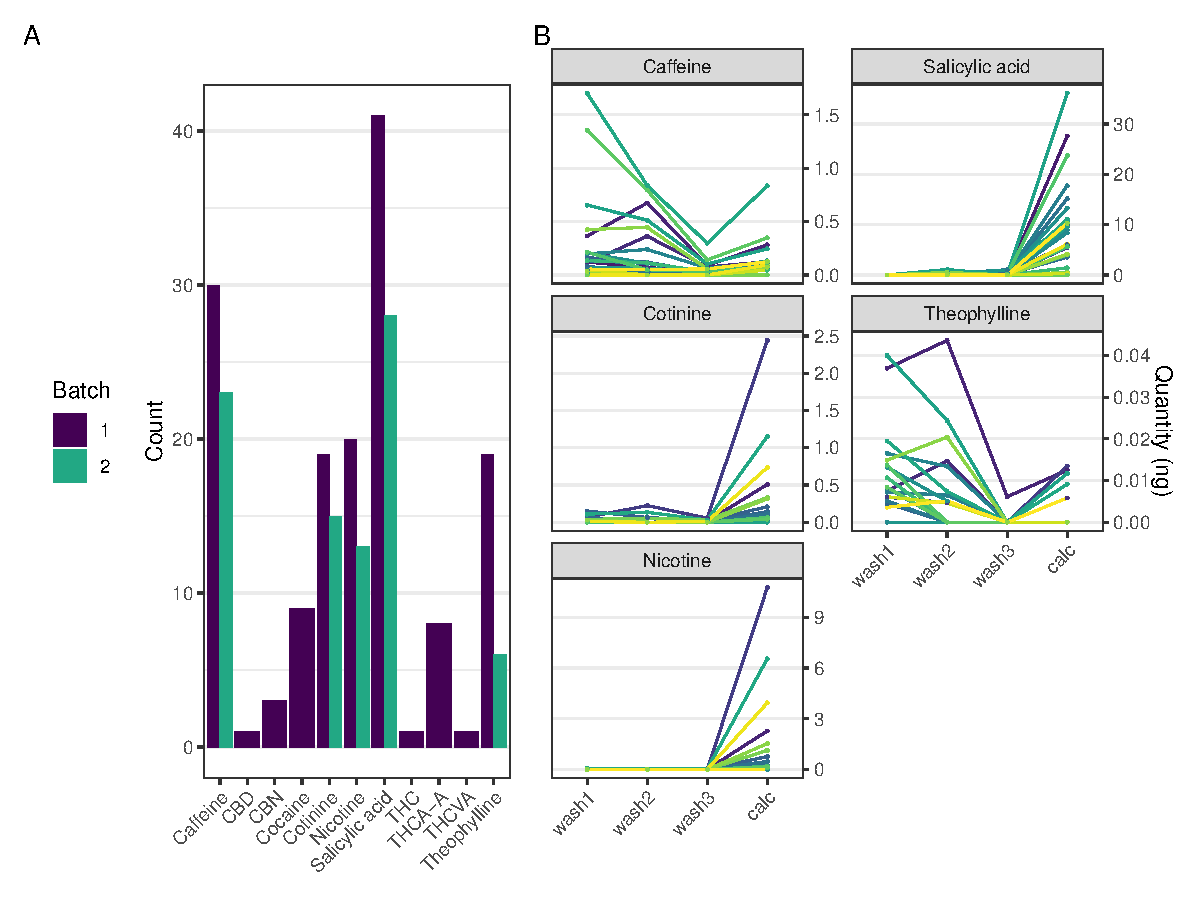
\includegraphics{05-article_files/figure-pdf/fig-auth-plot-batch2-1.pdf}

}

\caption{\label{fig-auth-plot-batch2}(A) Number of samples in which each
compound was detected in the first and second batch. (B) Quantity (ng)
of each compound extracted from each sample in batch 2. The plot
displays the extracted quantity across the three washes and final
calculus extraction (calc). Each coloured line represents a different
calculus sample. CBD = cannabidiol; CBN = cannabinol; THC =
tetrahydrocannabinol; THCA-A = tetrahydrocannabinolic acid A; THCVA =
tetrahydrocannabivarin acid.}

\end{figure}%

To see if preservation of the skeletal remains had any effect on the
detection of compounds, we compare extracted quantities of compounds to
the various levels of skeletal preservation. Our results from batch 2
suggest that detection of a compound may be linked to the preservation
of the skeleton, with better preservation leading to increased
extraction quantity (Figure~\ref{fig-detection-preservation}A). We also
find a weak positive correlation between the weight of the calculus
sample and the quantity of compound extracted from the calculus
(Figure~\ref{fig-detection-preservation}B).

\begin{figure}

\centering{

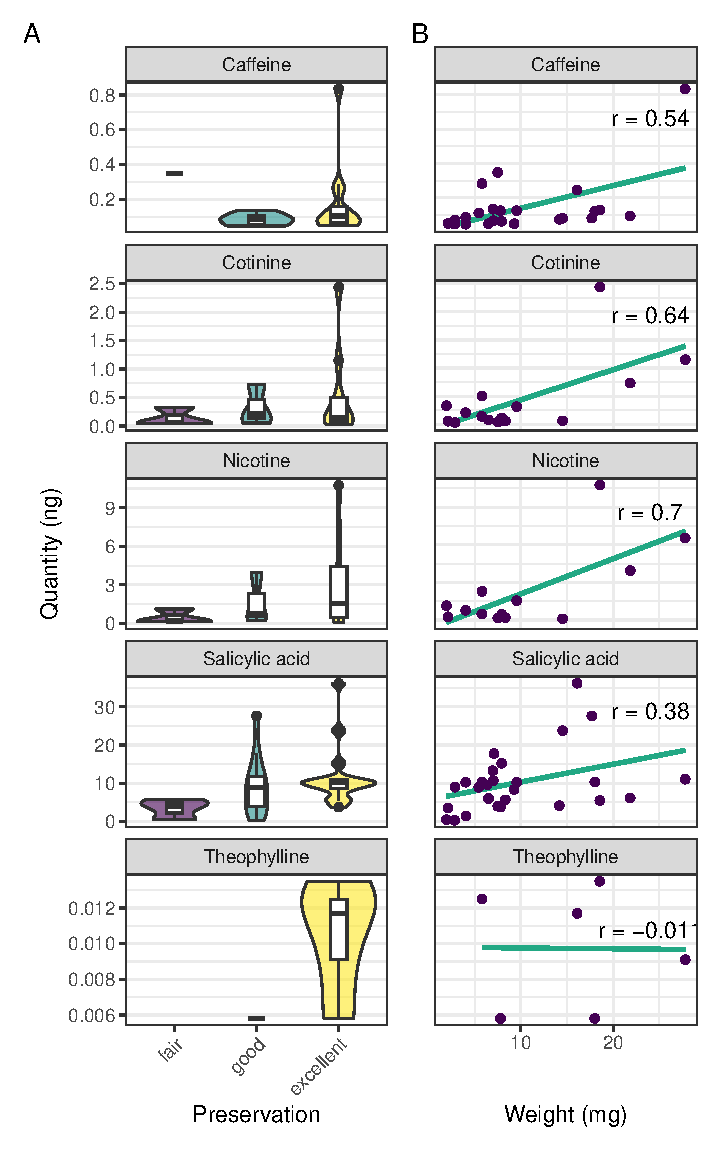
\includegraphics{05-article_files/figure-pdf/fig-detection-preservation-1.pdf}

}

\caption{\label{fig-detection-preservation}(A) Violin plot with overlaid
box plots depicting the distribution of extracted quantities of each
compound from batch 2 separated by state of preservation of the
skeleton. (B) Extracted quantity (ng) of compound plotted against
weights of the calculus samples from batch 2. r = Pearson correlation
coefficient.}

\end{figure}%

The presence of pipe notch(es) in an individual and concurrent detection
of nicotine and/or cotinine is used as a crude indicator of the accuracy
of the method. Only males were used in accuracy calculations, as pipe
notches are ubiquitous in males, but not in females. In batch 2, the
method was able to detect some form of tobacco in 14 of 25 individuals
with a pipe notch (56.0\%). When also considering correct the absence of
a tobacco alkaloid together with the absence of a pipe notch, the
accuracy of the method is 59.3\%. Accuracy in the old adult age category
is 100.0\%, but with only 2 individuals.

One individual---an old adult, probable female---was positive for both
nicotine and cotinine, and had no signs of a pipe notch.

\subsection{Correlations between detected alkaloids and
diseases}\label{correlations-between-detected-alkaloids-and-diseases}

For further statistical analyses, only the UHPLC-MS/MS results from
batch 2 were used, as batch 1 had multiple compounds that were not
detected in batch 2 and may have been contaminated.

\begin{longtable}[]{@{}
  >{\raggedright\arraybackslash}p{(\columnwidth - 16\tabcolsep) * \real{0.1500}}
  >{\raggedright\arraybackslash}p{(\columnwidth - 16\tabcolsep) * \real{0.1000}}
  >{\raggedright\arraybackslash}p{(\columnwidth - 16\tabcolsep) * \real{0.1000}}
  >{\raggedright\arraybackslash}p{(\columnwidth - 16\tabcolsep) * \real{0.1000}}
  >{\raggedright\arraybackslash}p{(\columnwidth - 16\tabcolsep) * \real{0.1000}}
  >{\raggedright\arraybackslash}p{(\columnwidth - 16\tabcolsep) * \real{0.1000}}
  >{\raggedright\arraybackslash}p{(\columnwidth - 16\tabcolsep) * \real{0.1500}}
  >{\raggedright\arraybackslash}p{(\columnwidth - 16\tabcolsep) * \real{0.1000}}
  >{\raggedright\arraybackslash}p{(\columnwidth - 16\tabcolsep) * \real{0.1000}}@{}}

\caption{\label{tbl-pearson}Pearson correlation (\emph{r}) on
dichotomous skeletal lesions and compound concentrations (ng/mg) from
the second batch. Correlations between pairs of dichotomous variables
are removed due to incompatibility with a Pearson correlation. Moderate
and strong correlations in \textbf{bold}. OA = osteoarthritis; VOP =
vertebral osteophytosis; SN = Schmorl's nodes; DDD = degenerative disc
disease; CO = cribra orbitalia; CMS = chronic maxillary sinusitis; SA =
salicylic acid; PN = pipe notches.}

\tabularnewline

\toprule\noalign{}
\begin{minipage}[b]{\linewidth}\raggedright
\end{minipage} & \begin{minipage}[b]{\linewidth}\raggedright
Caries
\end{minipage} & \begin{minipage}[b]{\linewidth}\raggedright
Nicotine
\end{minipage} & \begin{minipage}[b]{\linewidth}\raggedright
SA
\end{minipage} & \begin{minipage}[b]{\linewidth}\raggedright
Calculus
\end{minipage} & \begin{minipage}[b]{\linewidth}\raggedright
PN
\end{minipage} & \begin{minipage}[b]{\linewidth}\raggedright
Theophylline
\end{minipage} & \begin{minipage}[b]{\linewidth}\raggedright
Caffeine
\end{minipage} & \begin{minipage}[b]{\linewidth}\raggedright
Cotinine
\end{minipage} \\
\midrule\noalign{}
\endhead
\bottomrule\noalign{}
\endlastfoot
OA & -0.12 & -0.07 & 0.21 & 0.07 & 0.14 & 0.28 & 0 & -0.07 \\
VOP & -0.09 & -0.16 & 0.34 & 0.06 & 0.25 & -0.06 & 0.01 & -0.13 \\
SN & -0.24 & 0.16 & 0.09 & 0.09 & 0.17 & 0.24 & 0.16 & 0.09 \\
DDD & 0 & 0 & 0.19 & -0.39 & -0.08 & 0.31 & 0.06 & -0.01 \\
CO & 0.06 & -0.05 & 0.2 & 0.14 & -0.2 & -0.11 & 0.19 & -0.06 \\
CMS & -0.19 & 0.28 & 0 & -0.27 & 0.03 & 0.19 & 0.36 & 0.22 \\
Caries & & -0.2 & -0.36 & -0.15 & -0.17 & -0.21 & 0 & -0.22 \\
Nicotine & & & -0.21 & 0.01 & -0.01 & \textbf{0.43} & 0.14 &
\textbf{0.98} \\
SA & & & & 0.14 & 0.37 & 0.04 & 0.17 & -0.17 \\
Calculus & & & & & 0.13 & -0.15 & -0.13 & 0.03 \\
PN & & & & & & -0.16 & 0.18 & -0.01 \\
Theophylline & & & & & & & \textbf{0.51} & 0.36 \\
Caffeine & & & & & & & & 0.08 \\

\end{longtable}

Point-biserial correlation was conducted on paired continuous and
dichotomous variables, to see if any relationships exist between
extracted concentrations and other variables. The strongest
point-biserial (Pearson) correlation correlations were a near-perfect
positive correlation between cotinine and nicotine (0.98), and moderate
correlations between theophylline and nicotine (0.43), caffeine and
theophylline (0.51) (Table~\ref{tbl-pearson}).

Polychoric correlation was conducted on the dichotomised compounds and
pathological conditions, as well as the discretised dental diseases.
Salicylic acid was removed due to its ubiquitous presence in the sample,
and is likely to cause spurious correlations. Strong correlations were
found between cotinine and nicotine (0.85). Moderate correlations were
found between OA and DDD (0.47), VOP and periodontitis (0.49), SN and
cotinine (0.56), DDD and calculus (-0.42), CMS and caffeine (0.53),
caries and periodontitis (0.52), periodontitis and VOP (0.49),
periodontitis and age-at-death (0.41), nicotine and SN (0.53), calculus
and DDD (-0.42), age-at-death and theophylline (-0.45), theophylline and
age-at-death (-0.45), caffeine and periodontitis (0.49), cotinine and
CMS (0.43). Remaining correlations were weak or absent
(Figure~\ref{fig-polycorr}). Correlations with age will be depressed
because age was largely controlled for in the sample selection.

\begin{figure}

\centering{

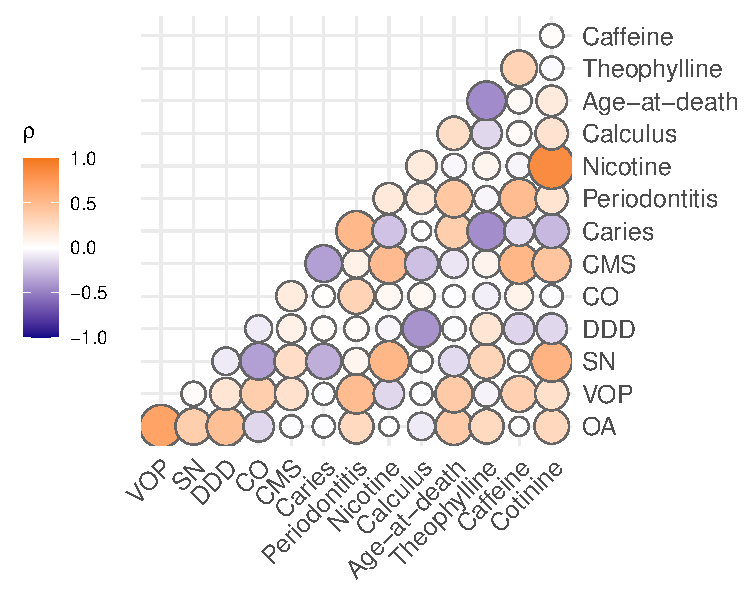
\includegraphics{05-article_files/figure-pdf/fig-polycorr-1.pdf}

}

\caption{\label{fig-polycorr}Plot of the polychoric correlations
(\emph{rho}). Larger circles and increased opacity indicates a stronger
correlation coefficient. OA = osteoarthritis; VOP = vertebral
osteophytosis; SN = Schmorl's nodes; DDD = degenerative disc disease; CO
= cribra orbitalia; CMS = chronic maxillary sinusitis; SA = salicylic
acid.}

\end{figure}%

\section{Discussion}\label{discussion-2}

In this study we were able to extract and identify multiple alkaloids
and salicylic acid from the dental calculus of individuals from
Middenbeemster, a 19th century Dutch archaeological site. We applied
ultra-high-performance liquid chromatography-tandem mass spectrometry
(UHPLC-MS/MS) using a method that was validated by co-occurrence of
drugs and metabolites in dental calculus and blood
(\citeproc{ref-sorensenDrugsCalculus2021}{Sørensen et al., 2021}). Here
we have shown that the method can also be successfully applied to
archaeological dental calculus. We extend findings from previous studies
on alkaloids in archaeological samples by detecting multiple different
alkaloids in dental calculus, including nicotine, cotinine, caffeine,
theophylline, and salicylic acid. The detection of these compounds was
solidified in a replication analysis on different samples from the same
individuals. Cocaine and multiple cannabinoids were also detected during
the first analysis, but were not replicated. We contextualize these
findings within the historical and archaeological evidence for
consumption of these drugs and dietary compounds.

Nicotine and its principal/main metabolite, cotinine, were strongly
positively correlated, both in concentration and presence/absence in
individuals (Table~\ref{tbl-pearson} and Figure~\ref{fig-polycorr}). The
detection of nicotine and cotinine is not surprising, as pipe-smoking in
the Beemsterpolder is well-documented in the literature
(\citeproc{ref-aten400Jaar2012}{Aten et al., 2012};
\citeproc{ref-boumanBegravenis2017}{Bouman, 2017}), and visible on the
skeletal remains as pipe notches
(\citeproc{ref-lemmersMiddenbeemster2013}{Lemmers et al., 2013}). There
is also documented medicinal use of nicotine in the Beemsterpolder,
where a tobacco-smoke enema was used for headaches, respiratory
problems, colds, and drowsiness from around 1780 to 1830
(\citeproc{ref-aten400Jaar2012}{Aten et al., 2012}). In our sample, we
also detected nicotine and cotinine (replicated) in an old adult,
probable female individual. In this particular case it is unlikely that
the compounds entered the dental calculus through pipe-smoking, as the
individual had no visible pipe notches; more likely the tobacco entered
through an alternate mode of consumption, secondhand smoke, or the
aforementioned tobacco-smoke enema.

Theophylline and caffeine were positively correlated in our samples,
though to a lesser extent than nicotine and cotinine, so we are unable
to determine if they originated from the same source
(Table~\ref{tbl-pearson} and Figure~\ref{fig-polycorr}). Caffeine and
theophylline have very similar chemical structures, so we expect they
would experience similar rates of incorporation and degradation,
allowing us to interpret the ratio and correlations between the
compounds. Caffeine is present in coffee, tea, and cocoa beans, with
concentrations slightly higher in coffee
(\citeproc{ref-bispoSimultaneousDetermination2002}{Bispo et al., 2002};
\citeproc{ref-chinCaffeineContent2008}{Chin et al., 2008};
\citeproc{ref-srdjenovicSimultaneousHPLC2008}{Srdjenovic et al., 2008};
\citeproc{ref-stavricVariabilityCaffeine1988}{Stavric et al., 1988}).
Theophylline is present in both coffee beans and tea leaves, but in
negligible quantities
(\citeproc{ref-stavricVariabilityCaffeine1988}{Stavric et al., 1988}).
It is also a primary metabolite of caffeine produced by the liver. Given
the low correlation, there are likely multiple sources of caffeine and
theophylline in the population, with tea and coffee being the most
obvious.\\
Tea consumption had become widespread in the Netherlands by 1820,
reaching all parts of society
(\citeproc{ref-nierstraszTeaTrade2015}{Nierstrasz, 2015, p. 91}).
Historically, we also know that both tea and coffee were consumed in the
Beemsterpolder during the 19th century. `Theegasten' (teatime) was a
special occasion occurring from 15.00-20.00 hours, where tea was served
along with the evening bread
(\citeproc{ref-schuijtemakerTeTheegasten2011}{Schuijtemaker, 2011}).
Many households also owned at least one coffee pot and tea pot
(\citeproc{ref-boumanBegravenis2017}{Bouman, 2017}). Distinguishing
between tea, coffee, and chocolate may be possible by also including
theobromine and comparing ratios of the compounds, as theobromine is
present in higher quantities in chocolate compared to caffeine and
theophylline (\citeproc{ref-alanonAssessmentFlavanol2016}{Alañón et al.,
2016}; \citeproc{ref-bispoSimultaneousDetermination2002}{Bispo et al.,
2002}; \citeproc{ref-stavricVariabilityCaffeine1988}{Stavric et al.,
1988}). However, In addition to oral factors affecting alkaloid uptake
in dental calculus, there is some indication that theobromine does not
preserve well in the archaeological record
(\citeproc{ref-velskoDentalCalculus2017}{Velsko et al., 2017}), and
frequent consumption of all three items would be difficult to parse.
Additionally, we do not understand well enough the effect of the burial
on these specific compounds, and the original concentration of the
compounds in plants can be quite variable
(\citeproc{ref-kingCautionaryTales2017}{King et al., 2017}).

Salicylic acid was found in all but one individual in our sample. It can
be extracted from the bark of willow trees, \emph{Salix alba}, and has
long been used for its pain-relieving properties
(\citeproc{ref-bruinsmaBijdragenTot1872}{Bruinsma, 1872, p. 119}). It is
also present in many plant-based foods
(\citeproc{ref-duthieNaturalSalicylates2011}{Duthie \& Wood, 2011};
\citeproc{ref-malakarNaturallyOccurring2017}{Malakar et al., 2017}),
including potatoes, which were a staple of the Beemsterpolder diet
(\citeproc{ref-aten400Jaar2012}{Aten et al., 2012}). The extracted
quantity from our samples decreased over the three washes, followed by a
sharp increase in the final calculus extraction, which is what we would
expect to see if the salicylic acid was incorporated during life
(Figure~\ref{fig-auth-plot-batch2}). It is important to note that,
especially with salicylic acid, there is a possibility for the compound
to enter the calculus through contact with the surrounding soil.
Salicylic acid is a very mobile organic acid
(\citeproc{ref-badriRegulationFunction2009}{Badri \& Vivanco, 2009};
\citeproc{ref-chenCa2Dependent2001}{Chen et al., 2001}) and the
ubiqutous presence in our samples may be explained by the compound
leching into the dental calculus from the burial environment. We can
therefore not confidently rule out environmental contamination without
analysing samples from the surrounding soil.

Cannabinoids---specifically THC, THCA-A, THCVA, CBD, CBN---were found in
the first batch, but none were replicated in the second batch. Medicinal
use of cannabinoids has been well-established in Europe since
Medieval-times, and it was also grown in the Netherlands
(\citeproc{ref-bruinsmaBijdragenTot1872}{Bruinsma, 1872}).
Administration was most common in the form of concoctions containing
various portions of the cannabis plant for ingestion; not until the late
19th century did it become recommended to smoke it for more immediate
effects (\citeproc{ref-clarkeCannabisEvolution2013}{Clarke, 2013}).
Dutch medicinal preparations were used to treat a variety of ailments
and symptoms, including pain, inflammation, various stomach ailments,
gout, and joint pains
(\citeproc{ref-clarkeCannabisEvolution2013}{Clarke, 2013}). Because
cannabinoids have an affinity for protein-binding, they are less likely
to diffuse from serum to saliva
(\citeproc{ref-coneInterpretationOral2007}{Cone \& Huestis, 2007}). This
may make them difficult to detect in dental calculus unless the
cannibinoids were consumed orally; even then, the overall instability of
some cannabinoids could also limit detection
(\citeproc{ref-lindholstLongTerm2010}{Lindholst, 2010};
\citeproc{ref-sorensenEffectAntioxidants2018}{Sørensen \& Hasselstrøm,
2018}). Given the lack of replication, we cannot with security confirm
that cannabis was used by the Beemster population.

Despite many of our sampled individuals having lived during the height
of the opium era in the Netherlands
(\citeproc{ref-machtHistoryOpium1915}{Macht, 1915}), none of the
targeted opioids (morphine, codeine, thebaine, papaverine, norcodeine,
noscapine) were detected. The absence of opioids could be a result of
the people ascribing more to the ``traditional'' rather than
``scientific'' medicine, although laudanum and another opium containing
concoction was part of the ``traditional'' medicine in the Netherlands
(\citeproc{ref-leuwProhibitionLegalization1994}{Leuw \& Marshall,
1994}), including Middenbeemster (\citeproc{ref-aten400Jaar2012}{Aten et
al., 2012}). It was also generally considered a drug of the upper class
(\citeproc{ref-scheltemaOpiumTrade1907}{Scheltema, 1907}), and may have
been more common in urban centers. The absence could also be attributed
to postmortem degradation. It has been shown that, while morphine is
abundant in opium, it degrades rapidly. Thebaine and papaverine are more
resistant to various ageing processes
(\citeproc{ref-chovanecOpiumMasses2012}{Chovanec et al., 2012}),
however, these were also absent from our samples.

The only strictly modern compound (at least in a European context)
detected in the sample was cocaine, which was detected in the first
batch of samples. Our sample is derived from an early--mid 19th century
population, and cocaine was isolated in 1860 by Albert Niemann, and
entered popular medical practice in 1884. Coca arrived in Europe as
early as 1771, but as botanical specimens rather than for consumption,
and there were also issues importing enough viable specimens of coca for
cocaine extraction (\citeproc{ref-abucaCocaTrade2019}{Abduca, 2019, p.
108}; \citeproc{ref-mortimerHistoryCoca1901}{Mortimer, 1901, p. 179}).
This would have been the first case of coca-leaf-consumption in Europe;
however, we were unable to replicate any of the cocaine results in the
second batch. We suspect that the original detection of cocaine was a
result of lab contamination during analysis.

We explored the relationship between detected compounds and various
skeletal indicators, such as pathological and dental lesions,
preservation, and pipe notches. We found some evidence to suggest that
preservation of the skeleton influences the recovery of compounds from
the dental calculus, with well-preserved skeletons potentially serving
as a better target for sampling.\\
We found a positive correlation between CMS and nicotine, which may be
indicative of the impact tobacco smoking had on the respiratory health
of the Beemster inhabitants. Tobacco smoke may play a significant role
in diseases of the upper respiratory tract, including chronic maxillary
sinusitis (\citeproc{ref-rehImpactTobacco2012}{Reh et al., 2012}).
Although the mechanisms by which smoking increases the risk of
infections is not fully understood, solid evidence has been presented
linking tobacco smoke to increased mucosal permeability and impairment
of mucociliary clearance
(\citeproc{ref-arcaviCigaretteSmoking2004}{Arcavi \& Benowitz, 2004}).
Such changes, together with an altered immunologic response, are thought
to predispose to the development of chronic maxillary sinusitis
(\citeproc{ref-slavinDiagnosisManagement2005}{Slavin et al., 2005}).\\
We also observed a moderate positive correlation between chronic
maxillary sinusitis and caffeine which contradicts previous research
linking chronic coffee consumption with a positive effect on the
respiratory system, suggesting a preventive association between caffeine
intake and pneumonia (e.g. \citeproc{ref-alfaroChronicCoffee2018}{Alfaro
et al., 2018}; \citeproc{ref-kondoAssociationCoffee2021}{Kondo et al.,
2021}). However, while the lower respiratory tract seems to benefit from
chronic coffee consumption, it is possible that elevated caffeine intake
impacts mucosal moisture due to its dehydrating effect
(\citeproc{ref-maughanCaffeineIngestion2003}{Maughan \& Griffin, 2003}),
thereby exposing individuals to greater risk of sinus infection.

The detection of nicotine in dental calculus has previously been
presented by Eerkens and colleagues
(\citeproc{ref-eerkensDentalCalculus2018}{2018}) in two individuals from
pre-contact California. They also targeted caffeine, cotinine, and
theophylline in their samples, but were unable to detect any of them. It
remains to be seen whether this is due to differences in methods used,
or due to our samples being more recent. They also suggest that the
choice of tooth for sampling may impact the detection of certain
compounds, as the incorporation in dental calculus may depend on the
mode of consumption. Tobacco smokers may have more nicotine present in
calculus on incisors, whereas tobacco chewers may have more on molars
(\citeproc{ref-eerkensDentalCalculus2018}{Eerkens et al., 2018}).
However, sampling may not be limited to mode of consumption. The
presence of cotinine suggests that the excretion of a compound after
being metabolised in the body is also a source of deposition, and that
deposition of alkaloids in dental calculus can occur both on the way
into the body, i.e.~during consumption, and on the way out,
i.e.~disposal of waste products via saliva secretion into the mouth.
Especially mucin-rich saliva from the sublingual and submandibular
glands preferentially binds toxins
(\citeproc{ref-doddsHealthBenefits2005}{Dodds et al., 2005}), and since
these glands are located closest to the lower incisors, they may be the
most effective target for these studies. This has yet to be
systematically tested in archaeological dental calculus. Because we
homogenised samples from multiple teeth of an individual, we were unable
to test the effect of oral biogeography. It is also possible that
resident microflora within biofilms contribute to alkaloid breakdown and
that the presence of caffeine and nicotine metabolites following direct
ingestion can be explained by this pathway. However, the literature on
biofilm biodegradation of alkaloids is limited, and \emph{in vitro}
studies have only found minimal contributions by certain oral bacteria
in isolation (\citeproc{ref-cogoVitroEvaluation2008}{Cogo et al., 2008};
\citeproc{ref-sunMetabolomicsEvaluation2016}{Sun et al., 2016}); it is
possible that a larger role is played by oral bacteria within larger,
more metabolically active communities, e.g.~biofilms
(\citeproc{ref-takahashiOralMicrobiome2015}{Takahashi, 2015}).

Targeting individuals with moderate-to-large calculus deposits likely
biased our sample, as the presence of calculus may increase the risk of
premature death (\citeproc{ref-yaussyCalculusSurvivorship2019}{Yaussy \&
DeWitte, 2019}). Additionally, periodontal disease (often linked to the
presence of calculus) is a risk-factor for respiratory diseases, if
periodontal and respiratory pathogens enter the bloodstream
(\citeproc{ref-azarpazhoohSystematicReview2006}{Azarpazhooh \& Leake,
2006}; \citeproc{ref-scannapiecoRoleOral1999}{Scannapieco, 1999};
\citeproc{ref-scannapiecoPotentialAssociations2001}{Scannapieco \& Ho,
2001}). In our sample, the percentage of chronic maxillary sinusitis
(37.0\%) is lower than in another (more representative) male sample
(44.1\%) (\citeproc{ref-casnaUrbanizationRespiratory2021}{Casna et al.,
2021}), and the caries percentage is similarly lower in our sample
(17.6\%) than a more representative sample (22.9\%)
(\citeproc{ref-lemmersMiddenbeemster2013}{Lemmers et al., 2013}).\\
We used the presence/absence of a pipe notch and concurrent detection of
tobacco as a crude estimate of the accuracy of the method, which we
found to be around 59.3\%. This is a very rough estimate, as the
presence of a pipe notch is likely not a perfect indicator of whether or
not someone consumed tobacco. Dental calculus is also more transient
than for example bone, as it can become dislodged during life,
intentionally or unintentionally, eliminating all trace of the alkaloids
consumed prior to its removal.\\
Following burial, compound stability over time will play a large role,
as will microbial degradation of compounds by bacteria and fungi in soil
(\citeproc{ref-liuNicotinedegradingMicroorganisms2015}{Liu et al.,
2015}), as well as the soil environment, such as temperature, pH, and
oxygen availability (\citeproc{ref-lindholstLongTerm2010}{Lindholst,
2010}; \citeproc{ref-mackiePreservationMetaproteome2017}{Mackie et al.,
2017}).\\
Due to this, quantitation of the detected compounds may have limited
value in archaeological samples due to degradation, and will greatly
affect our correlations related to concentration. The detected quantity
of a compound will also depend on the quantity in dental calculus during
life, which is largely controlled by the quantity consumed, how often
the calculus was disrupted/removed, metabolic breakdown of the compound,
and inter- and intra-individual factors related to stages of biofilm
maturation (\citeproc{ref-lustmannScanningElectron1976}{Lustmann et al.,
1976}; \citeproc{ref-velskoMicrobialDifferences2019}{Velsko et al.,
2019}; \citeproc{ref-zijngeBiofilmArchitecture2010}{Zijnge et al.,
2010}). In short, this means it is not really possible to equate the
absence of a compound as evidence for the absence of consumption, which
complicates the interpretation of our results. We have attempted to
minimise errors occurring due to this limitation by including a
relatively large sample of individuals and replicating our analysis.
Although, given the relatively low detection rate seen in tobacco, this
remains a major limitation, and will likely be compounded by increasing
antiquity of the samples.

Future studies should explore how sampling from various types of teeth
and their position in the mouth affects the probability of a compound
becoming entrapped in dental calculus. This may also be related to
properties within the oral cavity, as well as chemical properties of the
compounds, which facilitate or reduce the incorporation-potential, and
which incorporation pathways are more likely for a given compound.\\
We only targeted drugs that were included in the forensic toxicological
screenings, and therefore only covered a limited number of the potential
compounds that could be of interest for exploring past diets and
medicinal treatments. The list of targeted compounds can be expanded as
we discover more potential targets based on which specific
compounds/metabolites are more likely to be incorporated and preserved
in dental calculus.\\
There is an increasing interest in using oral fluid as a means of
detecting alkaloids in living individuals due to the non-invasive nature
of the testing compared to blood and urine sampling
(\citeproc{ref-coneSalivaTesting1993}{Cone, 1993};
\citeproc{ref-valenDetermination212017}{Valen et al., 2017}). These
\emph{in vivo} studies are a valuable source of method validation and
can help determine the feasibility of detecting certain alkaloids in
oral fluid and, subsequently, dental calculus. Archaeologists, though,
will likely be responsible for exploring dental-calculus-specific
incorporation and retention of alkaloids, as well as their long-term
preservation in the burial environment. Finally, following our
experience with salicylic acid, we encourage all future studies to
ensure that a control sample is taken from the soil, either from the
soil surrounding the individual, or, ideally, directly from the skeletal
remains. This should preferably happen before cleaning, but there will
often be soil left over in cavities (e.g.~nasal cavity, orbit, auditory
meatus).

While a major limitation is the uncertainty surrounding whether or not a
compound is actually absent, the power of the method lies in the ability
to detect dietary and other compounds that were incorporated via
multiple consumption pathways that are not detected by other methods.
Taking tobacco consumption as an example; while pipe notches are a
useful way to identify tobacco consumption, pipe smoking was not the
only mode of tobacco consumption, with others including chewing,
drinking, cigars, and snuff
(\citeproc{ref-goodmanTobaccoHistory1994}{Goodman, 1994, p. 67}).
Pipe-smoking was mainly practised by males
(\citeproc{ref-eerkensDentalCalculus2018}{Eerkens et al., 2018};
\citeproc{ref-lemmersMiddenbeemster2013}{Lemmers et al., 2013}), so
methods like the one presented here are suitable for exploring tobacco
consumption in an entire society, rather than a trivial subset of past
populations. Combined with other methods, it can also give us a more
complete picture of dietary patterns and medicinal/recreational
plant-use in the past by capturing multiple possible incorporation
pathways of dietary (and other) compounds.

\section{Conclusion}\label{conclusion-1}

This preliminary study outlines the benefits of using calculus to target
a variety of compounds that could have been consumed as medicine or
diet. This method allows us to directly address specific individuals,
which can be especially useful in individuals that are not always
well-documented in historic documentation, such as rural communities,
children and women. We also show that there are many limitations that
will need to be addressed going forward with this type of analysis, and
stress the need for more systematic research on the consumption of
alkaloid-containing items and their subsequent concentration and
preservation in dental calculus, in addition to how mode of consumption
may affect concentrations on different parts of the dentition. Another
limitation of dental calculus as a medium is the inter- and
intra-individual variability of its formation and the many factors that
can influence incorporation and retention of molecules and particles;
however, in the absence of hair and serum (quite uncommon in
archaeology), dental calculus represents an impressive long-term
reservoir of information regarding the consumption of various alkaloids,
whether dietary, medicinal, recreational, or otherwise.

\section*{References cited}\label{references-cited-4}
\addcontentsline{toc}{section}{References cited}

\markright{References cited}

\phantomsection\label{refs-5}
\begin{CSLReferences}{1}{0}
\bibitem[\citeproctext]{ref-abucaCocaTrade2019}
Abduca, R. (2019). Coca leaf transfers to {Europe}. {Effects} on the
consumption of coca in {North-western Argentina}. In M. Kaller \& F.
Jacob (Eds.), \emph{Transatlantic {Trade} and {Global Cultural Transfers
Since} 1492: {More} than {Commodities}}. {Routledge}.

\bibitem[\citeproctext]{ref-alanonAssessmentFlavanol2016}
Alañón, M. E., Castle, S. M., Siswanto, P. J., Cifuentes-Gómez, T., \&
Spencer, J. P. E. (2016). Assessment of flavanol stereoisomers and
caffeine and theobromine content in commercial chocolates. \emph{Food
Chemistry}, \emph{208}, 177--184.
\url{https://doi.org/10.1016/j.foodchem.2016.03.116}

\bibitem[\citeproctext]{ref-alfaroChronicCoffee2018}
Alfaro, T. M., Monteiro, R. A., Cunha, R. A., \& Cordeiro, C. R. (2018).
Chronic coffee consumption and respiratory disease: {A} systematic
review. \emph{The Clinical Respiratory Journal}, \emph{12}(3),
1283--1294. \url{https://doi.org/10.1111/crj.12662}

\bibitem[\citeproctext]{ref-arcaviCigaretteSmoking2004}
Arcavi, L., \& Benowitz, N. L. (2004). Cigarette {Smoking} and
{Infection}. \emph{Archives of Internal Medicine}, \emph{164}(20),
2206--2216. \url{https://doi.org/10.1001/archinte.164.20.2206}

\bibitem[\citeproctext]{ref-aten400Jaar2012}
Aten, D., Bossaers, K. W. J. M., \& Misset, C. (2012). \emph{{400 jaar
Beemster: 1612-2012}}. {Stichting Uitgeverij Noord-Holland}.

\bibitem[\citeproctext]{ref-azarpazhoohSystematicReview2006}
Azarpazhooh, A., \& Leake, J. L. (2006). Systematic {Review} of the
{Association Between Respiratory Diseases} and {Oral Health}.
\emph{Journal of Periodontology}, \emph{77}(9), 1465--1482.
\url{https://doi.org/10.1902/jop.2006.060010}

\bibitem[\citeproctext]{ref-badriRegulationFunction2009}
Badri, D. V., \& Vivanco, J. M. (2009). Regulation and function of root
exudates. \emph{Plant, Cell \& Environment}, \emph{32}(6), 666--681.
\url{https://doi.org/10.1111/j.1365-3040.2009.01926.x}

\bibitem[\citeproctext]{ref-bispoSimultaneousDetermination2002}
Bispo, M. S., Veloso, M. C. C., Pinheiro, H. L. C., De Oliveira, R. F.
S., Reis, J. O. N., \& De Andrade, J. B. (2002). Simultaneous
{Determination} of {Caffeine}, {Theobromine}, and {Theophylline} by
{High-Performance Liquid Chromatography}. \emph{Journal of
Chromatographic Science}, \emph{40}(1), 45--48.
\url{https://doi.org/10.1093/chromsci/40.1.45}

\bibitem[\citeproctext]{ref-boocockMaxillarySinusitis1995}
Boocock, P., Roberts, C. A., \& Manchester, K. (1995). Maxillary
sinusitis in {Medieval Chichester}, {England}. \emph{American Journal of
Physical Anthropology}, \emph{98}(4), 483--495.
\url{https://doi.org/10.1002/ajpa.1330980408}

\bibitem[\citeproctext]{ref-boumanBegravenis2017}
Bouman, J. (2017). {De Begravenis}. \emph{De Nieuwe Schouwschuit},
\emph{15}, 11--15.

\bibitem[\citeproctext]{ref-SucheyBrooks1990}
Brooks, S., \& Suchey, J. M. (1990). Skeletal age determination based on
the os pubis: {A} comparison of the {Acsádi-Nemeskéri} and
{Suchey-Brooks} methods. \emph{Human Evolution}, \emph{5}(3), 227--238.
\url{https://doi.org/10.1007/BF02437238}

\bibitem[\citeproctext]{ref-brothwellDiggingBones1981}
Brothwell, D. (1981). \emph{Digging up {Bones}: {The} excavation,
treatment and study of human skeletal remains} (3rd ed.). {British
Museum (Natural History)}.

\bibitem[\citeproctext]{ref-bruinsmaBijdragenTot1872}
Bruinsma, J. J. (1872). \emph{Bijdragen tot de {Geneeskundige
Plaatsbeschrijving} van {Nederland}}. {Van Weelden en Mingelen}.

\bibitem[\citeproctext]{ref-buckberryAuricular2002}
Buckberry, J. L., \& Chamberlain, A. T. (2002). {Age estimation from the
auricular surface of the ilium: A revised method}. \emph{American
Journal of Physical Anthropology}, \emph{119}(3), 231--239.
\url{https://doi.org/10.1002/ajpa.10130}

\bibitem[\citeproctext]{ref-buckleyDentalCalculus2014}
Buckley, S., Usai, D., Jakob, T., Radini, A., \& Hardy, K. (2014).
Dental {Calculus Reveals Unique Insights} into {Food Items}, {Cooking}
and {Plant Processing} in {Prehistoric Central Sudan}. \emph{PLOS ONE},
\emph{9}(7), e100808. \url{https://doi.org/10.1371/journal.pone.0100808}

\bibitem[\citeproctext]{ref-Standards1994}
Buikstra, J. E., \& Ubelaker, D. H. (1994). Standards for data
collection from human skeletal remains: {Proceedings} of a seminar at
the {Field Museum} of {Natural History} ({Arkansas Archaeology Research
Series} 44). \emph{Fayetteville Arkansas Archaeological Survey}.

\bibitem[\citeproctext]{ref-casnaUrbanizationRespiratory2021}
Casna, M., Burrell, C. L., Schats, R., Hoogland, M. L. P., \& Schrader,
S. A. (2021). Urbanization and respiratory stress in the {Northern Low
Countries}: {A} comparative study of chronic maxillary sinusitis in two
early modern sites from the {Netherlands} ({AD} 1626\textendash 1866).
\emph{International Journal of Osteoarchaeology}, \emph{31}(5),
891--901. \url{https://doi.org/10.1002/oa.3006}

\bibitem[\citeproctext]{ref-chenCa2Dependent2001}
Chen, H.-J., Hou, W.-C., Kuć, J., \& Lin, Y.-H. (2001). Ca2+-dependent
and {Ca2}+-independent excretion modes of salicylic acid in tobacco cell
suspension culture. \emph{Journal of Experimental Botany},
\emph{52}(359), 1219--1226.
\url{https://doi.org/10.1093/jexbot/52.359.1219}

\bibitem[\citeproctext]{ref-chinCaffeineContent2008}
Chin, J. M., Merves, M. L., Goldberger, B. A., Sampson-Cone, A., \&
Cone, E. J. (2008). Caffeine {Content} of {Brewed Teas}. \emph{Journal
of Analytical Toxicology}, \emph{32}(8), 702--704.
\url{https://doi.org/10.1093/jat/32.8.702}

\bibitem[\citeproctext]{ref-chovanecOpiumMasses2012}
Chovanec, Z., Rafferty, S., \& Swiny, S. (2012). Opium for the {Masses}.
\emph{Ethnoarchaeology}, \emph{4}(1), 5--36.
\url{https://doi.org/10.1179/eth.2012.4.1.5}

\bibitem[\citeproctext]{ref-clarkeCannabisEvolution2013}
Clarke, R. (2013). \emph{Cannabis : {Evolution} and {Ethnobotany}}.
{University of California Press}.

\bibitem[\citeproctext]{ref-cogoVitroEvaluation2008}
Cogo, K., Montan, M. F., Bergamaschi, C. de C., D. Andrade, E., Rosalen,
P. L., \& Groppo, F. C. (2008). In vitro evaluation of the effect of
nicotine, cotinine, and caffeine on oral microorganisms. \emph{Canadian
Journal of Microbiology}, \emph{54}(6), 501--508.
\url{https://doi.org/10.1139/W08-032}

\bibitem[\citeproctext]{ref-coneSalivaTesting1993}
Cone, E. J. (1993). Saliva {Testing} for {Drugs} of {Abuse}.
\emph{Annals of the New York Academy of Sciences}, \emph{694}(1),
91--127. \url{https://doi.org/10.1111/j.1749-6632.1993.tb18346.x}

\bibitem[\citeproctext]{ref-coneInterpretationOral2007}
Cone, E. J., \& Huestis, M. A. (2007). Interpretation of {Oral Fluid
Tests} for {Drugs} of {Abuse}. \emph{Annals of the New York Academy of
Sciences}, \emph{1098}, 51--103.
\url{https://doi.org/10.1196/annals.1384.037}

\bibitem[\citeproctext]{ref-doddsHealthBenefits2005}
Dodds, M. W. J., Johnson, D. A., \& Yeh, C.-K. (2005). Health benefits
of saliva: A review. \emph{Journal of Dentistry}, \emph{33}(3),
223--233. \url{https://doi.org/10.1016/j.jdent.2004.10.009}

\bibitem[\citeproctext]{ref-duthieNaturalSalicylates2011}
Duthie, G. G., \& Wood, A. D. (2011). Natural salicylates: Foods ,
functions and disease prevention. \emph{Food \& Function}, \emph{2}(9),
515--520. \url{https://doi.org/10.1039/C1FO10128E}

\bibitem[\citeproctext]{ref-echeverriaNicotineHair2013}
Echeverría, J., \& Niemeyer, H. M. (2013). Nicotine in the hair of
mummies from {San Pedro} de {Atacama} ({Northern Chile}). \emph{Journal
of Archaeological Science}, \emph{40}(10), 3561--3568.
\url{https://doi.org/10.1016/j.jas.2013.04.030}

\bibitem[\citeproctext]{ref-eerkensDentalCalculus2018}
Eerkens, J. W., Tushingham, S., Brownstein, K. J., Garibay, R., Perez,
K., Murga, E., Kaijankoski, P., Rosenthal, J. S., \& Gang, D. R. (2018).
Dental calculus as a source of ancient alkaloids: {Detection} of
nicotine by {LC-MS} in calculus samples from the {Americas}.
\emph{Journal of Archaeological Science: Reports}, \emph{18}, 509--515.
\url{https://doi.org/10.1016/j.jasrep.2018.02.004}

\bibitem[\citeproctext]{ref-gismondiMultidisciplinaryApproach2020}
Gismondi, A., Baldoni, M., Gnes, M., Scorrano, G., D'Agostino, A.,
Marco, G. D., Calabria, G., Petrucci, M., Müldner, G., Tersch, M. V.,
Nardi, A., Enei, F., Canini, A., Rickards, O., Alexander, M., \&
Martínez-Labarga, C. (2020). A multidisciplinary approach for
investigating dietary and medicinal habits of the {Medieval} population
of {Santa Severa} (7th-15th centuries, {Rome}, {Italy}). \emph{PLOS
ONE}, \emph{15}(1), e0227433.
\url{https://doi.org/10.1371/journal.pone.0227433}

\bibitem[\citeproctext]{ref-goodmanTobaccoHistory1994}
Goodman, J. (1994). \emph{Tobacco in history: The cultures of
dependence}. {Routledge}.

\bibitem[\citeproctext]{ref-greeneQuantifyingCalculus2005}
Greene, T. R., Kuba, C. L., \& Irish, J. D. (2005). Quantifying
calculus: {A} suggested new approach for recording an important
indicator of diet and dental health. \emph{HOMO - Journal of Comparative
Human Biology}, \emph{56}(2), 119--132.
\url{https://doi.org/10.1016/j.jchb.2005.02.002}

\bibitem[\citeproctext]{ref-huangDecipheringGenetic2023}
Huang, Y., Shan, Y., Zhang, W., Lee, A. M., Li, F., Stranger, B. E., \&
Huang, R. S. (2023). Deciphering genetic causes for sex differences in
human health through drug metabolism and transporter genes. \emph{Nature
Communications}, \emph{14}(1), 175.
\url{https://doi.org/10.1038/s41467-023-35808-6}

\bibitem[\citeproctext]{ref-jinSupragingivalCalculus2002}
Jin, Y., \& Yip, H.-K. (2002). Supragingival {Calculus}: {Formation} and
{Control}. \emph{Critical Reviews in Oral Biology \& Medicine}.
\url{https://doi.org/10.1177/154411130201300506}

\bibitem[\citeproctext]{ref-kingCautionaryTales2017}
King, A., Powis, T. G., Cheong, K. F., \& Gaikwad, N. W. (2017).
Cautionary tales on the identification of caffeinated beverages in
{North America}. \emph{Journal of Archaeological Science}, \emph{85},
30--40. \url{https://doi.org/10.1016/j.jas.2017.06.006}

\bibitem[\citeproctext]{ref-kondoAssociationCoffee2021}
Kondo, K., Suzuki, K., Washio, M., Ohfuji, S., Adachi, S., Kan, S.,
Imai, S., Yoshimura, K., Miyashita, N., Fujisawa, N., Maeda, A.,
Fukushima, W., \& Hirota, Y. (2021). Association between coffee and
green tea intake and pneumonia among the {Japanese} elderly: A
case-control study. \emph{Scientific Reports}, \emph{11}(1), 5570.
\url{https://doi.org/10.1038/s41598-021-84348-w}

\bibitem[\citeproctext]{ref-lemmersMiddenbeemster2013}
Lemmers, S. A. M., Schats, R., Hoogland, M. L. P., \& Waters-Rist, A.
(2013). {Fysisch antropologische analyse Middenbeemster}. In \emph{{De
begravingen bij de Keyserkerk te Middenbeemster}} (pp. 35--60).

\bibitem[\citeproctext]{ref-leuwProhibitionLegalization1994}
Leuw, E., \& Marshall, I. H. (1994). \emph{Between {Prohibition} and
{Legalization}: {The Dutch Experiment} in {Drug Policy}}. {Kugler
Publications}.

\bibitem[\citeproctext]{ref-lindholstLongTerm2010}
Lindholst, C. (2010). Long term stability of cannabis resin and cannabis
extracts. \emph{Australian Journal of Forensic Sciences}, \emph{42}(3),
181--190. \url{https://doi.org/10.1080/00450610903258144}

\bibitem[\citeproctext]{ref-liuNicotinedegradingMicroorganisms2015}
Liu, J., Ma, G., Chen, T., Hou, Y., Yang, S., Zhang, K.-Q., \& Yang, J.
(2015). Nicotine-degrading microorganisms and their potential
applications. \emph{Applied Microbiology and Biotechnology},
\emph{99}(9), 3775--3785.
\url{https://doi.org/10.1007/s00253-015-6525-1}

\bibitem[\citeproctext]{ref-lovejoyAuricular1985}
Lovejoy, C. O., Meindl, R. S., Pryzbeck, T. R., \& Mensforth, R. P.
(1985). Chronological metamorphosis of the auricular surface of the
ilium: {A} new method for the determination of adult skeletal age at
death. \emph{American Journal of Physical Anthropology}, \emph{68}(1),
15--28. \url{https://doi.org/10.1002/ajpa.1330680103}

\bibitem[\citeproctext]{ref-lustmannScanningElectron1976}
Lustmann, J., Lewin-Epstein, J., \& Shteyer, A. (1976). Scanning
electron microscopy of dental calculus. \emph{Calcified Tissue
Research}, \emph{21}(1), 47--55.
\url{https://doi.org/10.1007/BF02547382}

\bibitem[\citeproctext]{ref-maatManualPhysical2005}
Maat, G., \& Mastwijk, R. (2005). Manual for the physical
anthropological report. \emph{Barge's Anthropologica}, \emph{6}.

\bibitem[\citeproctext]{ref-machtHistoryOpium1915}
Macht, D. I. (1915). The history of opium and some of its preparations
and alkaloids. \emph{The Journal of the American Medical Association},
\emph{LXIV}(6), 5.

\bibitem[\citeproctext]{ref-mackiePreservationMetaproteome2017}
Mackie, M., Hendy, J., Lowe, A. D., Sperduti, A., Holst, M., Collins, M.
J., \& Speller, C. F. (2017). Preservation of the metaproteome:
Variability of protein preservation in ancient dental calculus.
\emph{STAR: Science \& Technology of Archaeological Research},
\emph{3}(1), 58--70. \url{https://doi.org/10.1080/20548923.2017.1361629}

\bibitem[\citeproctext]{ref-malakarNaturallyOccurring2017}
Malakar, S., Gibson, P. R., Barrett, J. S., \& Muir, J. G. (2017).
Naturally occurring dietary salicylates: {A} closer look at common
{Australian} foods. \emph{Journal of Food Composition and Analysis},
\emph{57}, 31--39. \url{https://doi.org/10.1016/j.jfca.2016.12.008}

\bibitem[\citeproctext]{ref-maughanCaffeineIngestion2003}
Maughan, R. J., \& Griffin, J. (2003). Caffeine ingestion and fluid
balance: A review. \emph{Journal of Human Nutrition and Dietetics},
\emph{16}(6), 411--420.
\url{https://doi.org/10.1046/j.1365-277X.2003.00477.x}

\bibitem[\citeproctext]{ref-meindlSutureClosure1985}
Meindl, R. S., \& Lovejoy, C. O. (1985). Ectocranial suture closure: {A}
revised method for the determination of skeletal age at death based on
the lateral-anterior sutures. \emph{American Journal of Physical
Anthropology}, \emph{68}(1), 57--66.
\url{https://doi.org/10.1002/ajpa.1330680106}

\bibitem[\citeproctext]{ref-milmanOralFluid2011}
Milman, G., Schwope, D. M., Schwilke, E. W., Darwin, W. D., Kelly, D.
L., Goodwin, R. S., Gorelick, D. A., \& Huestis, M. A. (2011). Oral
{Fluid} and {Plasma Cannabinoid Ratios} after {Around-the-Clock
Controlled Oral \(\Delta\)9-Tetrahydrocannabinol Administration}.
\emph{Clinical Chemistry}, \emph{57}(11), 1597--1606.
\url{https://doi.org/10.1373/clinchem.2011.169490}

\bibitem[\citeproctext]{ref-mortimerHistoryCoca1901}
Mortimer, W. G. (1901). \emph{Peru. {History} of coca, "the divine
plant" of the {Incas}; with an introductory account of the {Incas}, and
of the {Andean Indians} of to-day}. {New York, J. H. Vail \& Company}.

\bibitem[\citeproctext]{ref-nierstraszTeaTrade2015}
Nierstrasz, C. (2015). \emph{Rivalry for {Trade} in {Tea} and
{Textiles}: {The English} and {Dutch East India} companies
(1700\textendash 1800)}. {Springer}.

\bibitem[\citeproctext]{ref-ogaldeIdentificationPsychoactive2009}
Ogalde, J. P., Arriaza, B. T., \& Soto, E. C. (2009). Identification of
psychoactive alkaloids in ancient {Andean} human hair by gas
chromatography/mass spectrometry. \emph{Journal of Archaeological
Science}, \emph{36}(2), 467--472.
\url{https://doi.org/10.1016/j.jas.2008.09.036}

\bibitem[\citeproctext]{ref-palmerActivityReconstruction2016}
Palmer, J. L. A., Hoogland, M. H. L., \& Waters-Rist, A. L. (2016).
Activity {Reconstruction} of {Post}-{Medieval Dutch Rural Villagers}
from {Upper Limb Osteoarthritis} and {Entheseal Changes}.
\emph{International Journal of Osteoarchaeology}, \emph{26}(1), 78--92.
\url{https://doi.org/10.1002/oa.2397}

\bibitem[\citeproctext]{ref-Rbase}
R Core Team. (2020). \emph{R: {A} language and environment for
statistical computing} {[}Manual{]}. {R Foundation for Statistical
Computing}.

\bibitem[\citeproctext]{ref-raffertyCurrentResearch2012}
Rafferty, S. M., Lednev, I., Virkler, K., \& Chovanec, Z. (2012).
Current research on smoking pipe residues. \emph{Journal of
Archaeological Science}, \emph{39}(7), 1951--1959.
\url{https://doi.org/10.1016/j.jas.2012.02.001}

\bibitem[\citeproctext]{ref-rehImpactTobacco2012}
Reh, D. D., Higgins, T. S., \& Smith, T. L. (2012). Impact of {Tobacco
Smoke} on {Chronic Rhinosinusitis} \textendash{} {A Review} of the
{Literature}. \emph{International Forum of Allergy \& Rhinology},
\emph{2}(5), 362. \url{https://doi.org/10.1002/alr.21054}

\bibitem[\citeproctext]{ref-Rpsych}
Revelle, W. (2022). \emph{Psych: {Procedures} for psychological,
psychometric, and personality research} {[}Manual{]}. {Northwestern
University}.

\bibitem[\citeproctext]{ref-rogersPalaeopathologyJoint2000}
Rogers, J. (2000). The palaeopathology of joint disease. In M. Cox \& S.
Mays (Eds.), \emph{Human osteology : {In} archaeology and forensic
science.} (1st ed, pp. 163--182). {Cambridge University Press}.

\bibitem[\citeproctext]{ref-scannapiecoRoleOral1999}
Scannapieco, F. A. (1999). Role of {Oral Bacteria} in {Respiratory
Infection}. \emph{Journal of Periodontology}, \emph{70}(7), 793--802.
\url{https://doi.org/10.1902/jop.1999.70.7.793}

\bibitem[\citeproctext]{ref-scannapiecoPotentialAssociations2001}
Scannapieco, F. A., \& Ho, A. W. (2001). Potential {Associations Between
Chronic Respiratory Disease} and {Periodontal Disease}: {Analysis} of
{National Health} and {Nutrition Examination Survey III}. \emph{Journal
of Periodontology}, \emph{72}(1), 50--56.
\url{https://doi.org/10.1902/jop.2001.72.1.50}

\bibitem[\citeproctext]{ref-scheltemaOpiumTrade1907}
Scheltema, J. F. (1907). The {Opium Trade} in the {Dutch East Indies}.
{I}. \emph{American Journal of Sociology}, \emph{13}(1), 79--112.

\bibitem[\citeproctext]{ref-schuijtemakerTeTheegasten2011}
Schuijtemaker, D. (2011). {Te Theegasten}. \emph{De Nieuwe
Schouwschuit}, \emph{9}, 16--17.

\bibitem[\citeproctext]{ref-slavinDiagnosisManagement2005}
Slavin, R. G., Spector, S. L., Bernstein, I. L., Slavin, R. G., Kaliner,
M. A., Kennedy, D. W., Virant, F. S., Wald, E. R., Khan, D. A.,
Blessing-Moore, J., Lang, D. M., Nicklas, R. A., Oppenheimer, J. J.,
Portnoy, J. M., Schuller, D. E., Tilles, S. A., Borish, L., Nathan, R.
A., Smart, B. A., \& Vandewalker, M. L. (2005). The diagnosis and
management of sinusitis: {A} practice parameter update. \emph{Journal of
Allergy and Clinical Immunology}, \emph{116}(6, Supplement), S13--S47.
\url{https://doi.org/10.1016/j.jaci.2005.09.048}

\bibitem[\citeproctext]{ref-smithDetectionOpium2018}
Smith, R. K., Stacey, R. J., Bergström, E., \& Thomas-Oates, J. (2018).
Detection of opium alkaloids in a {Cypriot} base-ring juglet.
\emph{Analyst}, \emph{143}(21), 5127--5136.
\url{https://doi.org/10.1039/C8AN01040D}

\bibitem[\citeproctext]{ref-sorensenEffectAntioxidants2018}
Sørensen, L. K., \& Hasselstrøm, J. B. (2018). The effect of
antioxidants on the long-term stability of {THC} and related
cannabinoids in sampled whole blood. \emph{Drug Testing and Analysis},
\emph{10}(2), 301--309. \url{https://doi.org/10.1002/dta.2221}

\bibitem[\citeproctext]{ref-sorensenDrugsCalculus2021}
Sørensen, L. K., Hasselstrøm, J. B., Larsen, L. S., \& Bindslev, D. A.
(2021). Entrapment of drugs in dental calculus \textendash{} {Detection}
validation based on test results from post-mortem investigations.
\emph{Forensic Science International}, \emph{319}, 110647.
\url{https://doi.org/10.1016/j.forsciint.2020.110647}

\bibitem[\citeproctext]{ref-srdjenovicSimultaneousHPLC2008}
Srdjenovic, B., Djordjevic-Milic, V., Grujic, N., Injac, R., \&
Lepojevic, Z. (2008). Simultaneous {HPLC Determination} of {Caffeine},
{Theobromine}, and {Theophylline} in {Food}, {Drinks}, and {Herbal
Products}. \emph{Journal of Chromatographic Science}, \emph{46}(2),
144--149. \url{https://doi.org/10.1093/chromsci/46.2.144}

\bibitem[\citeproctext]{ref-stavricVariabilityCaffeine1988}
Stavric, B., Klassen, R., Watkinson, B., Karpinski, K., Stapley, R., \&
Fried, P. (1988). Variability in caffeine consumption from coffee and
tea: {Possible} significance for epidemiological studies. \emph{Food and
Chemical Toxicology}, \emph{26}(2), 111--118.
\url{https://doi.org/10.1016/0278-6915(88)90107-X}

\bibitem[\citeproctext]{ref-sunMetabolomicsEvaluation2016}
Sun, J., Jin, J., Beger, R. D., Cerniglia, C. E., Yang, M., \& Chen, H.
(2016). Metabolomics evaluation of the impact of smokeless tobacco
exposure on the oral bacterium {Capnocytophaga} sputigena.
\emph{Toxicology in Vitro}, \emph{36}, 133--141.
\url{https://doi.org/10.1016/j.tiv.2016.07.020}

\bibitem[\citeproctext]{ref-takahashiOralMicrobiome2015}
Takahashi, N. (2015). Oral {Microbiome Metabolism}: {From} {``{Who Are
They}?''} To {``{What Are They Doing}?''} \emph{Journal of Dental
Research}, \emph{94}(12), 1628--1637.
\url{https://doi.org/10.1177/0022034515606045}

\bibitem[\citeproctext]{ref-tushinghamHuntergathererTobacco2013}
Tushingham, S., Ardura, D., Eerkens, J. W., Palazoglu, M., Shahbaz, S.,
\& Fiehn, O. (2013). Hunter-gatherer tobacco smoking: Earliest evidence
from the {Pacific Northwest Coast} of {North America}. \emph{Journal of
Archaeological Science}, \emph{40}(2), 1397--1407.
\url{https://doi.org/10.1016/j.jas.2012.09.019}

\bibitem[\citeproctext]{ref-unoSexAgedependent2017}
Uno, Y., Takata, R., Kito, G., Yamazaki, H., Nakagawa, K., Nakamura, Y.,
Kamataki, T., \& Katagiri, T. (2017). Sex- and age-dependent gene
expression in human liver: {An} implication for drug-metabolizing
enzymes. \emph{Drug Metabolism and Pharmacokinetics}, \emph{32}(1),
100--107. \url{https://doi.org/10.1016/j.dmpk.2016.10.409}

\bibitem[\citeproctext]{ref-valenDetermination212017}
Valen, A., Leere Øiestad, Å. M., Strand, D. H., Skari, R., \& Berg, T.
(2017). Determination of 21 drugs in oral fluid using fully automated
supported liquid extraction and {UHPLC-MS}/{MS}. \emph{Drug Testing and
Analysis}, \emph{9}(5), 808--823. \url{https://doi.org/10.1002/dta.2045}

\bibitem[\citeproctext]{ref-velskoMicrobialDifferences2019}
Velsko, I. M., Fellows Yates, J. A., Aron, F., Hagan, R. W., Frantz, L.
A. F., Loe, L., Martinez, J. B. R., Chaves, E., Gosden, C., Larson, G.,
\& Warinner, C. (2019). Microbial differences between dental plaque and
historic dental calculus are related to oral biofilm maturation stage.
\emph{Microbiome}, \emph{7}(1), 102.
\url{https://doi.org/10.1186/s40168-019-0717-3}

\bibitem[\citeproctext]{ref-velskoDentalCalculus2017}
Velsko, I. M., Overmyer, K. A., Speller, C., Klaus, L., Collins, M. J.,
Loe, L., Frantz, L. A. F., Sankaranarayanan, K., Lewis, C. M., Martinez,
J. B. R., Chaves, E., Coon, J. J., Larson, G., \& Warinner, C. (2017).
The dental calculus metabolome in modern and historic samples.
\emph{Metabolomics}, \emph{13}(11), 134.
\url{https://doi.org/10.1007/s11306-017-1270-3}

\bibitem[\citeproctext]{ref-warinnerEvidenceMilk2014}
Warinner, C., Hendy, J., Speller, C., Cappellini, E., Fischer, R.,
Trachsel, C., Arneborg, J., Lynnerup, N., Craig, O. E., Swallow, D. M.,
Fotakis, A., Christensen, R. J., Olsen, J. V., Liebert, A., Montalva,
N., Fiddyment, S., Charlton, S., Mackie, M., Canci, A., \ldots{}
Collins, M. J. (2014). Direct evidence of milk consumption from ancient
human dental calculus. \emph{Scientific Reports}, \emph{4}, 7104.
\url{https://doi.org/10.1038/srep07104}

\bibitem[\citeproctext]{ref-whiteDentalCalculus1997}
White, D. J. (1997). Dental calculus: Recent insights into occurrence,
formation, prevention, removal and oral health effects of supragingival
and subgingival deposits. \emph{European Journal of Oral Sciences},
\emph{105}(5), 508--522.
\url{https://doi.org/10.1111/j.1600-0722.1997.tb00238.x}

\bibitem[\citeproctext]{ref-ggplot2}
Wickham, H. (2016). \emph{Ggplot2: {Elegant Graphics} for {Data
Analysis}}. {Springer-Verlag}.

\bibitem[\citeproctext]{ref-tidyverse2019}
Wickham, H., Averick, M., Bryan, J., Chang, W., McGowan, L. D.,
François, R., Grolemund, G., Hayes, A., Henry, L., Hester, J., Kuhn, M.,
Pedersen, T. L., Miller, E., Bache, S. M., Müller, K., Ooms, J.,
Robinson, D., Seidel, D. P., Spinu, V., \ldots{} Yutani, H. (2019).
Welcome to the {tidyverse}. \emph{Journal of Open Source Software},
\emph{4}(43), 1686. \url{https://doi.org/10.21105/joss.01686}

\bibitem[\citeproctext]{ref-willeRelationshipOral2009}
Wille, S. M. R., Raes, E., Lillsunde, P., Gunnar, T., Laloup, M., Samyn,
N., Christophersen, A. S., Moeller, M. R., Hammer, K. P., \& Verstraete,
A. G. (2009). Relationship {Between Oral Fluid} and {Blood
Concentrations} of {Drugs} of {Abuse} in {Drivers Suspected} of {Driving
Under} the {Influence} of {Drugs}. \emph{Therapeutic Drug Monitoring},
\emph{31}(4), 511. \url{https://doi.org/10.1097/FTD.0b013e3181ae46ea}

\bibitem[\citeproctext]{ref-yaussyCalculusSurvivorship2019}
Yaussy, S. L., \& DeWitte, S. N. (2019). Calculus and survivorship in
medieval {London}: {The} association between dental disease and a
demographic measure of general health. \emph{American Journal of
Physical Anthropology}, \emph{168}(3), 552--565.
\url{https://doi.org/10.1002/ajpa.23772}

\bibitem[\citeproctext]{ref-ziesemer16SChallenges2015}
Ziesemer, K. A., Mann, A. E., Sankaranarayanan, K., Schroeder, H., Ozga,
A. T., Brandt, B. W., Zaura, E., Waters-Rist, A., Hoogland, M.,
Salazar-Garcia, D. C., Aldenderfer, M., Speller, C., Hendy, J., Weston,
D. A., MacDonald, S. J., Thomas, G. H., Collins, M. J., Lewis, C. M.,
Hofman, C., \& Warinner, C. (2015). Intrinsic challenges in ancient
microbiome reconstruction using {16S rRNA} gene amplification. \emph{Sci
Rep}, \emph{5}, 16498. \url{https://doi.org/10.1038/srep16498}

\bibitem[\citeproctext]{ref-ziesemerGenomeCalculus2018}
Ziesemer, K. A., Ramos-Madrigal, J., Mann, A. E., Brandt, B. W.,
Sankaranarayanan, K., Ozga, A. T., Hoogland, M., Hofman, C. A.,
Salazar-García, D. C., Frohlich, B., Milner, G. R., Stone, A. C.,
Aldenderfer, M., Lewis, C. M., Hofman, C. L., Warinner, C., \&
Schroeder, H. (2018). The efficacy of whole human genome capture on
ancient dental calculus and dentin. \emph{American Journal of Physical
Anthropology}. \url{https://doi.org/10.1002/ajpa.23763}

\bibitem[\citeproctext]{ref-zijngeBiofilmArchitecture2010}
Zijnge, V., van Leeuwen, M. B. M., Degener, J. E., Abbas, F., Thurnheer,
T., Gmür, R., \& M. Harmsen, H. J. (2010). Oral {Biofilm Architecture}
on {Natural Teeth}. \emph{PLoS ONE}, \emph{5}(2), e9321.
\url{https://doi.org/10.1371/journal.pone.0009321}

\end{CSLReferences}

\bookmarksetup{startatroot}

\chapter{Discussion}\label{chap-discussion}

Archaeological researchers are presented with a unique challenge.
Because time eventually degrades everything, the archaeological record
will always be incomplete. Barring the invention of time travel---and
depending on your position on travelling back to a time before time
travel is invented---we are limited in our ability to fill these gaps in
our knowledge. Consider it a puzzle that needs to be put back together.
The only problem is that some pieces are permanently missing, while the
rest are mostly broken. Researchers will attempt to complete the puzzle
by fixing the broken pieces with scientific analyses, and recreate the
missing pieces based on what we can see from the broken pieces. To
further complicate things, the methods we use to recreate the broken
pieces may not be able to entirely accurately recreate the pieces, which
results in pieces that look like they fit, but are actually different
from the originals. Dental calculus is an example of a puzzle with many
missing and broken pieces. Even if we analysed dental calculus from a
living person, we would still not be able to completely recreate the
entirety of that person's diet by only looking at the food debris within
the dental calculus. For whatever reason, some of the things we eat will
leave traces on our teeth, while some will not. Now add to that a few
hundred or thousand years in the ground with physical and chemical
processes that are constantly degrading the organic material, and the
picture becomes even murkier. We can show something is there if we
detect it. But what about the things we don't detect? Were they not
there, or could we not detect them? If they weren't there, why weren't
they there? If the thing in question was consumed, but not entrapped in
the dental calculus; why is this the case?

As shown in \hyperref[fig-plot-and-wordclouds]{Chapter 1}, dental
calculus has become a very popular substance within archaeological
research. One of its primary uses is to reconstruct the diet of past
populations. It's not surprising why this is the case. It forms and
grows inside our mouth over time, and it is in direct contact with
everything we put in our mouth. However, there is limited systematic and
fundamental research and experimentation being conducted within the
fields that make use of archaeological dental calculus. There are of
course exceptions
(\citeproc{ref-fagernasMicrobialBiogeography2021}{Fagernäs et al.,
2021}; \citeproc{ref-leonardPlantMicroremains2015}{Leonard et al.,
2015}; \citeproc{ref-powerChimpCalculus2015}{R. C. Power et al., 2015};
\citeproc{ref-powerRepresentativenessDental2021}{Robert C. Power et al.,
2021}; \citeproc{ref-sotoCharacterizationDecontamination2019}{Soto et
al., 2019}; \citeproc{ref-trompEDTACalculus2017}{Tromp et al., 2017};
\citeproc{ref-velskoMicrobialDifferences2019}{Velsko et al., 2019},
\citeproc{ref-velskoHighConservation2023}{2023}), but they have not
addressed the full extent of dental calculus limitations (nor should
they). This type of research should aim to validate aspects of our
current analytical methods on synthetic materials or through detailed
observation and documentation of dietary habits in living humans (or
non-human primates), and critically evaluate the patterns of information
we extract. Methods-validation has also been conducted on archaeological
material (\citeproc{ref-fagernasMicrobialBiogeography2021}{Fagernäs et
al., 2021}; \citeproc{ref-modiCalculusMethodologies2020}{Modi et al.,
2020}; \citeproc{ref-trompEDTACalculus2017}{Tromp et al., 2017}), but
these studies are limited by the fact that we have no way of knowing
what the original diet looked like. At least not at the resolution
necessary to really scrutinize the results of a method. All we have are
pieces of information from the, likely incomplete, dietary remains that
ended up in the calculus, and from contextual remains, such as animal
bones, food residues, and plant remains, both macro- and microscopic.
And even then we have no way of saying for certain whether the materials
were included in the diet, or just there because our somewhat crucial
requirement for oxygen means the oral cavity is not a closed system
(\citeproc{ref-radiniFoodPathways2017}{Radini et al., 2017}).

In this dissertation, I have mainly focused on the development,
validation, and application of an oral biofilm model and its potential
for informing archaeological research. I have shown that it was possible
to develop a protocol for an oral biofilm model with a relatively simple
setup, and use it to grow artificial dental calculus, and that it can
serve as a reasonable proxy to natural dental calculus
{[}\hyperref[byoc-valid]{Chapter 3}; Bartholdy, Velsko, et al.
(\citeproc{ref-bartholdyAssessingValidity2023}{2023})). I demonstrated
how the oral biofilm model can answer questions and identify hidden
biases related to using dental calculus for paleodietary
reconstructions, specifically addressing the identification and
quantification of starch granules. The results from this study showed
that what goes in, doesn't necessarily come out. And the loss of
information is not evenly distributed across the different types of
starches, depending on size and morphology
{[}\hyperref[byoc-starch]{Chapter 4}; Bartholdy \& Henry
(\citeproc{ref-bartholdyInvestigatingBiases2022}{2022}){]}. In
\hyperref[mb11CalculusPilot]{Chapter 5} I present a study that goes
beyond the model and looks at archaeological dental calculus. This is,
after all, a dissertation in archaeology. We analysed dental calculus
samples from a rural Dutch archaeological site in Middenbeemster, using
ultra high performance liquid chromatography tandem mass spectrometry
(UHPLC-ESI-MS/MS). This allowed us to identify a number of residues from
plants that may have been consumed for nutrition, medicine, recreation,
or all of the above.

\section{The dental calculus model}\label{the-dental-calculus-model}

While the use of oral biofilm models in dental research is
well-established, even long-term calcifying models to produce dental
calculus, they never made it into archaeological research, at least not
to the extent that the results or protocols of these models were
published (that I could find). The oral biofilm model outlined in this
dissertation is by no means the ultimate solution to save us from the
limitations of archaeological dental calculus, but may provide a small
step towards understanding them a little better, and hopefully promote
further exploration through systematic fundamental research. The goal of
developing a dental calculus model was to explore core aspects of how we
use dental calculus in paleodietary research, with a relatively simple
setup that is accessible to most labs in archaeological science. The
idea is to take a step back and really scrutinise our current methods
for interpreting diet from dental calculus. What the field has
accomplished so far is undeniably impressive, but there are many things
we still don't understand. Some of the things we don't understand are on
a very basic level, such as how plant microremains become trapped inside
calculus, how much of what we consume ends up inside calculus, and to
what extent our current methods are able to accurately extract that
information.

The model we chose was a simple model using a shaking incubator and a 24
deepwell plate with the plastic lids as a substratum. The artificial
saliva we used was based on the basal modified medium used by Sissons
and colleagues (\citeproc{ref-sissonsMultistationPlaque1991}{1991},
\citeproc{ref-sissonsPHResponse1994}{1994};
\citeproc{ref-sissonsArtificialPlaque1997}{1997}) to grow dental
calculus. We also made use of their calcifying solution, calcium
phosphate monofluorophosphate urea (CPMU) to speed up the mineralisation
process (natural dental calculus can take weeks, even months, to form).
To make sure the calculus we were growing in the lab was a good model
for calculus grown naturally, we sequenced the DNA of our model calculus
and compared it to samples from various sites inside the human mouth,
including dental plaque and calculus. The bacterial composition of our
model calculus samples had a strong oral signature, but was distinct
from other natural oral samples, including modern dental plaque and
calculus. The main difference between natural samples and model calculus
was that the natural samples were more heterogeneous in composition,
which is expected when comparing natural and lab-grown samples. Natural
samples had a larger number and variety of microbes compared to the
model calculus. This was reflected in the aerotolerance of dominant
microbes in model calculus, which were largely anaerobes, while the most
abundant microbes in natural samples were aerobes and facultative
anaerobes. The natural samples also had a more diverse representation of
bacteria from all stages of biofilm development, including early-
middle-, and late-colonisers, while model calculus samples were
predominantly late-colonisers (\hyperref[byoc-valid]{\textbf{Chapter
3}}, Bartholdy, Velsko, et al.
(\citeproc{ref-bartholdyAssessingValidity2023}{2023})). Results from our
metagenomic analysis were similar to a comparable \emph{in vitro}
biofilm model. In their study, the authors also used a 24-well plate
with pooled saliva as inoculate. The growth medium was similar but also
contained a sheep's-blood serum, and the samples were only grown for 24
hours (\citeproc{ref-edlundUncoveringComplex2018}{Edlund et al., 2018}).
As with our model, the comparison with natural oral samples showed a
lower overall richness and diversity, and a distinct microbial profile
(\hyperref[byoc-valid]{\textbf{Chapter 3}}, Bartholdy, Velsko, et al.
(\citeproc{ref-bartholdyAssessingValidity2023}{2023})). Given that our
results are similar to a short-term biofilm model, we may be replacing
the medium too often (every three days), and not allowing communities to
establish more complex metabolic pathways that are normally present in
mature biofilms. To resolve this and other issues, our protocol will
benefit from further refinement. Using serum in the medium may help to
establish thicker and more stable biofilms, and allow slow-growing
organisms to become more established
(\citeproc{ref-ammannZurichBiofilm2012}{Ammann et al., 2012}).
Filter-sterilising the heat-sensitive solutions that are not autoclaved,
such as CPMU and starch solutions, may prevent environmental
contamination from entering the biofilm during the setup, such as
members of the \emph{Enterococcus} genus. While these are commonly
present in oral samples, they were significantly more abundant in our
samples than the natural oral samples to which we compared them. Once
changes to the model setup, the model will have to be re-validated, as
the concentrations of nutrients, let alone the type of nutrients, will
impact the community composition of the biofilms
(\citeproc{ref-edlundBiofilmModel2013}{Edlund et al., 2013}).

We also used Fourier Transform Infrared (FTIR) spectroscopy to assess
the mineral content of our model and compare it to natural dental
calculus, both modern and archaeological. Our analysis showed that,
after 25 days of growth, our biofilm model produced a substance that is
chemically very similar to both modern and archaeological calculus. It
is interesting that the mineral composition was so similar to natural
calculus given the unique microbial profile. It suggests that the
mineralisation occurs in a predictable manner regardless of the
microbial profile, if conditions are favourable. Even in the absence of
the known mineraliser, \emph{Corynebacterium matruchotii}. The
crystallinity of the model calculus also matched the archaeological
sample we used as a comparison, though with a slightly less ordered
structure. This may be related to the age differences in model calculus
compared to archaeological calculus. Not only did the archaeological
calculus spend a few hundred years maturing in the ground, allowing
crystals to expand into the gaps created by degraded organic matter
(\citeproc{ref-weinerBiologicalMaterials2010}{Weiner, 2010}), but given
the known lack of oral hygiene practices in the past, the calculus was
surely older than 25 days before being buried. We also only analysed a
single archaeological sample, so we don't know how representative this
sample is of archaeological samples in general. Perhaps this was a
particularly under- or over-mineralised sample. It would be more
appropriate to compare to the modern reference samples, since we are
actually trying to recreate something that mimics natural modern
calculus, not something that has been buried for hundreds of years or
more. Unfortunately we didn't have access to new modern samples and
couldn't produce modern calculus grind curves for this analysis.

\subsection{Model application}\label{model-application}

After establishing that our model dental calculus mimics, at least to
some extent, the real deal, we assessed what biases may occur in starch
incorporation. It is a mistake to think you can solve any major problems
just with potatoes (\citeproc{ref-adamsLifeUniverse2002}{Adams, 2002a}),
so we also included wheat starch in the model to cover a wider range of
granule shapes and sizes. Put simply, we added a known amount of starch
granules---well, to the extent we could estimate the large quantities in
our starch solutions without counting every single granule---to our
biofilm over the course of the 25-day experiment. Starch solutions were
added on day nine of the experiment. This was a somewhat arbitrary
decision; we only needed to ensure that there was enough separation
between the last saliva donation and the introduction of starch
treatments. We did this to prevent our starch counts from being affected
by \(\alpha\)-amylase activity from the donated saliva, thereby getting
somewhat `pure' counts from the added starches. However, we found no
evidence of the model retaining \(\alpha\)-amylase from the donated
saliva, there is no reason the starch treatments couldn't start sooner
in the experiment. For future experiments looking at the effect of
amylase activity, it's important to still keep this under consideration,
as amylase activity from natural saliva can fluctuate in individuals
throughout the day based on both physical and psychological influences
(\citeproc{ref-naterHumanAmylase2005}{Nater et al., 2005}). Controlling
the level of amylase activity in the experiment is more easily done with
amylase artificiallsupplier of scientificy added to the model. Amylase
can be purchased from your local supplier of scientific equipment along
with some overpriced sugar and baking soda. If it's not `analytical
grade' it's not

At the end of the experiment, we dissolved the calculus and counted the
number of starches that were inside. Those who are familiar with
previous dietary research on archaeological dental calculus will
probably not be surprised that the number of starches we extracted was
nowhere near the amount we put in. More interestingly, though, the size
of the starch granules influenced the outcome; fewer large starches were
extracted than what was put in the model during growth. This could be
related to how starch granules are trapped in biofilms in the first
place, where size and/or surface morphology of the starch granules could
influence the likelihood of being retained in the biofilm. We also found
that a very, VERY, low proportion of the starch granules that we `fed'
our samples actually made it into the dental calculus; only 0.06\% to
0.16\% of granules from the treatment solutions were extracted from the
dental calculus (\hyperref[byoc-starch]{\textbf{Chapter 4}}, Bartholdy
\& Henry (\citeproc{ref-bartholdyInvestigatingBiases2022}{2022})). Given
how few actually make it in, this may suggest that evidence for dietary
starches are the result of repeated exposure to a large quantity of
granule-containing foods.

\subsection{Model limitations}\label{disc-model-limitations}

So far I have covered what our biofilm model can do. It is equally
important to talk about what our model can't do. After all, we demand
rigidly defined areas of doubt and uncertainty
(\citeproc{ref-adamsHitchhikersGuide2002}{Adams, 2002c}). While we have
a high degree of control and reproducibility, especially when compared
to \emph{in vivo} models, there are certain conditions we cannot
regulate with our current setup. This includes environmental conditions
such as CO\textsubscript{2} and oxygen availability, which rely on the
conditions in the lab where the experiments take place. To some extent,
the bacterial communities within a biofilm can generate favorable
conditions in a local environment through metabolic processes---one of
the adaptive benefits from being part of a biofilm---but these are still
somewhat dependent on the extrinsic environment in which they are
situated. Biofilms on hard tissues will differ in composition from those
found on soft tissues. And biofilms found closer to the front of the
mouth will differ from those found towards the back
(\citeproc{ref-kolenbranderOralMultispecies2010}{Kolenbrander et al.,
2010}; \citeproc{ref-marshDentalPlaque2005}{Marsh, 2005};
\citeproc{ref-palmerCoaggregationInteractions2003}{Palmer et al., 2003};
\citeproc{ref-proctorSpatialGradient2018}{Proctor et al., 2018}). This
difference is also something that is difficult to mimic in a single
experimental setup; as is the ability to control salivary flow rates and
circadian rhythms, both of which can influence the growth of plaque
(\citeproc{ref-dawesCircadianRhythms1972}{Dawes, 1972};
\citeproc{ref-proctorSpatialGradient2018}{Proctor et al., 2018}).

The effect of circadian differences in microbiome between individuals
can influence replication of the microbial composition of our model,
which will be limited by our use of whole saliva as inoculum rather than
using a handful of select species. This means microbial profiles of the
biofilms may change between (or even within) experiments, since the
microbial composition of our saliva can vary slightly throughout the
day, and the formation and composition therefore depends on the time of
day the saliva is collected. It can also differ between donors. We
reduced these limitations in our experiments by collecting samples from
a single donor at the same time of day for each inoculation, but this
will still cause differences between experiments.

The absence of \(\alpha\)-amylase in our model may have affected the
microbial composition of our biofilms. Our model has no renewable source
for \(\alpha\)-amylase once the inoculations have been completed. There
are streptococcal species present in the model that are known for their
ability to bind amylase
(\citeproc{ref-haaseComparativeGenomics2017}{Haase et al., 2017};
\citeproc{ref-nikitkovaStarchBiofilms2013}{Nikitkova et al., 2013});
however, we did not investigate whether the strains present in our model
contain these genes. Starch solutions were only introduced on day 9 of
the experiment. Prior to this, all samples were treated with the sucrose
solution. The absence of starch during inoculation could have suppressed
bacterial production of amylase-binding proteins
(\citeproc{ref-nikitkovaEffectStarch2012}{Nikitkova et al., 2012}).
Frequent medium replacements may also be clearing out all of the unbound
host salivary amylase. We don't know exactly why \(\alpha\)-amylase is
absent, and need to look into this. In the meantime, this absence opens
up opportunities to examine its role in the incorporation process of
dietary materials (see \hyperref[bfmodels-in-arch]{below}).

A well-known limitation of biofilm models in general is the difficulty
in capturing the diversity and complexity of the natural oral biome.
Diversity and complexity may be represented as interspecies communities
and complex metabolic dependencies between organisms within the
communities, or as an environmental complexity determined by nutrient
availability, host immune-responses to biofilms, and fluctuating
microenvironments across the biofilm in response to these factors
(\citeproc{ref-bjarnsholtVivoBiofilm2013}{Bjarnsholt et al., 2013};
\citeproc{ref-edlundUncoveringComplex2018}{Edlund et al., 2018}). These
limitations can be mitigated by complex experimental setups, but at the
cost of lower throughput and higher financial cost. Increasing the
number of species included in a model can approach the diversity found
in the natural microbiome, but still falls short of capturing the
complete diversity (\citeproc{ref-edlundBiofilmModel2013}{Edlund et al.,
2013}), and the use of whole saliva introduces another set of
limitations (as discussed above).

Then of course there's the inevitable limitation that we're dealing with
a model. An attempt to recreate the real thing under controlled
conditions, allowing us to test a variety of circumstances and see what
the outcome might look like in the real world. These are generalisations
that may not be comparable to any specific real-world case, but allow us
to view and quantify processes that can be difficult to access in
natural systems. The very isolated and controlled model setup also
deviates from the natural conditions in our mouths. Many of the
biofilm's natural predators are not present in our setup. Plaque is
constantly at risk of removal by the tongue, salivary flow, oral hygiene
practices, even the act of chewing---processes which help shape the
biofilm (this is counterintuitive since they are processes of removal)
(\citeproc{ref-shawCommonalityElastic2004}{Shaw et al., 2004}).

\subsection{Further model validation}\label{further-model-validation}

Going forward, we aim to further assess the validity of our model, as
well as optimise the protocol. While we have established that our model
is capable of forming a mineral composite comprising a largely oral
microbiome, there are properties that we have yet to determine. Just
because the bacteria in our model are identified as oral, doesn't mean
they necessarily behave like communities of natural oral bacteria. By
determining the functional and metabolic profiles of the bacteria and
communities within our model, we hope to get further insights on
metabolic dependencies, production of metabolic by products, and gene
expression in our model. As a result we will be able to further optimise
the protocol to more closely mimic the natural oral biome.

There are also other conditions within our model that we need to
determine, such as monitoring physiological responses to changing
conditions. For example, after carbohydrates have been consumed, there
is a dip in the pH within the oral cavity as the carbohydrates are
consumed by bacteria, which release acidic by-products. This occurs
within the first few hours of consuming carbohydrates, after which the
saliva will work to balance the pH back to pre-carbohydrate levels, also
known as the `Stephan curve'
(\citeproc{ref-stephanStudiesChanges1947}{Stephan \& Hemmens, 1947}). By
acting as a buffer and restoring the oral pH-level, saliva can help
prevent high levels of acid from demineralising the tooth surface and
causing caries. Since our model is fed both with sucrose and starch, it
is important to know that the pH levels don't permanently drop to levels
that are unfavourable to mineral supersaturation and plaque
mineralisation.

Since FTIR only addresses the overall mineral composition, we will need
to further investigate whether there are any other structural/chemical
differences between our model and natural calculus that may be caused by
microbial profiles, and microscopically examine the model to determine
the micro-architecture.

\subsection{Potential biofilm model applications in
archaeology}\label{bfmodels-in-arch}

Biofilm models are an untapped resource in archaeological research,
especially for dental calculus research. Coupled with existing
validation methods to address current dental calculus limitations, the
proverbial sky is the limit. This section describes some possible
archaeological applications for a biofilm model, but is certainly not
complete. It is mainly comprised of questions that arose during the
experiments I conducted, as well as during the analysis of
archaeological material, that I was unable to address in this
dissertation due to time constraints. Hopefully these questions can be
answered by myself or others in the future.

The main question that came up during experiments concerns the mechanism
of incorporation of dietary compounds, especially starch granules, in
dental calculus. How does it actually happen? This seemingly simple
question is particularly challenging, and one that I hadn't prepared for
in my experimental design. Going forward it will be an important
question to answer, as it may influence the likelihood of certain
compounds to become trapped in dental calculus, and at what point during
the formation and mineralisation process this occurs. By staggering the
treatments during the experiment, we may be able to see if the rate of
incorporation varies during biofilm growth, and whether or not particles
can penetrate the surface of the calculus after it has mineralised. If
not, this could mean the layered structure is indicative of
chronological consumption events. If so, what is the size limit? Can
starches infiltrate dental calculus post-burial, or is this limited to
smaller molecules? And do the chemical/physical properties of molecules
and microremains (amylopectin content of starch granules, polarity and
hydrophobicity of molecules, etc) influence their ability to become
incorporated or penetrate the mineralised surface? This question of
incorporation also came up during the analysis of archaeological dental
calculus in \hyperref[mb11CalculusPilot]{\textbf{Chapter 5}}
(\citeproc{ref-bartholdyMultiproxyAnalysis2023}{Bartholdy, Hasselstrøm,
et al., 2023}). Based on the presence of many metabolites, it seems that
this may not have been during consumption, but rather during excretion
through saliva, or, put more simply, when the molecules are on their way
out of the body again. This makes some sense, since food actually spends
relatively little time in our mouth while we're eating, and
significantly longer travelling through our body. This may also explain
the very low retention of starch granules we found in
\hyperref[byoc-starch]{\textbf{Chapter 4}}. It seems that most of the
starch granules are swallowed, while few become lodged in our
teeth/plaque and are eventually trapped in dental calculus. Without
looking into the mechanism by which starches and other food molecules
are incorporated into dental plaque, we are always going to be guessing
(albeit educated guesses) what is happening archaeologically.

An important question to address within the framework of incorporation
pathways, is what role bacteria play in the incorporation of dietary
material, and whether differing bacterial profiles have an impact on the
retention of dietary molecules and microremains. It is likely that they
will cause differential retention given that they make use of a lot of
the food that passes through our mouths with the help of digestive
enzymes (\citeproc{ref-rogersRoleStreptococcus2001}{Rogers et al.,
2001}). The important question to answer is how, and, to what extent,
they influence this process. A systematic approach would be to set up
multiple experiments with different sets of defined consortia grown
under the same conditions. On a related note, the absence of host
salivary \(\alpha\)-amylase activity in our model (as shown in
\hyperref[byoc-starch]{\textbf{Chapter 4}}, Bartholdy \& Henry
(\citeproc{ref-bartholdyInvestigatingBiases2022}{2022})) provides an
opportunity to explore the effect of various amylase levels on the
incorporation and retention of dietary compounds, especially starches,
in dental calculus. Alpha-amylase can be purchased from most laboratory
supply companies, and can therefore be added to the model and explored
as a controlled variable. Some bacteria have the ability to bind
\(\alpha\)-amylase in order to use the degradation products of starches
as nutrients (\citeproc{ref-nikitkovaEffectStarch2012}{Nikitkova et al.,
2012}; \citeproc{ref-rogersRoleStreptococcus2001}{Rogers et al., 2001}),
so the abundance of these bacteria coupled with \(\alpha\)-amylase
activity will likely influence starch retention.

Finally, it's worth noting how important it is to be able to generate an
unlimited number of samples for validating current methods and
developing new ones. Archaeological dental calculus is a finite material
and should be treated as such. We should know exactly what we're doing
when we are analysing samples. If not, then model dental calculus would
be a great substance to try out new things, and even for training
researchers on the range of methods at our disposal.

\section{Dental calculus in archaeology and future
challenges}\label{dental-calculus-in-archaeology-and-future-challenges}

Dental calculus has provided unique perspectives on multiple activities
of humans in the past, from dietary practices to the evolution of the
oral microbiome. Researchers continue to find innovative ways to extract
information from a material that was once discarded. It is uniquely
situated to address diet because of its direct interaction with
everything that enters (and exits) our mouth, some of which leaves clues
behind that are embedded within the calculus itself. There are, however,
still limitations to address to further unlock the potential of dental
calculus to reconstruct past dietary activities. Probably the main
challenge we face in archaeology, let alone studies of dental calculus,
is identifying contamination versus the authentic remains left behind
from the past. A challenge more specifically related to dental calculus,
is understanding why some things are retained in dental calculus, and
why others are not. Finally, we should continue to optimise our sampling
and analytical methods to make sure we are getting the most out of these
small deposits of minerals, bacteria, food debris, and whatever else
made its way into the mouth during life.

\subsection{Incorporation pathways}\label{incorporation-pathways}

As discussed above, one of the main challenges of working with dental
calculus is our lack of understanding of incorporation pathways. We need
to know how exogenous material becomes trapped inside, and to what
extent the processes within the oral cavity cause damage to, or
completely eliminate, the dietary compounds.

The incorporation pathway for larger particles (relatively speaking),
such as dietary starches and phytoliths, is likely during consumption of
foods that contain them. What exactly about their morphology or
physicochemical properties allows them to enter and become trapped is
still unknown. The surfaces of starch granules mainly contain polar
phospholipids
(\citeproc{ref-cornejo-ramirezStructuralCharacteristics2018}{Cornejo-Ramírez
et al., 2018}), making the phospholipid bilayer of a starch granule
compatible with, or even attracted to, a biofilm consisting largely of
water. Conversely, hydrophobic molecules might be less likely to
associate with a biofilm, and therefore be underrepresented in any
analysis on dental calculus, if they are present at all. Once starch
granules become attached, the repeated process of biofilm growth would
result in the starch molecules becoming trapped between two biofilm
layers, increasing the likelihood of retention. Once trapped inside the
biofilm, retention of the dietary particles depends on the ability to
avoid digestive enzymes that are commonly used by the communities of
bacteria to break down the macromolecules into more manageable sizes.
This gap in our knowledge is also why we don't understand why the
remains of some plant species are overrepresented while others are
underrepresented. We know that this happens, but not why. Smaller
molecules may be able to hitch a ride through diffusion channels that
transport nutrients into the biofilm
(\citeproc{ref-flemmingBiofilmMatrix2010}{Flemming \& Wingender, 2010}),
although biofilms are known for their ability to limit diffusion of
specific molecules, such as antibiotics
(\citeproc{ref-stewartAntimicrobialTolerance2015}{Stewart, 2015}).
Diffusion of molecules has been explored clinically, but mainly focusing
on antibacterial agents (\citeproc{ref-maModelingDiffusion2010}{R. Ma et
al., 2010}; \citeproc{ref-stewartAntimicrobialTolerance2015}{Stewart,
2015}; \citeproc{ref-takenakaDiffusionMacromolecules2009}{Takenaka et
al., 2009}). So far nothing has been done to explore the dietary
perspective in which we're interested.

The incorporation pathway may also be heavily influenced by mode of
consumption. If someone was chewing tobacco or storing coca in their
cheeks, the most likely place to detect nicotine or cocaine, the
principal alkaloids of these plants, would be in dental calculus
deposits on the molars. However, mucous-rich saliva, produced by the
sublingual and submandibular glands (located in the front of the mouth),
preferentially binds toxins
(\citeproc{ref-doddsHealthBenefits2005}{Dodds et al., 2005}), making the
anterior teeth a good hypothetical target for detecting these compounds.

Another potential pathway is the presence of molecules in dental
calculus as a result of excretion from the body through the saliva. If
you consider the amount of time you spend with food (or other things) in
your mouth, it is relatively short. A few minutes at most? Whereas the
time spent in your body is much longer, as food molecules enter the
bloodstream and are distributed throughout the body. The molecules can
then re-enter the mouth through the saliva and spend significantly more
time in the mouth the second time around, as excretion may take days
(\citeproc{ref-leeOralFluid2011}{Lee et al., 2011}). At this point the
original compounds may have been broken down by, for example, the liver
or kidneys, in which case mainly the metabolites will be present. The
plausibility of finding molecules via this pathway depends on the size
of the molecules and the ability to diffuse from serum/plasma to saliva
and enter the oral cavity. Given this incorporation pathway, the
molecules are, hypothetically, more likely to be secreted in higher
concentrations through the serum-rich saliva of the parotid glands,
located next to the molars (\citeproc{ref-doddsHealthBenefits2005}{Dodds
et al., 2005}). Molecules originating from this pathway would mean that
it, unfortunately, wouldn't be possible to determine the mode of
consumption (e.g.~chewing vs.~smoking) based on the mass spectrometric
results alone, but would require further analysis of the dentition to
identify. For example, if nicotine is detected, it would be useful to
identify tooth staining and periodontal disease caused by tobacco
smoking (\citeproc{ref-nessEpidemiologicStudy1977}{Ness et al., 1977}).
It would also require relying on contextual materials found at the site,
but that's something which should be done anyway. To bridge this
essential gap in our knowledge, further testing through systematic
sampling of different parts of the dentition is needed.

\subsection{Identification of fragmented
remains}\label{identification-of-fragmented-remains}

Identifying and quantifying plant microremains has a particular set of
challenges, even before the food has entered our mouth. Humans have
become reliant on processing foods to aid digestion and to maximise the
energy acquired from eating. Unfortunately, this also means that the
microremains are put through various damaging processes during
preparation (\citeproc{ref-graneroStarchTaphonomy2020}{García-Granero,
2020}). Pre-cooking processing may already render starch granules
unidentifiable (\citeproc{ref-liInfluenceGrinding2020}{Li et al.,
2020}). During cooking, starch granules are, at best, modified and, at
worst, completely destroyed depending on the cooking method
(\citeproc{ref-henryCookingStarch2009}{Henry et al., 2009}). The
granules that survive the cooking process are then submitted to further
harm in the oral cavity by the act of chewing and the presence of
digestive enzymes. After death, the starch granules that are trapped in
dental calculus will have to resist degradation from the burial
environment, including bacteria, fungi, and water damage
(\citeproc{ref-graneroStarchTaphonomy2020}{García-Granero, 2020}). To
add final insult to injury, further damage can occur during excavation
and processing of the dental calculus
(\citeproc{ref-trompEDTACalculus2017}{Tromp et al., 2017}), and even
during preparation for microscopic identification
(\citeproc{ref-graneroStarchTaphonomy2020}{García-Granero, 2020}).
Through all this, there are still dietary molecules and microremains
that somehow survive hundreds-to-thousands of years inside dental
calculus, and remain identifiable. Our next challenge is to determine
how to interpret these remaining microremains. To date, most
experimental methods have addressed the damage and modifications
occurring to microremains present on tools and cooking utensils
(\citeproc{ref-langejansRemainsDay2010}{Langejans, 2010};
\citeproc{ref-liInfluenceGrinding2020}{Li et al., 2020};
\citeproc{ref-maMorphologicalChanges2019}{Z. Ma et al., 2019}), and not
in the context of dental calculus. Given the added processes affecting
the survival and morphology of microremains unique to the oral cavity,
this context is very important. Validation conducted on archaeological
remains will suffer from the same limitations as \emph{in vivo} studies,
namely the variability of dental calculus growth. The variability can
affect comparisons between two or more individuals, as well as between
dental calculus deposits within the oral cavity of a single individual.
The human oral cavity is home to many unique environments causing
differences in the chemical and bacterial makeup of dental calculus
(\citeproc{ref-fagernasMicrobialBiogeography2022}{Fagernäs et al.,
2022}; \citeproc{ref-hayashizakiSiteSpecific2008}{Hayashizaki et al.,
2008}). Our best option to control these many factors and explore the
precise nature of their individual impact on the incorporation and
retention of dietary materials in dental calculus, is to isolate these
factors in separate, controlled experiments in a lab.

Methods developed more recently offer us the ability to make
identifications on a much smaller scale. The `omics' approaches can be
used to detect many compounds which are otherwise invisible to the
naked, microscopically-aided, eye. There are still limitations to these
methods. Ancient DNA (aDNA) and paleoproteomics are limited by the low
amount of diet-related genetic material present in dental calculus
compared to an overwhelming number of host-associated genomes related to
the millions of microbes inhabiting the oral cavity. Further
complicating the matter is the inability to assign damaged DNA sequences
to a single precise species designation, and instead relying on low
resolution estimates (\citeproc{ref-mannHaveSomething2023}{Mann et al.,
2023}). Similar issues are encountered in protein identification
(\citeproc{ref-hendyAncientProtein2021}{Hendy, 2021}).

Adding to the challenge is the fact that not all materials will degrade
in a similar manner. Some materials/molecules are more robust than
others. To what extent, then, can we interpret the difference between
the abundance, or even presence and absence, of materials detected
within and between individuals? We know that the stability of molecules
plays a role in what will ultimately be detectable by mass spectrometry.
The chances of finding principal pharmacologically active or
psychoactive constituents of plants, such as morphine or
tetrahydrocannabinol, are relatively slim since these molecules are
unstable and have a hard enough time surviving decades, let alone
(pre-)historic timescales
(\citeproc{ref-lindholstLongTerm2010}{Lindholst, 2010}). Protein and
bacterial abundances are also impacted by differential degradation
(\citeproc{ref-hendyAncientProtein2021}{Hendy, 2021}). This makes it
hard to determine whether the quantities of molecules are an accurate
reflection of the quantities during life, which in turn complicates
interpretations we make on the health and diet of individuals.

\subsection{Contamination and lab
processing}\label{contamination-and-lab-processing}

It has been shown that dental calculus preserves well, and that little
external contamination enters the calculus after burial
(\citeproc{ref-warinnerPathogensHost2014}{Warinner, Rodrigues, et al.,
2014}). Dental calculus is a robust material. After all, it's made from
a lot of the same material as bone. It can clearly provide good
protection to the microremains and various molecules trapped inside, and
survive thousands of years
(\citeproc{ref-yatesOralMicrobiome2021}{Fellows Yates et al., 2021};
\citeproc{ref-henryNeanderthalCalculus2014}{Henry et al., 2014}). It is,
however, not impenetrable. In fact, it can be quite porous
(\citeproc{ref-friskoppComparativeScanning1980}{Friskopp \& Hammarström,
1980}; \citeproc{ref-powerSynchrotronRadiationbased2022}{Robert C. Power
et al., 2022}). This means it's important to consider what may have been
originally trapped within the calculus during life, and what could have
entered post-mortem. The proportions of original to exogenous material
may also change with time, depending on the physicochemical properties
of the molecules. It seems that small hydrophilic molecules are more
often lost from dental calculus than larger hydrophobic molecules,
suggesting postmortem movement of water through the substrate
(\citeproc{ref-velskoDentalCalculus2017}{Velsko et al., 2017}). In
addition, these molecules may also be present as contamination in labs
or in the burial environment. I cannot stress enough how important it is
to collect control samples from surrounding soil and to replicate
findings in separate labs, with clear identification of potential
contaminants
(\citeproc{ref-crowtherDocumentingContamination2014}{Crowther et al.,
2014}).

In the study from \hyperref[mb11CalculusPilot]{\textbf{Chapter 5}}
(\citeproc{ref-bartholdyMultiproxyAnalysis2023}{Bartholdy, Hasselstrøm,
et al., 2023}), we detected various compounds in dental calculus using
UHPLC-MS/MS, including salicylic acid, a phytohormone from willow trees
(\emph{Salix alba}, for example) with medicinal properties. Willow bark
has long been known for its medicinal properties, and is present in many
common foods. It is therefore not surprising that we found it in the
dental calculus of people from the 19th century. We also know, however,
that salicylic acid is abundant and very mobile in soil. With this in
mind, how do we interpret our findings? There are currently no standards
for authenticating results from GC/LC-MS/MS analyses on archaeological
samples. Research in aDNA uses, among other things, damage patterns from
the sequences to determine whether a sequence is old or not, and there
are many tools available to accomplish this, such as decontam
(\citeproc{ref-Rdecontam}{Davis et al., 2018}), PMD tools
(\citeproc{ref-skoglundSeparatingEndogenous2014}{Skoglund et al.,
2014}), HOPS (\citeproc{ref-hublerHOPSAutomated2019}{Hübler et al.,
2019}), and cuperdec (\citeproc{ref-yatesOralMicrobiome2021}{Fellows
Yates et al., 2021}). Similarly paleoproteomic research can look at
markers of degradation, such as deamidation
(\citeproc{ref-ramsoeDeamiDATESitespecific2020}{Ramsøe et al., 2020}).
We attempted to provide a method to authenticate our finds by plotting
the quantity of compounds in three washes and comparing these quantities
with the quantity extracted from the calculus itself. We expect to see a
decrease in quantities over the three washes as surface contaminants are
removed, and a subsequent increase in quantity as the calculus is
dissolved and the compounds that were embedded within the calculus are
extracted (\citeproc{ref-bartholdyMultiproxyAnalysis2023}{Bartholdy,
Hasselstrøm, et al., 2023}). This assumes that the embedded compounds
were incorporated during life, and does not in any way verify that the
molecules are actually old. So what does this mean for our
interpretations? Until we can find a way to separate external
contamination from authentic compounds from the past, and quantify the
extent of external contamination in dental calculus, we can say that
they most likely consumed plants containing salicylic acid, but that we
also cannot rule out contamination from the burial environment as a
source. It's most likely a combination of both.

We also included modern synthetic compounds that we know would not have
been present in the past. These included MDMA, Fentanyl, Amphetamine,
and others. We detected cocaine in nine individuals. Cocaine is not a
modern compound, since it has been used for millennia in the Americas
(\citeproc{ref-abucaCocaTrade2019}{Abduca, 2019};
\citeproc{ref-indriatiCocaPrehistoric2001}{Indriati \& Buikstra, 2001};
\citeproc{ref-springfieldCocaineMetabolites1993}{Springfield et al.,
1993}), however, it didn't become known to Europeans until colonisation
in the late 15th century, and was only widely adopted in the late 19th
century after cocaine was isolated by Albert Niemann
(\citeproc{ref-abucaCocaTrade2019}{Abduca, 2019};
\citeproc{ref-marianiCoca1886}{Company, 1886}). This complicated things.
Cocaine is an alkaloid found naturally in the leaves of various species
of coca plants. While we wouldn't expect a rural population from 19th
century Netherlands to have access to coca leaves, it wasn't impossible
to imagine. It was commonly observed to prevent fatigue and suppress
appetite, potentially useful to farmers. There was some Dutch presence
in South America with the Dutch West Indies, and they even established
the \emph{Nederlandsche Cocainefabriek} in Amsterdam in 1900
(\citeproc{ref-bosHistoryLicit2006}{Bos, 2006}). Given the possible
impact of such a finding, we analysed new samples from the same
individuals in a separate lab on different equipment. We were unable to
detect cocaine in any of the replicated individuals, and it was probably
a case of some sort of lab contamination that managed to slip past our
blanks (\citeproc{ref-bartholdyMultiproxyAnalysis2023}{Bartholdy,
Hasselstrøm, et al., 2023}). Upon further research, we were unable to
find historic evidence of coca leaf-use in Europe for anything other
than study, and the only small-scale botanical imports were recorded
prior to the late 19th century (the most recent individuals included in
our study were buried in the 1860s). Coca leaves are also susceptible to
decay during travel and may not have been viable for their intended use
once they arrived in Europe (\citeproc{ref-abucaCocaTrade2019}{Abduca,
2019}).

Contamination is widely recognised as a risk in all aspects of
archaeological research, including paleobotany
(\citeproc{ref-crowtherDocumentingContamination2014}{Crowther et al.,
2014}) and aDNA (\citeproc{ref-cooperAncientDNA2000}{Cooper \& Poinar,
2000}; \citeproc{ref-gilbertBiochemicalPhysical2005}{Gilbert, Rudbeck,
et al., 2005}; \citeproc{ref-gilbertAssessingAncient2005}{Gilbert,
Bandelt, et al., 2005}; \citeproc{ref-knappSettingStage2012}{Knapp et
al., 2012}; \citeproc{ref-llamasFieldLaboratory2017}{Llamas et al.,
2017}), often because of bold claims made in the past (no specifics will
be mentioned here). Protocols for dental calculus sampling include
various steps for decontaminating dental calculus, and range from
brushing the surface to UV-radiation and sonication. However, the use of
liquids for decontamination may be problematic when there are plans to
do biomolecular analyses (\citeproc{ref-velskoDentalCalculus2017}{Velsko
et al., 2017}). Sodium hydroxide (NaOH) has been suggested as a better
decontamination solution based on testing on synthetic precipitates of
calcium phosphate (the principal component of dental calculus)
(\citeproc{ref-sotoCharacterizationDecontamination2019}{Soto et al.,
2019}). It's not clear how valid this approach is since the synthetic
dental calculus was grown without bacteria, and they're generally
responsible for the channels (supplying nutrients) in dental calculus
that would allow a decontaminating agent to seep into the calculus and
affect the microremains. Nevertheless, it is a step in the right
direction.

After decontamination, the dental calculus is dissolved to extract the
remains trapped inside. The exact method for dissolving dental calculus
inside depends on the type of analysis being done. The most commonly
used chemicals for extracting starches from dental calculus are
hydrochloric acid (HCl) and ethylenediaminetetratetraacetic acid (EDTA).
HCl has long been the preferred method for decalcification of dental
calculus for extraction of plant microremains
(\citeproc{ref-hardyDentalCalculus2016}{Hardy et al., 2016},
\citeproc{ref-hardyRecoveringInformation2018}{2018}). However, there was
no apparent testing on the original use of HCl
(\citeproc{ref-middletonImprovedMethod1990}{Middleton, 1990}), which was
originally developed for extraction of phytoliths, which are very
resistant to chemical degradation
(\citeproc{ref-cabanesPhytolithAnalysis2020}{Cabanes, 2020}). It has
since become clear that dental calculus is also a rich source of starch
granules (\citeproc{ref-henryCalculusSyria2008}{Henry \& Piperno, 2008};
\citeproc{ref-cummingsMayanCalculus1997}{Scott Cummings \& Magennis,
1997}), though it's not entirely clear how resistant starch granules are
to degradation by acids. It was briefly mentioned in Henry \& Piperno
(\citeproc{ref-henryCalculusSyria2008}{2008}) that weak solutions of HCl
would not affect starch granules, but more recent research suggests that
EDTA can recover more material from archaeological dental calculus than
HCl (\citeproc{ref-trompEDTACalculus2017}{Tromp et al., 2017}) and cause
less damage to the starches
(\citeproc{ref-lemoyneCalculusPretreatments2021}{Le Moyne \& Crowther,
2021}). Validation of methods on archaeological material is difficult
since we don't really know the starting point.

One way to explore the external contamination of calculus and how it may
affect already present compounds and microremains, is to set up an
experiment where model calculus samples containing known quantities of
compounds (and controls without anything) are buried for different
periods of time (within a reasonable timeframe). We originally attempted
this, but the model calculus protocol was not ready and the model
calculus samples were not sufficiently mineralised to survive in the
ground. The initial biofilm growth and burial are included in a blog
post
(https://www.leidenarchaeologyblog.nl/articles/spit-tartar-and-burial-an-experiments-diary),
but no further results were written up because of the aforementioned
issue with the protocol, and intrusion by a pandemic. This particular
failure motivated me to revise the protocol and properly validate the
grown model dental calculus (see \hyperref[byoc-valid]{\textbf{Chapter
3}} and Bartholdy, Velsko, et al.
(\citeproc{ref-bartholdyAssessingValidity2023}{2023})).

There is an art, or rather, a knack to decontamination and dissolution
of dental calculus. The knack lies in learning how to make sure all
contaminants are removed and authentic material is dislodged from the
minerals, and preventing further degradation of the authentic materials
crucial to our understanding of past dietary activities. To continue the
laboured analogy from the beginning of this chapter; we don't want to
cause any more damage to the already broken puzzle pieces. Since it's
clear that water can potentially clear out some of the original
molecules from dental calculus, we need to be careful with lab cleaning
and processing methods, and more extensive research on the effects of
processing methods needs to be done.

\subsection{Deliberate and efficient sampling and
analysis}\label{deliberate-and-efficient-sampling-and-analysis}

Dental calculus has many advantages over other elements from skeletal
remains, especially when it comes to dietary reconstructions. With
dental calculus we can more reliably argue that the substances we find
within are the result of direct consumption. Dental calculus is, after
all, formed inside our mouth, which is, famously, used during the act of
eating. It would be hard to justify the presence of plant microremains
found on any other element of skeletal remains as a result of
consumption. Any starches found outside of dental calculus, even within
the enamel of teeth, would likely have gotten there after death as the
result of environmental contamination. This doesn't mean we can throw
caution to the wind and interpret everything in dental calculus as food
(\citeproc{ref-radiniFoodPathways2017}{Radini et al., 2017}), but it is
one of the likelier scenarios.

Because the formation of dental calculus is continuous throughout life,
the information we extract about diet more likely reflects a broader
time frame, but given the potential for many growth disruptions and
removal, it probably reflects dietary patterns closer to the
individual's death (depending on the size of the deposit). That being
said, other skeletal elements also have advantages over dental calculus
that should be considered when studying diet. When it comes to studying
the childhood of adult individuals, dental calculus would not be
applicable. This is because of the aforementioned cycle of potential
mechanical disruptions, and the fact that dental calculus is uncommon in
younger individuals. Any calculus visible on an adult skeleton is
unlikely to have formed during childhood. Here, enamel represents the
most appropriate choice. Enamel is formed during childhood and remains
largely unchanged during life
(\citeproc{ref-hillsonDentalAnthropology1996}{Hillson, 1996}), so any
dietary influences from childhood during the time of enamel formation,
which spans around 28 weeks \emph{in utero} to around 16 years (\emph{ex
utero}, of course)
(\citeproc{ref-hillsonDentalAnthropology1996}{Hillson, 1996}), will be
present in the enamel of the adult dentition. Similarly, bone and
dentine (depending on where you sample the dentine) have a slower
turnover, and represent a more stable source of dietary patterns. And
since they are generally not exposed to environmental contamination
during life (otherwise you're in trouble), they may, in some cases, be
more reliable. However, methods using these skeletal elements suffer
from a low resolution, since they can generally ``only'' (highly
exaggerated air quotes since it's still incredibly useful) offer
insights into very broad dietary trends
(\citeproc{ref-katzenbergStableIsotope2008}{Katzenberg, 2008}), whereas
methods used on dental calculus can be much more specific, sometimes
even incredibly so (\citeproc{ref-hendyProteomicCalculus2018}{Hendy et
al., 2018}; \citeproc{ref-scottExoticFoods2021}{Scott et al., 2021}).
Others have also noted that the source of collagen protein in dental
calculus, the primary target for stable isotope analyses, can be
difficult to determine given all the microorganisms residing in plaque
and dental calculus. This leaves questions about what the isotopes are
actually saying about diet, if anything
(\citeproc{ref-priceTestingValidity2018}{Price et al., 2018};
\citeproc{ref-salazar-garciaDentalCalculus2014}{Salazar-García et al.,
2014}), and may be more related to dental disease or contamination from
other archaeological materials
(\citeproc{ref-mackiePreservationMetaproteome2017}{Mackie et al.,
2017}).

If sheer quantity of DNA is what you're after then there really is no
better substance than dental calculus. It is estimated to contain up to
170 times more DNA in archaeological samples compared to dentine samples
from the same tooth. The main difference is the presence of microbial
DNA. For human host DNA, the abundance in dentine is typically higher,
though more variable. Dental calculus contains limited host DNA, which
may be difficult to capture given the lower relative abundance compared
than bacterial DNA, and it can be more fragmented
(\citeproc{ref-mannDifferentialPreservation2018}{Mann et al., 2018};
\citeproc{ref-ziesemerGenomeCalculus2018}{Ziesemer et al., 2018}). This
difference is due to the nature of the two substances. During life,
plaque is primarily made up of bacteria, while dentine does not contain
any bacteria. The exception is in some cases of oral disease, such as
periodontitis, where the presence of bacteria is a byproduct of the
disease process. Since dental calculus is also a trap for food debris,
dental calculus can contain plant DNA and food proteins
(\citeproc{ref-fagernasMicrobialBiogeography2022}{Fagernäs et al.,
2022}; \citeproc{ref-hendyProteomicCalculus2018}{Hendy et al., 2018};
\citeproc{ref-scottExoticFoods2021}{Scott et al., 2021};
\citeproc{ref-warinnerEvidenceMilk2014}{Warinner, Hendy, et al., 2014}).
The problem with detecting dietary DNA in dental calculus is the same as
for human host DNA; there is very little of it, and it may be highly
damaged. This causes problems when trying to identify the source of the
DNA. If the DNA sequences are not long enough to distinguish between
multiple related sources (e.g.~mammals), then interpretations can be
made difficult (\citeproc{ref-mannHaveSomething2023}{Mann et al.,
2023}). That being said, as our techniques develop and we accumulate
more complete reference databases that allow us to make more robust
identifications on smaller DNA fragments, dental calculus can become
even more of a treasure trove of information than it is already.

Detecting metabolites in dental calculus has its own set of
considerations. Until now, the most common separation method for
analysing metabolites has been using high temperatures to vaporise
samples into a gas phase (the `GC' in GC-MS) and decompose metabolites
within samples for subsequent identification by mass spectrometry (MS).
The benefit being large reference databases used to identify various
compounds. However, it may not be the best option for every use-case,
and the high temperatures required can cause problems, such as
degradation of the compounds. Some metabolites, particularly alkaloids,
are less volatile, and are therefore not easily vaporised and detected
following derivatization
(\citeproc{ref-zimmermanBiomolecularArchaeology2023}{Zimmerman \&
Tushingham, 2023}). This is not a great feature when looking for
potentially interesting dietary and non-dietary alkaloids. Methods using
liquid chromatography coupled with mass-spectrometry (LC-MS) use lower
temperatures and are able to detect these compounds directly, without
the step of derivatization
(\citeproc{ref-rustichelliSimultaneousSeparation1996}{Rustichelli et
al., 1996}; \citeproc{ref-sorensenSensitiveDetermination2017}{Sørensen
\& Hasselstrøm, 2017}). This reduces sample preparation time, but comes
at a higher cost, financially for instrumentation and operators (a
serious consideration for archaeological budgets).

If dental calculus is the best substance for the particular research
goal, then it's important to maximise the information extracted from the
samples, and minimise the amount of sample needed. Since dental calculus
has become the target for many different types of analyses and studies,
there have been attempts to unify extraction protocols for different
analyses to save on time and minimise destructive sampling, such as a
combined extraction protocol for aDNA and proteomics
(\citeproc{ref-fagernasUnifiedProtocol2020}{Fagernäs et al., 2020}) and
aDNA and plant microremains
(\citeproc{ref-modiCalculusMethodologies2020}{Modi et al., 2020}). The
sequence of analyses should also be considered, as some
`non-destructive' techniques may cause invisible damage to the samples.
For example, high-powered imaging techniques involving radiation may
affect the quantity and quality of extracted DNA
(\citeproc{ref-immelEffectXray2016}{Immel et al., 2016}). We should
continue to explore ways to minimise the amount of material required to
conduct our studies.

While they are abundant in the past, dental calculus deposits are quite
small, ranging from less than one to around a hundred milligrams. It is
therefore important to make our sampling as efficient as possible so we
can retain some of the material for future analyses and replication.
Many of the analytical methods used on dental calculus required
destruction of at least part of the sample. When deciding to perform
destructive analyses, it is important to consider the goal of the
research. Dental calculus may not be suitable for all purposes. It's
important to select the right tool for the job. There are likely better
sites on the human body to sample for human DNA. And while it has been
preferentially targeted due to the fact that it's technically considered
an ectopic growth and is not given the same ethical scrutiny as skeletal
material, maybe it should. After all, it does contain human DNA, and our
microbiomes are unique.

\section{Thoughts on the future}\label{thoughts-on-the-future}

It's hard to imagine the future of dental calculus to be anywhere else
than in the hands of biomolecular methods. Further refinement of our
methods will identify and address current weaknesses and improve our
interpretations. Such method validation should be performed on a model
with known input, to accurately assess the outcomes and biases of our
analytical methods. Something that cannot be achieved using
archaeological dental calculus. By validating what we see in an
artificial substrate with known input, we can accelerate our knowledge
and start to make bolder interpretations that are grounded in systematic
experimentation.

A model can provide insights on many of the challenges listed above,
including differential degradation of remains (starches, metabolites,
DNA, proteins, etc.), likelihood of incorporation and retention during
life. What does it mean when we find X number of potato starches and Y
number of grass phytoliths in dental calculus? What does it mean when we
detect certain ratios of metabolites and can we use that to identify a
source? Model calculus is potentially a useful material to test the
recovery rates of unified protocols compared to separating samples and
analyses. Using robust materials as a control, it would be possible to
track the process from incorporation to extraction and quantification
without worrying about what was lost to enzymatic and acidic damage. An
example of such a material is palynospheres, black ceramic spheres which
are used as marker grains because they are resistant to chemical and
mechanical degradation. They were created as an alternative to
\emph{Lycopodium} spore tablets in places where you might expect to find
indigenous \emph{Lycopodium} spores
(\citeproc{ref-kitabaBlackCeramic2017}{Kitaba \& Nakagawa, 2017}).

The wide range of analytical methods that can provide important insights
on dental calculus require a similarly wide range of expertise.
Inter-disciplinary collaboration is an absolute must for analyses
involving a deep understanding of scientific methods, as well as
continuous communication between archaeologists and other fields to
understand the limitations and strengths of methods and interpretations
in an archaeological context. Lists of authors on archaeological papers
are growing; as they should. Paleoproteomics has already shown that it's
possible to detect very specific information about dietary molecules
present in dental calculus, down to the type of food, its source, and
method of processing (\citeproc{ref-hendyProteomicCalculus2018}{Hendy et
al., 2018}). It also has the advantage over DNA in that proteins seem to
preserve for longer. Further development of reference databases and
analytical methods is continuously improving the fields of
paleoproteomics and (oral) metagenomics by increasing quantity of, and
confidence in, species identifications of dietary sources and improved
methods for authenticating truly ancient sources of materials. It will
be exciting to see where these fields can lead us as they mature.

Another area which may lead to exciting discoveries is accessing the
layered structure of dental calculus through high-powered imaging
techniques (e.g.
\citeproc{ref-powerSynchrotronRadiationbased2022}{Robert C. Power et
al., 2022}). We know that the formation of a biofilm is sequential, with
new layers of biofilm continuously forming on the already established
layers. Sequential analysis of dental calculus layers might therefore be
able to determine a sequence of incorporation events for dietary
material in dental calculus. However, since we can't yet access
information about the age of occurrence of the seemingly haphazard
mineralisation events in dental plaque, it is difficult to envision a
scenario where we can talk about dietary activities and the age of
individuals. Until then, though, it will still be beneficial to be able
to generate a sequence of deposition events and talk about the dietary
material found in each layer.

Amidst a scientific revolution, it's important to remember that there
are things that can be said about dental calculus without using
biomolecular or microscopic methods. Not to mention, visually scoring
calculus deposits is cheaper and requires no specialised equipment. The
presence of dental calculus and the size of the deposit can be
meaningful. For example, Yaussy \& DeWitte
(\citeproc{ref-yaussyCalculusSurvivorship2019}{2019}) found a decreased
survivorship in individuals with dental calculus formations. Past
populations are also a well-suited target to explore the relationship
between dental diseases, such as dental calculus and periodontitis; and
between dental diseases and diet, since oral hygiene interventions were
less widespread in the past. Therefore, it's crucial to record the
deposit \emph{in situ} before proceeding with destructive sampling. This
means taking photos and scoring the deposit using existing methods, such
as (\citeproc{ref-brothwellDiggingBones1981}{Brothwell, 1981}), and
recording detailed information allowing researchers to filter out
unnecessary information in downstream analyses rather than missing out
on something that was never recorded. Ideally, each surface of the tooth
should be scored separately to retain the most information for future
analyses, and allows calculating a dental calculus index
(\citeproc{ref-greeneQuantifyingCalculus2005}{Greene et al., 2005}).
Calculating an index with calculus scored on multiple surfaces of the
teeth allows us to reveal more patterns related to the presence and
absence of dental calculus, such as uneven distribution within the
dental arcade, allowing more fine-grained comparisons between
populations and within different groups in the same population. No
analytical method should be considered the be-all and end-all of our
analytical toolkit. Results should not be considered in isolation. The
best approach considers multiple angles and makes use of multiple lines
of evidence to reach robust interpretations. Not only multiomic
approaches, but studies that incorporate the entire spectrum of
archaeological analyses.

Working with new scientific methods and improving our analytical
approaches is only one small way to contribute to existing knowledge of
dental calculus, and may be unproductive if the method has already been
tested by other labs. Moving past the disregard for `null' results will
prevent researchers from conducting the same experiments (as other labs)
and expecting a different result. Registered Reports allow researchers
to apply a method and have it guaranteed to be published in a journal,
not because the results were deemed ``positive'' or ``novel'', but
because their methodology was sound and their results contribute to a
robust, scientific foundation of knowledge
(\citeproc{ref-chambersInsteadPlaying2014}{Chambers et al., 2014};
\citeproc{ref-nosekRegisteredReports2014}{Nosek \& Lakens, 2014}).
Opening our methods will facilitate faster improvements to existing
protocols, as well as open up opportunities for researchers in smaller
labs. Here I'm not talking about vague, cryptic methods sections in
papers, but detailed protocols accessible to anyone with the necessary
materials and equipment. Platforms like protocols.io are a great
solution (e.g.~
\href{dx.doi.org/10.17504/protocols.io.bvt9n6r6}{10.17504/protocols.io.bvt9n6r6}
and
\href{dx.doi.org/10.17504/protocols.io.dm6gpj9rdgzp/v1}{10.17504/protocols.io.dm6gpj9rdgzp/v1}).
Adopting more open research practices will also make it easier to
incorporate multiple proxies in research studies, as this will no longer
be limited to those with access to enough material and range of
materials to conduct large-scale analyses (such as
\citeproc{ref-yatesOralMicrobiome2021}{Fellows Yates et al., 2021}).
Ensuring that we publish our data in a manner that is Findable,
Accessible, Interoperable, and Reusable (FAIR) will promote
reproducibility and replication, two crucial aspects of scientific
research (\citeproc{ref-wilkinsonFAIRGuiding2016}{Wilkinson et al.,
2016}). Creating communities that can promote these practices within
specific fields and subfields can be effective in creating relevant
standards and fostering an environment that promotes equitable research
practices. This has been realised by the SPAAM community and Open
Phytoliths with
\href{https://zenodo.org/record/7789069}{AncientMetagenomeDir} and the
\href{https://zenodo.org/record/6435441}{FAIR Phytoliths Project},
respectively. Unfortunately, many of these initiatives fall on
researchers early in their careers out of a need for more resources or
sheer enthusiasm for what they do. There are still very few incentives
for organising these resources and practicing Open Science, and instead
rewarding fast science and measures of impact that have somehow been
assigned as important. Out-dated reward systems are preventing the
widespread adoption of open practices and disproportionately impacting
young scholars and early career researchers.

\section{Concluding remarks}\label{concluding-remarks}

In my dissertation I set out to put dental calculus under the
microscope, scrutinising what we know about dental calculus, what we
think we know, and what we need to know. To do this I created a model
system that allowed me, and will allow myself and others, to address
fundamental processes involved in all aspects relevant to the dental
calculus analytical lifecycle. Processes including formation and growth,
exposure to dietary and non-dietary materials, burial with subsequent
degradation of original materials and the colonisation of materials and
molecules from the burial environment, decontamination and extraction of
materials trapped within the calculus, and many more. With the help of
co-authors, the model dental calculus was examined to ensure that the
bacterial and mineral compositions were sufficient to mimic an oral
environment and closely resemble natural dental calculus. We deemed this
to be satisfactory, but further validation is absolutely encouraged. The
model calculus system was put into action to see what it could
contribute to the use of methods to extract and quantify plant
microremains from dental calculus. It showed that there is more to the
process than dietary input, and that size, morphology, and
physicochemical properties of granules may have an impact on what we
ultimately end up seeing in archaeological dental calculus. We applied a
new method, previously validated on cadavers, to explore the use of
dietary and non-dietary alkaloids and metabolites in a rural Dutch
population from the 19th century. Detection of mundane everyday
compounds, such as those present in tea and coffee, has never been more
exciting! Even the absence of compounds raises a number of questions
about why they were absent, and if they were ever there to begin with.
Contamination is omnipresent in archaeological studies, especially those
employing biomolecular methods. Ours was no exception, with the
possible, but unlikely, detection of cocaine. Overall there were more
questions generated during the various projects than I could possibly
hope to answer over the duration of a PhD program (plus a little extra),
and there is a clear need to address many challenges going forward, some
of which may be addressed with oral biofilm models.

I have no doubt that we have just scratched the surface of what dental
calculus can do to inform us about past activities, diet and otherwise.
Novel analyses and biomolecular techniques have already taken us beyond
what was likely imagined back when archaeological dental calculus was
discarded. Microscopy, metagenomics, and paleoproteomics have already
provided incredibly detailed insights into the dietary activities of
people in the past, and will undoubtedly continue to improve our
understanding. Before we can achieve any of these things, though, we
need to take a closer look at how dental calculus incorporates these
markers of diet, and what biases the mechanisms of incorporation may
cause. Advances in dental calculus and dietary reconstructions will
require a deeper understanding of the substance. How it behaves under
certain conditions and how it interacts with the material and
environments with which it comes into contact. This dissertation
provides one possible solution to the need for more fundamental research
required to understand these processes, adding to our toolkit of
method-validation, which already includes ethnographic research, and
experimental archaeology.

We already understand that we are limited in what we can say about diet
in the past from dental calculus, especially from a quantitative
perspective. It's not enough to identify the problems, but rather to
identify the causes of the problems and their implications. With more
systematic research answering more fundamental questions, maybe we can
move beyond these limitations and be a little bolder in our
interpretations. How can we possibly expect to understand diet from
archaeological dental calculus if we don't understand fundamental
processes that lead to dietary components ending up in dental calculus
in the first place? Basically, we need to ask more stupid questions.
They are probably not stupid; it's more likely that they point out
fundamental assumptions that we have been making without actually going
through the trouble of testing them. After all, ``You can't possibly be
a scientist if you mind people thinking that you're a fool''
(\citeproc{ref-adamsLongThanks2002}{Adams, 2002b}).

\section*{References cited}\label{references-cited-5}
\addcontentsline{toc}{section}{References cited}

\markright{References cited}

\phantomsection\label{refs-6}
\begin{CSLReferences}{1}{0}
\bibitem[\citeproctext]{ref-abucaCocaTrade2019}
Abduca, R. (2019). Coca leaf transfers to {Europe}. {Effects} on the
consumption of coca in {North-western Argentina}. In M. Kaller \& F.
Jacob (Eds.), \emph{Transatlantic {Trade} and {Global Cultural Transfers
Since} 1492: {More} than {Commodities}}. {Routledge}.

\bibitem[\citeproctext]{ref-adamsLifeUniverse2002}
Adams, D. (2002a). \emph{Life, the {Universe} and {Everything}}.
{Picador}.

\bibitem[\citeproctext]{ref-adamsLongThanks2002}
Adams, D. (2002b). \emph{So {Long}, and {Thanks} for {All} the {Fish}}.
{Picador}.

\bibitem[\citeproctext]{ref-adamsHitchhikersGuide2002}
Adams, D. (2002c). \emph{The {Hitchhiker}'s {Guide} to the {Galaxy}}.
{Picador}.

\bibitem[\citeproctext]{ref-ammannZurichBiofilm2012}
Ammann, T. W., Gmür, R., \& Thurnheer, T. (2012). Advancement of the
10-species subgingival {Zurich} biofilm model by examining different
nutritional conditions and defining the structure of the in vitro
biofilms. \emph{BMC Microbiology}, \emph{12}, 227.
\url{https://doi.org/10.1186/1471-2180-12-227}

\bibitem[\citeproctext]{ref-bartholdyMultiproxyAnalysis2023}
Bartholdy, B. P., Hasselstrøm, J. B., Sørensen, L. K., Casna, M.,
Hoogland, M., Beemster, H. G., \& Henry, A. G. (2023). \emph{Multiproxy
analysis exploring patterns of diet and disease in dental calculus and
skeletal remains from a 19th century {Dutch} population}. {Zenodo}.
\url{https://doi.org/10.5281/zenodo.7649151}

\bibitem[\citeproctext]{ref-bartholdyInvestigatingBiases2022}
Bartholdy, B. P., \& Henry, A. G. (2022). Investigating {Biases
Associated With Dietary Starch Incorporation} and {Retention With} an
{Oral Biofilm Model}. \emph{Frontiers in Earth Science}, \emph{10}.
\url{https://doi.org/10.3389/feart.2022.886512}

\bibitem[\citeproctext]{ref-bartholdyAssessingValidity2023}
Bartholdy, B. P., Velsko, I. M., Gur-Arieh, S., Fagernäs, Z., Warinner,
C., \& Henry, A. G. (2023). \emph{Assessing the validity of a calcifying
oral biofilm model as a suitable proxy for dental calculus} (p.
2023.05.23.541904). {bioRxiv}.
\url{https://doi.org/10.1101/2023.05.23.541904}

\bibitem[\citeproctext]{ref-bjarnsholtVivoBiofilm2013}
Bjarnsholt, T., Alhede, M., Alhede, M., Eickhardt-Sørensen, S. R.,
Moser, C., Kühl, M., Jensen, P. Ø., \& Høiby, N. (2013). The in vivo
biofilm. \emph{Trends in Microbiology}, \emph{21}(9), 466--474.
\url{https://doi.org/10.1016/j.tim.2013.06.002}

\bibitem[\citeproctext]{ref-bosHistoryLicit2006}
Bos, A. (2006). The {History} of {Licit Cocaine} in the {Netherlands}.
\emph{De Economist}, \emph{154}(4), 581--586.
\url{https://doi.org/10.1007/s10645-006-9031-0}

\bibitem[\citeproctext]{ref-brothwellDiggingBones1981}
Brothwell, D. (1981). \emph{Digging up {Bones}: {The} excavation,
treatment and study of human skeletal remains} (3rd ed.). {British
Museum (Natural History)}.

\bibitem[\citeproctext]{ref-cabanesPhytolithAnalysis2020}
Cabanes, D. (2020). Phytolith {Analysis} in {Paleoecology} and
{Archaeology}. In A. G. Henry (Ed.), \emph{Handbook for the {Analysis}
of {Micro-Particles} in {Archaeological Samples}} (pp. 255--288).
{Springer International Publishing}.
\url{https://doi.org/10.1007/978-3-030-42622-4_11}

\bibitem[\citeproctext]{ref-chambersInsteadPlaying2014}
Chambers, C. D., Feredoes, E., Muthukumaraswamy, S. D., \& Etchells, P.
(2014). Instead of "playing the game" it is time to change the rules:
{Registered Reports} at {AIMS Neuroscience} and beyond. \emph{AIMS
Neuroscience}, \emph{1}(1), 4--17.
\url{https://doi.org/10.3934/Neuroscience.2014.1.4}

\bibitem[\citeproctext]{ref-marianiCoca1886}
Company, M. (1886). \emph{Coca {Erythroxylon}: {Its Uses} in the
{Treatment} of {Disease}} (Fourth). {Mariani \& Co.}

\bibitem[\citeproctext]{ref-cooperAncientDNA2000}
Cooper, A., \& Poinar, H. N. (2000). Ancient {DNA}: {Do} it right or
{Not} at all. \emph{Science}, \emph{289}.
\url{https://doi.org/10.1126/science.289.5482.1139b}

\bibitem[\citeproctext]{ref-cornejo-ramirezStructuralCharacteristics2018}
Cornejo-Ramírez, Y. I., Martínez-Cruz, O., Del Toro-Sánchez, C. L.,
Wong-Corral, F. J., Borboa-Flores, J., \& Cinco-Moroyoqui, F. J. (2018).
The structural characteristics of starches and their functional
properties. \emph{CyTA - Journal of Food}, \emph{16}(1), 1003--1017.
\url{https://doi.org/10.1080/19476337.2018.1518343}

\bibitem[\citeproctext]{ref-crowtherDocumentingContamination2014}
Crowther, A., Haslam, M., Oakden, N., Walde, D., \& Mercader, J. (2014).
Documenting contamination in ancient starch laboratories. \emph{Journal
of Archaeological Science}, \emph{49}, 90--104.
\url{https://doi.org/10.1016/j.jas.2014.04.023}

\bibitem[\citeproctext]{ref-Rdecontam}
Davis, N. M., Proctor, D. M., Holmes, S. P., Relman, D. A., \& Callahan,
B. J. (2018). Simple statistical identification and removal of
contaminant sequences in marker-gene and metagenomics data.
\emph{Microbiome}, \emph{6}(1), 226.
\url{https://doi.org/10.1186/s40168-018-0605-2}

\bibitem[\citeproctext]{ref-dawesCircadianRhythms1972}
Dawes, C. (1972).
\href{https://www.ncbi.nlm.nih.gov/pmc/articles/PMC1331668}{Circadian
rhythms in human salivary flow rate and composition}. \emph{The Journal
of Physiology}, \emph{220}(3), 529--545.

\bibitem[\citeproctext]{ref-doddsHealthBenefits2005}
Dodds, M. W. J., Johnson, D. A., \& Yeh, C.-K. (2005). Health benefits
of saliva: A review. \emph{Journal of Dentistry}, \emph{33}(3),
223--233. \url{https://doi.org/10.1016/j.jdent.2004.10.009}

\bibitem[\citeproctext]{ref-edlundBiofilmModel2013}
Edlund, A., Yang, Y., Hall, A. P., Guo, L., Lux, R., He, X., Nelson, K.
E., Nealson, K. H., Yooseph, S., Shi, W., \& McLean, J. S. (2013). An in
vitrobiofilm model system maintaining a highly reproducible species and
metabolic diversity approaching that of the human oral microbiome.
\emph{Microbiome}, \emph{1}(1), 25.
\url{https://doi.org/10.1186/2049-2618-1-25}

\bibitem[\citeproctext]{ref-edlundUncoveringComplex2018}
Edlund, A., Yang, Y., Yooseph, S., He, X., Shi, W., \& McLean, J. S.
(2018). Uncovering complex microbiome activities via metatranscriptomics
during 24 hours of oral biofilm assembly and maturation.
\emph{Microbiome}, \emph{6}(1), 217.
\url{https://doi.org/10.1186/s40168-018-0591-4}

\bibitem[\citeproctext]{ref-fagernasUnifiedProtocol2020}
Fagernäs, Z., García-Collado, M. I., Hendy, J., Hofman, C. A., Speller,
C., Velsko, I. M., \& Warinner, C. (2020). A unified protocol for
simultaneous extraction of {DNA} and proteins from archaeological dental
calculus. \emph{Journal of Archaeological Science}, \emph{118}, 105135.
\url{https://doi.org/10.1016/j.jas.2020.105135}

\bibitem[\citeproctext]{ref-fagernasMicrobialBiogeography2021}
Fagernäs, Z., Salazar-García, D. C., Avilés, A., Haber, M., Henry, A.,
Maurandi, J. L., Ozga, A., Velsko, I. M., \& Warinner, C. (2021).
Understanding the microbial biogeography of ancient human dentitions to
guide study design and interpretation. \emph{bioRxiv},
2021.08.16.456492. \url{https://doi.org/10.1101/2021.08.16.456492}

\bibitem[\citeproctext]{ref-fagernasMicrobialBiogeography2022}
Fagernäs, Z., Salazar-García, D. C., Haber Uriarte, M., Avilés
Fernández, A., Henry, A. G., Lomba Maurandi, J., Ozga, A. T., Velsko, I.
M., \& Warinner, C. (2022). Understanding the microbial biogeography of
ancient human dentitions to guide study design and interpretation.
\emph{FEMS Microbes}, \emph{3}, xtac006.
\url{https://doi.org/10.1093/femsmc/xtac006}

\bibitem[\citeproctext]{ref-yatesOralMicrobiome2021}
Fellows Yates, J. A., Velsko, I. M., Aron, F., Posth, C., Hofman, C. A.,
Austin, R. M., Parker, C. E., Mann, A. E., Nägele, K., Arthur, K. W.,
Arthur, J. W., Bauer, C. C., Crevecoeur, I., Cupillard, C., Curtis, M.
C., Dalén, L., Bonilla, M. D.-Z., Fernández-Lomana, J. C. D., Drucker,
D. G., \ldots{} Warinner, C. (2021). The evolution and changing ecology
of the {African} hominid oral microbiome. \emph{Proceedings of the
National Academy of Sciences}, \emph{118}(20).
\url{https://doi.org/10.1073/pnas.2021655118}

\bibitem[\citeproctext]{ref-flemmingBiofilmMatrix2010}
Flemming, H.-C., \& Wingender, J. (2010). The biofilm matrix.
\emph{Nature Reviews Microbiology}, \emph{8}(9), 623--633.
\url{https://doi.org/10.1038/nrmicro2415}

\bibitem[\citeproctext]{ref-friskoppComparativeScanning1980}
Friskopp, J., \& Hammarström, L. (1980). A {Comparative}, {Scanning
Electron Microscopic Study} of {Supragingival} and {Subgingival
Calculus}. \emph{Journal of Periodontology}, \emph{51}(10), 553--562.
\url{https://doi.org/10.1902/jop.1980.51.10.553}

\bibitem[\citeproctext]{ref-graneroStarchTaphonomy2020}
García-Granero, J. J. (2020). Starch taphonomy, equifinality and the
importance of context: {Some} notes on the identification of food
processing through starch grain analysis. \emph{Journal of
Archaeological Science}, \emph{124}, 105267.
\url{https://doi.org/10.1016/j.jas.2020.105267}

\bibitem[\citeproctext]{ref-gilbertAssessingAncient2005}
Gilbert, M. T. P., Bandelt, H.-J., Hofreiter, M., \& Barnes, I. (2005).
Assessing ancient {DNA} studies. \emph{Trends in Ecology \& Evolution},
\emph{20}(10), 541--544.
\url{https://doi.org/10.1016/j.tree.2005.07.005}

\bibitem[\citeproctext]{ref-gilbertBiochemicalPhysical2005}
Gilbert, M. T. P., Rudbeck, L., Willerslev, E., Hansen, A. J., Smith,
C., Penkman, K. E. H., Prangenberg, K., Nielsen-Marsh, C. M., Jans, M.
E., Arthur, P., Lynnerup, N., Turner-Walker, G., Biddle, M.,
Kjølbye-Biddle, B., \& Collins, M. J. (2005). Biochemical and physical
correlates of {DNA} contamination in archaeological human bones and
teeth excavated at {Matera}, {Italy}. \emph{Journal of Archaeological
Science}, \emph{32}(5), 785--793.
\url{https://doi.org/10.1016/j.jas.2004.12.008}

\bibitem[\citeproctext]{ref-greeneQuantifyingCalculus2005}
Greene, T. R., Kuba, C. L., \& Irish, J. D. (2005). Quantifying
calculus: {A} suggested new approach for recording an important
indicator of diet and dental health. \emph{HOMO - Journal of Comparative
Human Biology}, \emph{56}(2), 119--132.
\url{https://doi.org/10.1016/j.jchb.2005.02.002}

\bibitem[\citeproctext]{ref-haaseComparativeGenomics2017}
Haase, E. M., Kou, Y., Sabharwal, A., Liao, Y.-C., Lan, T., Lindqvist,
C., \& Scannapieco, F. A. (2017). Comparative genomics and evolution of
the amylase-binding proteins of oral streptococci. \emph{BMC
Microbiology}, \emph{17}(1), 94.
\url{https://doi.org/10.1186/s12866-017-1005-7}

\bibitem[\citeproctext]{ref-hardyRecoveringInformation2018}
Hardy, K., Buckley, S., \& Copeland, L. (2018). Pleistocene dental
calculus: {Recovering} information on {Paleolithic} food items,
medicines, paleoenvironment and microbes. \emph{Evolutionary
Anthropology: Issues, News, and Reviews}, \emph{27}(5), 234--246.
\url{https://doi.org/10.1002/evan.21718}

\bibitem[\citeproctext]{ref-hardyDentalCalculus2016}
Hardy, K., Radini, A., Buckley, S., Sarig, R., Copeland, L., Gopher, A.,
\& Barkai, R. (2016). Dental calculus reveals potential respiratory
irritants and ingestion of essential plant-based nutrients at {Lower
Palaeolithic Qesem Cave Israel}. \emph{Quaternary International},
\emph{398}, 129--135. \url{https://doi.org/10.1016/j.quaint.2015.04.033}

\bibitem[\citeproctext]{ref-hayashizakiSiteSpecific2008}
Hayashizaki, J., Ban, S., Nakagaki, H., Okumura, A., Yoshii, S., \&
Robinson, C. (2008). Site specific mineral composition and
microstructure of human supra-gingival dental calculus. \emph{Archives
of Oral Biology}, \emph{53}(2), 168--174.
\url{https://doi.org/10.1016/j.archoralbio.2007.09.003}

\bibitem[\citeproctext]{ref-hendyAncientProtein2021}
Hendy, J. (2021). Ancient protein analysis in archaeology. \emph{Science
Advances}, \emph{7}(3), eabb9314.
\url{https://doi.org/10.1126/sciadv.abb9314}

\bibitem[\citeproctext]{ref-hendyProteomicCalculus2018}
Hendy, J., Warinner, C., Bouwman, A., Collins, M. J., Fiddyment, S.,
Fischer, R., Hagan, R., Hofman, C. A., Holst, M., Chaves, E., Klaus, L.,
Larson, G., Mackie, M., McGrath, K., Mundorff, A. Z., Radini, A., Rao,
H., Trachsel, C., Velsko, I. M., \& Speller, C. F. (2018). Proteomic
evidence of dietary sources in ancient dental calculus.
\emph{Proceedings. Biological Sciences}, \emph{285}(1883), 20180977.
\url{https://doi.org/10.1098/rspb.2018.0977}

\bibitem[\citeproctext]{ref-henryNeanderthalCalculus2014}
Henry, A. G., Brooks, A. S., \& Piperno, D. R. (2014). Plant foods and
the dietary ecology of {Neanderthals} and early modern humans.
\emph{Journal of Human Evolution}, \emph{69}, 44--54.
\url{https://doi.org/10.1016/j.jhevol.2013.12.014}

\bibitem[\citeproctext]{ref-henryCookingStarch2009}
Henry, A. G., Hudson, H. F., \& Piperno, D. R. (2009). Changes in starch
grain morphologies from cooking. \emph{Journal of Archaeological
Science}, \emph{36}(3), 915--922.
\url{https://doi.org/10.1016/j.jas.2008.11.008}

\bibitem[\citeproctext]{ref-henryCalculusSyria2008}
Henry, A. G., \& Piperno, D. R. (2008). Using plant microfossils from
dental calculus to recover human diet: A case study from {Tell}
al-{Raqā}'i, {Syria}. \emph{Journal of Archaeological Science},
\emph{35}(7), 1943--1950.
\url{https://doi.org/10.1016/j.jas.2007.12.005}

\bibitem[\citeproctext]{ref-hillsonDentalAnthropology1996}
Hillson, S. (1996). \emph{Dental {Anthropology}}. {Cambridge University
Press}.

\bibitem[\citeproctext]{ref-hublerHOPSAutomated2019}
Hübler, R., Key, F. M., Warinner, C., Bos, K. I., Krause, J., \& Herbig,
A. (2019). {HOPS}: Automated detection and authentication of pathogen
{DNA} in archaeological remains. \emph{Genome Biology}, \emph{20}(1),
280. \url{https://doi.org/10.1186/s13059-019-1903-0}

\bibitem[\citeproctext]{ref-immelEffectXray2016}
Immel, A., Le Cabec, A., Bonazzi, M., Herbig, A., Temming, H.,
Schuenemann, V. J., Bos, K. I., Langbein, F., Harvati, K., Bridault, A.,
Pion, G., Julien, M.-A., Krotova, O., Conard, N. J., Münzel, S. C.,
Drucker, D. G., Viola, B., Hublin, J.-J., Tafforeau, P., \& Krause, J.
(2016). Effect of {X-ray} irradiation on ancient {DNA} in sub-fossil
bones \textendash{} {Guidelines} for safe {X-ray} imaging.
\emph{Scientific Reports}, \emph{6}(1), 32969.
\url{https://doi.org/10.1038/srep32969}

\bibitem[\citeproctext]{ref-indriatiCocaPrehistoric2001}
Indriati, E., \& Buikstra, J. E. (2001). Coca chewing in prehistoric
coastal {Peru}: {Dental} evidence. \emph{American Journal of Physical
Anthropology}, \emph{114}(3), 242--257.
\url{https://doi.org/10.1002/1096-8644(200103)114:3\%3C242::AID-AJPA1023\%3E3.0.CO;2-J}

\bibitem[\citeproctext]{ref-katzenbergStableIsotope2008}
Katzenberg, M. A. (2008). Stable {Isotope Analysis}: {A Tool} for
{Studying Past Diet}, {Demography}, and {Life History}. In M. A.
Katzenberg \& S. R. Saunders (Eds.), \emph{Biological {Anthropology} of
the {Human Skeleton}} (pp. 301--340). {John Wiley and Sons}.

\bibitem[\citeproctext]{ref-kitabaBlackCeramic2017}
Kitaba, I., \& Nakagawa, T. (2017). Black ceramic spheres as marker
grains for microfossil analyses, with improved chemical, physical, and
optical properties. \emph{Quaternary International}, \emph{455},
166--169. \url{https://doi.org/10.1016/j.quaint.2017.08.052}

\bibitem[\citeproctext]{ref-knappSettingStage2012}
Knapp, M., Clarke, A. C., Horsburgh, K. A., \& Matisoo-Smith, E. A.
(2012). Setting the stage \textendash{} {Building} and working in an
ancient {DNA} laboratory. \emph{Annals of Anatomy - Anatomischer
Anzeiger}, \emph{194}(1), 3--6.
\url{https://doi.org/10.1016/j.aanat.2011.03.008}

\bibitem[\citeproctext]{ref-kolenbranderOralMultispecies2010}
Kolenbrander, P. E., Palmer, R. J., Periasamy, S., \& Jakubovics, N. S.
(2010). Oral multispecies biofilm development and the key role of
cell\textendash cell distance. \emph{Nature Reviews Microbiology},
\emph{8}(7), 471--480. \url{https://doi.org/10.1038/nrmicro2381}

\bibitem[\citeproctext]{ref-langejansRemainsDay2010}
Langejans, G. H. J. (2010). Remains of the day-preservation of organic
micro-residues on stone tools. \emph{Journal of Archaeological Science},
\emph{37}(5), 971--985. \url{https://doi.org/10.1016/j.jas.2009.11.030}

\bibitem[\citeproctext]{ref-lemoyneCalculusPretreatments2021}
Le Moyne, C., \& Crowther, A. (2021). Effects of chemical pre-treatments
on modified starch granules: {Recommendations} for dental calculus
decalcification for ancient starch research. \emph{Journal of
Archaeological Science: Reports}, \emph{35}, 102762.
\url{https://doi.org/10.1016/j.jasrep.2020.102762}

\bibitem[\citeproctext]{ref-leeOralFluid2011}
Lee, D., Milman, G., Barnes, A. J., Goodwin, R. S., Hirvonen, J., \&
Huestis, M. A. (2011). Oral {Fluid Cannabinoids} in {Chronic}, {Daily
Cannabis Smokers} during {Sustained}, {Monitored Abstinence}.
\emph{Clinical Chemistry}, \emph{57}(8), 1127--1136.
\url{https://doi.org/10.1373/clinchem.2011.164822}

\bibitem[\citeproctext]{ref-leonardPlantMicroremains2015}
Leonard, C., Vashro, L., O'Connell, J. F., \& Henry, A. G. (2015). Plant
microremains in dental calculus as a record of plant consumption: {A}
test with {Twe} forager-horticulturalists. \emph{Journal of
Archaeological Science: Reports}, \emph{2}, 449--457.
\url{https://doi.org/10.1016/j.jasrep.2015.03.009}

\bibitem[\citeproctext]{ref-liInfluenceGrinding2020}
Li, W., Pagán-Jiménez, J. R., Tsoraki, C., Yao, L., \& Van Gijn, A.
(2020). Influence of grinding on the preservation of starch grains from
rice. \emph{Archaeometry}, \emph{62}(1), 157--171.
\url{https://doi.org/10.1111/arcm.12510}

\bibitem[\citeproctext]{ref-lindholstLongTerm2010}
Lindholst, C. (2010). Long term stability of cannabis resin and cannabis
extracts. \emph{Australian Journal of Forensic Sciences}, \emph{42}(3),
181--190. \url{https://doi.org/10.1080/00450610903258144}

\bibitem[\citeproctext]{ref-llamasFieldLaboratory2017}
Llamas, B., Valverde, G., Fehren-Schmitz, L., Weyrich, L. S., Cooper,
A., \& Haak, W. (2017). From the field to the laboratory: {Controlling
DNA} contamination in human ancient {DNA} research in the
high-throughput sequencing era. \emph{STAR: Science \& Technology of
Archaeological Research}, \emph{3}(1), 1--14.
\url{https://doi.org/10.1080/20548923.2016.1258824}

\bibitem[\citeproctext]{ref-maModelingDiffusion2010}
Ma, R., Liu, J., Jiang, Y., Liu, Z., Tang, Z., Ye, D., Zeng, J., \&
Huang, Z. (2010). Modeling of {Diffusion Transport} through {Oral
Biofilms} with the {Inverse Problem Method}. \emph{International Journal
of Oral Science}, \emph{2}(4), 190--197.
\url{https://doi.org/10.4248/IJOS10075}

\bibitem[\citeproctext]{ref-maMorphologicalChanges2019}
Ma, Z., Perry, L., Li, Q., \& Yang, X. (2019). Morphological changes in
starch grains after dehusking and grinding with stone tools.
\emph{Scientific Reports}, \emph{9}(1), 2355.
\url{https://doi.org/10.1038/s41598-019-38758-6}

\bibitem[\citeproctext]{ref-mackiePreservationMetaproteome2017}
Mackie, M., Hendy, J., Lowe, A. D., Sperduti, A., Holst, M., Collins, M.
J., \& Speller, C. F. (2017). Preservation of the metaproteome:
Variability of protein preservation in ancient dental calculus.
\emph{STAR: Science \& Technology of Archaeological Research},
\emph{3}(1), 58--70. \url{https://doi.org/10.1080/20548923.2017.1361629}

\bibitem[\citeproctext]{ref-mannHaveSomething2023}
Mann, A. E., Fellows Yates, J. A., Fagernäs, Z., Austin, R. M., Nelson,
E. A., \& Hofman, C. A. (2023). Do {I} have something in my teeth? {The}
trouble with genetic analyses of diet from archaeological dental
calculus. \emph{Quaternary International}, \emph{653--654}, 33--46.
\url{https://doi.org/10.1016/j.quaint.2020.11.019}

\bibitem[\citeproctext]{ref-mannDifferentialPreservation2018}
Mann, A. E., Sabin, S., Ziesemer, K., Vågene, Å. J., Schroeder, H.,
Ozga, A. T., Sankaranarayanan, K., Hofman, C. A., Fellows Yates, J. A.,
Salazar-García, D. C., Frohlich, B., Aldenderfer, M., Hoogland, M.,
Read, C., Milner, G. R., Stone, A. C., Lewis, C. M., Krause, J., Hofman,
C., \ldots{} Warinner, C. (2018). Differential preservation of
endogenous human and microbial {DNA} in dental calculus and dentin.
\emph{Scientific Reports}, \emph{8}(1), 9822.
\url{https://doi.org/10.1038/s41598-018-28091-9}

\bibitem[\citeproctext]{ref-marshDentalPlaque2005}
Marsh, P. D. (2005). Dental plaque: Biological significance of a biofilm
and community life-style. \emph{Journal of Clinical Periodontology},
\emph{32}(s6), 7--15.
\url{https://doi.org/10.1111/j.1600-051X.2005.00790.x}

\bibitem[\citeproctext]{ref-middletonImprovedMethod1990}
Middleton, W. D. (1990). An {Improved Method} for {Extraction} of {Opal
Phytoliths} from {Tartar Residues} on {Herbivore Teeth}.
\emph{Phytolitharien Newsletter}, \emph{6}(3), 2--5.

\bibitem[\citeproctext]{ref-modiCalculusMethodologies2020}
Modi, A., Pisaneschi, L., Zaro, V., Vai, S., Vergata, C., Casalone, E.,
Caramelli, D., Moggi-Cecchi, J., Mariotti Lippi, M., \& Lari, M. (2020).
Combined methodologies for gaining much information from ancient dental
calculus: Testing experimental strategies for simultaneously analysing
{DNA} and food residues. \emph{Archaeological and Anthropological
Sciences}, \emph{12}(1), 10.
\url{https://doi.org/10.1007/s12520-019-00983-5}

\bibitem[\citeproctext]{ref-naterHumanAmylase2005}
Nater, U. M., Rohleder, N., Gaab, J., Berger, S., Jud, A., Kirschbaum,
C., \& Ehlert, U. (2005). Human salivary alpha-amylase reactivity in a
psychosocial stress paradigm. \emph{International Journal of
Psychophysiology}, \emph{55}(3), 333--342.
\url{https://doi.org/10.1016/j.ijpsycho.2004.09.009}

\bibitem[\citeproctext]{ref-nessEpidemiologicStudy1977}
Ness, L., Rosekrans, D. L., \& Welford, J. F. (1977). An epidemiologic
study of factors affecting extrinsic staining of teeth in an {English}
population. \emph{Community Dentistry and Oral Epidemiology},
\emph{5}(1), 55--60.
\url{https://doi.org/10.1111/j.1600-0528.1977.tb01617.x}

\bibitem[\citeproctext]{ref-nikitkovaEffectStarch2012}
Nikitkova, A. E., Haase, E. M., \& Scannapieco, F. A. (2012). Effect of
starch and amylase on the expression of amylase-binding protein {A} in
{Streptococcus} gordonii. \emph{Molecular Oral Microbiology},
\emph{27}(4), 284--294.
\url{https://doi.org/10.1111/j.2041-1014.2012.00644.x}

\bibitem[\citeproctext]{ref-nikitkovaStarchBiofilms2013}
Nikitkova, A. E., Haase, E. M., \& Scannapieco, F. A. (2013). Taking the
{Starch} out of {Oral Biofilm Formation}: {Molecular Basis} and
{Functional Significance} of {Salivary} {\(\alpha\)}-{Amylase Binding}
to {Oral Streptococci}. \emph{Applied and Environmental Microbiology},
\emph{79}(2), 416--423. \url{https://doi.org/10.1128/AEM.02581-12}

\bibitem[\citeproctext]{ref-nosekRegisteredReports2014}
Nosek, B. A., \& Lakens, D. (2014). Registered {Reports}. \emph{Social
Psychology}, \emph{45}(3), 137--141.
\url{https://doi.org/10.1027/1864-9335/a000192}

\bibitem[\citeproctext]{ref-palmerCoaggregationInteractions2003}
Palmer, R. J., Gordon, S. M., Cisar, J. O., \& Kolenbrander, P. E.
(2003). Coaggregation-{Mediated Interactions} of {Streptococci} and
{Actinomyces Detected} in {Initial Human Dental Plaque}. \emph{Journal
of Bacteriology}, \emph{185}(11), 3400--3409.
\url{https://doi.org/10.1128/JB.185.11.3400-3409.2003}

\bibitem[\citeproctext]{ref-powerSynchrotronRadiationbased2022}
Power, Robert C., Henry, A. G., Moosmann, J., Beckmann, F., Temming, H.,
Roberts, A., \& Cabec, A. L. (2022). Synchrotron radiation-based
phase-contrast microtomography of human dental calculus allows
nondestructive analysis of inclusions: Implications for archeological
samples. \emph{Journal of Medical Imaging}, \emph{9}(3), 031505.
\url{https://doi.org/10.1117/1.JMI.9.3.031505}

\bibitem[\citeproctext]{ref-powerChimpCalculus2015}
Power, R. C., Salazar-Garcia, D. C., Wittig, R. M., Freiberg, M., \&
Henry, A. G. (2015). Dental calculus evidence of {Tai Forest Chimpanzee}
plant consumption and life history transitions. \emph{Scientific
Reports}, \emph{5}, 15161. \url{https://doi.org/10.1038/srep15161}

\bibitem[\citeproctext]{ref-powerRepresentativenessDental2021}
Power, Robert C., Wittig, R. M., Stone, J. R., Kupczik, K., \&
Schulz-Kornas, E. (2021). The representativeness of the dental calculus
dietary record: Insights from {Taï} chimpanzee faecal phytoliths.
\emph{Archaeological and Anthropological Sciences}, \emph{13}(6), 104.
\url{https://doi.org/10.1007/s12520-021-01342-z}

\bibitem[\citeproctext]{ref-priceTestingValidity2018}
Price, S. D. R., Keenleyside, A., \& Schwarcz, H. P. (2018). Testing the
validity of stable isotope analyses of dental calculus as a proxy in
paleodietary studies. \emph{Journal of Archaeological Science},
\emph{91}, 92--103. \url{https://doi.org/10.1016/j.jas.2018.01.008}

\bibitem[\citeproctext]{ref-proctorSpatialGradient2018}
Proctor, D. M., Fukuyama, J. A., Loomer, P. M., Armitage, G. C., Lee, S.
A., Davis, N. M., Ryder, M. I., Holmes, S. P., \& Relman, D. A. (2018).
A spatial gradient of bacterial diversity in the human oral cavity
shaped by salivary flow. \emph{Nature Communications}, \emph{9}(1), 681.
\url{https://doi.org/10.1038/s41467-018-02900-1}

\bibitem[\citeproctext]{ref-radiniFoodPathways2017}
Radini, A., Nikita, E., Buckley, S., Copeland, L., \& Hardy, K. (2017).
Beyond food: {The} multiple pathways for inclusion of materials into
ancient dental calculus. \emph{American Journal of Physical
Anthropology}, \emph{162}, 71--83.
\url{https://doi.org/10.1002/ajpa.23147}

\bibitem[\citeproctext]{ref-ramsoeDeamiDATESitespecific2020}
Ramsøe, A., van Heekeren, V., Ponce, P., Fischer, R., Barnes, I.,
Speller, C., \& Collins, M. J. (2020). {DeamiDATE} 1.0: {Site-specific}
deamidation as a tool to assess authenticity of members of ancient
proteomes. \emph{Journal of Archaeological Science}, \emph{115}, 105080.
\url{https://doi.org/10.1016/j.jas.2020.105080}

\bibitem[\citeproctext]{ref-rogersRoleStreptococcus2001}
Rogers, J. D., Palmer, R. J., Kolenbrander, P. E., \& Scannapieco, F. A.
(2001). Role of {Streptococcus} gordonii {Amylase-Binding Protein A} in
{Adhesion} to {Hydroxyapatite}, {Starch Metabolism}, and {Biofilm
Formation}. \emph{Infection and Immunity}, \emph{69}(11), 7046--7056.
\url{https://doi.org/10.1128/IAI.69.11.7046-7056.2001}

\bibitem[\citeproctext]{ref-rustichelliSimultaneousSeparation1996}
Rustichelli, C., Ferioli, V., Vezzalini, F., Rossi, M. C., \& Gamberini,
G. (1996). Simultaneous separation and identification of hashish
constituents by coupled liquid chromatography-mass spectrometry
({HPLC-MS}). \emph{Chromatographia}, \emph{43}(3), 129--134.
\url{https://doi.org/10.1007/BF02292940}

\bibitem[\citeproctext]{ref-salazar-garciaDentalCalculus2014}
Salazar-García, D. C., Richards, M. P., Nehlich, O., \& Henry, A. G.
(2014). Dental calculus is not equivalent to bone collagen for isotope
analysis: A comparison between carbon and nitrogen stable isotope
analysis of bulk dental calculus, bone and dentine collagen from same
individuals from the {Medieval} site of {El Raval} ({Alicante},
{Spain}). \emph{Journal of Archaeological Science}, \emph{47}, 70--77.
\url{https://doi.org/10.1016/j.jas.2014.03.026}

\bibitem[\citeproctext]{ref-scottExoticFoods2021}
Scott, A., Power, R. C., Altmann-Wendling, V., Artzy, M., Martin, M. A.
S., Eisenmann, S., Hagan, R., Salazar-García, D. C., Salmon, Y.,
Yegorov, D., Milevski, I., Finkelstein, I., Stockhammer, P. W., \&
Warinner, C. (2021). Exotic foods reveal contact between {South Asia}
and the {Near East} during the second millennium {BCE}.
\emph{Proceedings of the National Academy of Sciences}, \emph{118}(2),
e2014956117. \url{https://doi.org/10.1073/pnas.2014956117}

\bibitem[\citeproctext]{ref-cummingsMayanCalculus1997}
Scott Cummings, L., \& Magennis, A. (1997). A phytolith and starch
record of food and grit in {Mayan} human tooth tartar. In A. Pinilla, J.
Juan-Tresserras, \& M. J. Machado (Eds.), \emph{The {State-of-the-Art}
of {Phytoliths} in {Soils} and {Plants}}. {CSIC Press}.

\bibitem[\citeproctext]{ref-shawCommonalityElastic2004}
Shaw, T., Winston, M., Rupp, C. J., Klapper, I., \& Stoodley, P. (2004).
Commonality of {Elastic Relaxation Times} in {Biofilms}. \emph{Physical
Review Letters}, \emph{93}(9), 098102.
\url{https://doi.org/10.1103/PhysRevLett.93.098102}

\bibitem[\citeproctext]{ref-sissonsArtificialPlaque1997}
Sissons, C. H. (1997). Artificial {Dental Plaque Biofilm Model Systems}.
\emph{Advances in Dental Research}, \emph{11}(1), 110--126.
\url{https://doi.org/10.1177/08959374970110010201}

\bibitem[\citeproctext]{ref-sissonsMultistationPlaque1991}
Sissons, C. H., Cutress, T. W., Hoffman, M. P., \& Wakefield, J. S. J.
(1991). A {Multi-station Dental Plaque Microcosm} ({Artificial Mouth})
for the {Study} of {Plaque Growth}, {Metabolism}, {pH}, and
{Mineralization}: \emph{Journal of Dental Research}.
\url{https://doi.org/10.1177/00220345910700110301}

\bibitem[\citeproctext]{ref-sissonsPHResponse1994}
Sissons, C. H., Wong, L., Hancock, E. M., \& Cutress, T. W. (1994). The
{pH} response to urea and the effect of liquid flow in {``artificial
mouth''} microcosm plaques. \emph{Archives of Oral Biology},
\emph{39}(6), 497--505.
\url{https://doi.org/10.1016/0003-9969(94)90146-5}

\bibitem[\citeproctext]{ref-skoglundSeparatingEndogenous2014}
Skoglund, P., Northoff, B. H., Shunkov, M. V., Derevianko, A. P., Pääbo,
S., Krause, J., \& Jakobsson, M. (2014). Separating endogenous ancient
{DNA} from modern day contamination in a {Siberian Neandertal}.
\emph{Proceedings of the National Academy of Sciences}, \emph{111}(6),
2229--2234. \url{https://doi.org/10.1073/pnas.1318934111}

\bibitem[\citeproctext]{ref-sorensenSensitiveDetermination2017}
Sørensen, L. K., \& Hasselstrøm, J. B. (2017). Sensitive {Determination}
of {Cannabinoids} in {Whole Blood} by
{LC}\textendash{{MS-MS After Rapid Removal}} of {Phospholipids} by
{Filtration}. \emph{Journal of Analytical Toxicology}, \emph{41}(5),
382--391. \url{https://doi.org/10.1093/jat/bkx030}

\bibitem[\citeproctext]{ref-sotoCharacterizationDecontamination2019}
Soto, M., Inwood, J., Clarke, S., Crowther, A., Covelli, D., Favreau,
J., Itambu, M., Larter, S., Lee, P., Lozano, M., Maley, J., Mwambwiga,
A., Patalano, R., Sammynaiken, R., Vergès, J. M., Zhu, J., \& Mercader,
J. (2019). Structural characterization and decontamination of dental
calculus for ancient starch research. \emph{Archaeological and
Anthropological Sciences}, \emph{11}(9), 4847--4872.
\url{https://doi.org/10.1007/s12520-019-00830-7}

\bibitem[\citeproctext]{ref-springfieldCocaineMetabolites1993}
Springfield, A. C., Cartmell, L. W., Aufderheide, A. C., Buikstra, J.,
\& Ho, J. (1993). Cocaine and metabolites in the hair of ancient
{Peruvian} coca leaf chewers. \emph{Forensic Science International},
\emph{63}(1-3), 269--275.
\url{https://doi.org/10.1016/0379-0738(93)90280-N}

\bibitem[\citeproctext]{ref-stephanStudiesChanges1947}
Stephan, R. M., \& Hemmens, E. S. (1947). Studies of changes in {pH}
produced by pure cultures of oral micro-organisms; effects of varying
the microbic cell concentration; comparison of different micro-organisms
and different substrates; some effects of mixing certain
micro-organisms. \emph{Journal of Dental Research}, \emph{26}(1),
15--41. \url{https://doi.org/10.1177/00220345470260010201}

\bibitem[\citeproctext]{ref-stewartAntimicrobialTolerance2015}
Stewart, P. S. (2015). Antimicrobial {Tolerance} in {Biofilms}.
\emph{Microbiology Spectrum}, \emph{3}(3),
10.1128/microbiolspec.mb-0010-2014.
\url{https://doi.org/10.1128/microbiolspec.mb-0010-2014}

\bibitem[\citeproctext]{ref-takenakaDiffusionMacromolecules2009}
Takenaka, S., Pitts, B., Trivedi, H. M., \& Stewart, P. S. (2009).
Diffusion of {Macromolecules} in {Model Oral Biofilms}. \emph{Applied
and Environmental Microbiology}, \emph{75}(6), 1750--1753.
\url{https://doi.org/10.1128/AEM.02279-08}

\bibitem[\citeproctext]{ref-trompEDTACalculus2017}
Tromp, M., Buckley, H., Geber, J., \& Matisoo-Smith, E. (2017). {EDTA}
decalcification of dental calculus as an alternate means of
microparticle extraction from archaeological samples. \emph{Journal of
Archaeological Science: Reports}, \emph{14}, 461--466.
\url{https://doi.org/10.1016/j.jasrep.2017.06.035}

\bibitem[\citeproctext]{ref-velskoMicrobialDifferences2019}
Velsko, I. M., Fellows Yates, J. A., Aron, F., Hagan, R. W., Frantz, L.
A. F., Loe, L., Martinez, J. B. R., Chaves, E., Gosden, C., Larson, G.,
\& Warinner, C. (2019). Microbial differences between dental plaque and
historic dental calculus are related to oral biofilm maturation stage.
\emph{Microbiome}, \emph{7}(1), 102.
\url{https://doi.org/10.1186/s40168-019-0717-3}

\bibitem[\citeproctext]{ref-velskoHighConservation2023}
Velsko, I. M., Gallois, S., Stahl, R., Henry, A. G., \& Warinner, C.
(2023). High conservation of the dental plaque microbiome across
populations with differing subsistence strategies and levels of market
integration. \emph{Molecular Ecology}.
\url{https://doi.org/10.1111/mec.16988}

\bibitem[\citeproctext]{ref-velskoDentalCalculus2017}
Velsko, I. M., Overmyer, K. A., Speller, C., Klaus, L., Collins, M. J.,
Loe, L., Frantz, L. A. F., Sankaranarayanan, K., Lewis, C. M., Martinez,
J. B. R., Chaves, E., Coon, J. J., Larson, G., \& Warinner, C. (2017).
The dental calculus metabolome in modern and historic samples.
\emph{Metabolomics}, \emph{13}(11), 134.
\url{https://doi.org/10.1007/s11306-017-1270-3}

\bibitem[\citeproctext]{ref-warinnerEvidenceMilk2014}
Warinner, C., Hendy, J., Speller, C., Cappellini, E., Fischer, R.,
Trachsel, C., Arneborg, J., Lynnerup, N., Craig, O. E., Swallow, D. M.,
Fotakis, A., Christensen, R. J., Olsen, J. V., Liebert, A., Montalva,
N., Fiddyment, S., Charlton, S., Mackie, M., Canci, A., \ldots{}
Collins, M. J. (2014). Direct evidence of milk consumption from ancient
human dental calculus. \emph{Scientific Reports}, \emph{4}, 7104.
\url{https://doi.org/10.1038/srep07104}

\bibitem[\citeproctext]{ref-warinnerPathogensHost2014}
Warinner, C., Rodrigues, J. F., Vyas, R., Trachsel, C., Shved, N.,
Grossmann, J., Radini, A., Hancock, Y., Tito, R. Y., Fiddyment, S.,
Speller, C., Hendy, J., Charlton, S., Luder, H. U., Salazar-Garcia, D.
C., Eppler, E., Seiler, R., Hansen, L. H., Castruita, J. A., \ldots{}
Cappellini, E. (2014). Pathogens and host immunity in the ancient human
oral cavity. \emph{Nature Genetics}, \emph{46}(4), 336--344.
\url{https://doi.org/10.1038/ng.2906}

\bibitem[\citeproctext]{ref-weinerBiologicalMaterials2010}
Weiner, S. (2010). Biological {Materials}: {Bones} and {Teeth}. In
\emph{Microarchaeology: {Beyond} the {Visible Archaeological Record}}
(pp. 99--134). {Cambridge University Press}.

\bibitem[\citeproctext]{ref-wilkinsonFAIRGuiding2016}
Wilkinson, M. D., Dumontier, M., Aalbersberg, Ij. J., Appleton, G.,
Axton, M., Baak, A., Blomberg, N., Boiten, J.-W., da Silva Santos, L.
B., Bourne, P. E., Bouwman, J., Brookes, A. J., Clark, T., Crosas, M.,
Dillo, I., Dumon, O., Edmunds, S., Evelo, C. T., Finkers, R., \ldots{}
Mons, B. (2016). The {FAIR Guiding Principles} for scientific data
management and stewardship. \emph{Scientific Data}, \emph{3}(1), 160018.
\url{https://doi.org/10.1038/sdata.2016.18}

\bibitem[\citeproctext]{ref-yaussyCalculusSurvivorship2019}
Yaussy, S. L., \& DeWitte, S. N. (2019). Calculus and survivorship in
medieval {London}: {The} association between dental disease and a
demographic measure of general health. \emph{American Journal of
Physical Anthropology}, \emph{168}(3), 552--565.
\url{https://doi.org/10.1002/ajpa.23772}

\bibitem[\citeproctext]{ref-ziesemerGenomeCalculus2018}
Ziesemer, K. A., Ramos-Madrigal, J., Mann, A. E., Brandt, B. W.,
Sankaranarayanan, K., Ozga, A. T., Hoogland, M., Hofman, C. A.,
Salazar-García, D. C., Frohlich, B., Milner, G. R., Stone, A. C.,
Aldenderfer, M., Lewis, C. M., Hofman, C. L., Warinner, C., \&
Schroeder, H. (2018). The efficacy of whole human genome capture on
ancient dental calculus and dentin. \emph{American Journal of Physical
Anthropology}. \url{https://doi.org/10.1002/ajpa.23763}

\bibitem[\citeproctext]{ref-zimmermanBiomolecularArchaeology2023}
Zimmerman, M., \& Tushingham, S. (2023). The {Biomolecular Archaeology}
of {Psychoactive Substances}. In A. M. Pollard, R. A. Armitage, \& C.
Makarevicz (Eds.), \emph{Handbook of {Archaeological Sciences}} (Second
edition).

\end{CSLReferences}

\phantomsection\label{supplementary-information}
\bookmarksetup{startatroot}

\chapter*{Supplementary Information}
\addcontentsline{toc}{chapter}{Supplementary Information}

\markboth{Supplementary Information}{Supplementary Information}

This dissertation contains a lot of supplementary materials. Therefore,
none of it is included in the dissertation itself. I will instead
provide links to the online material, which will be useful unless you
are reading a physical copy. If you are reading the physical book, well
done---it means I like you enough, or felt obligated enough, to provide
you with a rare, albeit valueless, copy. Or mabe you have borrowed a
copy of this VERY niche PhD dissertation from the library. In both cases
you have to options: you could tediously type out the entire url, or you
could just go read the online version.

Most of the materials can be found on the Open Science Framework
\href{https://doi.org/10.17605/OSF.IO/3YX8M}{(DOI:
10.17605/OSF.IO/3YX8M)}.

The oral biofilm model protocols are published on protocols.io
\href{https://dx.doi.org/10.17504/protocols.io.dm6gpj9rdgzp/v1}{(DOI:
10.17504/protocols.io.dm6gpj9rdgzp/v1)}.

Article 1:

\begin{itemize}
\tightlist
\item
  \textbf{DOI:}
  \href{https://doi.org/10.1101/2023.05.23.541904}{10.1101/2023.05.23.541904}
\item
  \textbf{Supplementary material:}
  \href{https://doi.org/10.1101/2023.05.23.541904}{10.1101/2023.05.23.541904}
\item
  \textbf{Code:}
  \href{https://doi.org/10.4121/99932661-fe79-4f4e-a812-a8917ad18fd0}{10.4121/99932661-fe79-4f4e-a812-a8917ad18fd0}
\item
  \textbf{Data:}
  \href{https://www.ebi.ac.uk/ena/browser/view/PRJEB61886}{PRJEB61886
  (ENA accession number)} \&
  \href{https://doi.org/10.4121/466b2588-9689-4d84-a8a0-5216aa39e40b}{10.4121/466b2588-9689-4d84-a8a0-5216aa39e40b}
\end{itemize}

Article 2:

\begin{itemize}
\tightlist
\item
  \textbf{DOI:}
  \href{https://doi.org/10.3389/feart.2022.886512}{10.3389/feart.2022.886512}
\item
  \textbf{Supplementary material:}
  \url{https://www.frontiersin.org/articles/file/downloadfile/886512_supplementary-materials_datasheets_1_pdf/octet-stream/Data\%20Sheet\%201.PDF/1/886512?isPublishedV2=False}
\item
  \textbf{Code and data:}
  \href{https://doi.org/10.5281/zenodo.5604669}{10.5281/zenodo.5604669}
\end{itemize}

Article 3:

\begin{itemize}
\tightlist
\item
  \textbf{DOI:}
  \href{https://doi.org/10.24072/pcjournal.414}{10.24072/pcjournal.414}
\item
  \textbf{Supplementary material:}
  \href{https://doi.org/10.5281/zenodo.10069669}{10.5281/zenodo.10069669}
\item
  \textbf{Code:}
  \href{https://doi.org/10.5281/zenodo.11040640}{10.5281/zenodo.11040640}
\item
  \textbf{Data:}
  \href{https://doi.org/10.5281/zenodo.7648756}{10.5281/zenodo.7648756}
\item
  \textbf{PCI\_Archaeology recommendation:}
  \href{https://doi.org/10.24072/pci.archaeo.100389}{10.24072/pci.archaeo.100389}
\end{itemize}

\phantomsection\label{summary-6}
\bookmarksetup{startatroot}

\chapter*{Summary}
\addcontentsline{toc}{chapter}{Summary}

\markboth{Summary}{Summary}

Dental calculus. This small, hard, inconspicuous substance that forms on
the teeth of humans and animals contains a surprising amount of
information about our lives. During formation and growth as a living
plaque biofilm, it tends to accumulate a wide variety of very small
particles, especially bacteria and food debris, from various sources.
These sources and the particles they leave behind in our mouth are
influenced by activities and biological processes that are unique to us,
such as our dietary preferences, oral hygiene practices, genetics, and
the environment in which we live. What makes it so interesting to
archaeologists is that, following mineralisation, these particles become
trapped and well-protected against removal and degradation during
hundreds to thousands of years in the ground, preserving a picture of
the activities performed by its human host. This picture can be unlocked
by archaeologists by extracting and identifying proteins from plants and
animals, and genetic material and microremains from plants that were
trapped inside the calculus matrix. The major problem---one of the major
problems, for there are several---one of the many major problems is that
this picture was never a complete picture of a lifetime of activities.
Another problem is that it has faded over the years, and some parts of
the picture have been completely erased. There are many things
influencing what gets trapped inside dental calculus, what gets
preserved for all those years until it can be analysed, and how much of
that information we can extract and interpret. We know that these
problems exist. We know that they limit our interpretations of past
activities. We need to approach these problems more systematically at a
fundamental level.

We need to find out more about what exactly is causing external
particles to become trapped inside our dental calculus, and be able to
quantify exactly how they impact our interpretations of dietary
practices from archaeological dental calculus.

My dissertation introduces a potential method for resolving these
issues, namely a protocol for growing artificial dental calculus in a
lab. Working with a very controlled model of dental calculus in a lab
allows me to explore the influence of a wide range of factors that may
influence the uptake of particles into dental calculus, and what biases
are introduced by these factors as well as the methods we currently use
to extract information from archaeological dental calculus. Addressing
these fundamental issues and limitations will go a long way towards
improving the resolution of our interpretations of past dietary
activities. I also explore new ways to extract information from
archaeological dental calculus to learn more about our past.

\textbf{Chapter 1} is a brief introduction into the many uses of
archaeological dental calculus to reconstruct the diet of past
populations. I also outline the current state of dental calculus
research, and some of the problems we are facing. I only briefly
describe what dental calculus is, and how it is formed; this is an
important concept to understand, since it influences the uptake of food
particles, and is influenced by diet. \textbf{Chapter 2} provides more
detail on the formation and growth of dental plaque, and mineralisation
to form dental calculus. Here, I also provide an overview of oral
biofilm models to provide some context for the experiments I conducted
in my dissertation research using an oral biofilm model

\textbf{Chapter 3} is the first article, which introduces the oral
biofilm model I developed for my research. In this article we also
assess the ability of our model to mimic the properties of natural
dental calculus in order to justify using model calculus as a proxy for
archaeological dental calculus. By characterising the bacteria present
in the model calculus, we found that it was indicative of an oral
microbiome, though somewhat distinct from the natural calculus we used
as a comparison. We also determined the mineral content using Fourier
Transform Infrared (FTIR) spectroscopy, which established that the model
was primarily made up of carbonate hydroxyapatite, the predominant
mineral in natural dental calculus. The second article that forms
\textbf{Chapter 4} we applied the calculus model to find out what
happens when we add a known amount of dietary starch granules to model
calculus during formation, and attempt to extract the starches using a
common method for extraction of starches from archaeological dental
calculus. We were able to validate what previous studies on modern
humans and non-human primates have shown, that the quantity of starches
that we extract from calculus, is not very representative of the dietary
intake. We also discovered that one of the causes for this
misrepresentation of the starch record is that large starch granules
were being incorporated at a lower rate than smaller granules. This was
demonstrated by the fact that potato granules, which are quite a bit
larger than wheat, were underrepresented in our extracted counts.

In addition to diving into the causes behind dental calculus
limitations, we also sought out to find novel uses for archaeological
dental calculus. In \textbf{Chapter 5}, the final article in this
dissertation, we used a novel method employing ultra high performance
liquid chromatography-tandem mass spectrometry (UHPLC-MS/MS) to identify
various plant-based alkaloids traditionally used for medication and
non-dietary activities, such as nicotine, opioids, and cannabinoids. We
were unable to detect opioids and cannabinoids, but we found evidence of
alkaloids and metabolites derived from the consumption of tea and/or
coffee, as well as nicotine (and its metabolite, cotinine), and
salicylic acid, the primary phytohormone in willow bark. We combined
these results with the presence of skeletal and dental indicators of
disease to find patterns of potential disease management. We were unable
to definitively link the presence of these with evidence of disease to
justify medicinal activities, but we found some interesting correlations
between maxillary sinusitis and markers of tobacco-use and consumption
of tea and coffee.

In the final part of the dissertation, \textbf{Chapter 6}, I discuss the
outcomes of the studies from previous chapters, addressing the oral
biofilm model and its implications for archaeological research. I lay
out the challenges we need to accept to further our understanding of
archaeological dental calculus and how it relates to the dietary
activities of the people we study in the past. This includes
systematically conducting more fundamental research to understand the
mechanisms causing various dietary (and non-dietary) markers to become
entrapped in dental calculus.

\phantomsection\label{samenvatting}
\bookmarksetup{startatroot}

\chapter*{Samenvatting}
\addcontentsline{toc}{chapter}{Samenvatting}

\markboth{Samenvatting}{Samenvatting}

\emph{Translation by Esther Plomp}

Tandsteen. Deze kleine, harde, onopvallende substantie vormt op de
tanden van mensen en dieren. Tandsteen bevat verrassend veel informatie
over ons leven. Tijdens de vorming en groei is tandsteen een levende
biofilm plak en neemt het een grote verscheidenheid aan zeer kleine
deeltjes op uit verschillende bronnen, met name bacteriën en
voedselresten. Deze bronnen, en de deeltjes die ze achterlaten in onze
mond, worden beïnvloed door activiteiten en biologische processen die
uniek zijn voor elke persoon, dankzij onze eetgewoonten, mondhygiëne,
genetica en de omgeving waarin we leven.

Wat het zo interessant maakt voor archeologen is dat deze deeltjes
ingebed zijn in het tandsteen na de mineralisatie van de tandplak.
Hierdoor zijn de deeltjes goed beschermd zijn tegen verwijdering en
afbraak gedurende honderden tot duizenden jaren in de bodem, waardoor
zij een beeld kunnen geven van de activiteiten van de mens. Archeologen
kunnen dit beeld ontrafelen door eiwitten van planten en dieren, evenals
genetisch materiaal en microresten van planten die gevangen zitten in de
kalkmatrix, te extraheren en te identificeren.

Het grote probleem - of één van de grote problemen, want er zijn
meerdere - is dat dit beeld nooit een compleet beeld is van een leven
vol activiteiten. Een ander probleem is dat het beeld in de loop der
jaren vervaagd en dat sommige delen volledig uitgewist zijn. Er zijn
veel dingen van invloed op wat ingebed raakt in tandsteen, wat er al die
jaren bewaard blijft, en hoe het tandsteen geanalyseerd kan worden. Dit
heeft invloed op de hoeveelheid informatie die we uit tandsteen kunnen
verkrijgen en op de manier waarop we deze informatie interpreteren.

We weten dat deze problemen bestaan. We weten dat ze onze interpretaties
van activiteiten in het verleden beïnvloeden. Het is noodzakelijk om
deze problemen op een meer systematische wijze op een fundamenteel
niveau aan te pakken. Hoe raken externe deeltjes precies vast in ons
tandsteen? Ook moeten we preciezer kunnen kwantificeren welke factoren
onze interpretaties van voedingsgewoontes beïnvloeden.

Mijn proefschrift introduceert een potentiële methode om deze problemen
op te lossen. Deze methode bestaat uit een protocol voor het kweken van
kunstmatig tandsteen in een laboratorium (model tandsteen). Door te
werken met een gecontroleerd model van tandsteen in een laboratorium
kunnen een breed scala aan invloeden op tandsteen onderzocht worden.
Bijvoorbeeld de factoren die van invloed zijn op de opname van deeltjes
in tandsteen, welke vertekeningen hierdoor worden geïntroduceerd,
evenals de invloed van methoden die we momenteel gebruiken om informatie
te halen uit archeologische tandsteen.

Het aanpakken van deze fundamentele problemen en beperkingen zal de
resolutie van onze interpretaties van eetgewoonten in het verleden
verbeteren. Ik onderzoek ook nieuwe manieren om informatie uit
archeologische tandsteen te onttrekken om zo meer te weten te komen over
ons verleden.

\textbf{Hoofdstuk 1} is een korte introductie over de vele toepassingen
van archeologische tandsteen om het dieet van vroegere populaties te
reconstrueren. Ook schets ik de huidige stand van het
tandsteenonderzoek, onder andere enkele de problemen waarmee we worden
geconfronteerd. Ik beschrijf slechts kort wat tandsteen is en hoe het
wordt gevormd. De vorming van tandsteen heeft invloed op de opname van
voedseldeeltjes, en wordt tegelijkertijd ook beïnvloed door het dieet.
\textbf{Hoofdstuk 2} biedt meer details over de vorming en groei van
tandplak en het mineralisatie proces van tandsteen. Hier geef ik ook een
overzicht van orale biofilmmodellen om enige context te bieden voor de
experimenten met oraal biofilmmodel die ik heb uitgevoerd in mijn
proefschriftonderzoek.

\textbf{Hoofdstuk 3} is het eerste artikel waarin het orale biofilmmodel
wordt geïntroduceerd dat ik voor mijn onderzoek heb ontwikkeld. In dit
artikel beoordelen we het vermogen van ons model tandsteen om de
eigenschappen van natuurlijke tandsteen na te bootsen. Hierdoor zou het
model als proxy kunnen dienen voor archeologisch tandsteen. Door de
bacteriën in het model te karakteriseren, vonden we dat het model
indicatief was voor het microbioom in de mond (alhoewel enigszins
verschillend van natuurlijk tandsteen). We bepaalden ook het
mineraalgehalte met behulp van Fourier Transform Infrared (FTIR)
spectroscopie, waarmee we vaststelden dat het model voornamelijk bestond
uit hydroxyapatietcarbonaat, het overheersende mineraal in natuurlijk
tandsteen.

In het tweede artikel dat \textbf{Hoofdstuk 4} vormt, pasten we het
calculusmodel toe om uit te zoeken wat er gebeurt als we een bekende
hoeveelheid zetmeelkorrels toevoegen aan het model tandsteen tijdens de
vorming van tandsteen. We probeerden de zetmeel korrels te extraheren
met behulp van een gebruikelijke methode voor het extraheren van korrels
uit archeologische tandsteen. We waren in staat om te valideren wat
eerdere studies op moderne mensen en niet-menselijke primaten al hebben
aangetoond, namelijk dat de hoeveelheid zetmeel in tandsteen niet
representatief is voor de voedselinname. Dit komt omdat grotere zetmeel
korrels langzamer worden opgenomen in vergelijking met kleinere korrels.
Zo waren aardappelkorrels, die een stuk groter zijn dan tarwekorrels,
ondervertegenwoordigd in onze geëxtraheerde tellingen.

Naast het onderzoeken van de oorzaken achter de beperkingen van
tandsteen analyses, hebben we ook gezocht naar nieuwe toepassingen voor
archeologische tandsteen. In \textbf{Hoofdstuk 5}, het laatste artikel
in dit proefschrift, gebruikten we een nieuwe methode met ultrahoge
prestatie vloeistofchromatografie-tandem massaspectrometrie
(UHPLC-MS/MS) om verschillende alkaloïden op basis van planten te
identificeren die traditioneel worden gebruikt voor medicatie en
activiteiten die niet gerelateerd zijn aan het dieet (zoals nicotine,
opioïden en cannabinoïden). We konden opioïden en cannabinoïden niet
detecteren, maar we vonden wel bewijs van alkaloïden en metabolieten
afkomstig van de consumptie van thee en/of koffie, evenals nicotine (en
de metaboliet daarvan, cotinine), en salicylzuur (het primaire
fytohormoon in wilgenbast). We combineerden deze resultaten met de
aanwezigheid van skelet- en tandheelkundige indicatoren van ziekte om zo
patronen te vinden van mogelijke ziekte behandelingen. We waren niet in
staat om een definitief verband te leggen tussen ziektes en medicinale
activiteiten, maar we vonden wel enkele interessante correlaties tussen
sinusitis maxillaris en tabaksgebruik en thee- en koffieconsumptie.

In het laatste deel van het proefschrift, \textbf{Hoofdstuk 6}, bespreek
ik de uitkomsten van de studies uit voorgaande hoofdstukken, waarbij ik
inga op het orale biofilmmodel en de implicaties ervan voor
archeologisch onderzoek. Ik beschrijf de uitdagingen die we moeten
aangaan om ons begrip van archeologische tandsteen te vergroten om zo
het dieet van de mens in het verleden beter te kunnen bestuderen. Dit
vereist het systematisch uitvoeren van fundamenteler onderzoek om de
onderliggende mechanismen beter te begrijpen waardoor verschillende
voedingsmarkers (en niet-dieetmarkers) ingebed worden in tandsteen.

\phantomsection\label{curriculum-vitae}
\bookmarksetup{startatroot}

\chapter*{Curriculum Vitae}
\addcontentsline{toc}{chapter}{Curriculum Vitae}

\markboth{Curriculum Vitae}{Curriculum Vitae}

Bjørn Peare Bartholdy, born in the Great White North in a time where we
still thought Compact Discs and disposable cameras were pretty neat. I
obtained my BSc (honours) in archaeology with a concentration in
physical anthropology at the University of Calgary in 2015. My thesis
was supervised by Dr.~Mary Anne Katzenberg and explored the application
of micro-CT in archaeological examination of osteoarthritis lesions in
the vertebrae of un-provenanced skeletal remains. I went on to get my
MSc in Osteoarchaeology at Leiden University in 2017. Here, my thesis
research was supervised by Dr.~Andrea Waters-Rist, where I looked for
relationships between enamel properties and dental disease in the
deciduous dentition, using micro-CT. The materials used for this
research were from a 19th century Dutch population.

I started my PhD position in 2017, under the supervision of Dr.~Amanda
Henry. The main focus of the research involved developing and validating
a protocol to develop a model dental calculus system, which could be
used to explore dietary research questions from an archaeological
perspective. The protocol was validated using Fourier Transform Infrared
(FTIR) spectroscopy to assess the mineral composition, and metagenomic
analysis to characterise the microbiome. The protocol was then applied
to explore questions related to the incorporation and retention of
dietary starches in dental calculus.

Alongside my PhD research, I participated in a variety of activities
both related and completely unrelated to my dissertation research. I
helped develop and co-instructed the Quantitative Methods in Archaeology
course for two consecutive years. I co-supervised multiple Master's
students in the MSc Osteoarchaeology specialisation. I also taught a
number of guest lectures on dental calculus, dental diseases,
statistics, and open science. I was a teaching assistant in the
Osteoarchaeology course for third year Bachelor's. I received my Data
Carpentry teaching certification and co-instructed multiple Data
Carpentry workshops teaching the R Statistical Programming language to
social scientists, co-hosted by Leiden University, TU Delft, Erasmus
University Rotterdam, and Vrije Universiteit Amsterdam. In 2022 I
started as a Data Steward at TU Delft. I've done lots of other stuff,
too, which you can find in the CV I can actually keep updated.

\phantomsection\label{3ade8a4a-fb1d-4a6c-8409-ac45482d5fc9}

\backmatter
\end{document}
